% % ============================================================
% %   RAPPORT DE FIN D'ÉTUDES — EMSI CASABLANCA — FILIÈRE IIR
% %   Auteur  : Aymane KANAOUI  |  Compiler: xelatex main.tex
% % ============================================================

% \documentclass[12pt, a4paper]{report}

% % ── 1. Maths before bidi ─────────────────────────────────────
% \usepackage{amsmath, amssymb}

% % ── 2. Fonts & Languages (loads bidi) ────────────────────────
% \usepackage{fontspec}
% \usepackage{polyglossia}
% \setmainlanguage{french}
% \setotherlanguage{english}
% \setmainfont{DejaVu Serif}

% % ── 3. All packages after polyglossia ────────────────────────
% \usepackage[top=2.5cm, bottom=2.5cm, left=3cm, right=2.5cm]{geometry}
% \usepackage{setspace}
% \usepackage[dvipsnames]{xcolor}
% \usepackage{graphicx}
% \usepackage{float}
% \usepackage{booktabs}
% \usepackage{tabularx}
% \usepackage{array}
% \usepackage{multirow}
% \usepackage{listings}
% \usepackage{tcolorbox}
% \usepackage{caption}
% \usepackage{csquotes}
% \usepackage[titles]{tocloft}
% \usepackage{fancyhdr}
% \usepackage{chngcntr}
% \usepackage{arabtex}
% \usepackage{utf8}

% % ── 4. biblatex after polyglossia ────────────────────────────
% \usepackage[backend=biber, style=ieee]{biblatex}
% \addbibresource{references.bib}

% % ── 5. hyperref always last ───────────────────────────────────
% \usepackage[colorlinks=true, linkcolor=black, citecolor=black, urlcolor=blue,
%   pdfauthor={Aymane KANAOUI},
%   pdftitle={Rapport PFE - EMSI Casablanca 2026 - IMA Platform}]{hyperref}

% % ── Settings ─────────────────────────────────────────────────
% \onehalfspacing
% \graphicspath{{img/}}
% \captionsetup[figure]{name=Figure, labelsep=endash}
% \captionsetup[table]{name=Tableau, labelsep=endash, position=above}
% \counterwithin{figure}{chapter}
% \counterwithin{table}{chapter}
% \setlength{\headheight}{14pt}
% \pagestyle{fancy}
% \fancyhf{}
% \fancyhead[L]{\small\leftmark}
% \fancyhead[R]{\small EMSI Casablanca --- 2025/2026}
% \fancyfoot[C]{\thepage}
% \renewcommand{\headrulewidth}{0.4pt}
% \definecolor{ensamBlue}{RGB}{0, 70, 127}

% % ============================================================
% \begin{document}

% \pagenumbering{roman}
% \setcounter{page}{0}

% % ============================================================
%  00 - Page de garde (template EMSI / Honoris — layout officiel)
%  Logos :
%    - img/emsi_cover.png  (extrait du template, déjà en place)
%    - img/civco_cover.png (à ajouter pour remplacer le placeholder)
% ============================================================

\definecolor{emsiGreen}{RGB}{0, 175, 80}
\definecolor{emsiGreenDark}{RGB}{45, 124, 82}
\definecolor{emsiRowBg}{RGB}{241, 247, 244}
\definecolor{emsiNameBar}{RGB}{213, 238, 224}
\definecolor{emsiTitleGray}{RGB}{70, 70, 70}
\definecolor{emsiMuted}{RGB}{100, 100, 100}
\definecolor{emsiBoxBorder}{RGB}{170, 170, 170}

\newfontfamily\coverSans{Arial}

\newcommand{\coverlabel}[1]{%
  {\coverSans\scriptsize\bfseries\color{emsiGreenDark}#1}\par\vspace{0.06cm}%
}
\newcommand{\covername}[1]{%
  \noindent
  \colorbox{emsiNameBar}{%
    \parbox{\dimexpr\linewidth-2\fboxsep\relax}{%
      \centering\vspace{0.1cm}%
      {\coverSans\small\bfseries\itshape\color{emsiGreenDark}#1}%
      \vspace{0.1cm}%
    }%
  }\par\vspace{0.18cm}%
}

\newgeometry{top=1.1cm, bottom=1.2cm, left=1.5cm, right=1.5cm}

\begin{titlepage}
  \thispagestyle{empty}
  \setlength{\parindent}{0pt}

  % Triangles verts (coins)
  \begin{tikzpicture}[remember picture, overlay]
    \fill[emsiGreen]
      (current page.north west) -- ++(0,-6.6cm) -- ++(6.6cm,6.6cm) -- cycle;
    \fill[emsiGreen]
      (current page.south east) -- ++(0,4.2cm) -- ++(-4.2cm,-4.2cm) -- cycle;
    \draw[emsiMuted!40, line width=0.5pt]
      ([yshift=1.7cm]current page.south west)
      -- ([yshift=1.7cm]current page.south east);
  \end{tikzpicture}

  % Logo EMSI — haut droite
  \noindent\hfill
  \IfFileExists{img/emsi_cover.png}{%
    
\includegraphics[width=0.52\textwidth]{emsi_cover.png}%
  }{%
    \begin{minipage}{0.52\textwidth}\raggedleft
      {\coverSans\color{emsiGreenDark}\bfseries\fontsize{9}{11}\selectfont
        ECOLE MAROCAINE DES SCIENCES DE L'INGENIEUR\par}
      {\coverSans\color{emsiMuted}\fontsize{7}{9}\selectfont
        Membre de HONORIS UNITED UNIVERSITIES\par}
    \end{minipage}%
  }

  \vspace{0.7cm}

  \begin{center}
    {\fontsize{22}{25}\selectfont\bfseries FINAL-YEAR\par}
    \vspace{0.05cm}
    {\fontsize{26}{29}\selectfont\bfseries PROJECT REPORT\par}
    \vspace{0.28cm}
    {\coverSans\fontsize{10.5}{12}\selectfont
      Program: Computer and Network Engineering (IIR), 5th year\par}
  \end{center}

  \vspace{0.55cm}

  {\color{black}\rule{\textwidth}{0.8pt}}\\[0.32cm]
  \begin{center}
    {\coverSans\bfseries\color{emsiTitleGray}\fontsize{15}{19}\selectfont
      Development of a Web Application for\\[0.12cm]
      Construction Project Management\\[0.12cm]
      and Planning\par}
  \end{center}
  \vspace{0.28cm}
  {\color{black}\rule{\textwidth}{0.8pt}}

  \vspace{0.5cm}

  % Boîte infos
  \begin{tcolorbox}[
    colback=white,
    colframe=emsiBoxBorder,
    boxrule=0.5pt,
    arc=0pt,
    sharp corners,
    left=0mm, right=0mm, top=0mm, bottom=0mm,
    boxsep=0mm,
    before skip=0pt,
    after skip=0pt,
  ]
    \begin{minipage}[t]{0.575\linewidth}
      \begin{tcolorbox}[
        colback=emsiRowBg,
        colframe=emsiRowBg,
        boxrule=0pt,
        arc=0pt,
        sharp corners,
        left=3mm, right=3mm, top=2.5mm, bottom=1.5mm,
        boxsep=0mm,
        width=\linewidth,
        before skip=0pt,
        after skip=0pt,
      ]
        \coverlabel{Submitted by:}
        \covername{Othmane BENHRADDI}
        \coverlabel{Company Supervisor:}
        \covername{M. Mohamed BENABDELLAH-CHAOUNI}
        \coverlabel{Academic Supervisor:}
        \covername{Pr. Mohammed EL ASSAD}
        \coverlabel{Jury Members:}
        \covername{M. El ASSAD And M. OULAD HAJ THAMI\\[0.04cm]And M. ZAKRANI}
      \end{tcolorbox}
    \end{minipage}%
    \begin{minipage}[t]{0.425\linewidth}
      \vspace{0.35cm}
      \centering
      {\coverSans\normalsize\bfseries\color{emsiTitleGray}Host Organization:\par}
      \vspace{0.35cm}
      \IfFileExists{img/civco_cover.png}{%
        
\includegraphics[width=3.2cm]{civco_cover.png}\\[0.25cm]
      }{%
        {\setlength{\fboxsep}{7pt}%
        \fbox{\parbox{2.7cm}{\centering
          {\coverSans\scriptsize\color{emsiMuted}\textit{CivCo logo}}\\[0.05cm]
          {\coverSans\tiny\color{emsiMuted}\textit{(to be inserted)}}%
        }}}\\[0.25cm]
      }%
      {\coverSans\fontsize{16}{19}\selectfont\bfseries\color{ensamBlue}CIVCO BTP\par}
      \vspace{0.08cm}
      {\coverSans\scriptsize\color{emsiMuted}CIVCO BUILDING \& ENGINEERING\par}
      \vspace{0.35cm}
    \end{minipage}%
  \end{tcolorbox}

\end{titlepage}

\restoregeometry
% Pas de \newpage ici : \include suivant démarre déjà une nouvelle page

% % ============================================================
%  01 - Dédicaces
% ============================================================

\chapter*{Dédicaces}
\addcontentsline{toc}{chapter}{Dédicaces}
\thispagestyle{plain}

\begin{center}
\itshape

\vspace{0.5cm}

\textbf{À ma grand-mère Fatima,}

\smallskip
C'est toi qui m'as élevé, toi qui m'as appris à me tenir debout, à respecter et à
donner sans rien attendre en retour. Les valeurs que tu m'as transmises éclairent
chacun de mes choix. Je prie Dieu chaque jour de te rendre la santé. Ce travail est,
avant tout, le tien.

\medskip

\textbf{À mes parents, Mhamed et Malika,}

\smallskip
Les mots me manquent pour dire l'étendue de ma reconnaissance. Par vos sacrifices,
votre dévouement et votre amour sans condition, vous m'avez donné les moyens d'avancer
et le courage de croire en mes rêves. Dans mes heures les plus sombres, votre présence
a toujours été ma force la plus sûre. Ce diplôme est le vôtre autant que le mien.

\medskip

\textbf{À mes amis,}

\smallskip
Vous avez été bien plus que des camarades de parcours. Vous avez porté mes doutes sans
jamais les alourdir, fêté mes victoires sans jamais les diminuer, et vous êtes restés
à mes côtés quand tout vacillait. Ces années n'auraient pas eu le même goût sans vous.

\medskip

\textbf{À mes professeurs,}

\smallskip
Je vous dois bien plus que des connaissances. Votre exigence, parfois rude à vivre sur
l'instant, s'est révélée être le plus précieux des cadeaux. Vous avez contribué, souvent
sans même le savoir, à former le professionnel que j'aspire à devenir.

\end{center}

\newpage

% % ============================================================
%  02 - Remerciements
% ============================================================

\chapter*{Remerciements}
\addcontentsline{toc}{chapter}{Remerciements}
\thispagestyle{plain}

\begin{center}
  \begin{arabicblock}
    الحقُّ لا يُضادُّ الحقَّ، بل يُوافقُه ويَشهدُ له
  \end{arabicblock}
  \textit{Ibn Rushd (Averroès), Faṣl al-Maqāl}
\end{center}

\bigskip

Je tiens à exprimer ma profonde gratitude envers toutes les personnes qui ont contribué à la
réussite de ce projet et de mon stage au sein de \textbf{CIVCO BTP}.

\medskip

Je suis profondément reconnaissant envers mon encadrant pédagogique,
\textbf{Pr. Mohammed El Assad}, pour l'accompagnement bienveillant tout
au long de ce projet, pour ses précieux conseils lors de nos réunions de suivi, et pour la
structure claire qu'il m'a transmise pour la rédaction de ce rapport.

\medskip

Je tiens à remercier chaleureusement mon encadrant professionnel,
\textbf{M. Mohamed BENABDELLAH-CHAOUNI}, pour son implication directe au sein de
\textbf{CIVCO BTP}, sa disponibilité constante, et pour m'avoir guidé tout au long du
développement de cette application web de gestion et de planification des projets BTP.
Son expertise du secteur et sa confiance m'ont permis de mener ce travail dans des
conditions exigeantes et enrichissantes.

\medskip

Je remercie également l'ensemble de l'équipe de \textbf{CIVCO BTP} pour m'avoir accueilli
et intégré dans leur environnement professionnel, ainsi que pour la confiance accordée
dans la réalisation de ce projet.

\medskip

Enfin, je tiens à remercier l'\textbf{EMSI Casablanca} et l'ensemble des professeurs qui m'ont
préparé à ce défi au cours de mes années d'études rigoureuses.

\newpage

% % ── Résumé (Français) ─────────────────────────────────────────
\chapter*{Résumé}
\addcontentsline{toc}{chapter}{Résumé}

Ce projet de fin d'études, réalisé au sein de l'entreprise \textbf{CIVCO BTP}, porte sur la
conception et le développement d'une application web dédiée à la gestion et à la planification
des projets de construction de l'entreprise. Face à la multiplication des chantiers et à la
diversité des intervenants, CIVCO BTP souhaitait disposer d'un outil numérique centralisé,
capable de structurer l'activité quotidienne et de faciliter le partage d'information entre
les services.

\vspace{0.35cm}

L'application couvre l'ensemble du cycle de vie d'un projet : création et suivi des chantiers
par phases, gestion des clients et de leurs contacts, affectation des équipes, planification
des tâches, établissement des devis et des factures, production des bons de livraison, suivi
des contrats et consultation d'un tableau de bord synthétique. Elle vise à remplacer les outils
dispersés (tableurs, documents papier, échanges informels) par une plateforme unique, accessible
aux différents profils métier de l'entreprise selon leurs droits d'accès.

\vspace{0.35cm}

La solution repose sur une architecture \textit{full-stack} : un \textit{backend} API
développé avec \textbf{Laravel} et \textbf{PHP}, exposant des services \textbf{REST} sécurisés
et s'appuyant sur une base de données relationnelle, couplé à une interface utilisateur
\textbf{React} moderne organisée en \textbf{SPA} (\textit{Single Page Application}). Un système
de rôles et de permissions (\textbf{RBAC}) garantit que chaque utilisateur accède uniquement
aux fonctionnalités correspondant à son profil.

\vspace{0.35cm}

Ce rapport présente le contexte du projet, les choix technologiques retenus, la conception
fonctionnelle et technique du système, ainsi que la réalisation et la validation des principaux
modules développés. Il s'articule autour de quatre chapitres : cadrage et méthodologie,
état de l'art, conception \textbf{UML} du système, puis implémentation détaillée des
fonctionnalités livrées.

\vspace{0.35cm}

Parmi les modules opérationnels livrés figurent la gestion des projets par phases avec
cartographie \textbf{Leaflet}, la production et le suivi des devis, factures et bons de
livraison, le portail client pour la consultation et la validation des documents, la
messagerie interne, la planification des tâches, le suivi des contrats et avenants, ainsi
qu'un module de configuration des rôles et des droits d'accès. Un journal d'activité assure
par ailleurs la traçabilité des opérations sensibles au sein de l'application.

\vspace{0.5cm}
\noindent\textbf{Mots-clés :} BTP, Gestion de projets, Application web, ERP, Laravel, React,
Construction, Devis, Facturation, Planification.

% % ============================================================
%  04 - Liste des Abréviations
%  ── Maintenir cette liste à jour : toute abréviation utilisée
%     dans le rapport doit y figurer (ordre alphabétique).
% ============================================================

\chapter*{Liste des Abréviations}
\addcontentsline{toc}{chapter}{Liste des Abréviations}
\markboth{Liste des Abréviations}{Liste des Abréviations}
\pagestyle{plain}

\newcommand{\acroentry}[2]{%
  \noindent\textbf{#1}\quad #2\par\vspace{5pt}%
}

\begin{multicols}{2}
\acroentry{API}{Application Programming Interface}
\acroentry{BDD}{Base de Données}
\acroentry{BET}{Bureau d'Études Techniques}
\acroentry{BL}{Bon de Livraison}
\acroentry{BTP}{Bâtiment et Travaux Publics}
\acroentry{CRUD}{Create, Read, Update, Delete}
\acroentry{CRM}{Customer Relationship Management}
\acroentry{CSRF}{Cross-Site Request Forgery}
\acroentry{DOM}{Document Object Model}
\acroentry{EMSI}{École Marocaine des Sciences de l'Ingénieur}
\acroentry{ERP}{Enterprise Resource Planning}
\acroentry{HTML}{HyperText Markup Language}
\acroentry{HTTP}{HyperText Transfer Protocol}
\acroentry{HTTPS}{HyperText Transfer Protocol Secure}
\acroentry{IIR}{Ingénierie Informatique et Réseaux}
\acroentry{JSON}{JavaScript Object Notation}
\acroentry{Kanban}{Méthode de gestion visuelle des tâches (à faire, en cours, terminé)}
\acroentry{KPI}{Key Performance Indicator}
\acroentry{MVC}{Model-View-Controller}
\acroentry{ORM}{Object-Relational Mapping}
\acroentry{PDF}{Portable Document Format}
\acroentry{PFE}{Projet de Fin d'Études}
\acroentry{RBAC}{Role-Based Access Control}
\acroentry{REST}{Representational State Transfer}
\acroentry{SGBD}{Système de Gestion de Bases de Données}
\acroentry{SPA}{Single Page Application}
\acroentry{SQL}{Structured Query Language}
\acroentry{UI}{User Interface}
\acroentry{UML}{Unified Modeling Language}
\acroentry{UX}{User Experience}
\end{multicols}

\pagestyle{fancy}
\newpage


% \tableofcontents\newpage
% \listoffigures
% \addcontentsline{toc}{chapter}{Liste des figures}
% \newpage
% \listoftables
% \addcontentsline{toc}{chapter}{Liste des tableaux}
% \newpage

% \pagenumbering{arabic}
% \setcounter{page}{1}

% \chapter*{Introduction Générale}
\addcontentsline{toc}{chapter}{Introduction Générale}
\markboth{Introduction Générale}{Introduction Générale}

Le secteur du \textbf{BTP} (\textit{Bâtiment et Travaux Publics}) exige une coordination
rigoureuse entre acteurs, documents et échéances. Chaque chantier mobilise des équipes
pluridisciplinaires, génère des devis, contrats, factures et bons de livraison, et nécessite
un suivi continu de l'avancement. Pourtant, de nombreuses entreprises s'appuient encore sur
des outils dispersés --- tableurs, documents papier, échanges informels --- qui fragmentent
l'information, ralentissent la prise de décision et augmentent le risque d'erreurs. La
digitalisation, notamment via un \textbf{ERP} (\textit{Enterprise Resource Planning}) adapté
au BTP, permet de centraliser la gestion des projets, des clients et des documents commerciaux
au sein d'une plateforme unique.

\medskip

Ce projet de fin d'études, réalisé au sein de \textbf{CIVCO BTP}, consiste à concevoir et
développer une \textbf{application web} de gestion et de planification des projets de
construction de l'entreprise. Cette solution vise à accompagner les équipes internes dans le
pilotage quotidien de leurs chantiers : suivi des projets et des tâches, gestion des clients,
production des documents commerciaux, suivi des contrats et consultation d'un tableau de bord
de synthèse. Elle répond ainsi au besoin de fiabiliser les processus métier et d'améliorer la
collaboration entre les différents services.

\medskip

La solution repose sur une architecture \textit{full-stack} : un \textit{backend} API
\textbf{Laravel} / \textbf{PHP} exposant des services \textbf{REST} sécurisés, couplé à une
interface \textbf{React} en \textbf{SPA} (\textit{Single Page Application}), avec un contrôle
d'accès par rôles (\textbf{RBAC}) adapté aux profils de l'entreprise.

\medskip

Ce rapport est organisé en quatre chapitres :
\begin{itemize}
  \setlength{\itemsep}{0pt}
  \item \textbf{Chapitre 1} : présentation de CIVCO BTP, analyse de la problématique,
  objectifs du projet et méthodologie adoptée.
  \item \textbf{Chapitre 2} : état de l'art et justification des choix technologiques
  (\textit{full-stack}, Laravel, React, ERP BTP).
  \item \textbf{Chapitre 3} : conception du système (besoins fonctionnels, acteurs, architecture,
  modélisation \textbf{UML}).
  \item \textbf{Chapitre 4} : réalisation des modules principaux et validation de
  l'application par des tests.
\end{itemize}

\newpage

% \chapter{Cadrage du Projet}
\label{chap:contexte}

\section{Introduction}
Ce chapitre présente le contexte dans lequel ce projet a été réalisé. Il introduit
\textbf{CIVCO BTP} (\textit{CivCo Building \& Engineering}) en tant qu'organisme d'accueil,
décrit la problématique métier qui a motivé le projet, et définit les objectifs ainsi que la
méthodologie adoptés tout au long du stage.

\section{Présentation de l'organisme d'accueil}

\subsection{Historique et identité}

\textbf{CivCo Building \& Engineering} est un \textbf{BET} (\textit{Bureau d'Études Techniques})
marocain, basé à \textbf{Casablanca}, spécialisé dans le génie civil, le bâtiment,
l'ingénierie des infrastructures et les solutions informatiques au service de la gestion et
du suivi des projets (Figure~\ref{fig:civco_logo}).

\begin{figure}[H]
  \centering
  
\includegraphics[width=0.35\textwidth]{civco_logo.png}
  \caption{Logo de CIVCO BTP --- CivCo Building \& Engineering}
  \label{fig:civco_logo}
\end{figure}

L'entreprise a été créée pour accompagner les maîtres d'ouvrage, les architectes et les
entreprises de construction dans la conception, l'étude et le suivi technique de leurs
projets. Au fil de son développement, elle a constitué un pôle informatique chargé de la
transformation numérique interne et du développement d'applications répondant aux besoins
des différents services.

Grâce à son expertise et au respect des normes nationales et internationales, CIVCO BTP
intervient sur des projets de tailles variées : bâtiments résidentiels, ouvrages industriels
et infrastructures publiques. Sa politique repose sur l'innovation, la qualité, la sécurité
des ouvrages et la satisfaction client, en intégrant les technologies de l'ingénierie et de
l'informatique.

\subsection{Organisation de l'entreprise}

L'organisation de CIVCO BTP repose sur une structure fonctionnelle favorisant la
collaboration entre les services techniques, administratifs et informatiques. Les principaux
services sont les suivants :

\begin{itemize}
  \item \textbf{Direction Générale} : définition de la stratégie, supervision des activités
  et développement commercial.
  \item \textbf{Service Études Techniques} : études de conception, calculs de structures
  et production des plans techniques.
  \item \textbf{Service Suivi des Travaux} : contrôle de l'exécution, respect des délais
  et suivi des chantiers.
  \item \textbf{Service Administration et Finance} : ressources humaines, comptabilité,
  achats et gestion administrative.
  \item \textbf{Service Qualité et Sécurité} : contrôle qualité, respect des normes et
  gestion de la sécurité.
  \item \textbf{Service Informatique, Réseaux et Développement} : développement
  d'applications internes et web, administration des réseaux et serveurs, gestion des
  bases de données, support utilisateurs, cybersécurité et digitalisation des processus.
\end{itemize}

La Figure~\ref{fig:civco_org} présente la répartition fonctionnelle des services au sein
de l'entreprise.

\begin{figure}[H]
  \centering
  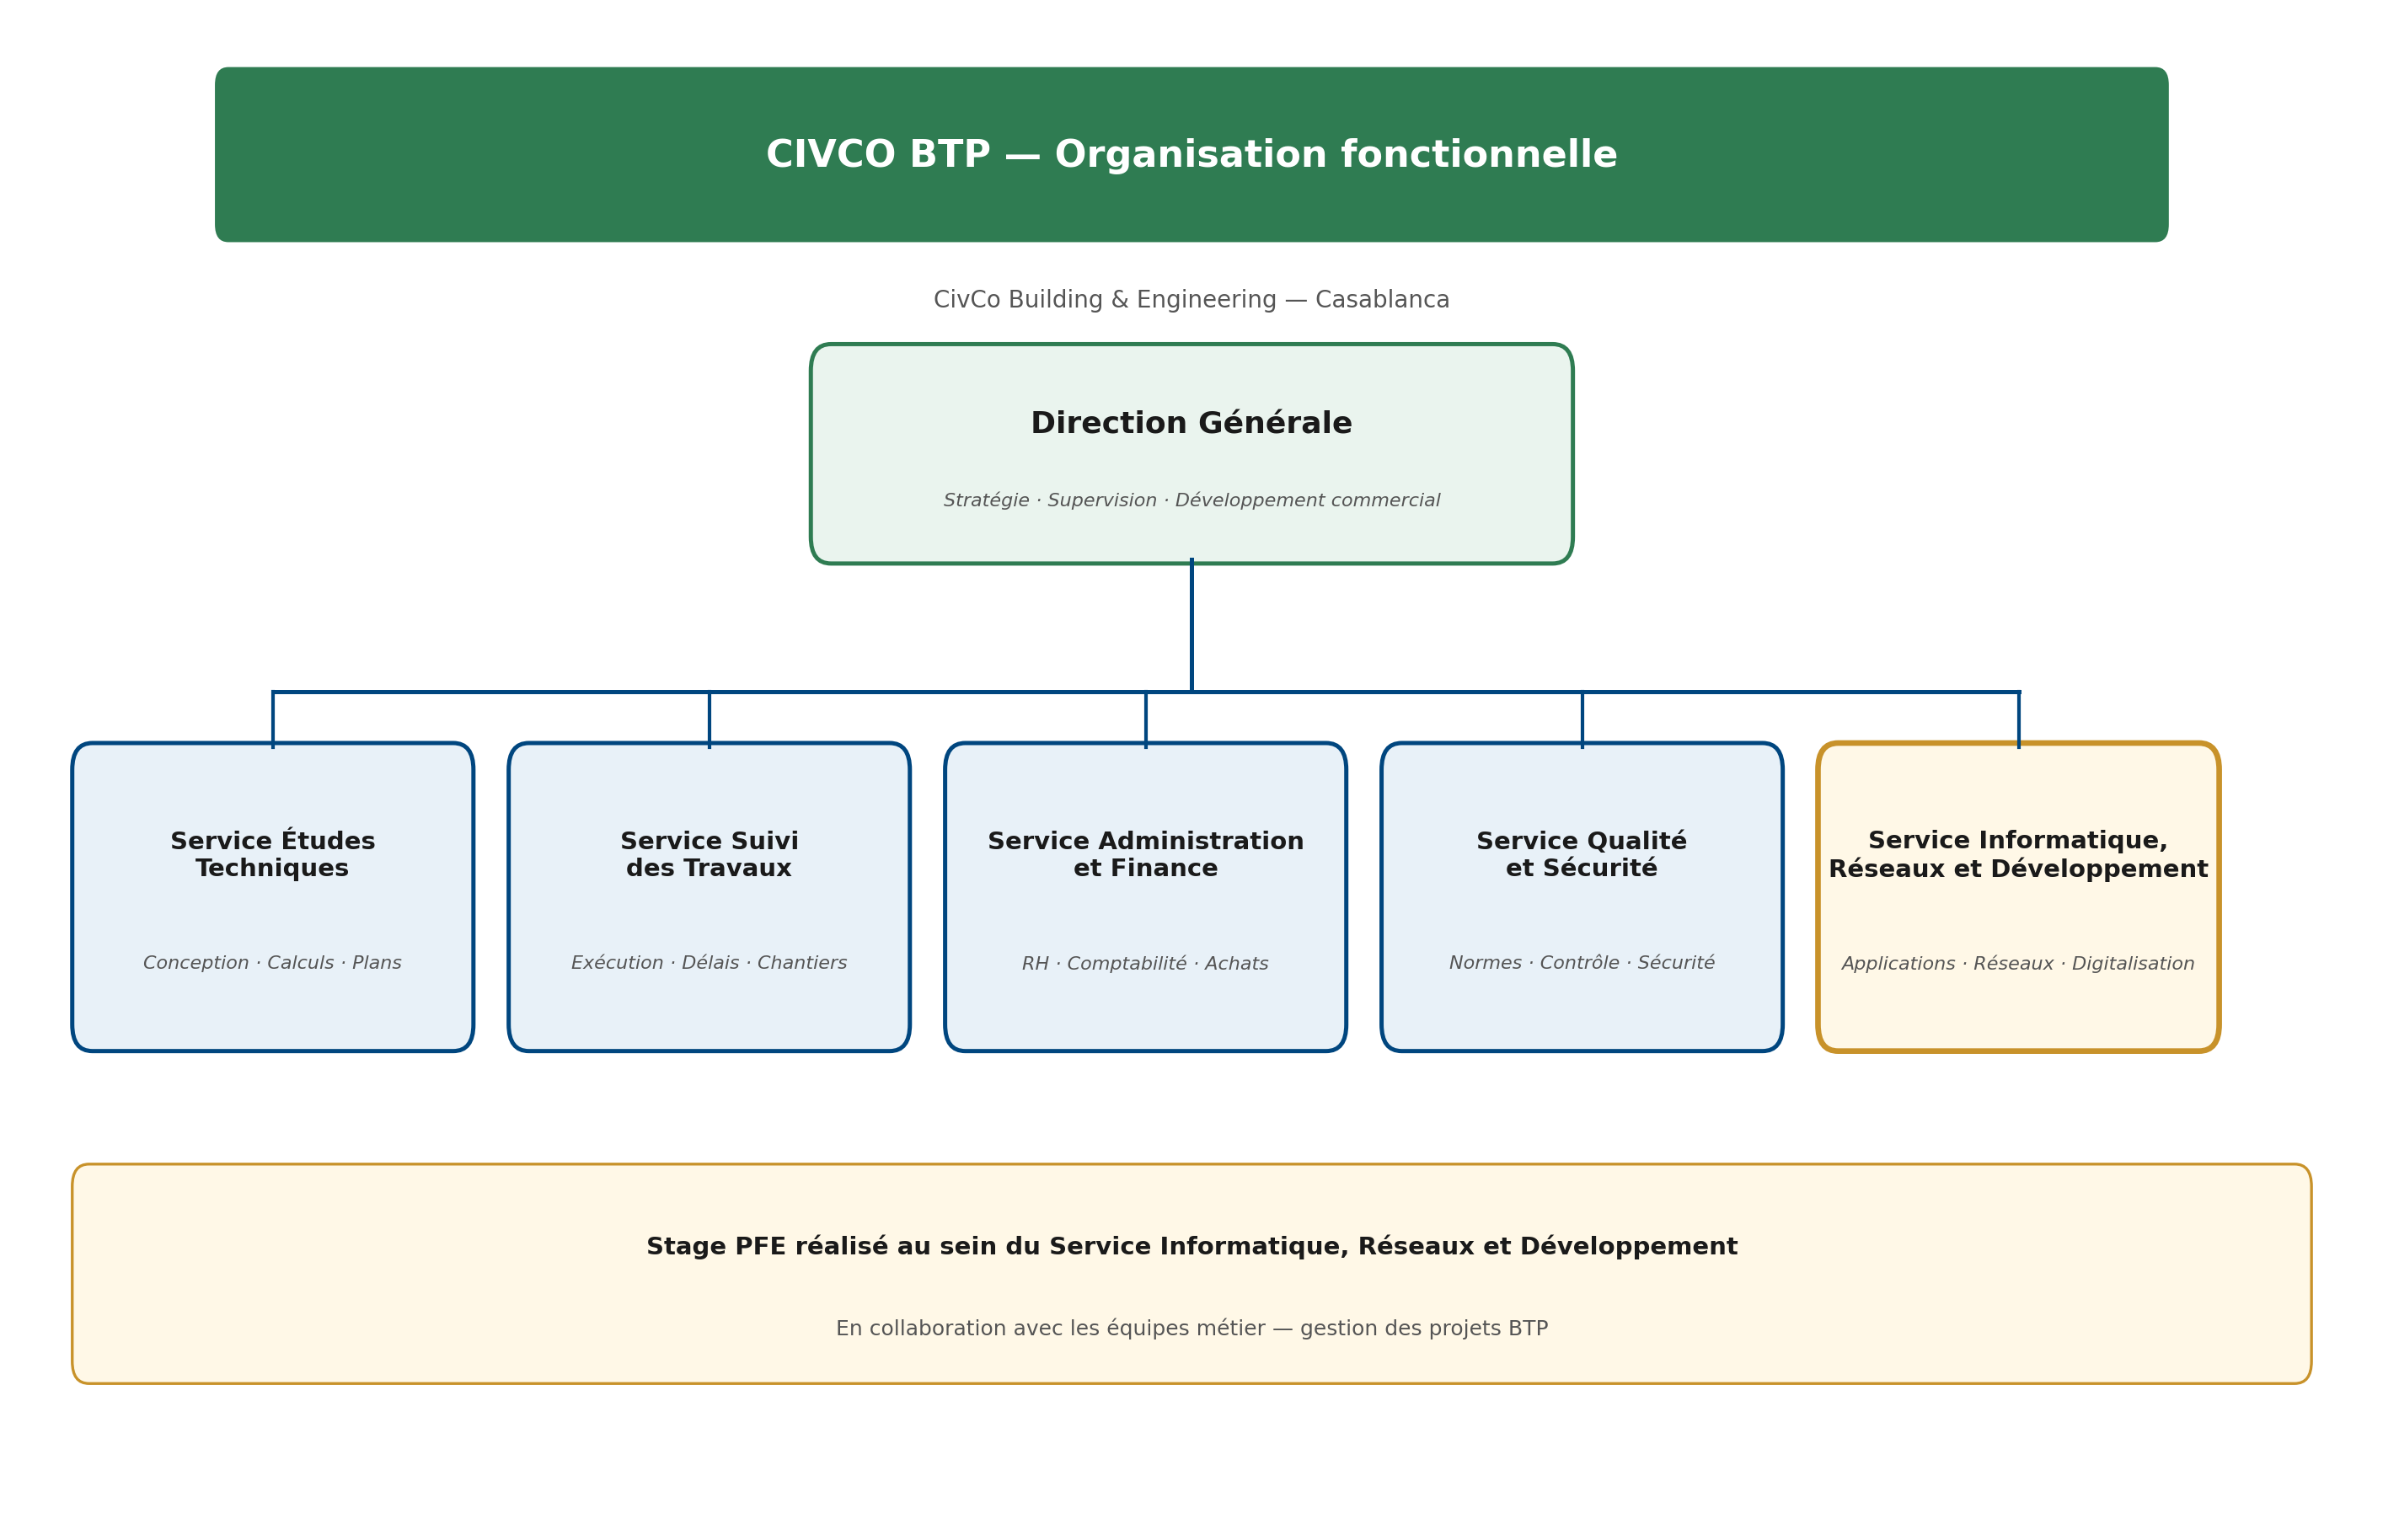
\includegraphics[width=0.85\textwidth]{departments.png}
  \caption{Organisation fonctionnelle de CIVCO BTP}
  \label{fig:civco_org}
\end{figure}

Ce stage s'est déroulé au sein du \textbf{Service Informatique, Réseaux et Développement},
en étroite collaboration avec les équipes métier concernées par la gestion des projets.

\subsection{Domaines d'activité}

Les activités de CIVCO BTP couvrent plusieurs domaines complémentaires :

\medskip

\textbf{Génie civil et études de structures.} Études de bâtiments résidentiels et
industriels, ouvrages publics et infrastructures ; calcul en béton armé, structures
métalliques, dimensionnement des fondations et vérification de stabilité.

\medskip

\textbf{Assistance technique et conseil.} Assistance à maîtrise d'ouvrage, contrôle des
travaux, coordination des intervenants, réception des ouvrages, expertise technique,
études de faisabilité et optimisation des solutions constructives.

\medskip

\textbf{Informatique et développement.} Développement d'applications web et de logiciels
métiers, conception et administration de bases de données, maintenance applicative,
sécurisation des systèmes d'information et déploiement de solutions numériques au service
de la productivité et du suivi des projets.

\medskip

\textbf{Exemples de projets réalisés.} CIVCO BTP intervient sur des chantiers de natures
variées, illustrant la diversité de son portefeuille :

\begin{itemize}
  \item \textbf{Bâtiments résidentiels} : immeubles collectifs, villas haut standing,
  lotissements avec voirie et réseaux.
  \item \textbf{Ouvrages industriels} : halls de production, entrepôts logistiques,
  extensions d'usines existantes.
  \item \textbf{Infrastructures publiques} : voiries urbaines, ouvrages d'assainissement,
  aménagements d'espaces publics.
  \item \textbf{Rénovation et réhabilitation} : mise aux normes parasismiques, extension
  de bâtiments patrimoniaux, restructuration de locaux tertiaires.
\end{itemize}

Cette diversité impose à l'entreprise une capacité d'adaptation et un suivi rigoureux
de chaque affaire, renforçant le besoin d'un outil de gestion centralisé.

\subsection{Moyens humains et matériels}

\textbf{Moyens humains.} L'entreprise s'appuie sur une équipe pluridisciplinaire :
direction générale, ingénieurs génie civil et structures, dessinateurs-projeteurs,
conducteurs de travaux, techniciens, développeurs informatiques, administrateurs réseaux
et systèmes, personnel administratif et financier. Cette diversité de compétences permet
de répondre aux exigences techniques et organisationnelles des projets confiés à CIVCO BTP.

\medskip

\textbf{Moyens matériels.} Sur le plan technique, l'entreprise dispose d'un parc
informatique (postes de travail, serveurs, équipements réseau), de logiciels de conception
(AutoCAD, Revit, Robot Structural Analysis), d'outils de développement (Visual Studio Code,
Git, GitHub) et de systèmes de gestion de bases de données (MySQL, PostgreSQL, SQL Server).
Des véhicules de chantier, une connectivité haut débit et des plateformes collaboratives
complètent l'environnement de travail.

\section{Analyse de l'existant}

Avant de définir la solution cible, une phase d'observation et d'entretiens a été
menée auprès des différents services de CIVCO BTP. L'objectif était de comprendre
comment l'information circule aujourd'hui, quels sont les points de friction et
quels gains une application intégrée pourrait apporter.

\subsection{Processus métier actuels}

Le cycle de vie d'un projet de construction chez CIVCO BTP peut se décomposer en
plusieurs étapes successives, impliquant des acteurs distincts :

\begin{enumerate}
  \item \textbf{Prospection et relation client} : identification du besoin, échanges
  préliminaires, constitution de la fiche client (coordonnées, contacts, historique).
  \item \textbf{Étude et chiffrage} : analyse technique, estimation des coûts,
  production d'un devis détaillé avec lignes de prestations.
  \item \textbf{Contractualisation} : rédaction du contrat, éventuels avenants en cas
  de modification du périmètre ou du budget.
  \item \textbf{Planification} : découpage en phases, affectation de l'équipe,
  définition des tâches opérationnelles et des jalons.
  \item \textbf{Exécution} : suivi de chantier, mise à jour de l'avancement,
  production des bons de livraison et des documents de suivi.
  \item \textbf{Facturation et clôture} : émission des factures, suivi des paiements,
  archivage du dossier projet.
\end{enumerate}

Chaque étape génère des documents et des données qui doivent être partagés entre
le service commercial, les ingénieurs, les conducteurs de travaux, la comptabilité
et parfois le client final. Aujourd'hui, cette circulation repose en grande partie
sur des échanges manuels.

\subsection{Cartographie des outils utilisés}

Le Tableau~\ref{tab:outils_existants} synthétise les outils actuellement mobilisés
par service et leurs limites respectives.

\begin{table}[H]
\caption{Outils actuels et limites identifiées}
\label{tab:outils_existants}
\centering
\small
\begin{tabular}{|l|p{4.2cm}|p{5.8cm}|}
\hline
\textbf{Service} & \textbf{Outils} & \textbf{Limites observées} \\
\hline
Commercial & Excel, Word, courriel & Devis non centralisés, ressaisies \\
\hline
Études / Projets & AutoCAD, Revit, fichiers partagés & Pas de lien avec le suivi financier \\
\hline
Chantier & WhatsApp, tableurs & Informations éphémères, peu traçables \\
\hline
Comptabilité & Logiciel comptable, PDF & Saisie manuelle des factures \\
\hline
Direction & Rapports ponctuels & Absence de tableau de bord temps réel \\
\hline
\end{tabular}
\end{table}

Cette cartographie a confirmé l'absence d'un \textbf{référentiel unique} reliant
clients, projets, documents et équipes. Chaque service dispose de sa propre
organisation documentaire, ce qui complique la consolidation des indicateurs et
la reprise d'information lors d'un changement d'interlocuteur.

\subsection{Besoins exprimés par les services}

Les entretiens menés avec l'encadrant professionnel et les responsables de service
ont permis de formaliser les attentes prioritaires :

\begin{itemize}
  \item \textbf{Direction} : vision consolidée de l'activité (projets actifs,
  retards, charge des équipes).
  \item \textbf{Commercial} : création rapide de devis, historique client,
  conversion simplifiée en facture.
  \item \textbf{Ingénieurs / chefs de projet} : suivi des phases, des tâches et
  de l'équipe affectée à chaque chantier.
  \item \textbf{Comptabilité} : accès aux factures, suivi des paiements et état
  de facturation par projet.
  \item \textbf{Clients} : consultation de l'avancement et validation des
  documents sans dépendre des échanges par courriel.
\end{itemize}

Ces besoins ont orienté le périmètre fonctionnel de l'application développée.

\section{Contexte et problématique}

\subsection{Constats et limites des pratiques actuelles}

Au quotidien, la gestion des projets de construction chez CIVCO BTP mobilise plusieurs
services : études techniques, suivi de travaux, administration, finance et qualité.
Chaque chantier génère un volume important d'informations --- clients, phases, tâches,
devis, factures, contrats, bons de livraison --- qui doivent être partagées entre les
intervenants.

Or, une partie de ces processus repose encore sur des outils non intégrés : fichiers
Excel, documents Word ou PDF isolés, échanges par courriel ou messagerie instantanée.
Cette dispersion entraîne plusieurs difficultés :

\begin{itemize}
  \item \textbf{Fragmentation de l'information} : les données d'un même projet sont
  éparpillées entre plusieurs fichiers et supports.
  \item \textbf{Manque de visibilité} : difficulté à disposer d'une vue d'ensemble sur
  l'avancement des chantiers et des tâches en cours.
  \item \textbf{Risque d'erreurs} : ressaisies manuelles, versions multiples de documents
  et absence de source unique de vérité.
  \item \textbf{Lenteur de coordination} : dépendance aux échanges informels entre
  services pour obtenir une information à jour.
\end{itemize}

\subsection{Problématique}

Face à l'augmentation du nombre de projets et à la complexité croissante de leur suivi,
CIVCO BTP a identifié le besoin de disposer d'un \textbf{outil numérique centralisé} dédié
à la gestion et à la planification de ses projets de construction.

\medskip

La problématique de ce projet peut se formuler ainsi :

\begin{quote}
\textit{Comment concevoir et développer une application web permettant à CIVCO BTP de
centraliser, structurer et piloter l'ensemble du cycle de vie de ses projets de
construction, tout en s'adaptant aux différents profils métier de l'entreprise ?}
\end{quote}

\section{Périmètre du projet}

\subsection{Fonctionnalités incluses}

Le périmètre retenu pour ce stage couvre les modules suivants, considérés comme
prioritaires pour une première version exploitable en interne :

\begin{itemize}
  \item Authentification sécurisée et gestion des rôles (\textbf{RBAC}).
  \item Gestion des projets (phases, équipe, avancement, géolocalisation).
  \item Gestion des clients et provisionnement du portail externe.
  \item Production des documents commerciaux (devis, factures, bons de livraison).
  \item Suivi contractuel (contrats, avenants, modèles de documents).
  \item Planification et suivi des tâches opérationnelles.
  \item Tableau de bord, carte des chantiers et historique des actions.
  \item Messagerie projet entre équipe interne et client.
\end{itemize}

\subsection{Limites et hors périmètre}

Certains sujets ont été volontairement exclus ou reportés à une phase ultérieure,
afin de concentrer l'effort de développement sur le cœur métier :

\begin{itemize}
  \item \textbf{Comptabilité générale} : l'application gère les factures et
  paiements projet, mais ne remplace pas le logiciel comptable de l'entreprise.
  \item \textbf{CAO / BIM} : les outils de conception (AutoCAD, Revit) restent
  indépendants ; seules les métadonnées projet sont centralisées.
  \item \textbf{Gestion des stocks} : non couverte dans cette version.
  \item \textbf{Application mobile native} : l'interface responsive web est
  privilégiée ; une application dédiée est envisagée en perspective.
  \item \textbf{Interopérabilité ERP tiers} : pas d'intégration avec des solutions
  externes (SAP, Sage, etc.) dans le cadre de ce stage.
\end{itemize}

Cette délimitation garantit un livrable cohérent et testable dans la durée du stage,
tout en laissant une base évolutive pour les extensions futures.

\section{Objectifs du projet}

\subsection{Objectif général}

Concevoir et développer une \textbf{application web} de gestion et de planification des
projets de construction pour CIVCO BTP, capable de couvrir les principaux processus métier
liés au suivi des chantiers et à la production des documents commerciaux.

\subsection{Objectifs fonctionnels}

\begin{itemize}
  \item \textbf{Gestion des projets} : créer, consulter et suivre les chantiers par phases,
  avec affectation des équipes et suivi de l'avancement.
  \item \textbf{Gestion des clients} : centraliser les informations clients, contacts et
  historique des projets associés.
  \item \textbf{Documents commerciaux} : produire et suivre les devis, factures et bons de
  livraison (\textbf{BL}) liés aux projets.
  \item \textbf{Suivi contractuel} : gérer les contrats et les avenants associés aux
  chantiers.
  \item \textbf{Planification des tâches} : organiser le travail opérationnel par phases
  et attribuer les tâches aux collaborateurs.
  \item \textbf{Tableau de bord} : offrir une vue synthétique de l'activité (projets en
  cours, indicateurs clés, tâches prioritaires).
  \item \textbf{Contrôle d'accès} : garantir que chaque utilisateur accède uniquement aux
  fonctionnalités correspondant à son rôle (\textbf{RBAC}).
\end{itemize}

\subsection{Objectifs techniques}

\begin{itemize}
  \item Mettre en place une architecture \textit{full-stack} avec un \textit{backend} API
  \textbf{Laravel} / \textbf{PHP} et une interface \textbf{React} en \textbf{SPA}.
  \item Concevoir une base de données relationnelle (\textbf{SQL}) modélisant les entités
  métier (projets, clients, documents, utilisateurs, rôles).
  \item Exposer des services \textbf{REST} sécurisés pour la communication entre le
  \textit{frontend} et le \textit{backend}.
  \item Assurer une interface ergonomique, responsive et adaptée à un usage professionnel
  quotidien.
  \item Valider le bon fonctionnement des modules développés par des tests manuels et,
  le cas échéant, des tests automatisés.
\end{itemize}

\section{Méthodologie adoptée}

\subsection{Démarche de développement}

Le projet a été mené selon une approche \textbf{itérative et incrémentale}, adaptée au
contexte d'un stage en entreprise. Le travail s'est déroulé en plusieurs étapes :

\begin{enumerate}
  \item \textbf{Analyse des besoins} : recueil des attentes auprès de l'encadrant
  professionnel et identification des modules prioritaires.
  \item \textbf{Conception} : modélisation des entités métier, définition de l'architecture
  technique et des cas d'utilisation principaux.
  \item \textbf{Développement par modules} : implémentation progressive des fonctionnalités
  (projets, clients, documents commerciaux, tâches, tableau de bord, etc.).
  \item \textbf{Tests et validation} : vérification du comportement de chaque module et
  correction des anomalies identifiées.
  \item \textbf{Documentation} : rédaction du présent rapport et documentation technique
  du code produit.
\end{enumerate}

Chaque itération visait à livrer un incrément fonctionnel, démontrable lors des réunions
de suivi, avant de passer au module suivant.

\subsection{Gestion de projet avec Trello}

Le suivi opérationnel du stage a été organisé à l'aide de \textbf{Trello}, outil de
gestion de projet en ligne basé sur la méthode \textbf{Kanban}. Un tableau dédié au
projet regroupait les tâches sous forme de cartes réparties en colonnes selon leur
état : \textit{À faire}, \textit{En cours}, \textit{En revue} et \textit{Terminé}.

\medskip

Chaque carte correspondait à une fonctionnalité, une correction ou une tâche de
conception (par exemple : « Module devis --- API backend », « Écran tableau de bord »,
« Tests RoleAccess »). Les cartes précisaient une brève description, une priorité et,
le cas échéant, une échéance. Cette organisation a permis de :

\begin{itemize}
  \item visualiser l'avancement global du projet en un coup d'œil ;
  \item prioriser les modules à développer en accord avec l'encadrant professionnel ;
  \item conserver une trace des tâches réalisées et de celles restant à traiter ;
  \item préparer les démonstrations lors des réunions de suivi hebdomadaires.
\end{itemize}

Trello a ainsi complété Git/GitHub : le premier pour la planification et le suivi
des livrables métier, le second pour le versionnement du code source.

\subsection{Suivi académique et professionnel}

\textbf{Suivi académique (EMSI Casablanca) :}
\begin{itemize}
  \item Encadrant pédagogique : \textbf{Pr. Mohammed El Assad}
  \item Réunions régulières de suivi, validation de la démarche et préparation de la
  soutenance finale.
\end{itemize}

\textbf{Suivi professionnel (CIVCO BTP) :}
\begin{itemize}
  \item Encadrant professionnel : \textbf{M. Mohamed BENABDELLAH-CHAOUNI}
  \item Réunions de suivi pour présenter l'avancement, valider les choix fonctionnels et
  recueillir les retours métier.
  \item Alignement continu du développement avec les besoins réels de l'entreprise.
\end{itemize}

\subsection{Outils et environnement de travail}

\textbf{Outils de développement :}
\begin{itemize}
  \item \textbf{Trello} : gestion de projet et suivi des tâches (tableau Kanban).
  \item \textbf{Git / GitHub} : gestion de versions et suivi des évolutions du code.
  \item \textbf{Visual Studio Code} : environnement de développement principal.
  \item \textbf{Laravel} : framework \textit{backend} (\textbf{MVC}, \textbf{ORM} Eloquent).
  \item \textbf{React + Vite} : interface utilisateur (\textbf{SPA}).
  \item \textbf{MySQL / PostgreSQL} : base de données relationnelle.
\end{itemize}

\textbf{Environnements :}
\begin{itemize}
  \item \textbf{Développement} : poste local avec serveur Laravel et serveur de
  développement Vite (\textit{hot-reload}).
  \item \textbf{Tests} : validation manuelle des parcours utilisateurs et tests
  fonctionnels sur les modules livrés.
\end{itemize}

\section{Planification du stage}

Le stage s'est déroulé sur la période \textbf{avril -- juillet 2026}, au sein du service
informatique de CIVCO BTP. La planification générale du projet peut se résumer comme suit :

\begin{table}[H]
\centering
\caption{Phases principales du projet de stage}
\label{tab:planification}
\begin{tabularx}{\textwidth}{|l|X|}
\hline
\textbf{Phase} & \textbf{Activités principales} \\
\hline
Analyse & Étude de l'existant, recueil des besoins, définition du périmètre \\
\hline
Conception & Modélisation UML, architecture technique, maquettage des interfaces \\
\hline
Développement & Implémentation progressive des modules (\textit{backend} et \textit{frontend}) \\
\hline
Tests & Vérification fonctionnelle, corrections et stabilisation \\
\hline
Rédaction & Rédaction du rapport de fin d'études et préparation de la soutenance \\
\hline
\end{tabularx}
\end{table}

\subsection{Planning détaillé par période}

Le Tableau~\ref{tab:planning_detail} détaille la répartition des activités sur
les quatre mois du stage. Chaque période correspond à un jalon de démonstration
validé avec l'encadrant professionnel.

\begin{table}[H]
\centering
\caption{Planning détaillé du stage (avril -- juillet 2026)}
\label{tab:planning_detail}
\small
\begin{tabularx}{\textwidth}{|l|X|}
\hline
\textbf{Période} & \textbf{Livrables et activités} \\
\hline
Avril 2026 &
Analyse de l'existant, entretiens métier, rédaction du cahier des charges fonctionnel,
validation du périmètre avec l'encadrant professionnel \\
\hline
Mai 2026 &
Conception UML (cas d'utilisation, séquence, classes), modélisation de la base de données,
architecture technique three-tier, maquettage des écrans principaux \\
\hline
Juin 2026 &
Développement backend Laravel (authentification, projets, clients, devis, factures),
mise en place du frontend React (navigation, tableau de bord), premières démonstrations
des modules livrés \\
\hline
Juillet 2026 &
Portail client, tâches, configuration des rôles, tests PHPUnit et validation manuelle,
stabilisation, rédaction du rapport de fin d'études et préparation de la soutenance \\
\hline
\end{tabularx}
\end{table}

\medskip

Cette planification incrémentale a permis de livrer des modules testables au fur
et à mesure, tout en ajustant les priorités en fonction des retours terrain.
Par exemple, le module d'impression documentaire et le suivi des copies officielles
ont été intégrés en cours de développement suite à une demande exprimée par la
direction administrative.

\newpage
\section*{Conclusion}

Ce chapitre a posé le cadre du projet de fin d'études réalisé au sein de
\textbf{CIVCO BTP}. Nous avons présenté l'organisme d'accueil, son organisation
et les domaines d'activité du bureau d'études, afin de situer le projet dans son
contexte métier BTP. L'analyse de l'existant a mis en évidence la dispersion des
outils (tableurs, documents isolés, échanges informels) et la difficulté à disposer
d'une vision consolidée des chantiers, des clients et des documents commerciaux.

\medskip

À partir de cette problématique, nous avons formulé les objectifs fonctionnels et
techniques de l'application : centraliser la gestion des projets, des clients, des
devis, des factures et du suivi opérationnel, tout en garantissant un contrôle
d'accès par rôles adapté aux différents profils de l'entreprise. Le périmètre retenu
couvre les modules prioritaires identifiés avec l'encadrant professionnel, dans une
logique de livrable progressif et testable.

\medskip

La méthodologie adoptée combine une approche \textbf{agile incrémentale}, un suivi
\textbf{Kanban} via \textbf{Trello} et un versionnement \textbf{Git/GitHub}.
Le planning sur quatre mois (avril -- juillet 2026) a structuré les phases d'analyse,
de conception, de développement et de validation, avec des jalons de démonstration
réguliers. Ce cadrage constitue la base sur laquelle s'appuient les chapitres
suivants.

\medskip

Le chapitre suivant expose l'état de l'art des technologies mobilisées et justifie
les choix techniques retenus --- architecture \textit{full-stack}, \textbf{Laravel},
\textbf{React} et base de données relationnelle --- pour la réalisation de
l'application.

% \chapter{État de l'Art et Étude Théorique}
\label{chap:etat_art}

\section{Introduction}

L'application développée pour CIVCO BTP s'appuie sur un ensemble de technologies web
modernes, réparties entre un \textit{backend} API, une base de données relationnelle et
une interface utilisateur riche. Ce chapitre constitue le socle théorique du rapport :
il présente les concepts et les technologies étudiés, puis justifie les choix retenus
pour la réalisation du projet.

\medskip

Nous abordons successivement les \textbf{architectures des applications web}, le
\textbf{framework Laravel} côté serveur, les \textbf{interfaces React en SPA}, les
\textbf{bases de données relationnelles et l'ORM}, les \textbf{API REST et
l'authentification}, ainsi que les \textbf{solutions ERP et outils de gestion de projets
dans le secteur du BTP}. Le chapitre se conclut par une référence comparative
(\textit{benchmark}) justifiant chaque choix technologique retenu.

% ─────────────────────────────────────────────────────────────────────
\section{Les applications web et l'architecture full-stack}
\subsection{Évolution des applications web}

Les applications de gestion d'entreprise ont connu une évolution majeure au cours des
deux dernières décennies. Les premières solutions reposaient sur des architectures
\textbf{monolithiques} : logique métier, interface et base de données regroupées dans
un même programme, souvent accessible via un navigateur avec rechargement complet de
page à chaque action.

\medskip

L'émergence des \textbf{API} (\textit{Application Programming Interface}) a séparé la
couche de présentation de la couche métier. Le navigateur ou une application mobile
consomme des services distants via \textbf{HTTP}, échangeant des données structurées en
\textbf{JSON}. Cette découpe a ouvert la voie aux architectures \textit{full-stack}
modernes, dans lesquelles un \textit{frontend} JavaScript riche dialogue avec un
\textit{backend} API indépendant~\cite{fielding2000rest}.

\subsection{Architecture client-serveur et tiers}

L'architecture \textbf{three-tier} (\textit{trois tiers}) structure l'application en
trois couches distinctes :

\begin{enumerate}
  \item \textbf{Couche présentation} : interface utilisateur (React), exécutée dans le
  navigateur.
  \item \textbf{Couche métier} : logique applicative, règles de gestion, authentification
  (Laravel).
  \item \textbf{Couche données} : persistance relationnelle (MySQL / PostgreSQL).
\end{enumerate}

Cette séparation améliore la maintenabilité : chaque couche peut évoluer indépendamment
tant que les contrats d'interface (API REST) sont respectés. Fowler~\cite{fowler2019patterns}
décrit ce découpage comme un patron fondamental des applications d'entreprise.

\begin{figure}[H]
  \centering
  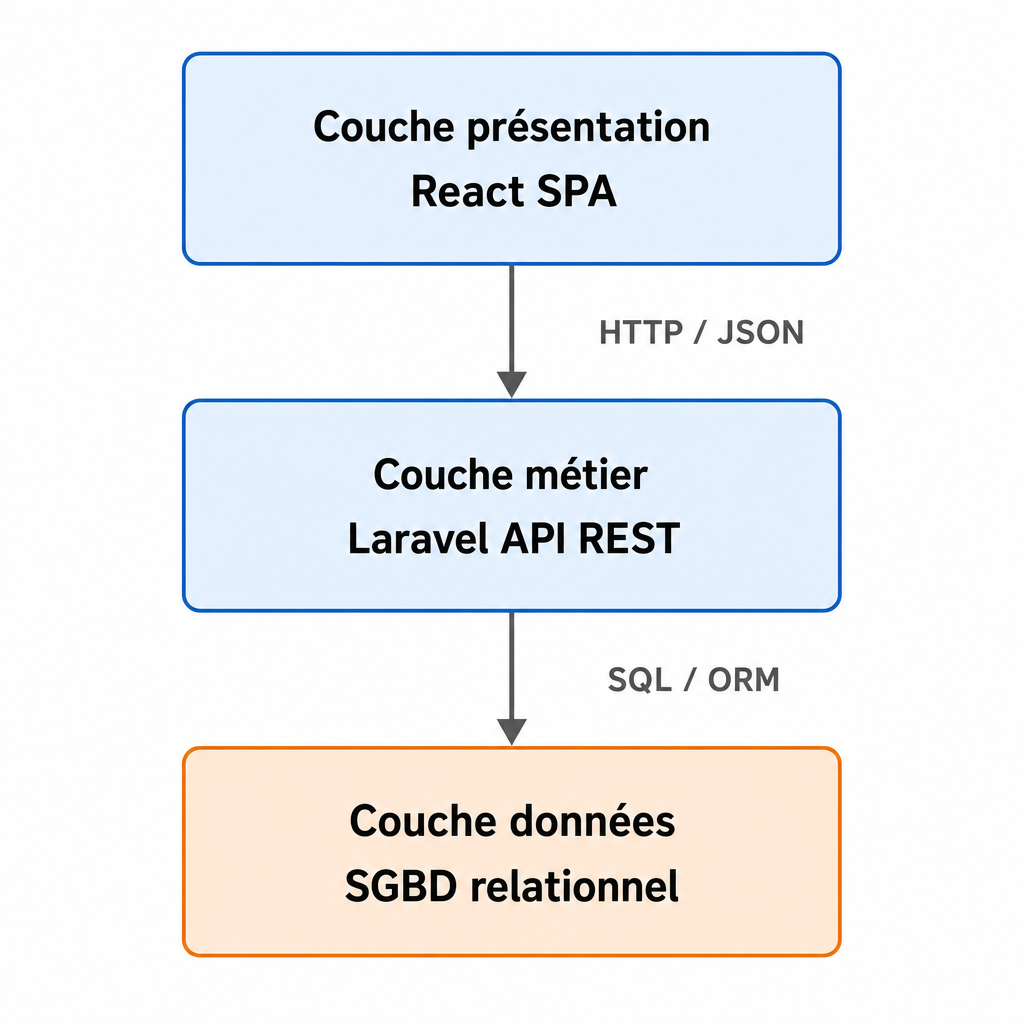
\includegraphics[width=0.55\textwidth]{fig_2_1_three_tier_preview.png}
  \caption{Architecture three-tier de l'application CIVCO BTP}
  \label{fig:three_tier}
\end{figure}

\subsection{Single Page Application (SPA)}

Une \textbf{SPA} (\textit{Single Page Application}) charge une seule page HTML, puis
met à jour dynamiquement le contenu via JavaScript sans rechargement complet. Les
avantages pour une application métier sont significatifs :

\begin{itemize}
  \item \textbf{Fluidité} : navigation instantanée entre les modules (projets, clients,
  factures).
  \item \textbf{Expérience utilisateur} : interfaces réactives, proches des applications
  de bureau.
  \item \textbf{Réutilisation de l'état} : conservation du contexte utilisateur
  (filtres, session) entre les écrans.
\end{itemize}

Le couplage d'une SPA React avec une API Laravel constitue aujourd'hui un standard
industriel pour les tableaux de bord et outils de gestion internes.

\subsection{Panorama des stacks full-stack}

\begin{table}[H]
\caption{Panorama des stacks full-stack pour applications métier}
\label{tab:stack_panorama}
\centering
\small
\begin{tabular}{|l|l|p{8cm}|}
\hline
\textbf{Stack} & \textbf{Langages} & \textbf{Caractéristiques} \\
\hline
LAMP / LEMP & PHP + MySQL & Mature, hébergement abordable, Laravel/Symfony \\
\hline
MERN / MEAN & JavaScript & Un seul langage, Node.js + MongoDB \\
\hline
Django + React & Python + JS & Rapidité backend, ORM Django \\
\hline
\textbf{Laravel + React} & PHP + JS & API REST + SPA, écosystème riche \\
\hline
.NET + Angular & C\# + TS & Écosystème Microsoft, entreprise \\
\hline
\end{tabular}
\end{table}

Pour CIVCO BTP, la stack \textbf{Laravel + React} (Tableau~\ref{tab:stack_panorama})
offre le meilleur compromis entre productivité, courbe d'apprentissage et adéquation
avec les compétences visées en filière IIR : développement web, bases de données et
architecture logicielle.

\subsection{Échange de données et format JSON}

Les API modernes échangent des données structurées en \textbf{JSON} (\textit{JavaScript
Object Notation}), format léger et lisible, natif en JavaScript et bien supporté par
PHP/Laravel. Chaque ressource métier est sérialisée en objet JSON : un projet expose
son identifiant, son client associé, ses phases, son statut et ses dates ; un devis
expose ses lignes, montants et statut de validation.

\medskip

Ce format facilite le découplage frontend/backend : React consomme directement les
réponses JSON, les mappe vers ses composants et met à jour l'interface sans
transformation complexe. Les codes de statut HTTP (\texttt{200}, \texttt{201},
\texttt{422}, \texttt{403}) signalent le résultat de chaque opération de façon
standardisée.

\subsection{Patterns CRUD et ressources métier}

La majorité des modules de l'application suivent le pattern \textbf{CRUD}
(\textit{Create, Read, Update, Delete}) : créer un client, lister les projets,
modifier une facture, archiver un document. Laravel formalise ce pattern via les
contrôleurs de ressources et les routes RESTful, ce qui garantit une cohérence
d'API sur l'ensemble des modules (clients, projets, devis, factures, tâches,
contrats).


% ─────────────────────────────────────────────────────────────────────
\section{Le framework Laravel et l'écosystème PHP}
\subsection{Présentation de PHP et Laravel}

\textbf{PHP} est un langage de script côté serveur largement déployé sur le web.
Historiquement associé au développement de sites dynamiques, il a évolué vers des
versions modernes (8.x) intégrant un typage strict, des performances accrues (JIT) et
un écosystème mature de frameworks.

\medskip

\textbf{Laravel}~\cite{laravel} est le framework PHP le plus adopté pour construire des
applications web et des API. Créé par Taylor Otwell, il impose une structure claire
autour du patron \textbf{MVC} (\textit{Model-View-Controller}) et propose des
composants intégrés pour les tâches courantes : routage, validation, authentification,
files d'attente, envoi de courriels et gestion des fichiers.

\subsection{Architecture MVC dans Laravel}

Le patron \textbf{MVC} répartit les responsabilités :

\begin{itemize}
  \item \textbf{Modèle} : représentation des entités métier et accès aux données
  (Eloquent).
  \item \textbf{Vue} : dans une API, les \textit{Resources} et \textit{Collections}
  formatent les réponses JSON pour le client.
  \item \textbf{Contrôleur} : reçoit la requête HTTP, applique la validation, invoque
  les services métier et retourne la réponse.
\end{itemize}

Cette organisation facilite la lecture du code et l'ajout de nouveaux modules. Pour
l'application CIVCO BTP, chaque domaine métier (projets, clients, devis, factures)
dispose de son contrôleur, de ses modèles et de ses règles de validation.

\subsection{Composants clés de l'écosystème Laravel}

\subsubsection{Routage et validation}

Le fichier de routes (\texttt{routes/api.php}) déclare les points d'entrée de l'API.
Chaque route est associée à un contrôleur et protégée par des \textit{middleware}
(vérification d'authentification, contrôle de permissions, contexte entreprise).

Les \textbf{Form Requests} encapsulent les règles de validation des données entrantes
(ex.~: champs obligatoires d'un devis, formats de dates, montants positifs), garantissant
l'intégrité des données avant persistance.

\subsubsection{Services et logique métier}

Au-delà des contrôleurs, la logique complexe est extraite dans des classes
\textbf{Service} (\texttt{QuoteService}, \texttt{PrintTrackingService}, etc.). Ce
découpage respecte le principe de responsabilité unique : le contrôleur orchestre,
le service implémente la règle métier.

\subsubsection{Migrations et seeders}

Les \textbf{migrations} versionnent le schéma de la base de données sous forme de fichiers
PHP exécutables de façon reproductible. Les \textbf{seeders} initialisent des données
de référence (rôles, permissions, données de démonstration), indispensables pour
tester l'application en conditions proches du réel.

\subsection{Comparaison avec les alternatives PHP}

\begin{table}[H]
\caption{Comparaison des frameworks PHP pour une API REST}
\label{tab:php_frameworks}
\centering
\small
\begin{tabular}{|l|p{4cm}|p{4cm}|p{4cm}|}
\hline
\textbf{Framework} & \textbf{Philosophie} & \textbf{Forces} & \textbf{Contexte idéal} \\
\hline
\textbf{Laravel} & Convention over configuration & Écosystème complet, Sanctum, Eloquent &
API + SPA, PME/ETI \\
\hline
Symfony & Composants réutilisables & Modularité, robustesse & Grandes applications \\
\hline
CodeIgniter & Minimaliste & Légèreté & Petits projets \\
\hline
\end{tabular}
\end{table}

Laravel ressort du Tableau~\ref{tab:php_frameworks} pour un projet de gestion métier
nécessitant authentification, RBAC, documents et évolutivité --- le profil exact du
projet CIVCO BTP.

\subsection{Laravel dans le projet CIVCO BTP}

L'API Laravel expose plus de quarante contrôleurs organisés par domaine, des
\textit{middleware} de contrôle d'accès et un ensemble de services métier. Cette
structure permet d'ajouter progressivement de nouveaux modules (avenants contractuels,
modèles de documents, suivi d'impression) sans remettre en cause l'architecture
existante.

\subsection{Middleware, Resources et couche de présentation API}

\subsubsection{Middleware}

Les \textbf{middleware} Laravel interceptent chaque requête HTTP avant qu'elle
n'atteigne le contrôleur. Dans le projet, plusieurs middlewares assurent la
sécurité et le contexte métier :

\begin{itemize}
  \item \textbf{Authentification Sanctum} : vérifie que l'utilisateur est connecté.
  \item \textbf{Contrôle de permissions} : valide que l'utilisateur possède la
  permission requise (\texttt{project.view}, \texttt{quote.manage}, etc.).
  \item \textbf{Contexte entreprise} : identifie la société courante via l'en-tête
  \texttt{X-Company-Id}, garantissant l'isolation des données métier.
\end{itemize}

\subsubsection{API Resources}

Les classes \textbf{Resource} (\texttt{ProjectResource}, \texttt{InvoiceResource},
etc.) transforment les modèles Eloquent en tableaux JSON normalisés. Elles permettent
de contrôler précisément les champs exposés à l'interface, d'inclure conditionnellement
des relations (\texttt{client}, \texttt{lines}, \texttt{teamMembers}) et d'uniformiser
le format de réponse sur toute l'API.

\subsubsection{Validation et gestion des erreurs}

Lorsqu'une requête échoue la validation, Laravel retourne une réponse \texttt{422}
avec le détail des champs en erreur. Le frontend React intercepte ces réponses pour
afficher des messages à l'utilisateur, améliorant l'expérience de saisie sur les
formulaires de devis, factures et fiches projets.


% ─────────────────────────────────────────────────────────────────────
\section{React et les Single Page Applications}
\subsection{Définition et principes des SPA}

Une \textbf{SPA} (\textit{Single Page Application}) est une application web dont
l'interface est construite dynamiquement en JavaScript. Contrairement aux sites
classiques où chaque clic déclenche un rechargement HTML complet, la SPA charge le
shell de l'application une fois, puis met à jour le DOM (\textit{Document Object Model})
au fil des interactions utilisateur.

\medskip

Ce modèle repose sur le \textbf{routing côté client} : la bibliothèque React Router
associe chaque URL à un composant React (\texttt{/projects}, \texttt{/clients},
\texttt{/invoices}), sans solliciter le serveur pour le HTML. Seules les données
nécessaires sont récupérées via l'API REST.

\subsection{React : bibliothèque declarative}

\textbf{React}~\cite{react}, développé par Meta, est une bibliothèque JavaScript pour
construire des interfaces utilisateur par \textbf{composants} réutilisables. Chaque
composant encapsule structure (JSX), état et comportement.

\medskip

Les principes fondamentaux de React sont :

\begin{itemize}
  \item \textbf{Composants fonctionnels} : fonctions JavaScript retournant du JSX,
  composées hiérarchiquement (Sidebar, Dashboard, ProjectDetailPage, etc.).
  \item \textbf{État local} (\texttt{useState}) : données modifiables au sein d'un
  composant (formulaires, filtres, modales).
  \item \textbf{Effets de bord} (\texttt{useEffect}) : chargement de données API au
  montage du composant ou lors d'un changement de paramètre.
  \item \textbf{Context API} : partage d'état global (authentification, thème, langue)
  sans propager les props à travers toute l'arborescence.
\end{itemize}

Cette approche declarative simplifie la construction d'interfaces complexes : l'état
de l'interface est une fonction de l'état applicatif.

\subsection{Écosystème React du projet}

L'application CIVCO BTP s'appuie sur plusieurs bibliothèques complémentaires :

\begin{table}[H]
\caption{Composants de l'écosystème frontend}
\label{tab:react_ecosystem}
\centering
\small
\begin{tabular}{|l|l|p{7.5cm}|}
\hline
\textbf{Outil} & \textbf{Rôle} & \textbf{Usage dans le projet} \\
\hline
Vite~\cite{vite} & Build tool & Compilation rapide, HMR en développement \\
\hline
React Router & Routing & Navigation entre modules ERP \\
\hline
Axios & Client HTTP & Appels API REST avec intercepteurs \\
\hline
Tailwind CSS~\cite{tailwindcss} & Styles utilitaires & Interface sombre cohérente \\
\hline
Recharts & Graphiques & Tableau de bord, KPIs \\
\hline
Leaflet & Cartographie & Carte des projets / chantiers \\
\hline
\end{tabular}
\end{table}

\subsection{Communication avec le backend}

Le \textit{frontend} React consomme l'API Laravel via des modules dédiés
(\texttt{api/projects.js}, \texttt{api/clients.js}, etc.). Un client Axios centralisé
configure :

\begin{itemize}
  \item l'envoi automatique des cookies de session (Sanctum) ;
  \item le jeton CSRF pour les requêtes \texttt{POST}, \texttt{PUT} et \texttt{DELETE} ;
  \item la gestion des erreurs \texttt{401} (redirection vers la page de connexion).
\end{itemize}

Ce patron \textit{API-first} garantit que toute action utilisateur (créer un devis,
archiver un client, assigner une tâche) transite par la couche métier Laravel, où les
règles de validation et de permissions sont appliquées.

\begin{figure}[H]
\centering
\resizebox{0.92\textwidth}{!}{%
\begin{tikzpicture}[
  box/.style={rectangle, rounded corners=4pt, fill=ensamBlue!12, draw=ensamBlue,
              minimum width=3.2cm, minimum height=1.0cm, align=center,
              font=\small\bfseries},
  arr/.style={-{Stealth[length=6pt]}, thick, draw=gray!70},
  lbl/.style={font=\footnotesize, text=gray!70}
]
  \node[box] (browser) at (0, 0)   {Navigateur\\React SPA};
  \node[box] (api)     at (5.5, 0) {API Laravel\\REST + Sanctum};
  \node[box] (db)      at (11, 0)  {Base de\\données};

  \draw[arr] (browser) -- (api) node[midway, above, lbl] {JSON / HTTPS};
  \draw[arr] (api)     -- (db)  node[midway, above, lbl] {Eloquent / SQL};
\end{tikzpicture}
}%
\caption{Flux de communication React $\rightarrow$ Laravel $\rightarrow$ SGBD}
\label{fig:react_flow}
\end{figure}

\subsection{Comparaison React / Vue / Angular}

\begin{table}[H]
\caption{Comparaison des principaux frameworks frontend (2025-2026)}
\label{tab:spa_compare}
\centering
\small
\begin{tabular}{|l|p{3.5cm}|p{3.5cm}|p{3.5cm}|}
\hline
\textbf{Critère} & \textbf{React} & \textbf{Vue.js} & \textbf{Angular} \\
\hline
Flexibilité & Élevée (bibliothèque) & Élevée (progressif) & Opinionated (framework complet) \\
\hline
Courbe d'apprentissage & Modérée & Faible & Élevée \\
\hline
Marché de l'emploi & Très large & Large & Large (entreprise) \\
\hline
Écosystème SPA & React Router, Vite & Vue Router, Vite & Router intégré \\
\hline
\end{tabular}
\end{table}

React est retenu pour sa flexibilité, son adoption industrielle et la disponibilité de
bibliothèques adaptées aux tableaux de bord métier (graphiques, cartes, composants
modulaires), comme le montre le Tableau~\ref{tab:spa_compare}.

\subsection{Organisation du code frontend}

Le code React est structuré par \textbf{features} (\texttt{features/projects/},
\texttt{features/clients/}, \texttt{features/invoices/}), chacune regroupant pages,
composants et utilitaires propres au module. Les composants transverses (Sidebar,
PermissionGate, modales) vivent dans \texttt{components/}. Cette organisation par
domaine facilite la navigation dans le code et l'ajout de nouvelles fonctionnalités
sans impacter les modules existants.

\subsection{Interface utilisateur et Tailwind CSS}

L'interface adopte un design sombre professionnel, cohérent sur tous les modules.
\textbf{Tailwind CSS}~\cite{tailwindcss} est un framework CSS utilitaire : les classes
(\texttt{flex}, \texttt{rounded-lg}, \texttt{bg-gray-800}) s'appliquent directement
dans le JSX. Cette approche accélère le prototypage et garantit une cohérence visuelle
sur les écrans de l'application (listes, fiches détail, modales, tableaux de bord).

\medskip

Le \textbf{tableau de bord} illustre l'intérêt de React pour la visualisation métier :
graphiques (Recharts), widgets configurables, indicateurs \textbf{KPI} et accès rapide
aux projets en cours. La carte des chantiers (Leaflet) offre une vue géographique des
projets, pertinente pour une entreprise disposant de plusieurs sites simultanés.

\subsection{Internationalisation}

L'application supporte le \textbf{français} (langue par défaut) et l'\textbf{anglais}
via un contexte de langue et des fichiers de traduction (\texttt{locales/fr.js},
\texttt{locales/en.js}). Cette préparation facilite l'usage de l'outil par des
collaborateurs anglophones ou une future extension à d'autres contextes linguistiques.


% ─────────────────────────────────────────────────────────────────────
\section{Les bases de données relationnelles et l'ORM}

\subsection{Modèle relationnel et SGBD}

Une application de gestion de projets manipule des entités fortement structurées et
liées entre elles : clients, projets, phases, tâches, devis, factures, contrats,
utilisateurs et rôles. Le \textbf{modèle relationnel}, formalisé par Codd, organise ces
données en tables reliées par des clés étrangères, garantissant l'intégrité référentielle
et la cohérence des enregistrements~\cite{fowler2019patterns}.

\medskip

Les \textbf{SGBD} (\textit{Systèmes de Gestion de Bases de Données}) relationnels les
plus répandus en environnement web sont \textbf{MySQL}~\cite{mysql} et
\textbf{PostgreSQL}~\cite{postgresql}. MySQL se distingue par sa simplicité de déploiement
et sa large adoption ; PostgreSQL offre des fonctionnalités avancées (contraintes
complexes, types JSON, performances sur de gros volumes). Pour une application métier
comme celle de CIVCO BTP, les deux systèmes conviennent ; le choix final dépend de
l'environnement d'hébergement et des besoins de montée en charge.

\subsection{L'ORM et Eloquent}

Manipuler directement le langage \textbf{SQL} dans chaque composant applicatif alourdit
le code et complique la maintenance. L'\textbf{ORM} (\textit{Object-Relational Mapping})
fait correspondre les tables de la base à des classes du langage de programmation.
Dans Laravel, \textbf{Eloquent} fournit une couche d'abstraction élégante :

\begin{itemize}
  \item chaque table est représentée par un \textbf{modèle} (\texttt{Project},
  \texttt{Client}, \texttt{Invoice}, etc.) ;
  \item les relations (\texttt{hasMany}, \texttt{belongsTo}, \texttt{belongsToMany})
  expriment les liens métier de façon déclarative ;
  \item les migrations versionnent le schéma de la base et facilitent le déploiement
  entre environnements ;
  \item les \textit{seeders} permettent de peupler la base avec des données de démonstration.
\end{itemize}

Cette approche accélère le développement, réduit les erreurs de requêtes et aligne le
code objet sur le modèle métier de l'entreprise.

\subsection{Normalisation et intégrité des données}

La conception d'une base pour un ERP léger repose sur plusieurs principes :

\begin{itemize}
  \item \textbf{Normalisation} : éviter la duplication d'informations (un client est
  enregistré une seule fois, référencé par ses projets et documents).
  \item \textbf{Contraintes d'intégrité} : clés étrangères, unicité des identifiants
  métier (numéros de devis, de facture).
  \item \textbf{Traçabilité} : horodatage des enregistrements (\texttt{created\_at},
  \texttt{updated\_at}) et journalisation des actions sensibles.
\end{itemize}

Ces principes sont essentiels dans un contexte BTP où les documents commerciaux et
contractuels doivent rester cohérents et auditables.

\subsection{Modèle de données métier}

Le schéma relationnel de l'application modélise les entités principales du cycle de
vie d'un projet CIVCO BTP :

\begin{table}[H]
\centering
\small
\caption{Entités principales du modèle de données}
\label{tab:entities}
\begin{tabular}{|l|p{9cm}|}
\hline
\textbf{Entité} & \textbf{Rôle} \\
\hline
Client & Maître d'ouvrage ou client commercial, contacts associés \\
\hline
Project & Chantier / projet, lié à un client, phases et équipe \\
\hline
ProjectPhase & Découpage temporel du projet (études, exécution, réception) \\
\hline
Task & Tâche opérationnelle assignée à un collaborateur \\
\hline
Quote / Invoice & Documents commerciaux avec lignes de détail \\
\hline
Contract & Contrat et avenants liés au projet \\
\hline
User / Role & Utilisateurs internes et permissions RBAC \\
\hline
\end{tabular}
\end{table}

Les relations entre ces entités (un client possède plusieurs projets, un projet
contient plusieurs phases et tâches, un devis peut être converti en facture) sont
implémentées via Eloquent et contraintes de clés étrangères en base.

% ─────────────────────────────────────────────────────────────────────
\section{Les API REST et l'authentification}

\subsection{Principe des API REST}

Une \textbf{API REST} (\textit{Representational State Transfer}) expose des ressources
(identifiées par des URL) manipulables via les verbes \textbf{HTTP} :
\texttt{GET} (lecture), \texttt{POST} (création), \texttt{PUT/PATCH} (mise à jour),
\texttt{DELETE} (suppression)~\cite{fielding2000rest}. Ce style architectural sépare
clairement le \textit{frontend} (interface utilisateur) du \textit{backend} (logique
métier et persistance), ce qui permet :

\begin{itemize}
  \item de faire évoluer l'interface sans réécrire le serveur ;
  \item de réutiliser la même API pour d'éventuels clients mobiles futurs ;
  \item de tester indépendamment chaque couche.
\end{itemize}

Dans le projet CIVCO BTP, l'API est organisée sous le préfixe \texttt{/api/v1/} et
expose des ressources métier : projets, clients, devis, factures, tâches, etc.

\subsection{Authentification et contrôle d'accès}

La sécurisation d'une application métier repose sur deux piliers :

\medskip

\textbf{Authentification.} Laravel \textbf{Sanctum}~\cite{sanctum} gère l'authentification
par session pour les applications \textbf{SPA} : le navigateur conserve un cookie de
session sécurisé, complété par une protection \textbf{CSRF} (\textit{Cross-Site Request
Forgery}) sur les requêtes mutantes. Cette approche est adaptée à une application hébergée
sur le même domaine que l'API, sans la complexité d'un flux JWT (\textit{JSON Web Token})
côté client.

\medskip

\textbf{Autorisation (RBAC).} Le contrôle d'accès basé sur les rôles (\textbf{RBAC})
associe à chaque utilisateur un ensemble de permissions (\texttt{project.view},
\texttt{quote.manage}, \texttt{invoice.view}, etc.). Les routes API vérifient ces
permissions avant d'exécuter l'action demandée. Ainsi, un commercial, un chef de
projet et un administrateur accèdent chacun aux modules correspondant à leur profil
métier.

% ─────────────────────────────────────────────────────────────────────
\section{ERP et digitalisation du secteur BTP}

\subsection{Enjeux de la gestion intégrée en BTP}

Le secteur du \textbf{BTP} partage avec l'industrie des besoins de traçabilité, de
planification et de coordination documentaire. Un \textbf{ERP} (\textit{Enterprise
Resource Planning}) vise à unifier ces processus : relation client, suivi de chantier,
achats, facturation, ressources humaines. Dans le BTP, les spécificités suivantes
renforcent l'intérêt d'un outil intégré :

\begin{itemize}
  \item multiplicité des intervenants (MOA, BET, entreprises, sous-traitants) ;
  \item cycle documentaire riche (devis, bons de commande, BL, factures, avenants) ;
  \item suivi temporel des phases et des tâches de chantier ;
  \item besoin de visibilité consolidée pour la direction et les conducteurs de travaux.
\end{itemize}

\subsection{Panorama des solutions existantes}

Le marché propose des solutions generalistes et des outils spécialisés construction :

\begin{table}[H]
\centering
\small
\caption{Panorama de solutions de gestion applicables au BTP}
\label{tab:erp_panorama}
\begin{tabular}{|l|l|p{7.5cm}|}
\hline
\textbf{Solution} & \textbf{Type} & \textbf{Apport principal} \\
\hline
SAP S/4HANA & ERP generaliste & Suite intégrée grande entreprise, modules finance et projets \\
\hline
Sage 100 / X3 & ERP PME & Comptabilité, commercial, gestion de production \\
\hline
Procore~\cite{procore} & SaaS BTP & Gestion de projets construction, documents, coordination \\
\hline
Buildertrend & SaaS BTP & Suivi chantier, relation client, devis \\
\hline
Solution sur mesure & Développement interne & Adaptation exacte aux processus de l'entreprise \\
\hline
\end{tabular}
\end{table}

Les ERP generalistes offrent une couverture fonctionnelle large mais imposent des coûts
de licence, de paramétrage et de formation élevés. Les solutions SaaS BTP sont plus
ciblées mais restent standardisées. Pour CIVCO BTP, le développement d'une
\textbf{application sur mesure} permet d'aligner précisément l'outil sur les processus
internes, tout en maîtrisant l'évolution fonctionnelle.

\subsection{Digitalisation des BET au Maroc}

Les bureaux d'études techniques marocains, comme CIVCO BTP, combinent expertise
ingénierie et activités de suivi de chantier. La digitalisation de leurs processus
internes --- gestion documentaire, suivi des échéances, coordination inter-services ---
constitue un levier de compétitivité. Une application web interne permet de :

\begin{itemize}
  \item réduire le temps de recherche d'information sur un projet ;
  \item standardiser la production des devis et factures ;
  \item améliorer la visibilité de l'avancement pour la direction et les conducteurs ;
  \item préparer une traçabilité des actions (journal d'activité, historique).
\end{itemize}

Ce contexte sectoriel justifie l'investissement dans une solution adaptée plutôt que
dans un ERP generaliste surdimensionné pour la taille et les processus de l'entreprise.

% ─────────────────────────────────────────────────────────────────────
\section{Références comparatives (Benchmarks) et justification des choix}

\subsection{Comparaison des frameworks backend}

\begin{table}[H]
\centering
\small
\caption{Comparaison des frameworks backend pour une API métier}
\label{tab:backend_benchmark}
\begin{tabular}{|l|p{3.2cm}|p{3.2cm}|p{3cm}|}
\hline
\textbf{Framework} & \textbf{Points forts} & \textbf{Limites} & \textbf{Écosystème} \\
\hline
\textbf{Laravel} & ORM Eloquent, migrations, Sanctum, rapidité de dev & Performance brute inférieure à Go/Rust & Très riche (PHP) \\
\hline
Symfony & Modularité, robustesse entreprise & Courbe d'apprentissage plus longue & Large (PHP) \\
\hline
Django & Admin intégré, ORM puissant & Moins adapté aux SPA modernes & Python \\
\hline
Express.js & Légèreté, JavaScript full-stack & Structure laissée au développeur & Node.js \\
\hline
\end{tabular}
\end{table}

\textbf{Laravel}~\cite{laravel} ressort du Tableau~\ref{tab:backend_benchmark} pour sa
productivité, son ORM mature, son système d'authentification Sanctum adapté aux SPA et
sa documentation exhaustive --- critères décisifs pour un projet de stage avec délai
contraint.

\subsection{Comparaison des frameworks frontend}

\begin{table}[H]
\centering
\small
\caption{Comparaison des frameworks frontend}
\label{tab:frontend_benchmark}
\begin{tabular}{|l|c|c|c|c|}
\hline
\textbf{Framework} & \textbf{Popularité} & \textbf{Écosystème} & \textbf{Courbe} &
\textbf{SPA} \\
\hline
\textbf{React} & Très élevée & Très riche & Modérée & Native \\
\hline
Vue.js & Élevée & Riche & Faible & Native \\
\hline
Angular & Élevée & Complet (Google) & Élevée & Native \\
\hline
Svelte & Croissante & Moyen & Faible & Native \\
\hline
\end{tabular}
\end{table}

\textbf{React}~\cite{react} est retenu (Tableau~\ref{tab:frontend_benchmark}) pour son
écosystème (React Router, bibliothèques UI), sa adoption industrielle massive et sa
compatibilité avec \textbf{Vite}~\cite{vite} pour un cycle de développement rapide.

\subsection{Comparaison des SGBD}

\begin{table}[H]
\centering
\small
\caption{Comparaison des systèmes de gestion de bases de données}
\label{tab:db_benchmark}
\begin{tabular}{|l|c|c|c|c|}
\hline
\textbf{SGBD} & \textbf{Open source} & \textbf{JSON} & \textbf{Performance} &
\textbf{Déploiement} \\
\hline
\textbf{MySQL} & Oui & Partiel & Élevée & Simple \\
\hline
\textbf{PostgreSQL} & Oui & Natif & Très élevée & Standard \\
\hline
SQLite & Oui & Oui & Faible (fichier) & Très simple \\
\hline
SQL Server & Non & Oui & Élevée & Entreprise \\
\hline
\end{tabular}
\end{table}

MySQL et PostgreSQL conviennent toutes deux au projet ; PostgreSQL est privilégié en
production pour sa robustesse, MySQL ou SQLite pouvant servir en développement local.

\subsection{Synthèse des choix}

\begin{table}[H]
\caption{Synthèse des choix technologiques et critères décisifs}
\label{tab:tech_choices}
\centering
\small
\begin{tabular}{|l|l|p{7cm}|}
\hline
\textbf{Composant} & \textbf{Choix retenu} & \textbf{Critère décisif} \\
\hline
Backend & Laravel 13 / PHP 8.3 & Productivité, ORM, écosystème mature \\
\hline
Frontend & React 19 + Vite 8 & SPA réactive, écosystème riche \\
\hline
Style UI & Tailwind CSS 4~\cite{tailwindcss} & Développement rapide, cohérence visuelle \\
\hline
API & REST / JSON & Simplicité, séparation frontend/backend \\
\hline
Authentification & Laravel Sanctum & Sessions SPA sécurisées, CSRF \\
\hline
Base de données & MySQL / PostgreSQL & Modèle relationnel, intégrité \\
\hline
ORM & Eloquent & Mapping objet-relationnel, migrations \\
\hline
Contrôle d'accès & RBAC (rôles/permissions) & Profils métier CIVCO BTP \\
\hline
\end{tabular}
\end{table}

Le Tableau~\ref{tab:tech_choices} récapitule l'ensemble des choix retenus pour
l'application de gestion de projets de CIVCO BTP.

% ─────────────────────────────────────────────────────────────────────
\section{Méthodologies de développement logiciel}

\subsection{Approches traditionnelles et agiles}

Le développement d'une application métier peut suivre différentes méthodologies.
L'approche \textbf{cascade} (\textit{Waterfall}) enchaîne les phases de manière
séquentielle : analyse, conception, développement, tests, déploiement. Elle convient
aux projets dont les besoins sont stables et parfaitement définis en amont, mais
peut s'avérer rigide lorsque les exigences évoluent en cours de réalisation.

\medskip

Les méthodes \textbf{agiles}~\cite{agilemanifesto}, à l'inverse, privilégient des
itérations courtes (sprints de deux à quatre semaines), une collaboration continue
avec le client et l'adaptation au changement. Le \textbf{Manifeste Agile} (2001)
formalise quatre valeurs : individus et interactions plutôt que processus et outils,
logiciel fonctionnel plutôt que documentation exhaustive, collaboration client plutôt
que négociation contractuelle, adaptation au changement plutôt que suivi d'un plan
rigide.

\subsection{Application au projet CIVCO BTP}

Dans le contexte de ce stage, une approche \textbf{itérative et incrémentale} a été
retenue, s'inspirant des principes agiles. Le suivi des tâches a été matérialisé via
\textbf{Trello}, organisé selon un tableau \textbf{Kanban} (colonnes \textit{À faire},
\textit{En cours}, \textit{Terminé}), sans appliquer un cadre Scrum formel (sprints,
daily meetings). Les raisons de ce choix sont les suivantes :

\begin{itemize}
  \item \textbf{Périmètre évolutif} : les besoins métier ont été affinés au fil des
  démonstrations, notamment pour les modules d'impression et de portail client.
  \item \textbf{Durée limitée} : quatre mois de stage imposent des livrables réguliers
  plutôt qu'une phase d'analyse prolongée.
  \item \textbf{Proximité métier} : l'encadrant professionnel était disponible pour
  valider chaque incrément et orienter les priorités.
  \item \textbf{Risque maîtrisé} : chaque module livré est testable indépendamment,
  réduisant le risque d'une intégration finale décevante.
\end{itemize}

\subsection{Qualité logicielle et bonnes pratiques}

Indépendamment de la méthodologie, plusieurs principes de qualité logicielle ont
guidé le développement :

\begin{itemize}
  \item \textbf{Principe DRY} (\textit{Don't Repeat Yourself}) : factorisation de
  la logique commune dans des services et des composants réutilisables.
  \item \textbf{Principe SOLID} : responsabilité unique des classes (un service par
  domaine métier), injection de dépendances via le conteneur Laravel.
  \item \textbf{Conventions de code} : Laravel Pint pour le PHP, ESLint pour le
  JavaScript, respect des standards PSR-12 et des conventions React.
  \item \textbf{Tests automatisés} : couverture des flux critiques (authentification,
  CRUD, conversion devis) par PHPUnit pour détecter les régressions.
  \item \textbf{Documentation} : commentaires sur les règles métier complexes,
  présent rapport et annexes techniques.
\end{itemize}

Ces pratiques, combinées à l'architecture modulaire décrite aux chapitres suivants,
visent à produire un code maintenable et évolutif, au-delà de la seule durée du stage.

\newpage
\section*{Conclusion}

Ce chapitre a posé les fondements théoriques et technologiques sur lesquels repose
l'application développée pour CIVCO BTP. Nous avons d'abord rappelé l'évolution des
applications web vers des architectures \textit{full-stack} en trois tiers, dans
lesquelles la couche présentation (React), la couche métier (Laravel) et la couche
données (SGBD relationnel) sont clairement séparées. Ce découplage facilite la
maintenance, les tests et l'évolution indépendante de chaque composant.

\medskip

L'étude de \textbf{Laravel} a montré comment un framework PHP mature structure le
\textit{backend} autour du patron \textbf{MVC}, d'Eloquent, de migrations et de
Sanctum. Les middleware, les Form Requests et les API Resources garantissent à la
fois la sécurité, la validation des données et un format de réponse JSON cohérent
pour l'ensemble des modules métier.

\medskip

Côté interface, \textbf{React} permet de construire une \textbf{SPA} modulaire et
réactive, organisée par fonctionnalités et appuyée sur un écosystème riche (Vite,
Axios, Tailwind CSS, Recharts, Leaflet). L'échange permanent entre le navigateur et
l'API REST via JSON constitue le lien central de l'architecture retenue.

\medskip

Le modèle relationnel et l'\textbf{ORM} assurent l'intégrité et la cohérence des
données --- clients, projets, phases, tâches, devis, factures et contrats --- tandis
que le \textbf{RBAC} adapte l'accès aux différents profils métier de l'entreprise.
Enfin, le panorama des solutions ERP et BTP a situé le projet dans son contexte
sectoriel et confirmé la pertinence d'une application sur mesure pour CIVCO BTP.

\medskip

Les benchmarks comparatifs ont permis de justifier chaque choix : Laravel pour la
productivité backend, React pour l'expérience utilisateur, PostgreSQL/MySQL pour la
persistance, Sanctum pour l'authentification SPA. L'ensemble de ces décisions est
guidé par trois impératifs : la \textbf{productivité} de développement dans le cadre
du stage, la \textbf{maintenabilité} du code sur le long terme, et l'\textbf{adéquation
métier} aux processus internes de l'entreprise.

\medskip

Le chapitre suivant traduit ces choix en une architecture système concrète : analyse
des besoins, identification des acteurs, cas d'utilisation et modélisation
\textbf{UML} de l'application de gestion et de planification des projets de
construction.

\newpage

% \chapter{Conception du Système}
\label{chap:conception}

\section{Introduction}

Ce chapitre présente la phase de conception de l'application développée pour CIVCO BTP.
Il traduit les besoins métier identifiés au Chapitre~1 en spécifications techniques
formelles et en modèles architecturaux. Nous commençons par identifier les acteurs et
leurs cas d'utilisation, puis nous définissons les exigences fonctionnelles et
non-fonctionnelles du système. Nous décrivons ensuite l'architecture retenue, la
conception des modules métier principaux, et nous terminons par la modélisation
\textbf{UML} : diagrammes de cas d'utilisation, de séquence, de classes et d'activité.

% ─────────────────────────────────────────────────────────────────────
\section{Analyse des besoins}

\subsection{Identification des acteurs}

Six catégories d'acteurs interagissent avec l'application de gestion de CIVCO BTP :

\begin{description}
  \item[Administrateur] Responsable de la configuration globale de l'application :
  gestion des utilisateurs, des rôles et permissions, des paramètres documentaires,
  du thème visuel et de la consultation de l'historique des actions.
  \item[Chef de projet] Pilote un ou plusieurs chantiers : suivi des phases et des
  tâches, affectation des équipes, consultation des documents liés au projet,
  gestion des contrats et des avenants.
  \item[Commercial] Gère la relation client et les documents commerciaux : création
  et suivi des devis, conversion en factures, production des bons de livraison.
  \item[Comptable] Assure le suivi financier : consultation et validation des
  factures, suivi des paiements, état de facturation par projet.
  \item[Utilisateur interne] Collaborateur terrain ou technique assigné à des tâches
  spécifiques : consultation de ses missions, mise à jour de l'avancement, accès
  limité aux projets auxquels il est affecté.
  \item[Client externe] Maître d'ouvrage ou client final accédant au portail dédié
  pour consulter l'état de ses projets, accepter les devis, signer les contrats et
  échanger avec l'équipe CIVCO BTP.
\end{description}

\subsection{Cas d'utilisation}

Les cas d'utilisation principaux, regroupés par domaine fonctionnel, sont les suivants :

\textbf{Authentification et tableau de bord :}
\begin{itemize}
  \item UC-01 : S'authentifier à l'application (connexion sécurisée par session).
  \item UC-02 : Consulter le tableau de bord synthétique (projets en cours, tâches,
  indicateurs clés).
\end{itemize}

\textbf{Gestion des projets :}
\begin{itemize}
  \item UC-03 : Créer et modifier un projet de construction (référence, client, budget,
  dates, localisation).
  \item UC-04 : Définir les phases d'un projet et suivre l'avancement global.
  \item UC-05 : Affecter des membres d'équipe à un projet.
  \item UC-06 : Consulter la carte géographique des chantiers.
\end{itemize}

\textbf{Gestion des clients :}
\begin{itemize}
  \item UC-07 : Créer, modifier et archiver une fiche client.
  \item UC-08 : Gérer les contacts associés à un client.
  \item UC-09 : Provisionner un accès portail pour un client externe.
\end{itemize}

\textbf{Documents commerciaux :}
\begin{itemize}
  \item UC-10 : Créer un devis avec lignes de détail et le lier à un projet.
  \item UC-11 : Convertir un devis accepté en facture.
  \item UC-12 : Émettre un bon de livraison (\textbf{BL}) lié à un projet.
  \item UC-13 : Imprimer ou exporter un document commercial (devis, facture, BL).
\end{itemize}

\textbf{Contrats et tâches :}
\begin{itemize}
  \item UC-14 : Créer et suivre un contrat associé à un projet.
  \item UC-15 : Enregistrer un avenant contractuel (modification budget/durée).
  \item UC-16 : Créer, assigner et suivre des tâches opérationnelles.
\end{itemize}

\textbf{Administration et portail client :}
\begin{itemize}
  \item UC-17 : Configurer les rôles, permissions et paramètres de l'application.
  \item UC-18 : Consulter le journal d'activité et l'historique des actions.
  \item UC-19 : Échanger des messages avec un client via la messagerie intégrée.
  \item UC-20 : (Client externe) Consulter ses projets, accepter un devis, signer
  un contrat via le portail.
\end{itemize}

\subsection{Exigences fonctionnelles}

\begin{itemize}
  \item \textbf{EF-01 Authentification :} Connexion par email et mot de passe via
  Laravel Sanctum (session sécurisée par cookie, protection \textbf{CSRF}).
  \item \textbf{EF-02 Gestion des rôles :} Attribution de rôles métier (administrateur,
  chef de projet, commercial, comptable, utilisateur) avec permissions granulaires
  (\textbf{RBAC}).
  \item \textbf{EF-03 Gestion des projets :} \textbf{CRUD} complet sur les projets,
  avec phases, équipe, budget, avancement, géolocalisation du chantier.
  \item \textbf{EF-04 Gestion des clients :} Fiches clients, contacts, archivage,
  provisionnement d'accès portail.
  \item \textbf{EF-05 Devis :} Création de devis multi-lignes, calcul automatique des
  totaux HT/TVA/TTC, suivi des statuts (brouillon, envoyé, accepté, refusé).
  \item \textbf{EF-06 Factures :} Conversion devis $\rightarrow$ facture, suivi de
  l'état de paiement, numérotation automatique.
  \item \textbf{EF-07 Bons de livraison :} Production de BL liés aux projets, avec
  lignes de détail et suivi des quantités livrées.
  \item \textbf{EF-08 Contrats :} Gestion des contrats et avenants, compilation à
  partir de modèles, double signature (entreprise + client).
  \item \textbf{EF-09 Tâches :} Planification par phase, assignation, statuts
  (à faire, en cours, terminé), filtrage par utilisateur.
  \item \textbf{EF-10 Tableau de bord :} Widgets configurables (projets actifs,
  tâches prioritaires, graphiques d'avancement).
  \item \textbf{EF-11 Portail client :} Interface dédiée pour consultation des projets,
  acceptation de devis et signature de contrats.
  \item \textbf{EF-12 Messagerie :} Échanges projet-scopés entre équipe interne et
  client externe.
  \item \textbf{EF-13 Historique :} Journalisation des actions sensibles (création,
  modification, archivage) consultable par l'administrateur.
\end{itemize}

\subsection{Exigences non-fonctionnelles}

\textbf{Performance :}
\begin{itemize}
  \item \textbf{ENF-01 :} Temps de réponse des API inférieur à 500~ms pour les
  opérations de lecture courantes (listes, fiches détail).
  \item \textbf{ENF-02 :} Chargement initial de l'interface (SPA) inférieur à 3~s
  sur une connexion standard.
\end{itemize}

\textbf{Sécurité :}
\begin{itemize}
  \item \textbf{ENF-03 :} Mots de passe hachés (bcrypt) ; sessions Sanctum avec
  expiration configurable.
  \item \textbf{ENF-04 :} Contrôle d'accès par permission sur chaque route API ;
  vérification côté serveur avant toute action métier.
  \item \textbf{ENF-05 :} Protection \textbf{CSRF} sur les requêtes mutantes ;
  communication \textbf{HTTPS} en production.
\end{itemize}

\textbf{Ergonomie et accessibilité :}
\begin{itemize}
  \item \textbf{ENF-06 :} Interface responsive adaptée aux postes de bureau et
  tablettes de chantier.
  \item \textbf{ENF-07 :} Support bilingue français / anglais via fichiers de
  traduction centralisés.
\end{itemize}

\textbf{Maintenabilité :}
\begin{itemize}
  \item \textbf{ENF-08 :} Architecture modulaire : contrôleurs fins, services métier,
  modèles Eloquent, composants React par feature.
  \item \textbf{ENF-09 :} Schéma de base versionné par migrations Laravel,
  reproductible entre environnements.
\end{itemize}

\subsection{Scénarios d'utilisation détaillés}

Pour illustrer concrètement les exigences fonctionnelles, trois scénarios types ont
été formalisés lors de la phase de conception :

\medskip

\textbf{Scénario 1 --- Lancement d'un nouveau chantier :}
un chef de projet crée un projet en sélectionnant le client, renseigne le budget et
les dates, définit les phases (études, terrassement, gros œuvre, finitions), affecte
l'équipe (ingénieur, conducteur de travaux, technicien) et positionne le chantier
sur la carte. Le commercial rattache un devis préalablement validé.

\medskip

\textbf{Scénario 2 --- Cycle commercial complet :}
le commercial crée un devis multi-lignes pour un projet existant, l'envoie au client
via le portail, le client l'accepte en ligne, le comptable convertit le devis en
facture, enregistre un paiement partiel puis le solde. Chaque étape est tracée dans
le journal d'activité.

\medskip

\textbf{Scénario 3 --- Suivi opérationnel quotidien :}
un conducteur de travaux consulte ses tâches du jour sur tablette, met à jour le
statut d'une tâche terminée, le chef de projet ajuste l'avancement global du projet
et le tableau de bord reflète immédiatement la progression.

% ─────────────────────────────────────────────────────────────────────
\section{Architecture du système}

\subsection{Architecture globale en trois couches}

L'application adopte une architecture trois couches, avec une séparation nette entre
présentation, logique métier et persistance :

\begin{tcolorbox}[colback=ensamBlue!5, colframe=ensamBlue,
  title={\textbf{Couche Présentation} : React 19 + Vite + Tailwind CSS}, arc=3pt, boxrule=0.8pt]
Interface web organisée en \textbf{SPA} : tableau de bord, modules projets, clients,
devis, factures, tâches, configuration et portail client. Navigation par React Router,
état global via Context API (authentification, thème, langue).
\end{tcolorbox}

\vspace{-0.2cm}

\begin{tcolorbox}[colback=ensamBlue!10, colframe=ensamBlue,
  title={\textbf{Couche Logique métier} : Laravel 13 + Sanctum}, arc=3pt, boxrule=0.8pt]
API \textbf{REST} sous \texttt{/api/v1/} : contrôleurs par domaine, services métier,
validation (Form Requests), transformation JSON (API Resources), middleware de
permissions et journalisation d'activité.
\end{tcolorbox}

\vspace{-0.2cm}

\begin{tcolorbox}[colback=ensamBlue!15, colframe=ensamBlue,
  title={\textbf{Couche Persistance} : MySQL / PostgreSQL + Eloquent ORM}, arc=3pt, boxrule=0.8pt]
Stockage relationnel de toutes les entités métier : utilisateurs, rôles, clients,
projets, documents commerciaux, contrats, tâches. Migrations versionnées et seeders
de démonstration.
\end{tcolorbox}

Les échanges entre ces couches s'effectuent en \textbf{JSON} via \textbf{HTTPS} côté
présentation, et en \textbf{SQL} via l'\textbf{ORM} Eloquent côté persistance.

\subsection{Organisation du backend Laravel}

Le backend est structuré selon le patron \textbf{MVC} étendu par une couche de services :

\begin{itemize}
  \item \textbf{Contrôleurs} (\texttt{app/Http/Controllers/Api/V1/}) : points d'entrée
  HTTP, délégation aux services, retour de Resources JSON.
  \item \textbf{Form Requests} (\texttt{app/Http/Requests/}) : validation des données
  entrantes par domaine (StoreProjectRequest, StoreQuoteRequest, etc.).
  \item \textbf{Services} (\texttt{app/Services/}) : logique métier complexe
  (QuoteService, InvoiceService, DocumentService, DashboardService, etc.).
  \item \textbf{Modèles} (\texttt{app/Models/}) : entités Eloquent avec relations,
  casts et scopes.
  \item \textbf{Resources} (\texttt{app/Http/Resources/}) : sérialisation JSON
  normalisée pour le frontend.
  \item \textbf{Middleware} : authentification Sanctum, vérification des permissions,
  résolution du contexte entreprise.
\end{itemize}

\subsection{Organisation du frontend React}

Le frontend suit une organisation par \textbf{features} (domaines métier) :

\begin{itemize}
  \item \texttt{features/projects/} : liste, fiche détail, onglets phases/tâches/équipe.
  \item \texttt{features/clients/} : gestion clients, portail, archivage.
  \item \texttt{features/quotes/}, \texttt{invoices/}, \texttt{delivery-forms/} :
  documents commerciaux.
  \item \texttt{features/tasks/} : planification et suivi des tâches.
  \item \texttt{features/dashboard/} : tableau de bord et widgets.
  \item \texttt{features/configuration/} : paramètres, rôles, modèles de documents.
  \item \texttt{api/} : modules client HTTP (Axios) par ressource API.
\end{itemize}

\subsection{Protocoles de communication}

L'application repose principalement sur le protocole \textbf{REST} (HTTP/JSON) :

\begin{itemize}
  \item \textbf{Authentification} : flux Sanctum SPA (cookie de session + jeton CSRF).
  \item \textbf{Opérations CRUD} : verbes HTTP standard sur les ressources métier
  (\texttt{GET /api/v1/projects}, \texttt{POST /api/v1/quotes}, etc.).
  \item \textbf{Upload de fichiers} : requêtes \texttt{multipart/form-data} pour les
  documents joints, médias de projet et signatures.
  \item \textbf{Impression} : génération de PDF côté client (composants React dédiés)
  avec suivi des impressions officielles.
\end{itemize}

\subsection{Flux d'authentification}

Le flux d'authentification Sanctum pour une SPA suit les étapes suivantes :

\begin{enumerate}
  \item Le frontend appelle \texttt{GET /sanctum/csrf-cookie} pour obtenir un jeton
  \textbf{CSRF}.
  \item L'utilisateur saisit ses identifiants ; le frontend envoie
  \texttt{POST /api/v1/login} avec le jeton CSRF.
  \item Laravel valide les identifiants, crée une session et retourne le profil
  utilisateur (rôles, permissions).
  \item Les requêtes suivantes incluent automatiquement le cookie de session ;
  chaque route protégée vérifie l'authentification et les permissions.
  \item En cas de session expirée (\texttt{401}), le frontend redirige vers la page
  de connexion.
\end{enumerate}

\subsection{Matrice des permissions par profil}

Le Tableau~\ref{tab:permissions} présente une synthèse des droits d'accès par profil
métier. Les permissions exactes sont configurables par l'administrateur ; le tableau
reflète la configuration type déployée pour CIVCO BTP.

\begin{table}[H]
\caption{Matrice des permissions par profil utilisateur (synthèse)}
\label{tab:permissions}
\centering
\small
\begin{tabular}{|l|c|c|c|c|c|}
\hline
\textbf{Module / Action} & \textbf{Admin} & \textbf{Chef proj.} & \textbf{Com.} &
\textbf{Compt.} & \textbf{Utilis.} \\
\hline
Tableau de bord & $\checkmark$ & $\checkmark$ & $\checkmark$ & $\checkmark$ & $\checkmark$ \\
\hline
Projets (lecture) & $\checkmark$ & $\checkmark$ & $\checkmark$ & $\checkmark$ & $\checkmark$* \\
\hline
Projets (écriture) & $\checkmark$ & $\checkmark$ & --- & --- & --- \\
\hline
Clients & $\checkmark$ & $\checkmark$ & $\checkmark$ & --- & --- \\
\hline
Devis & $\checkmark$ & $\checkmark$ & $\checkmark$ & --- & --- \\
\hline
Factures & $\checkmark$ & $\checkmark$ & $\checkmark$ & $\checkmark$ & --- \\
\hline
Tâches (toutes) & $\checkmark$ & $\checkmark$ & --- & --- & --- \\
\hline
Tâches (propres) & $\checkmark$ & $\checkmark$ & $\checkmark$ & $\checkmark$ & $\checkmark$ \\
\hline
Configuration & $\checkmark$ & --- & --- & --- & --- \\
\hline
Historique & $\checkmark$ & --- & --- & --- & --- \\
\hline
\end{tabular}

\vspace{0.2cm}
{\footnotesize * Accès limité aux projets assignés.}
\end{table}

% ─────────────────────────────────────────────────────────────────────
\section{Conception des modules métier}

Cette section détaille la conception fonctionnelle des principaux modules de
l'application, en précisant les entités manipulées, les règles de gestion et les
interactions entre modules.

\subsection{Module Projets}

Le module Projets constitue le cœur de l'application. Un projet représente un chantier
ou une affaire de construction, lié à un client, découpé en phases et suivi par une
équipe interne.

\medskip

\textbf{Entités principales :} \texttt{Project}, \texttt{ProjectPhase}, \texttt{Expense},
\texttt{ProjectMedia}, \texttt{ProgressSnapshot}.

\medskip

\textbf{Règles de gestion :}
\begin{itemize}
  \item Chaque projet possède une référence unique et un statut (planifié, en cours,
  suspendu, terminé, archivé).
  \item L'avancement (\texttt{progress\_percent}) peut être mis à jour manuellement
  ou calculé à partir des tâches terminées.
  \item La géolocalisation (latitude/longitude) permet l'affichage sur la carte des
  chantiers (Leaflet).
  \item Seuls les utilisateurs disposant de la permission \texttt{project.manage}
  peuvent créer ou modifier un projet.
\end{itemize}

\subsection{Module Clients}

Le module Clients centralise les informations des maîtres d'ouvrage et clients
commerciaux de CIVCO BTP.

\medskip

\textbf{Entités principales :} \texttt{Client}, \texttt{ClientContact}, \texttt{Badge}.

\medskip

\textbf{Règles de gestion :}
\begin{itemize}
  \item Un client peut être archivé sans suppression des projets associés (soft archive).
  \item La création d'un accès portail génère un compte utilisateur lié au client
  (\texttt{client\_id} sur \texttt{User}).
  \item Les contacts multiples sont gérés via la relation \texttt{ClientContact}.
\end{itemize}

\subsection{Module Documents commerciaux}

Ce module regroupe les devis, factures et bons de livraison, qui partagent une
structure commune de lignes de détail.

\medskip

\textbf{Entités principales :} \texttt{Quote}, \texttt{QuoteLine}, \texttt{Invoice},
\texttt{InvoiceLine}, \texttt{DeliveryForm}, \texttt{DeliveryFormLine}, \texttt{Payment}.

\medskip

\textbf{Flux documentaire :}
\begin{enumerate}
  \item Le commercial crée un devis (statut \textit{brouillon}) lié à un projet.
  \item Le devis est validé et envoyé au client (statut \textit{envoyé}).
  \item Le client accepte via le portail ou l'équipe interne confirme l'acceptation.
  \item Le devis est converti en facture (copie des lignes, nouvelle référence).
  \item Les paiements partiels ou totaux sont enregistrés sur la facture.
  \item Les bons de livraison documentent les livraisons matérielles sur chantier.
\end{enumerate}

\subsection{Module Contrats}

Le module Contrats permet de formaliser l'engagement contractuel lié à un projet,
avec support des avenants.

\medskip

\textbf{Entités principales :} \texttt{Contract}, \texttt{ContractAmendment},
\texttt{ContractTemplate}, \texttt{DocumentTemplate}.

\medskip

\textbf{Règles de gestion :}
\begin{itemize}
  \item Un contrat est généré à partir d'un modèle (\texttt{ContractTemplate}) et
  des données du projet (compilation de champs dynamiques).
  \item Les avenants modifient le budget ou la durée sans recréer le contrat initial.
  \item La signature client est capturée via un pad de signature sur le portail.
\end{itemize}

\subsection{Module Tâches}

Le module Tâches organise le travail opérationnel au sein de chaque projet.

\medskip

\textbf{Entités principales :} \texttt{Task} (liée à \texttt{Project} et optionnellement
à \texttt{ProjectPhase}).

\medskip

\textbf{Règles de gestion :}
\begin{itemize}
  \item Une tâche est assignée à un utilisateur et possède un statut, une priorité
  et une date d'échéance.
  \item Les permissions \texttt{task.view\_own} et \texttt{task.view\_all} contrôlent
  la visibilité selon le profil.
  \item Le tableau de bord agrège les tâches en retard et à venir.
\end{itemize}

\subsection{Module Tableau de bord et carte}

Le tableau de bord offre une vue consolidée de l'activité de CIVCO BTP :

\begin{itemize}
  \item Nombre de projets actifs, en retard, terminés.
  \item Graphiques d'avancement (Recharts).
  \item Widget des tâches prioritaires de l'utilisateur connecté.
  \item Carte Leaflet des projets géolocalisés.
\end{itemize}

Les widgets sont conditionnés par les permissions de l'utilisateur : un commercial
voit les indicateurs commerciaux, un chef de projet les indicateurs de chantier.

\subsection{Module Portail client et messagerie}

Le portail client constitue l'interface dédiée aux clients externes de CIVCO BTP.
Accessible via une route séparée (\texttt{/portal}), il offre une expérience simplifiée
centrée sur la consultation et la validation.

\medskip

\textbf{Fonctionnalités portail :}
\begin{itemize}
  \item Tableau de bord client : projets en cours, documents en attente de signature.
  \item Consultation des devis et acceptation en ligne.
  \item Signature électronique des contrats (pad de signature canvas).
  \item Fil de discussion avec l'équipe projet (si autorisé).
  \item Calendrier des échéances et jalons du projet.
\end{itemize}

\medskip

\textbf{Messagerie interne :} Les échanges entre l'équipe CIVCO BTP et le client sont
scopés par projet. Seuls les membres d'équipe disposant de l'autorisation
\texttt{can\_chat\_with\_client} peuvent initier ou répondre à une conversation.
Les messages sont persistés en base (\texttt{PortalMessage}) et consultables depuis
l'interface d'administration.

\subsection{Module Configuration et historique}

Le module Configuration regroupe les paramètres transverses de l'application :

\begin{itemize}
  \item \textbf{Rôles et permissions} : création de profils métier, attribution de
  permissions granulaires (\texttt{project.view}, \texttt{quote.manage}, etc.).
  \item \textbf{Modèles de documents} : templates de contrats et documents commerciaux
  avec champs dynamiques (placeholders).
  \item \textbf{Contrôles d'impression} : quotas d'impressions officielles, filigrane
  pour les copies non officielles.
  \item \textbf{Thème visuel} : couleurs de l'interface, logo de l'entreprise.
  \item \textbf{Référentiels} : badges clients, lots, secteurs d'activité.
\end{itemize}

\medskip

Le module Historique (\texttt{ActivityLog}) enregistre les actions sensibles :
création/modification de projets, validation de devis, archivage de clients.
Chaque entrée contient l'utilisateur, l'action, l'entité concernée et l'horodatage,
offrant une traçabilité utile à l'administration et à l'audit interne.

% ─────────────────────────────────────────────────────────────────────
\section{Modélisation de la base de données}

\subsection{Principes de conception}

La base de données relationnelle constitue le socle de persistance de l'application.
Sa conception repose sur les principes suivants :

\begin{itemize}
  \item \textbf{Normalisation} : les entités sont décomposées pour éviter la
  redondance (clients séparés des projets, lignes de devis dans une table dédiée).
  \item \textbf{Intégrité référentielle} : les clés étrangères garantissent la
  cohérence (un devis appartient toujours à un projet et un client existants).
  \item \textbf{Versionnement} : le schéma évolue via des migrations Laravel,
  reproductibles entre environnements de développement, test et production.
  \item \textbf{Traçabilité} : les horodatages (\texttt{created\_at},
  \texttt{updated\_at}) et le journal d'activité complètent l'historique métier.
\end{itemize}

\subsection{Tables principales}

Le Tableau~\ref{tab:db_tables} présente les tables centrales du modèle de données
et leur rôle dans l'application.

\begin{table}[H]
\caption{Tables principales de la base de données}
\label{tab:db_tables}
\centering
\small
\begin{tabular}{|l|p{4.5cm}|p{5.5cm}|}
\hline
\textbf{Table} & \textbf{Entité} & \textbf{Rôle} \\
\hline
\texttt{users} & Utilisateur & Comptes internes et clients portail \\
\hline
\texttt{roles}, \texttt{permissions} & Sécurité & Profils métier et droits granulaires \\
\hline
\texttt{clients} & Client & Maîtres d'ouvrage et clients commerciaux \\
\hline
\texttt{projects} & Projet & Chantiers, budget, avancement, coordonnées \\
\hline
\texttt{project\_phases} & Phase & Découpage temporel d'un projet \\
\hline
\texttt{tasks} & Tâche & Missions opérationnelles assignées \\
\hline
\texttt{quotes}, \texttt{quote\_lines} & Devis & Documents commerciaux et lignes \\
\hline
\texttt{invoices}, \texttt{invoice\_lines} & Facture & Facturation et détail des prestations \\
\hline
\texttt{contracts} & Contrat & Engagements contractuels liés aux projets \\
\hline
\texttt{activity\_logs} & Journal & Traçabilité des actions sensibles \\
\hline
\end{tabular}
\end{table}

Au total, le schéma compte plus de soixante-dix tables lorsque l'on inclut les
tables de liaison (équipe projet, badges clients, paiements, impressions, etc.),
les référentiels (lots, secteurs) et les tables techniques (sessions, notifications).

\subsection{Relations et contraintes d'intégrité}

Les relations cardinales les plus importantes structurent le modèle métier :

\begin{itemize}
  \item Un \textbf{client} possède zéro à plusieurs \textbf{projets} ; un projet
  est rattaché à un seul client.
  \item Un \textbf{projet} regroupe plusieurs \textbf{phases}, \textbf{tâches},
  \textbf{devis}, \textbf{factures} et \textbf{contrats}.
  \item Un \textbf{devis accepté} peut être converti en une seule \textbf{facture}
  (relation 1:0..1), les lignes étant recopiées automatiquement.
  \item Un \textbf{utilisateur} peut appartenir à l'équipe de plusieurs projets
  (relation N:N via \texttt{project\_user}).
  \item Un \textbf{rôle} agrège plusieurs \textbf{permissions} ; chaque utilisateur
  interne est associé à un rôle métier.
\end{itemize}

Les contraintes \texttt{ON DELETE RESTRICT} sur les clés étrangères critiques
(client, projet) empêchent la suppression accidentelle d'enregistrements encore
référencés. L'archivage des clients et la clôture des projets sont privilégiés
à la suppression physique.

% ─────────────────────────────────────────────────────────────────────
\section{Conception de l'interface utilisateur}

\subsection{Principes ergonomiques}

L'interface a été conçue pour un usage professionnel quotidien, en tenant compte
des contraintes des utilisateurs de CIVCO BTP :

\begin{itemize}
  \item \textbf{Lisibilité} : thème sombre par défaut, contrastes élevés, typographie
  claire pour une utilisation prolongée devant écran.
  \item \textbf{Efficacité} : accès rapide aux modules via une barre latérale fixe,
  recherche globale et raccourcis depuis le tableau de bord.
  \item \textbf{Cohérence} : chaque module suit le même patron (liste $\rightarrow$
  fiche détail $\rightarrow$ actions contextuelles).
  \item \textbf{Responsive} : adaptation aux tablettes utilisées sur chantier pour
  la consultation des tâches et des documents.
  \item \textbf{Feedback utilisateur} : messages de confirmation, indicateurs de
  chargement et alertes en cas d'erreur de validation.
\end{itemize}

\subsection{Charte graphique et navigation}

L'identité visuelle de CIVCO BTP est intégrée via un système de thème dynamique :
couleur principale (\texttt{ensamBlue} / bleu entreprise), logo en en-tête et
variables CSS injectées depuis la configuration. La navigation repose sur une
\textbf{sidebar} persistante dont les entrées sont filtrées selon les permissions
de l'utilisateur connecté.

\medskip

La structure de navigation distingue trois zones :

\begin{enumerate}
  \item \textbf{Zone opérationnelle} : tableau de bord, projets, clients, tâches,
  carte des chantiers.
  \item \textbf{Zone documentaire} : devis, factures, bons de livraison.
  \item \textbf{Zone administration} : configuration, historique, gestion d'équipe
  (réservée aux profils autorisés).
\end{enumerate}

Le portail client adopte une interface simplifiée, sans la sidebar interne, centrée
sur la consultation et la validation des documents.

\subsection{Parcours utilisateurs types}

Trois parcours types ont guidé la conception des écrans :

\medskip

\textbf{Parcours commercial :} connexion $\rightarrow$ création d'un client
$\rightarrow$ création d'un projet $\rightarrow$ production d'un devis
$\rightarrow$ envoi au client $\rightarrow$ conversion en facture après acceptation.

\medskip

\textbf{Parcours chef de projet :} connexion $\rightarrow$ consultation du
tableau de bord $\rightarrow$ ouverture d'un chantier $\rightarrow$ mise à jour
des phases et des tâches $\rightarrow$ affectation des collaborateurs
$\rightarrow$ suivi de l'avancement sur la carte.

\medskip

\textbf{Parcours client externe :} connexion portail $\rightarrow$ consultation
des projets en cours $\rightarrow$ acceptation d'un devis $\rightarrow$ signature
électronique du contrat $\rightarrow$ échange via la messagerie intégrée.

% ─────────────────────────────────────────────────────────────────────
\section{Conception de la sécurité et de la traçabilité}

\subsection{Modèle de menaces et contre-mesures}

La conception de la sécurité s'appuie sur une analyse des risques les plus probables
dans le contexte d'une application métier interne :

\begin{table}[H]
\caption{Menaces identifiées et contre-mesures associées}
\label{tab:security}
\centering
\small
\begin{tabular}{|p{4cm}|p{4.5cm}|p{5cm}|}
\hline
\textbf{Menace} & \textbf{Impact} & \textbf{Contre-mesure} \\
\hline
Accès non autorisé & Consultation ou modification de données sensibles & Sanctum, RBAC, middleware permissions \\
\hline
Falsification de requête (CSRF) & Action non voulue au nom d'un utilisateur & Jeton CSRF sur requêtes mutantes \\
\hline
Élévation de privilèges & Contournement des restrictions métier & Vérification côté serveur sur chaque route \\
\hline
Fuite de données client & Atteinte à la confidentialité & Filtrage par projet et par rôle \\
\hline
Perte de traçabilité & Impossibilité d'auditer les actions & Journal d'activité (\texttt{ActivityLog}) \\
\hline
\end{tabular}
\end{table}

\subsection{Journalisation des actions}

Le module \texttt{ActivityLogService} enregistre les opérations sensibles :
création ou modification d'un projet, validation d'un devis, archivage d'un client,
changement de rôle. Chaque entrée comprend l'identifiant de l'utilisateur, le type
d'action, l'entité concernée, l'horodatage et éventuellement les valeurs modifiées.
L'administrateur consulte ce journal depuis le module Historique.

\subsection{Gestion des impressions officielles}

Les documents commerciaux (devis, factures, bons de livraison) peuvent être
imprimés en version \textbf{officielle} (avec en-tête CIVCO BTP) ou en
\textbf{copie non officielle}. Un quota configurable limite le nombre d'impressions
officielles par type de document. Au-delà du quota, le système applique
automatiquement un filigrane « COPIE - NON OFFICIEL » et enregistre chaque
impression dans la table de suivi (\texttt{print\_trackings}).

% ─────────────────────────────────────────────────────────────────────
\section{Modélisation UML}

\subsection{Diagramme de cas d'utilisation}

Le diagramme de cas d'utilisation (Figure~\ref{fig:uc_diagram}) représente les interactions entre les six acteurs
identifiés et le système. L'administrateur dispose des droits les plus étendus
(configuration, historique, gestion des utilisateurs). Le client externe accède
uniquement au portail pour consulter ses projets et valider les documents qui le
concernent.

\medskip

Les relations entre acteurs et cas d'utilisation suivent la logique métier de
CIVCO BTP : le commercial intervient sur les clients et les devis, le comptable
sur les factures, le chef de projet sur les chantiers et les tâches. Les cas
d'utilisation UC-01 à UC-20 détaillés en section~1.2 constituent la base de ce
diagramme. Les cas d'utilisation \textit{include} (par exemple, « S'authentifier »
précède toute action protégée) et \textit{extend} (par exemple, « Imprimer un
document » en complément de « Consulter un devis ») structurent les dépendances
entre fonctionnalités.

\begin{figure}[H]
  \centering
  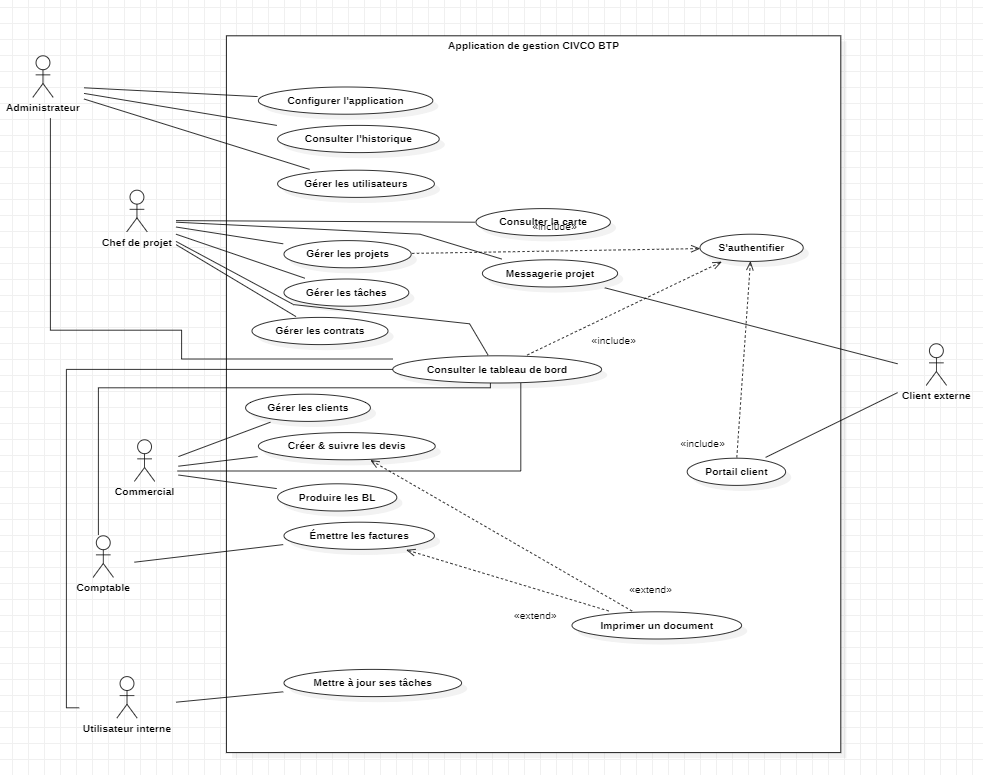
\includegraphics[width=\textwidth]{usecaseUML.png}
  \caption{Diagramme de cas d'utilisation de l'application CIVCO BTP}
  \label{fig:uc_diagram}
\end{figure}

\subsection{Diagramme de séquence}

Le diagramme de séquence (Figure~\ref{fig:seq_diagram}) illustre le scénario de création d'un devis par un
commercial. Les interactions mettent en évidence la séparation entre l'interface
React, l'API Laravel (validation, service métier) et la persistance en base de
données. Les étapes principales sont les suivantes :
\begin{enumerate}
  \item Le commercial s'authentifie via la SPA (cookie Sanctum + jeton CSRF).
  \item Il sélectionne un projet et saisit les lignes du devis.
  \item Le frontend envoie \texttt{POST /api/v1/quotes} avec les données JSON.
  \item Laravel valide la requête (Form Request), persiste le devis et ses lignes.
  \item L'API retourne une \texttt{QuoteResource} ; l'interface affiche la confirmation.
\end{enumerate}
Ce flux est représentatif du patron adopté sur l'ensemble des modules : le frontend
ne contient aucune logique métier critique ; la validation, les calculs et la
persistance sont toujours assurés côté serveur.

\medskip

D'autres scénarios de séquence ont été modélisés selon le même principe :
\textbf{conversion devis $\rightarrow$ facture} (contrôle du statut, transaction
base de données, copie des lignes), \textbf{signature de contrat} (génération
du PDF, capture de la signature canvas, mise à jour du statut) et
\textbf{assignation de tâche} (notification de l'utilisateur concerné).

\begin{figure}[H]
  \centering
  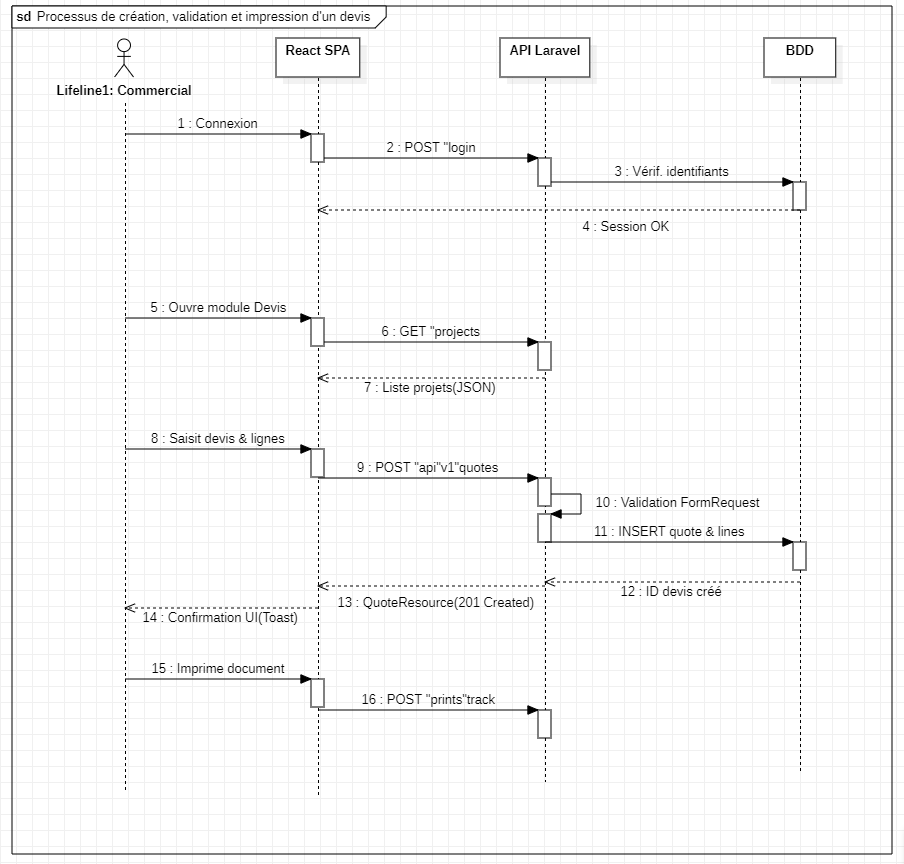
\includegraphics[width=\textwidth]{sequenceUML.png}
  \caption{Diagramme de séquence : création et enregistrement d'un devis}
  \label{fig:seq_diagram}
\end{figure}

\subsection{Diagramme de classes}

Le diagramme de classes (Figure~\ref{fig:class_diagram}) représente le modèle de données persistant simplifié.
Le Tableau~\ref{tab:classes} complète la description des entités principales et
de leurs relations.

\begin{figure}[H]
  \centering
  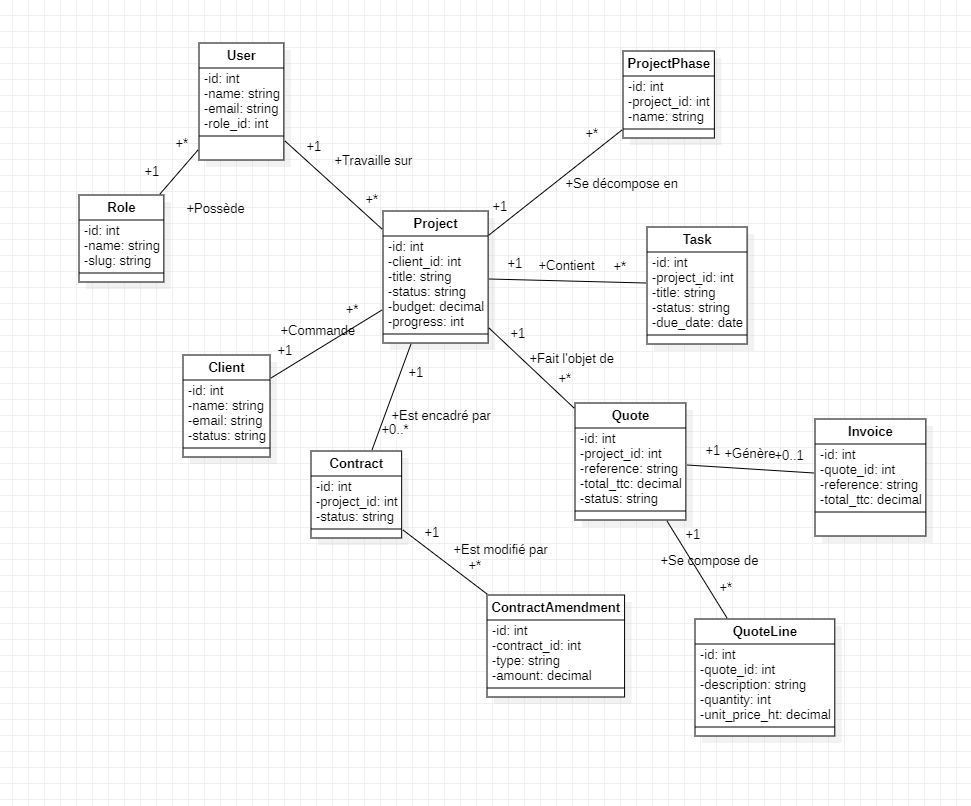
\includegraphics[width=\textwidth]{classeUML.png}
  \caption{Diagramme de classes simplifié du modèle de données métier}
  \label{fig:class_diagram}
\end{figure}

\begin{table}[H]
\caption{Description des classes et de leurs relations}
\label{tab:classes}
\centering
\small
\begin{tabular}{|l|p{4.8cm}|p{5.2cm}|}
\hline
\textbf{Classe} & \textbf{Attributs principaux} & \textbf{Relations} \\
\hline
\texttt{User} & id, name, email, role\_id & N User $\rightarrow$ 1 Role ;
N $\leftrightarrow$ N Project (équipe) \\
\hline
\texttt{Role} & id, name, slug & 1 Role $\rightarrow$ N Permission \\
\hline
\texttt{Client} & id, name, email, status & 1 Client $\rightarrow$ N Project ;
1 $\rightarrow$ N ClientContact \\
\hline
\texttt{Project} & id, client\_id, title, status, budget, progress & 1 $\rightarrow$ N Phase,
Task, Quote, Contract \\
\hline
\texttt{Quote} & id, project\_id, reference, total\_ttc, status & 1 $\rightarrow$ N QuoteLine ;
1 $\rightarrow$ 0..1 Invoice \\
\hline
\texttt{Invoice} & id, quote\_id, reference, total\_ttc & 1 $\rightarrow$ N InvoiceLine,
Payment \\
\hline
\texttt{Task} & id, project\_id, title, status, due\_date & N $\rightarrow$ 1 Project ;
N $\rightarrow$ 1 User (assigné) \\
\hline
\texttt{Contract} & id, project\_id, status & 1 $\rightarrow$ N ContractAmendment \\
\hline
\end{tabular}
\end{table}

\medskip

Le modèle met en évidence la \textbf{centralité du projet} : la plupart des entités
métier gravitent autour de \texttt{Project}, ce qui reflète l'organisation interne
de CIVCO BTP où le chantier constitue l'unité de travail de référence. Les
énumérations (\texttt{ProjectStatus}, \texttt{QuoteStatus}, \texttt{InvoiceStatus})
garantissent la cohérence des états dans l'application.

\subsection{Diagramme d'activité}

Le diagramme d'activité (Figure~\ref{fig:activity_diagram}) modélise le cycle de vie d'un projet de construction, depuis
sa création jusqu'à sa clôture. Le flux principal comprend : création du projet et
affectation du client, constitution de l'équipe et définition des phases, planification
des tâches, établissement du devis, signature du contrat, exécution des travaux avec
suivi d'avancement, facturation et clôture. Les points de décision portent sur
l'acceptation du devis et l'achèvement du projet ; en cas de refus, le devis peut
être révisé avant reprise du flux.

\vspace{0.4em}
\begin{center}
  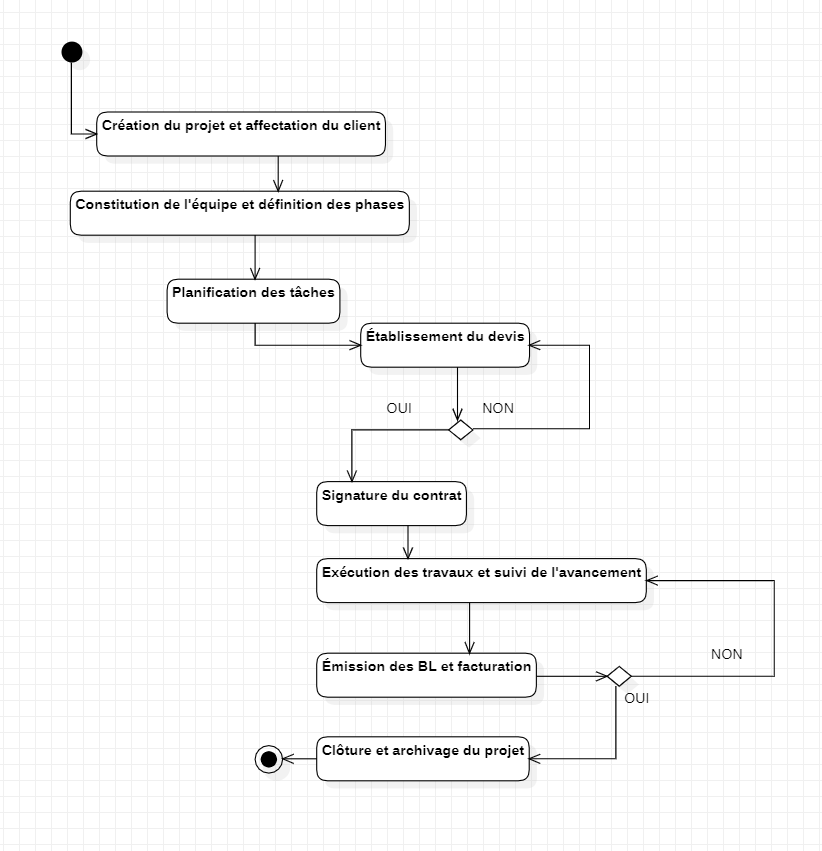
\includegraphics[height=0.50\textheight,keepaspectratio]{activiteUML.png}
  \captionof{figure}{Diagramme d'activité : cycle de vie d'un projet de construction}
  \label{fig:activity_diagram}
\end{center}

\newpage
\section*{Conclusion}

Ce chapitre a formalisé la conception de l'application de gestion de projets de
CIVCO BTP à travers trois niveaux d'abstraction complémentaires.

\medskip

Au niveau \textbf{fonctionnel}, l'analyse des besoins a identifié six acteurs métier,
vingt cas d'utilisation et treize exigences fonctionnelles couvrant l'ensemble du
cycle de vie d'un projet de construction : de la relation client à la facturation,
en passant par la planification des tâches et le suivi contractuel. Les neuf
exigences non-fonctionnelles fixent les contraintes de performance, de sécurité,
d'ergonomie et de maintenabilité auxquelles la solution doit répondre.

\medskip

Au niveau \textbf{architectural}, l'application repose sur une séparation nette en
trois couches : interface React en SPA, API Laravel exposant des services REST
sécurisés par Sanctum et RBAC, et persistance relationnelle via Eloquent. Le flux
d'authentification, la matrice des permissions et l'organisation modulaire du code
(backend par contrôleurs/services, frontend par features) garantissent une base
solide pour l'évolution future de l'outil.

\medskip

Au niveau \textbf{métier}, la conception détaillée des sept modules (projets, clients,
documents commerciaux, contrats, tâches, tableau de bord, portail client) traduit
les processus internes de CIVCO BTP en composants logiciels cohérents, avec des
règles de gestion explicites et des flux documentaires tracés.

\medskip

Enfin, la modélisation \textbf{UML} --- cas d'utilisation, séquence, classes et
activité --- formalise les interactions, le modèle de données et les flux métier,
et sert de référence pour la phase de réalisation décrite au chapitre suivant.

\medskip

Le chapitre suivant décrit l'implémentation concrète de cette conception : choix
d'environnement, structure du code, captures d'écran des modules principaux et
résultats de la campagne de tests.

\newpage

% \chapter{Réalisation et Implémentation}
\label{chap:realisation}

\section{Introduction}

Ce chapitre décrit la réalisation concrète de l'application de gestion et de planification
des projets BTP développée pour CIVCO BTP, à partir de la conception présentée au
chapitre précédent. Nous présentons d'abord l'environnement technique et les outils
utilisés, puis détaillons l'implémentation du backend Laravel, du frontend React et
des principaux modules métier. Le chapitre se conclut par les tests réalisés et les
résultats de validation.

% ─────────────────────────────────────────────────────────────────────
\section{Environnement technique}

\subsection{Stack technologique}

\begin{description}
  \item[Serveur applicatif] PHP 8.3, Laravel 13.8, Laravel Sanctum 4
  (authentification SPA), Eloquent ORM, migrations et seeders.
  \item[Interface utilisateur] React 19.2, Vite 8, React Router 7, Tailwind CSS 4, Axios,
  Recharts (graphiques), Leaflet (cartographie).
  \item[Base de données] MySQL / PostgreSQL (modèle relationnel,
  schéma versionné par migrations Laravel).
  \item[Outils complémentaires] Git / GitHub (versionnement), Visual Studio Code (IDE),
  PHPUnit 12 (tests backend), ESLint (qualité frontend).
\end{description}

Le Tableau~\ref{tab:stack_versions} récapitule les versions principales des composants
utilisés en développement.

\begin{table}[H]
\caption{Versions des composants de la stack technique}
\label{tab:stack_versions}
\centering
\small
\begin{tabular}{|l|l|p{6.5cm}|}
\hline
\textbf{Composant} & \textbf{Version} & \textbf{Rôle} \\
\hline
PHP & 8.3+ & Langage backend, exécution Laravel \\
\hline
Laravel & 13.8 & Framework API, ORM, authentification \\
\hline
Laravel Sanctum & 4.x & Sessions SPA sécurisées \\
\hline
React & 19.2 & Interface utilisateur composants \\
\hline
Vite & 8.0 & Build tool et serveur de développement \\
\hline
Tailwind CSS & 4.3 & Styles utilitaires \\
\hline
MySQL / PostgreSQL & 8.x / 16 & Persistance relationnelle \\
\hline
PHPUnit & 12.5 & Tests automatisés backend \\
\hline
\end{tabular}
\end{table}

\subsection{Outils de développement}

\begin{description}
  \item[Gestion de projet] Trello (tableau Kanban) pour planifier les modules,
  suivre l'avancement des tâches et préparer les démonstrations de suivi.
  \item[Contrôle de version] Git et GitHub pour le suivi des évolutions, branches de
  fonctionnalités et revues de code.
  \item[IDE] Visual Studio Code avec extensions PHP Intelephense, ESLint et Prettier.
  \item[Tests] PHPUnit pour les tests d'intégration API ; tests manuels sur navigateur
  (Chrome, Edge) pour les parcours utilisateurs.
  \item[Qualité de code] Laravel Pint (formatage PHP), ESLint (linting JavaScript/React).
  \item[Documentation API] Routes Laravel exposées sous \texttt{/api/v1/}, testables via
  outils HTTP (Postman, curl) ou le navigateur pour les endpoints GET.
\end{description}

\subsection{Architecture de déploiement}

\subsubsection{Environnement de développement}

En développement, l'application repose sur deux processus parallèles, orchestrés depuis
deux terminaux :

\begin{enumerate}
  \item \textbf{Backend Laravel} : \texttt{php artisan serve --host=127.0.0.1 --port=8000}
  expose l'API sur le port 8000.
  \item \textbf{Frontend Vite} : \texttt{npm run dev} lance le serveur de développement
  React sur le port 5173, avec rechargement à chaud (\textit{hot-reload}).
\end{enumerate}

Le fichier \texttt{vite.config.js} configure un proxy : les requêtes vers \texttt{/api},
\texttt{/sanctum} et \texttt{/storage} sont redirigées vers Laravel (port 8000), ce qui
évite les problèmes de CORS en développement et simule un déploiement unifié.

\subsubsection{Schéma de communication}

\begin{itemize}
  \item Le navigateur charge l'application React depuis \texttt{http://127.0.0.1:5173}.
  \item Les appels API transitent par le proxy Vite vers \texttt{http://127.0.0.1:8000/api/v1/}.
  \item Sanctum émet un cookie de session après authentification ; Axios est configuré
  avec \texttt{withCredentials: true}.
  \item Les fichiers uploadés (logos, documents, signatures) sont stockés dans
  \texttt{storage/app/public} et servis via le lien symbolique \texttt{public/storage}.
\end{itemize}

\subsubsection{Étude d'hébergement : OVHcloud vs o2switch}

En vue d'une mise en production chez CIVCO BTP, une \textbf{étude comparative
d'hébergement} a été menée entre deux prestataires français largement utilisés pour
les applications web PHP : \textbf{OVHcloud} et \textbf{o2switch}. L'objectif était
d'identifier la solution la mieux adaptée au profil de l'entreprise : application
métier interne, équipe réduite, budget maîtrisé et besoin de simplicité
d'administration.

\medskip

Les critères d'évaluation retenus sont les suivants :

\begin{itemize}
  \item \textbf{Compatibilité Laravel / PHP 8.3} : exécution de l'API backend et des
  commandes \texttt{artisan} (migrations, files d'attente, planificateur).
  \item \textbf{Base de données} : support MySQL ou PostgreSQL, sauvegardes et quotas.
  \item \textbf{Déploiement du frontend React} : hébergement des fichiers statiques
  produits par \texttt{npm run build}.
  \item \textbf{Sécurité} : certificat SSL, pare-feu, mises à jour système.
  \item \textbf{Coût et prévisibilité} : tarification mensuelle, absence de surprises
  sur la facturation.
  \item \textbf{Support et localisation} : assistance en français, datacenters en
  France, conformité pour des données clients BTP.
  \item \textbf{Facilité d'exploitation} : courbe d'apprentissage pour une PME sans
  équipe DevOps dédiée.
\end{itemize}

\begin{table}[H]
\caption{Comparatif d'hébergement : OVHcloud vs o2switch}
\label{tab:hebergement}
\centering
\small
\begin{tabular}{|p{3.2cm}|p{5.2cm}|p{5.2cm}|}
\hline
\textbf{Critère} & \textbf{OVHcloud} & \textbf{o2switch} \\
\hline
Type d'offre & VPS, cloud public, serveurs dédiés (IaaS) & Hébergement mutualisé
tout-en-un \\
\hline
Laravel / PHP & Compatible (configuration manuelle : Nginx, PHP-FPM, Composer) &
Compatible nativement (PHP 8.x, SSH, Composer) \\
\hline
Base de données & MySQL/PostgreSQL à installer et administrer & MySQL inclus,
bases multiples \\
\hline
Frontend React (build) & Fichiers statiques sur VPS ou Object Storage & Hébergement
direct des assets \texttt{dist/} \\
\hline
SSL (HTTPS) & Let's Encrypt ou certificat payant (selon offre) & Let's Encrypt
inclus et automatisé \\
\hline
Sauvegardes & À configurer (snapshots, scripts) & Sauvegardes journalières incluses \\
\hline
Tarification & Variable (facturation à l'usage, snapshots, trafic) & Forfait fixe
illimité (offre unique) \\
\hline
Support & Tickets, documentation technique & Support français réactif, panel cPanel \\
\hline
Scalabilité & Élevée (montée en charge horizontale) & Modérée (mutualisé, adapté PME) \\
\hline
Complexité admin & Élevée (sysadmin requis) & Faible (panel graphique) \\
\hline
\end{tabular}
\end{table}

\medskip

\textbf{Analyse.} OVHcloud~\cite{ovhcloud} offre une grande flexibilité et une
scalabilité adaptée aux applications à fort trafic ou aux architectures distribuées
(conteneurs Docker, load balancing, bases managées). En revanche, le déploiement d'une
application Laravel + React sur un VPS OVHcloud suppose une configuration manuelle
du serveur web, de PHP-FPM, des certificats, des sauvegardes et de la supervision.
Cette approche est pertinente pour des équipes disposant de compétences
d'administration système, mais elle représente un surcoût en temps pour une PME comme
CIVCO BTP.

\medskip

o2switch~\cite{o2switch}, hébergeur français basé à Grabels, propose une offre
mutualisée orientée simplicité : PHP récent, bases MySQL, certificats SSL gratuits,
sauvegardes automatiques et support technique francophone. Pour une application métier
interne au volume d'utilisateurs modéré (équipes CIVCO BTP et clients portail), cette
formule couvre les besoins sans nécessiter la gestion d'un serveur virtuel. Le frontend
React est déployé sous forme de fichiers statiques (\texttt{npm run build}), tandis que
Laravel gère l'API et les sessions Sanctum sur le même domaine, simplifiant la
configuration des cookies et du CSRF.

\medskip

\textbf{Choix retenu.} Au terme de cette étude, \textbf{o2switch} a été retenu comme
plateforme d'hébergement cible pour CIVCO BTP. Ce choix se justifie par :

\begin{itemize}
  \item un \textbf{rapport qualité/prix} favorable pour une application interne ;
  \item une \textbf{mise en production plus rapide}, sans administration système
  avancée ;
  \item une \textbf{compatibilité native} avec la stack Laravel / MySQL ;
  \item un \textbf{support en français} et des datacenters localisés en France ;
  \item des \textbf{sauvegardes et SSL inclus}, répondant aux exigences de sécurité
  identifiées au Chapitre~3.
\end{itemize}

OVHcloud reste une alternative crédible si l'application devait évoluer vers une
architecture plus complexe (montée en charge importante, microservices, conteneurisation
Docker). Pour la première version de l'outil, la simplicité opérationnelle d'o2switch
a été privilégiée.

\subsubsection{Configuration : variables d'environnement}

La configuration sensible est centralisée dans le fichier \texttt{.env} du backend.
Le Tableau~\ref{tab:env_vars} liste les variables principales :

\begin{table}[H]
\caption{Variables d'environnement principales du fichier \texttt{.env}}
\label{tab:env_vars}
\centering
\small
\begin{tabular}{|l|p{7.5cm}|}
\hline
\textbf{Variable} & \textbf{Rôle} \\
\hline
\texttt{APP\_URL} & URL publique de l'application (ex. \texttt{http://127.0.0.1:8000}) \\
\hline
\texttt{DB\_CONNECTION / DB\_DATABASE} & Connexion SGBD (MySQL ou PostgreSQL) \\
\hline
\texttt{SESSION\_DRIVER} & Pilote de session (fichier ou base de données) \\
\hline
\texttt{SANCTUM\_STATEFUL\_DOMAINS} & Domaines autorisés pour les cookies Sanctum \\
\hline
\texttt{FRONTEND\_URL} & URL du frontend (pour les redirections et CORS) \\
\hline
\texttt{MAIL\_*} & Configuration SMTP (notifications, invitations portail) \\
\hline
\end{tabular}
\end{table}

\subsubsection{Initialisation de la base de données}

Le démarrage d'un environnement neuf suit la séquence standard Laravel :

\begin{enumerate}
  \item \texttt{composer install} : installation des dépendances PHP.
  \item \texttt{cp .env.example .env} puis configuration de la base de données.
  \item \texttt{php artisan key:generate} : génération de la clé d'application.
  \item \texttt{php artisan migrate --seed} : création du schéma et données de démonstration.
  \item \texttt{php artisan storage:link} : lien symbolique pour les fichiers publics.
\end{enumerate}

Les seeders (\texttt{DatabaseSeeder}, \texttt{DemoSeeder}, \texttt{RoleSeeder}) peuplent
la base avec des utilisateurs de test, des rôles, des permissions, des clients et des
projets représentatifs du secteur BTP au Maroc.

% ─────────────────────────────────────────────────────────────────────
\section{Implémentation du backend}

\subsection{Structure du projet}

Le backend suit l'architecture modulaire Laravel, organisée par responsabilité :

\begin{verbatim}
backend/
+-- app/
|   +-- Enums/              # Statuts (Project, Quote, Invoice, Client...)
|   +-- Http/
|   |   +-- Controllers/Api/V1/   # ~45 controleurs REST
|   |   +-- Middleware/           # Auth, permissions, contexte
|   |   +-- Requests/             # Validation par domaine
|   |   +-- Resources/            # Serialisation JSON
|   +-- Models/             # Entites Eloquent (~35 modeles)
|   +-- Services/           # Logique metier (QuoteService, etc.)
+-- database/
|   +-- migrations/         # ~70 migrations versionnees
|   +-- seeders/            # Donnees de demo et referentiels
+-- routes/api.php          # Definition des routes /api/v1/
\-- tests/Feature/          # Tests PHPUnit d'integration
\end{verbatim}

Cette organisation sépare clairement le transport HTTP (contrôleurs), la validation
(Requests), la transformation des réponses (Resources) et la logique métier (Services),
conformément au patron décrit au Chapitre~3.

\subsection{API REST : endpoints principaux}

L'API est regroupée sous le préfixe \texttt{/api/v1/}. Les endpoints principaux sont
organisés par domaine fonctionnel :

\begin{description}
  \item[Authentification] \texttt{POST /login}, \texttt{GET /me}, \texttt{POST /logout},
  \texttt{PATCH /me} (profil utilisateur). Gestion de session via Sanctum.
  \item[Projets] \texttt{GET/POST /projects}, \texttt{GET/PATCH/DELETE /projects/\{id\}},
  gestion des phases, équipe, dépenses, médias et commentaires.
  \item[Clients] \texttt{GET/POST /clients}, archivage, contacts, provisionnement
  portail (\texttt{POST /clients/\{id\}/portal-account}).
  \item[Devis] \texttt{GET/POST /quotes}, lignes de détail, conversion en facture,
  suivi des statuts et impressions.
  \item[Factures] \texttt{GET/POST /invoices}, paiements, état de facturation.
  \item[Bons de livraison] \texttt{GET/POST /delivery-forms}, lignes et statuts.
  \item[Contrats] \texttt{GET/POST /contracts}, compilation, signature, avenants
  (\texttt{/contract-amendments}).
  \item[Tâches] \texttt{GET/POST /tasks}, assignation, filtrage par projet et utilisateur.
  \item[Équipe] \texttt{GET /team/members}, gestion des membres et rôles.
  \item[Configuration] \texttt{/roles}, \texttt{/document-templates},
  \texttt{/tenant/document-controls}, thème et badges.
  \item[Tableau de bord] \texttt{GET /dashboard/summary}, indicateurs agrégés.
  \item[Recherche] \texttt{GET /search}, recherche globale multi-entités.
  \item[Portail client] \texttt{/client-portal/*} : projets, devis, contrats,
  messagerie, acceptation et signature.
  \item[Historique] \texttt{GET /activity-logs}, journal des actions.
\end{description}

Chaque route métier sensible est protégée par le middleware \texttt{permission:*},
qui vérifie que l'utilisateur authentifié dispose du droit requis avant d'exécuter
l'action.

\subsection{Services métier}

La logique complexe est extraite des contrôleurs vers des classes Service :

\begin{itemize}
  \item \textbf{QuoteService / InvoiceService} : calcul des totaux, numérotation,
  conversion devis $\rightarrow$ facture, gestion des statuts.
  \item \textbf{DeliveryFormService} : production des bons de livraison et liaison
  aux projets.
  \item \textbf{DocumentService / DocumentTemplateCompilationService} : génération
  et compilation des documents à partir de modèles.
  \item \textbf{DashboardService} : agrégation des indicateurs (projets actifs,
  tâches en retard, chiffre d'affaires).
  \item \textbf{AuthContextService} : résolution du contexte utilisateur (rôles,
  permissions, société courante).
  \item \textbf{ActivityLogService} : journalisation des actions sensibles.
  \item \textbf{PrintTrackingService} : suivi des impressions officielles et quotas.
  \item \textbf{SiteGeocodingService} : géolocalisation des chantiers (Nominatim +
  coordonnées de repli pour les villes marocaines).
\end{itemize}

\subsection{Authentification et contrôle d'accès}

L'authentification repose sur \textbf{Laravel Sanctum} en mode SPA :

\begin{enumerate}
  \item Le frontend obtient un cookie CSRF via \texttt{GET /sanctum/csrf-cookie}.
  \item L'utilisateur envoie ses identifiants à \texttt{POST /api/v1/login}.
  \item Laravel valide, crée une session et retourne le profil (\texttt{UserResource})
  avec rôles et permissions.
  \item Chaque requête ultérieure inclut le cookie de session ; le middleware
  \texttt{auth:sanctum} protège les routes.
  \item Le middleware \texttt{permission:slug} vérifie les droits granulaires
  (\texttt{project.view}, \texttt{quote.manage}, etc.).
\end{enumerate}

Le service \texttt{PostLoginRedirectService} oriente l'utilisateur vers la page
d'accueil adaptée à son profil (tableau de bord admin, liste des projets pour un
chef de projet, factures pour un comptable).

\subsection{Migrations et modèle de données}

Le schéma de base compte environ 70 migrations, couvrant l'ensemble des entités métier.
Les migrations sont idempotentes et versionnées : chaque modification de schéma
produit un nouveau fichier daté, exécutable de façon reproductible sur tout
environnement.

\medskip

Les relations Eloquent principales ont été implémentées comme suit :
\begin{itemize}
  \item \texttt{Client} \texttt{hasMany} \texttt{Project}
  \item \texttt{Project} \texttt{belongsTo} \texttt{Client}, \texttt{hasMany} \texttt{ProjectPhase},
  \texttt{Task}, \texttt{Quote}, \texttt{Contract}
  \item \texttt{Quote} \texttt{hasMany} \texttt{QuoteLine}, \texttt{hasOne} \texttt{Invoice}
  \item \texttt{User} \texttt{belongsToMany} \texttt{Project} (équipe), \texttt{belongsTo} \texttt{Role}
\end{itemize}

Les \textbf{API Resources} (\texttt{ProjectResource}, \texttt{QuoteResource}, etc.)
contrôlent les champs exposés au frontend et permettent d'inclure conditionnellement
les relations (\texttt{client}, \texttt{lines}, \texttt{teamMembers}).

\subsection{Middleware et sécurité des routes}

Le pipeline de middleware Laravel applique une chaîne de vérifications sur chaque
requête API protégée :

\begin{enumerate}
  \item \textbf{auth:sanctum} : vérifie que l'utilisateur est authentifié via session.
  \item \textbf{EnsureCompanyContext} : résout la société courante à partir de
  l'en-tête \texttt{X-Company-Id} ou du contexte utilisateur.
  \item \textbf{permission:slug} : contrôle granulaire par action métier
  (\texttt{client.view}, \texttt{invoice.manage}, etc.).
  \item \textbf{ValidateCsrfToken} : protection contre les requêtes forgées sur
  les verbes mutants (\texttt{POST}, \texttt{PUT}, \texttt{PATCH}, \texttt{DELETE}).
\end{enumerate}

Cette approche en profondeur (\textit{defense in depth}) garantit qu'aucune action
métier ne peut être exécutée sans authentification et sans autorisation explicite,
conformément aux bonnes pratiques de sécurité web~\cite{owasp}.

\subsection{Exemple : création d'un devis}

Le flux de création d'un devis illustre l'interaction entre les couches :

\begin{enumerate}
  \item Le frontend envoie \texttt{POST /api/v1/quotes} avec le corps JSON
  (client, projet, lignes, montants).
  \item \texttt{StoreQuoteRequest} valide les champs (références obligatoires,
  montants positifs, dates cohérentes).
  \item \texttt{QuoteController@store} délègue à \texttt{QuoteService::create()}.
  \item Le service crée l'enregistrement \texttt{Quote} et ses \texttt{QuoteLine}
  associées dans une transaction base de données.
  \item Les totaux HT, TVA et TTC sont calculés automatiquement.
  \item \texttt{QuoteResource} sérialise la réponse JSON pour le frontend.
  \item \texttt{ActivityLogService} journalise l'action si configuré.
\end{enumerate}

Ce patron (Request $\rightarrow$ Controller $\rightarrow$ Service $\rightarrow$
Resource) est reproduit sur l'ensemble des modules métier.

\subsection{Modules complémentaires}

En complément des modules principaux, plusieurs fonctionnalités transverses ont été
implémentées :

\medskip

\textbf{Notifications :} le modèle \texttt{Notification} et le contrôleur associé
permettent d'informer les utilisateurs des événements importants (nouvelle tâche
assignée, devis accepté, message reçu). L'interface affiche un badge de notification
non lue dans l'en-tête.

\medskip

\textbf{Messagerie :} le module \texttt{PortalMessage} gère les échanges entre
l'équipe interne et les clients externes, scopés par projet. Le service
\texttt{PortalMessageService} filtre les conversations selon les droits de
l'utilisateur (\texttt{can\_chat\_with\_client} sur les membres d'équipe).

\medskip

\textbf{Recherche globale :} le composant \texttt{GlobalSearch} et l'endpoint
\texttt{GET /search} permettent de retrouver rapidement un client, un projet, un
devis ou une facture par mot-clé, améliorant la productivité au quotidien.

\medskip

\textbf{Contrôle d'impression :} \texttt{PrintTrackingService} gère les quotas
d'impressions officielles par type de document et par en-tête (avec ou sans papier
à en-tête). Au-delà du quota, les impressions sont marquées « COPIE - NON OFFICIEL ».

\medskip

\textbf{Journal d'activité :} chaque action sensible (création de projet, validation
de devis, archivage client) est enregistrée par \texttt{ActivityLogService} avec
l'identité de l'utilisateur, le type d'action et l'horodatage. Le module
\texttt{features/history/} expose ces entrées sous forme de fil d'audit consultable
par l'administrateur.

\medskip

\textbf{Géocodage des chantiers :} lors de la saisie d'une adresse de chantier,
\texttt{SiteGeocodingService} tente de résoudre automatiquement les coordonnées
GPS via l'API Nominatim (OpenStreetMap). En cas d'échec, un référentiel de
coordonnées des principales villes marocaines (\texttt{MoroccoCityCoordinates})
assure un positionnement approximatif sur la carte Leaflet.

\medskip

\textbf{Modèles de documents :} le module \texttt{DocumentTemplate} permet de
définir des gabarits de contrats et de documents commerciaux avec des champs
dynamiques (placeholders). Le service \texttt{DocumentTemplateCompilationService}
injecte les données du projet et du client lors de la génération du document final.

\medskip

\textbf{Gestion d'équipe :} \texttt{TeamMemberService} et \texttt{TeamQueryService}
centralisent l'affectation des collaborateurs aux projets, la gestion des rôles
sur chantier et le contrôle de l'autorisation de messagerie client
(\texttt{can\_chat\_with\_client}).

% ─────────────────────────────────────────────────────────────────────
\section{Implémentation du frontend}

\subsection{Architecture React}

Le frontend est une SPA React 19 organisée par domaines métier (\textit{features}) :

\begin{verbatim}
frontend/src/
+-- api/                    # Modules Axios par ressource
|   +-- client.js           # Instance Axios + intercepteurs
|   +-- projects.js, clients.js, quotes.js, invoices.js...
+-- components/             # Composants transverses (Sidebar, Modal...)
+-- context/
|   +-- AuthContext.jsx     # Session, roles, permissions
|   +-- ThemeContext.jsx    # Theme sombre, couleurs societe
|   +-- LanguageContext.jsx # i18n FR / EN
+-- features/
|   +-- dashboard/          # Tableau de bord et widgets
|   +-- projects/           # Liste, detail, phases, equipe
|   +-- clients/            # Gestion clients et portail
|   +-- quotes/             # Devis
|   +-- invoices/           # Factures
|   +-- delivery-forms/     # Bons de livraison
|   +-- tasks/              # Taches
|   +-- configuration/      # Parametres, roles, modeles
|   +-- profile/            # Profil utilisateur
+-- routes/
|   +-- AppRoutes.jsx       # Definition des routes
|   +-- routePermissions.js # Controle d'acces par route
\-- i18n/locales/           # Traductions fr.js, en.js
\end{verbatim}

\subsection{Client HTTP et authentification}

Le module \texttt{api/client.js} centralise la configuration Axios :

\begin{itemize}
  \item \texttt{baseURL} pointant vers \texttt{/api/v1} (proxifié par Vite).
  \item \texttt{withCredentials: true} pour transmettre les cookies Sanctum.
  \item Intercepteur de requête : récupération du jeton CSRF depuis le cookie
  \texttt{XSRF-TOKEN} et injection dans l'en-tête \texttt{X-XSRF-TOKEN}.
  \item Intercepteur de réponse : redirection vers \texttt{/login} en cas de
  \texttt{401 Unauthorized}.
  \item En-tête \texttt{X-Company-Id} pour le contexte société lorsque requis.
\end{itemize}

Le \texttt{AuthContext} expose l'état global d'authentification : utilisateur courant,
rôles, permissions, fonctions \texttt{login} / \texttt{logout}, et helpers de
vérification des droits consommés par les composants \texttt{PermissionGate} et
\texttt{AdminRoute}.

\subsection{Routage et contrôle d'accès}

\texttt{AppRoutes.jsx} définit l'arborescence de navigation :

\begin{itemize}
  \item Routes publiques : \texttt{/login}.
  \item Routes authentifiées : \texttt{/} (dashboard), \texttt{/projects},
  \texttt{/clients}, \texttt{/quotes}, \texttt{/invoices}, \texttt{/tasks},
  \texttt{/map}, \texttt{/configuration}, \texttt{/history}.
  \item Portail client : \texttt{/portal/*} (interface dédiée aux clients externes).
  \item Protection : composants \texttt{ProtectedRoute}, \texttt{AdminRoute} et
  fonction \texttt{canAccessRoute()} qui croise le chemin demandé avec les
  permissions de l'utilisateur.
\end{itemize}

\subsection{Composants transverses}

Plusieurs composants partagés structurent l'expérience utilisateur :

\begin{itemize}
  \item \textbf{Sidebar} : navigation principale, filtrée selon les permissions.
  \item \textbf{AppLayout} : enveloppe commune (sidebar + en-tête + contenu).
  \item \textbf{GlobalSearch} : recherche unifiée clients, projets, documents.
  \item \textbf{CommercialPrintSheet} : génération et impression des documents
  commerciaux (devis, factures, BL) avec suivi des impressions.
  \item \textbf{PrintOptionsModal} : choix d'impression (avec/sans en-tête,
  copie officielle).
\end{itemize}

\subsection{Internationalisation}

L'application supporte le français (par défaut) et l'anglais via \texttt{LanguageContext}
et les fichiers \texttt{i18n/locales/fr.js} et \texttt{en.js}. Les libellés de
l'interface, les messages d'erreur et les intitulés de menus sont externalisés,
facilitant l'ajout de nouvelles langues.

\subsection{Détail des modules frontend}

Chaque module \textit{feature} suit une structure cohérente : une page liste
(\texttt{*Page.jsx}), une ou plusieurs pages détail (\texttt{*DetailPage.jsx}),
des composants locaux (\texttt{components/}) et un module API dédié
(\texttt{api/*.js}).

\medskip

\textbf{Module Projets} (\texttt{features/projects/}) : \texttt{ProjectsPage} affiche
la liste filtrable des chantiers ; \texttt{ProjectDetailPage} regroupe les onglets
phases, tâches, équipe, documents et contrats. Le composant \texttt{ProjectAmendmentsTab}
gère les avenants contractuels.

\medskip

\textbf{Module Clients} (\texttt{features/clients/}) : \texttt{ClientsPage} avec
recherche et filtres ; \texttt{NewClientModal} pour la création ; \texttt{ClientPortalPanel}
pour la gestion de l'accès portail. Le composant \texttt{ConfirmArchiveModal} sécurise
l'archivage.

\medskip

\textbf{Module Documents commerciaux} : \texttt{QuotesPage}, \texttt{QuoteDetailPage},
\texttt{InvoicesPage}, \texttt{DeliveryFormDetailPage}. Les composants d'impression
(\texttt{CommercialPrintSheet}, \texttt{DeliveryFormPrintSheet}) génèrent les
versions PDF imprimables.

\medskip

\textbf{Module Configuration} (\texttt{features/configuration/}) : panneaux dédiés
pour les rôles (\texttt{RolesSettingsPanel}), les modèles de contrats
(\texttt{ContractTemplateSettingsPanel}), les contrôles d'impression
(\texttt{DocumentControlsSettingsPanel}) et les modèles de documents
(\texttt{DocumentTemplatesSettingsPanel}).

\subsection{Gestion d'état et hooks}

L'état applicatif repose principalement sur React Context :

\begin{itemize}
  \item \textbf{AuthContext} : session utilisateur, permissions, fonctions login/logout.
  \item \textbf{ThemeContext} : couleurs de la société injectées en variables CSS.
  \item \textbf{LanguageContext} : bascule FR / EN de l'interface.
  \item \textbf{usePolicyPrint / useProjectTasks} : hooks métier encapsulant la
  logique d'impression et de chargement des tâches projet.
\end{itemize}

React Query (\texttt{@tanstack/react-query}) est installé et prêt pour le cache
des requêtes API ; son adoption progressive permettra d'optimiser les rechargements
de listes et fiches détail.

% ─────────────────────────────────────────────────────────────────────
\section{Déroulement du développement et livrables}

\subsection{Phases de réalisation}

Le développement a suivi la planification définie au Chapitre~1, avec une
progression par modules fonctionnels. Chaque phase a produit un incrément
démontrable lors des réunions de suivi hebdomadaires avec l'encadrant professionnel.

\begin{table}[H]
\caption{Phases de développement et modules livrés}
\label{tab:livrables}
\centering
\small
\begin{tabular}{|l|p{5.5cm}|p{5.5cm}|}
\hline
\textbf{Phase} & \textbf{Modules livrés} & \textbf{Validation} \\
\hline
Fondations & Auth Sanctum, RBAC, navigation React, layout & Connexion multi-profils \\
\hline
Cœur métier & Projets, clients, phases, équipe & CRUD complet, carte \\
\hline
Documents & Devis, factures, BL, impression & Cycle commercial bout en bout \\
\hline
Opérations & Tâches, contrats, avenants, dépenses & Suivi opérationnel \\
\hline
Collaboration & Portail client, messagerie, notifications & Parcours client externe \\
\hline
Gouvernance & Configuration, historique, recherche globale & Administration complète \\
\hline
\end{tabular}
\end{table}

\subsection{Synthèse quantitative des livrables}

Au terme du stage, l'application comprend les éléments quantitatifs suivants,
illustrant l'ampleur de la réalisation :

\begin{itemize}
  \item Plus de \textbf{70 migrations} de base de données versionnées.
  \item Environ \textbf{40 contrôleurs API} et \textbf{25 services métier}.
  \item Plus de \textbf{30 modules frontend} (\textit{features} et composants).
  \item Une suite de \textbf{7 classes de tests} PHPUnit couvrant les flux critiques.
  \item Plus de \textbf{200 routes API} protégées par middleware d'authentification
  et de permissions.
  \item Support \textbf{bilingue} (français / anglais) sur l'ensemble de l'interface.
\end{itemize}

\subsection{Bonnes pratiques adoptées}

Plusieurs bonnes pratiques de génie logiciel ont été appliquées tout au long du
développement :

\begin{itemize}
  \item \textbf{Séparation des responsabilités} : contrôleurs fins, logique métier
  dans les services, validation dans les Form Requests.
  \item \textbf{Conventions de nommage} : respect des standards Laravel (PascalCase
  pour les classes, snake\_case pour les colonnes) et React (PascalCase pour les
  composants).
  \item \textbf{Versionnement Git} : branches par fonctionnalité, commits atomiques,
  messages descriptifs.
  \item \textbf{Suivi Kanban (Trello)} : chaque module ou correction était modélisé
  sous forme de carte, déplacée au fil de l'avancement entre les colonnes du tableau.
  \item \textbf{Revue de code} : validation des choix techniques avec l'encadrant
  professionnel avant intégration des modules sensibles (facturation, permissions).
  \item \textbf{Documentation inline} : commentaires sur les règles métier non
  évidentes, docblocks sur les méthodes de service exposées à l'API.
\end{itemize}

% ─────────────────────────────────────────────────────────────────────
\section{Interfaces principales}

Cette section présente les écrans clés de l'application. Les captures d'écran seront
insérées ultérieurement ; les descriptions ci-dessous reflètent l'implémentation
actuelle.

\subsection{Page de connexion}

\begin{figure}[H]
  \centering
  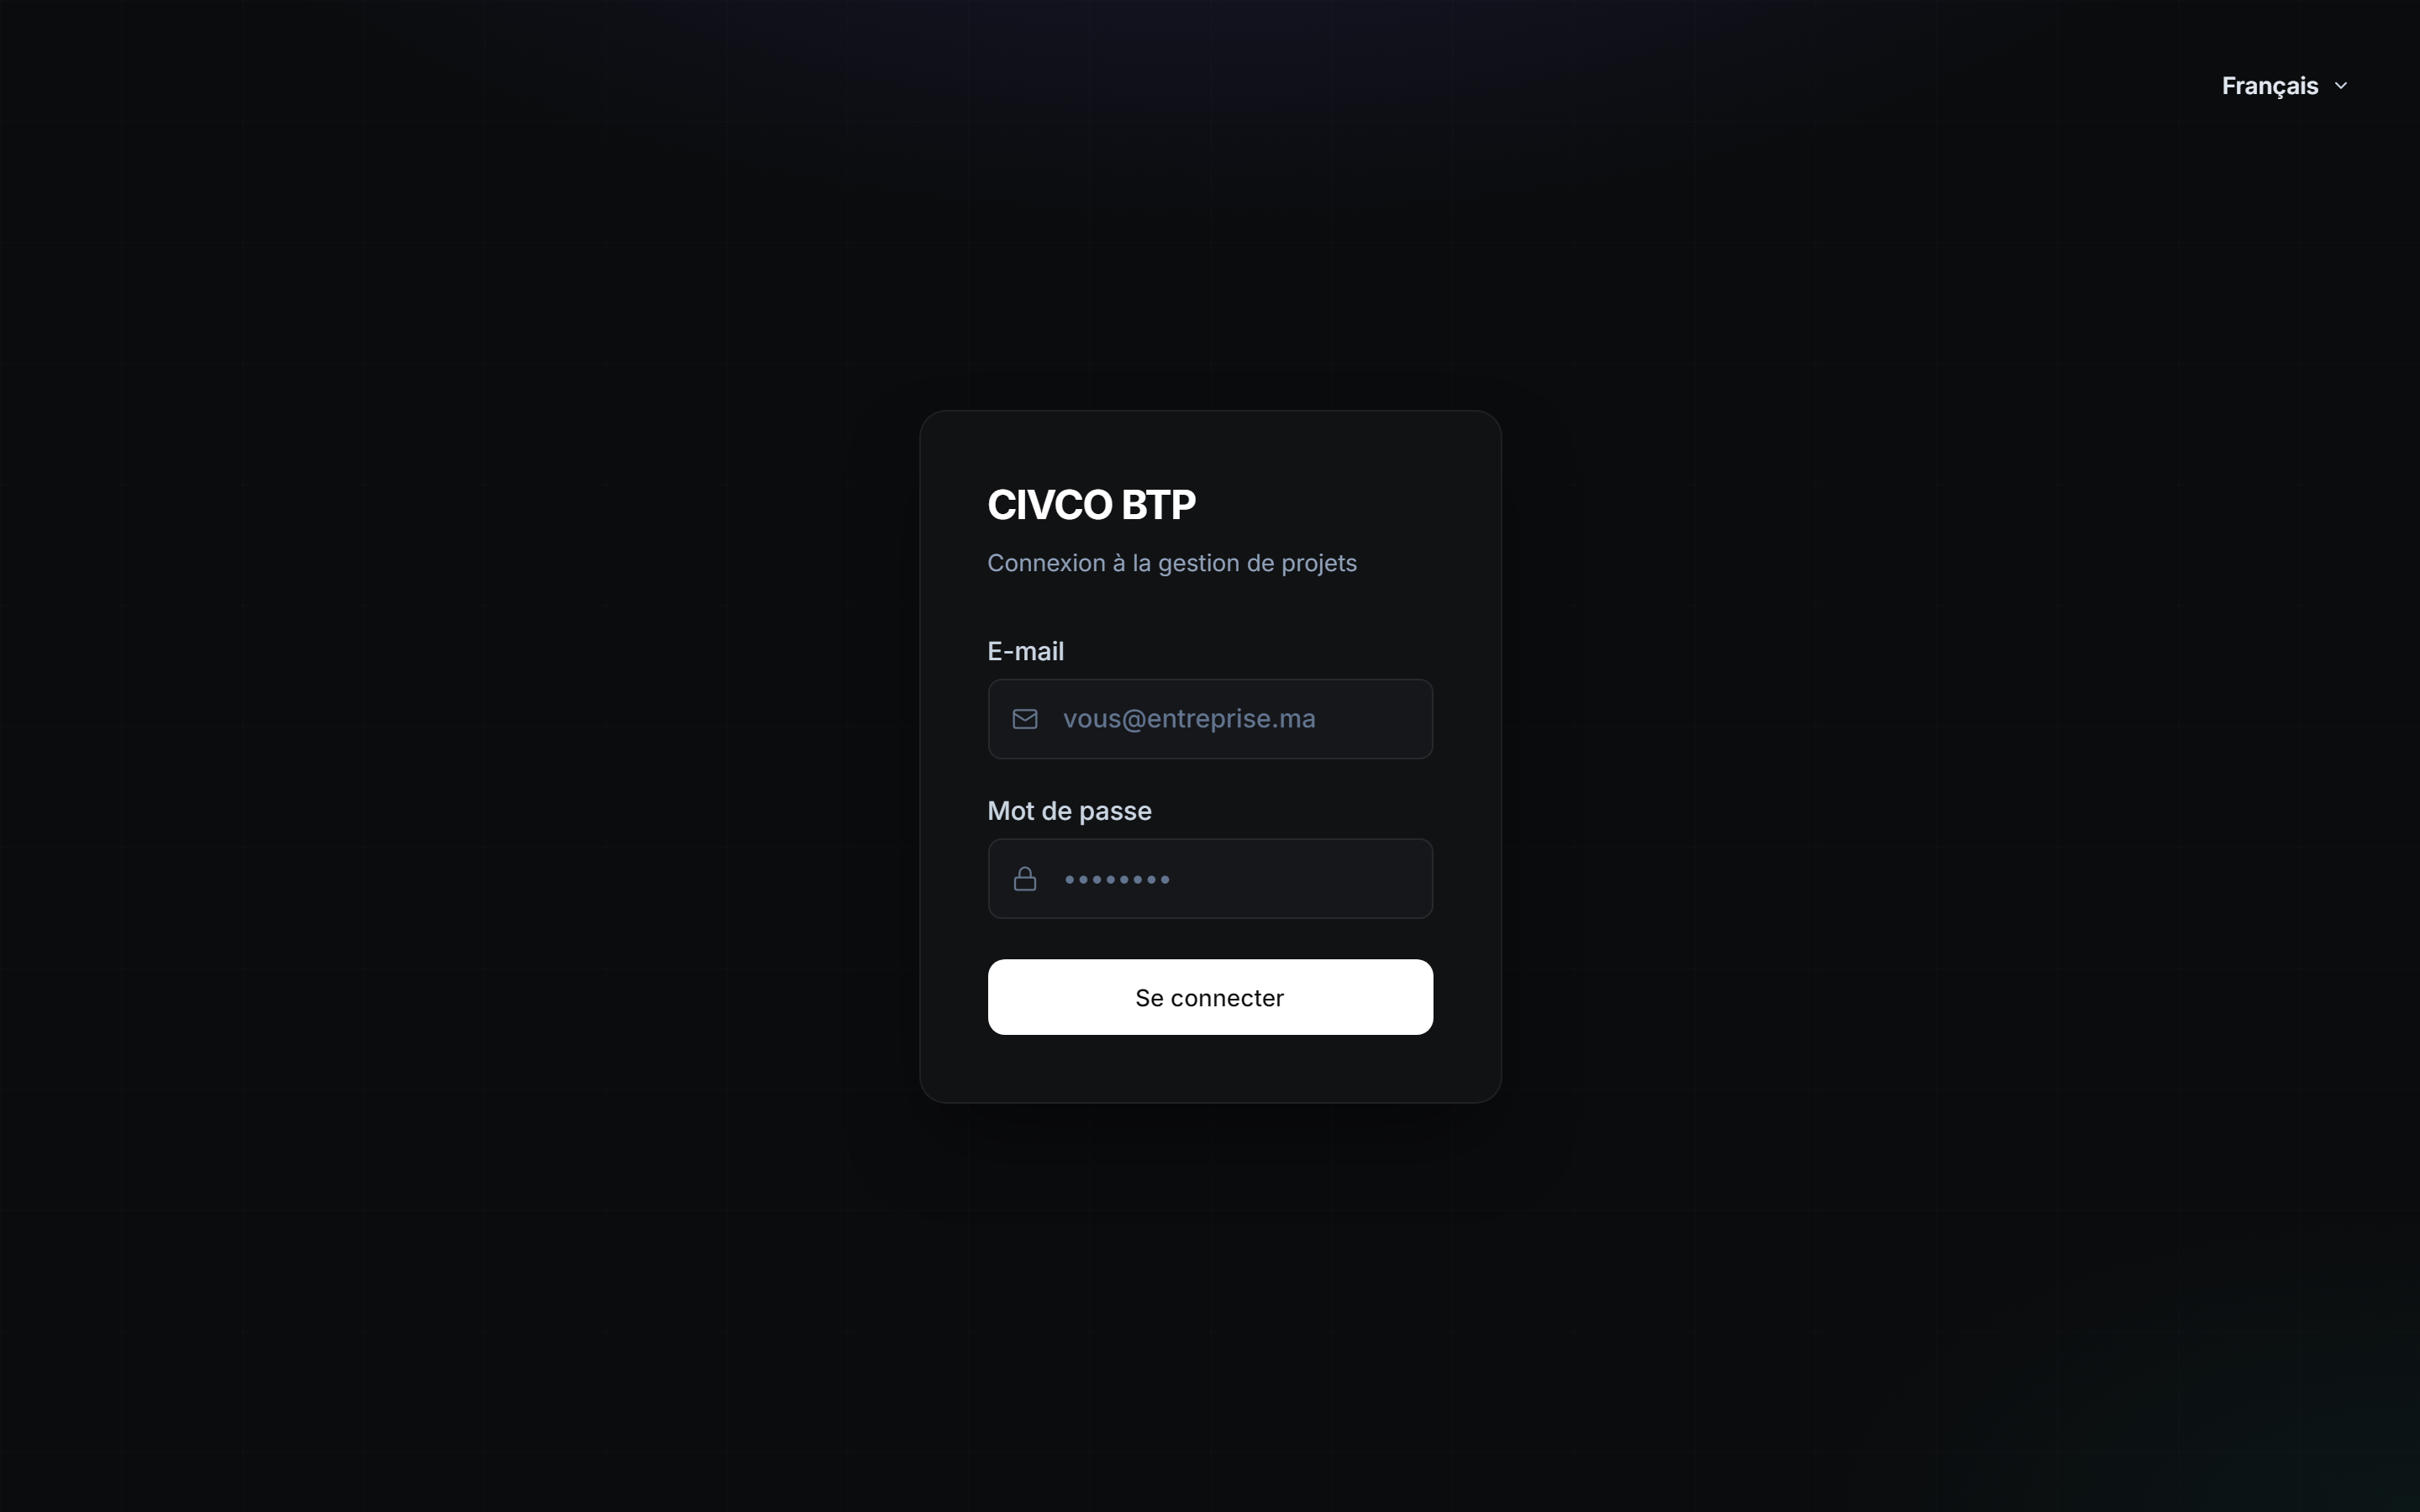
\includegraphics[width=\textwidth]{login.png}
  \caption{Page de connexion : authentification par email et mot de passe}
  \label{fig:login}
\end{figure}

La page de connexion (Figure~\ref{fig:login}) permet à tout utilisateur interne de
CIVCO BTP de s'authentifier. Après validation, l'utilisateur est redirigé vers la
page d'accueil correspondant à son profil métier.

\medskip

L'écran affiche le logo de l'entreprise, un formulaire email/mot de passe et une
option « Se souvenir de moi ». Les erreurs d'authentification (identifiants
incorrects, compte désactivé) sont affichées de manière explicite. Le design sombre
et épuré a été choisi pour réduire la fatigue visuelle lors d'une utilisation
quotidienne prolongée.

\subsection{Tableau de bord}

\begin{figure}[H]
  \centering
  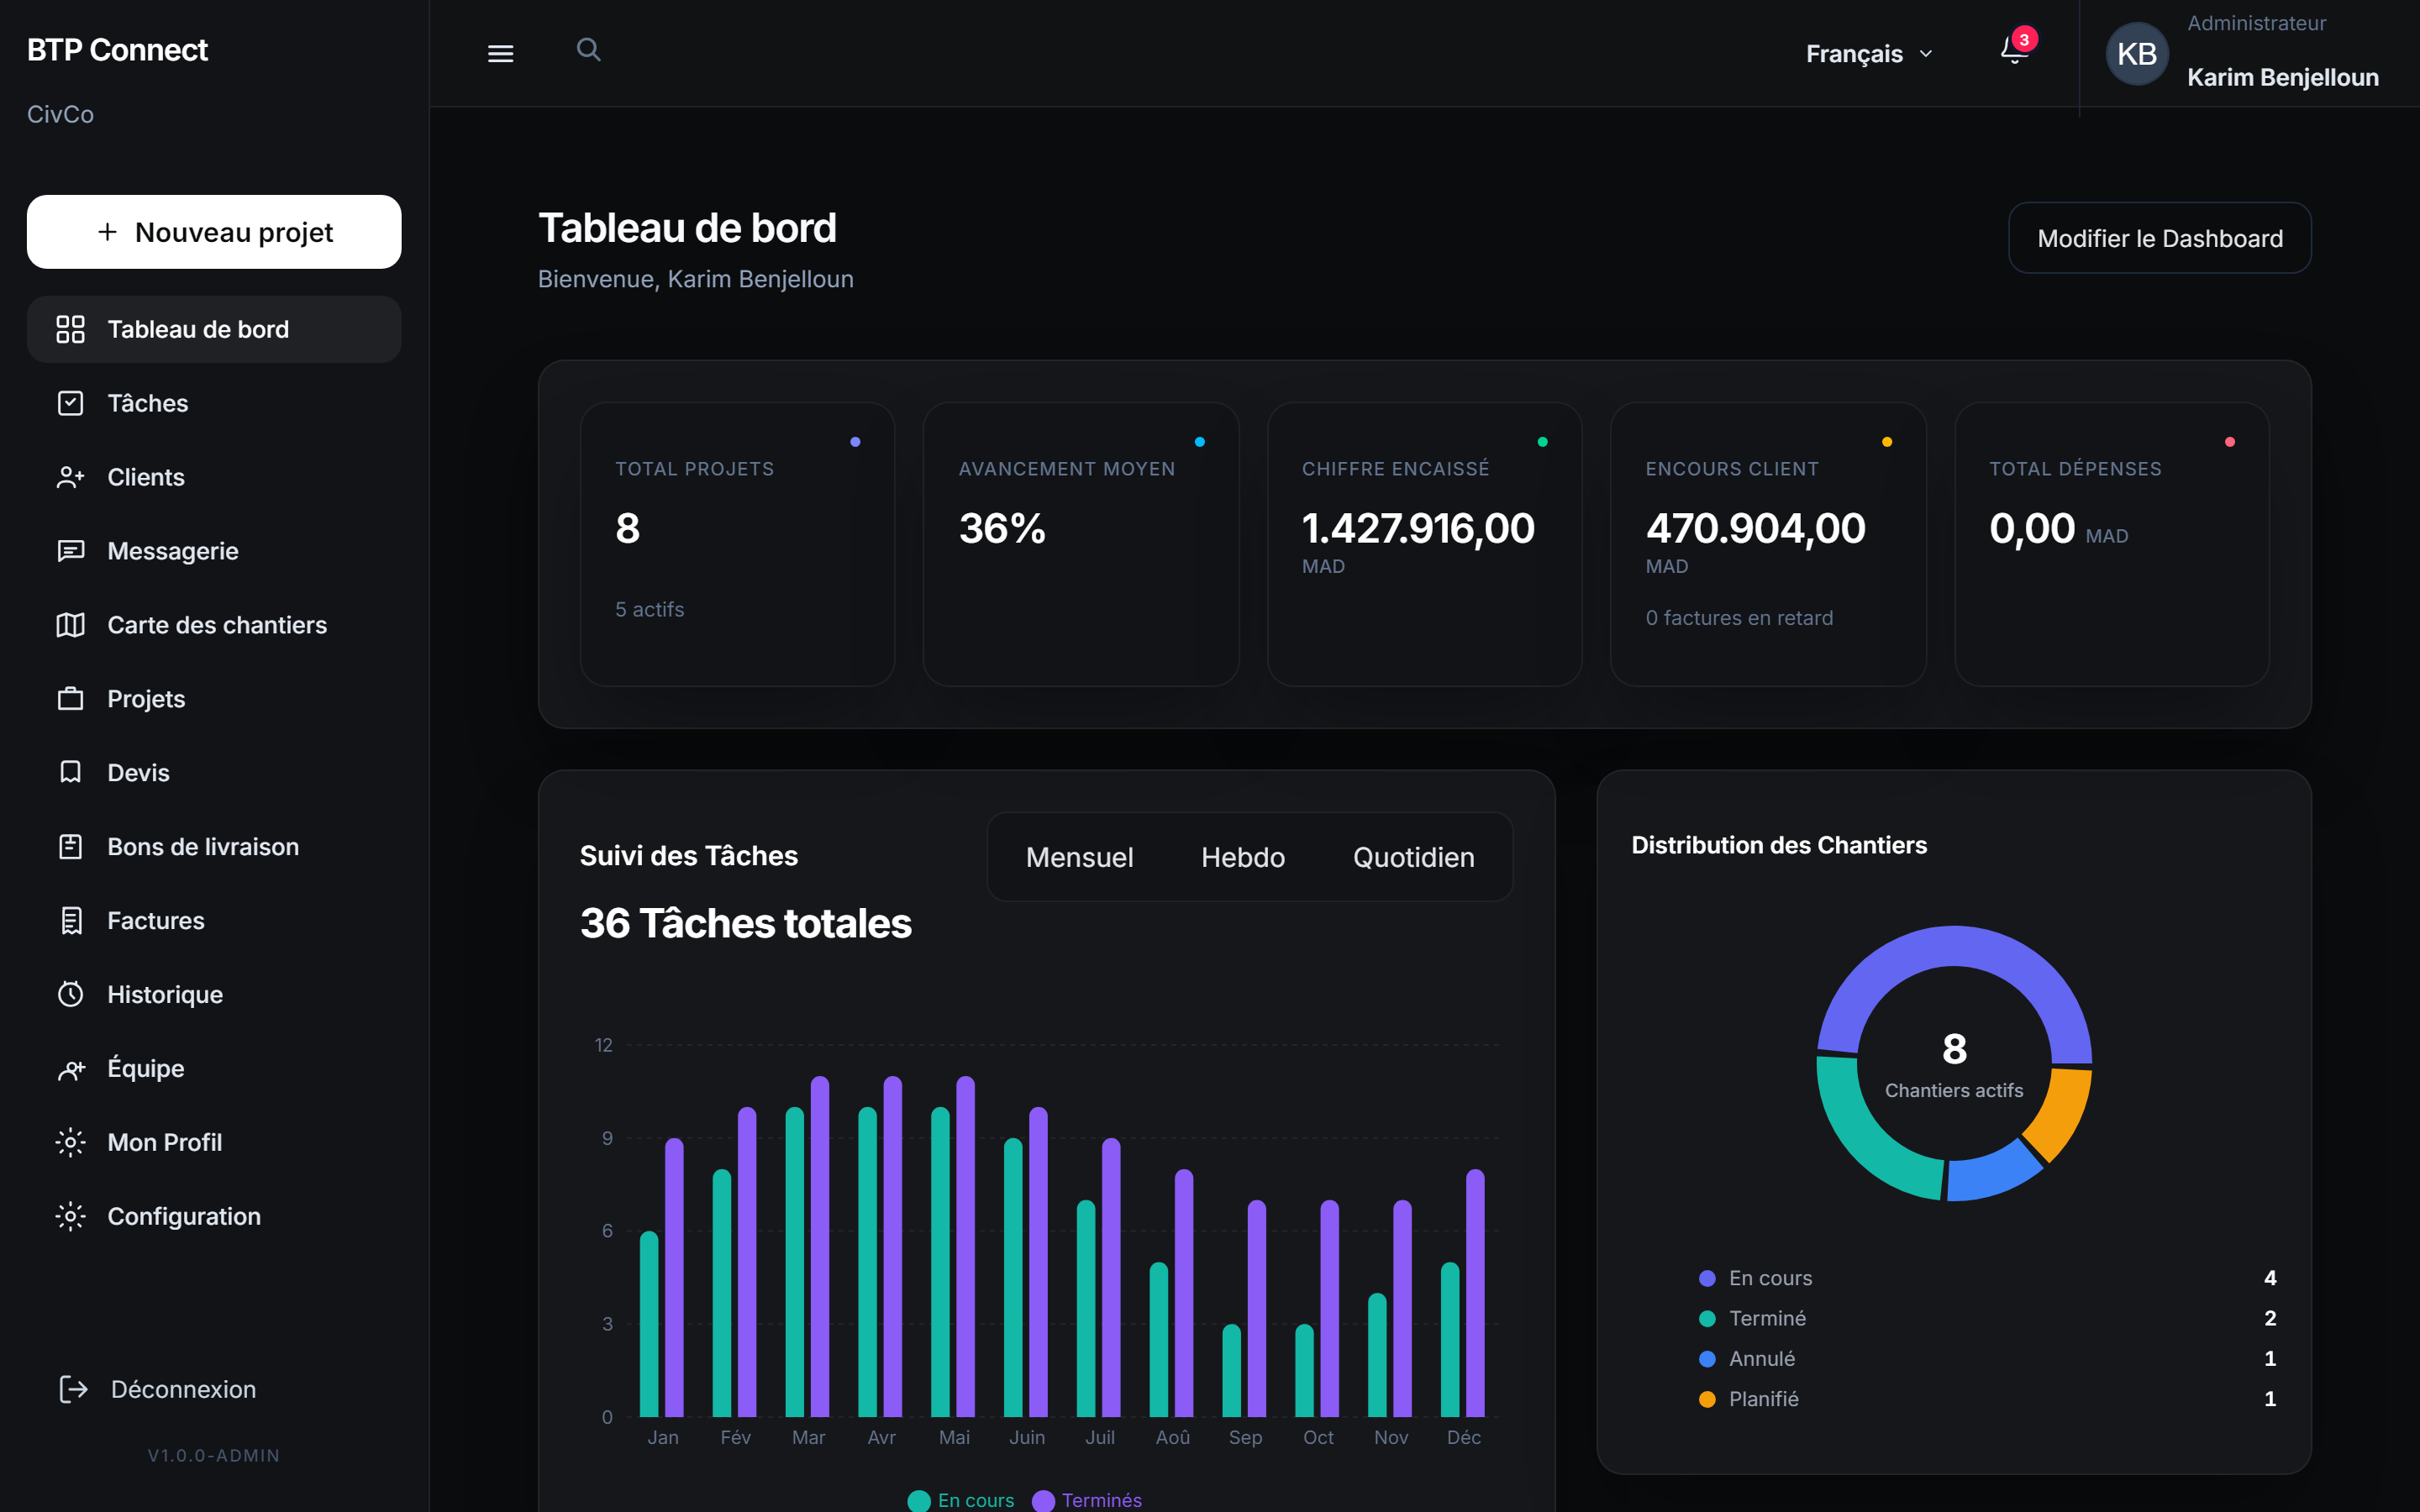
\includegraphics[width=\textwidth]{dashboard.png}
  \caption{Tableau de bord : vue synthétique de l'activité (projets, tâches, indicateurs)}
  \label{fig:dashboard}
\end{figure}

Le tableau de bord (Figure~\ref{fig:dashboard}) agrège les informations essentielles :
nombre de projets en cours, tâches prioritaires, graphiques d'avancement (Recharts)
et accès rapide aux modules. Les widgets affichés dépendent des permissions de
l'utilisateur connecté.

\medskip

Les widgets sont configurés dynamiquement : un administrateur voit l'ensemble des
indicateurs (projets actifs, factures en attente, tâches en retard), tandis qu'un
technicien ne voit que ses tâches assignées et les projets auxquels il participe.
Les graphiques Recharts illustrent l'évolution de l'avancement et la répartition
des projets par statut.

\subsection{Gestion des projets}

\begin{figure}[H]
  \centering
  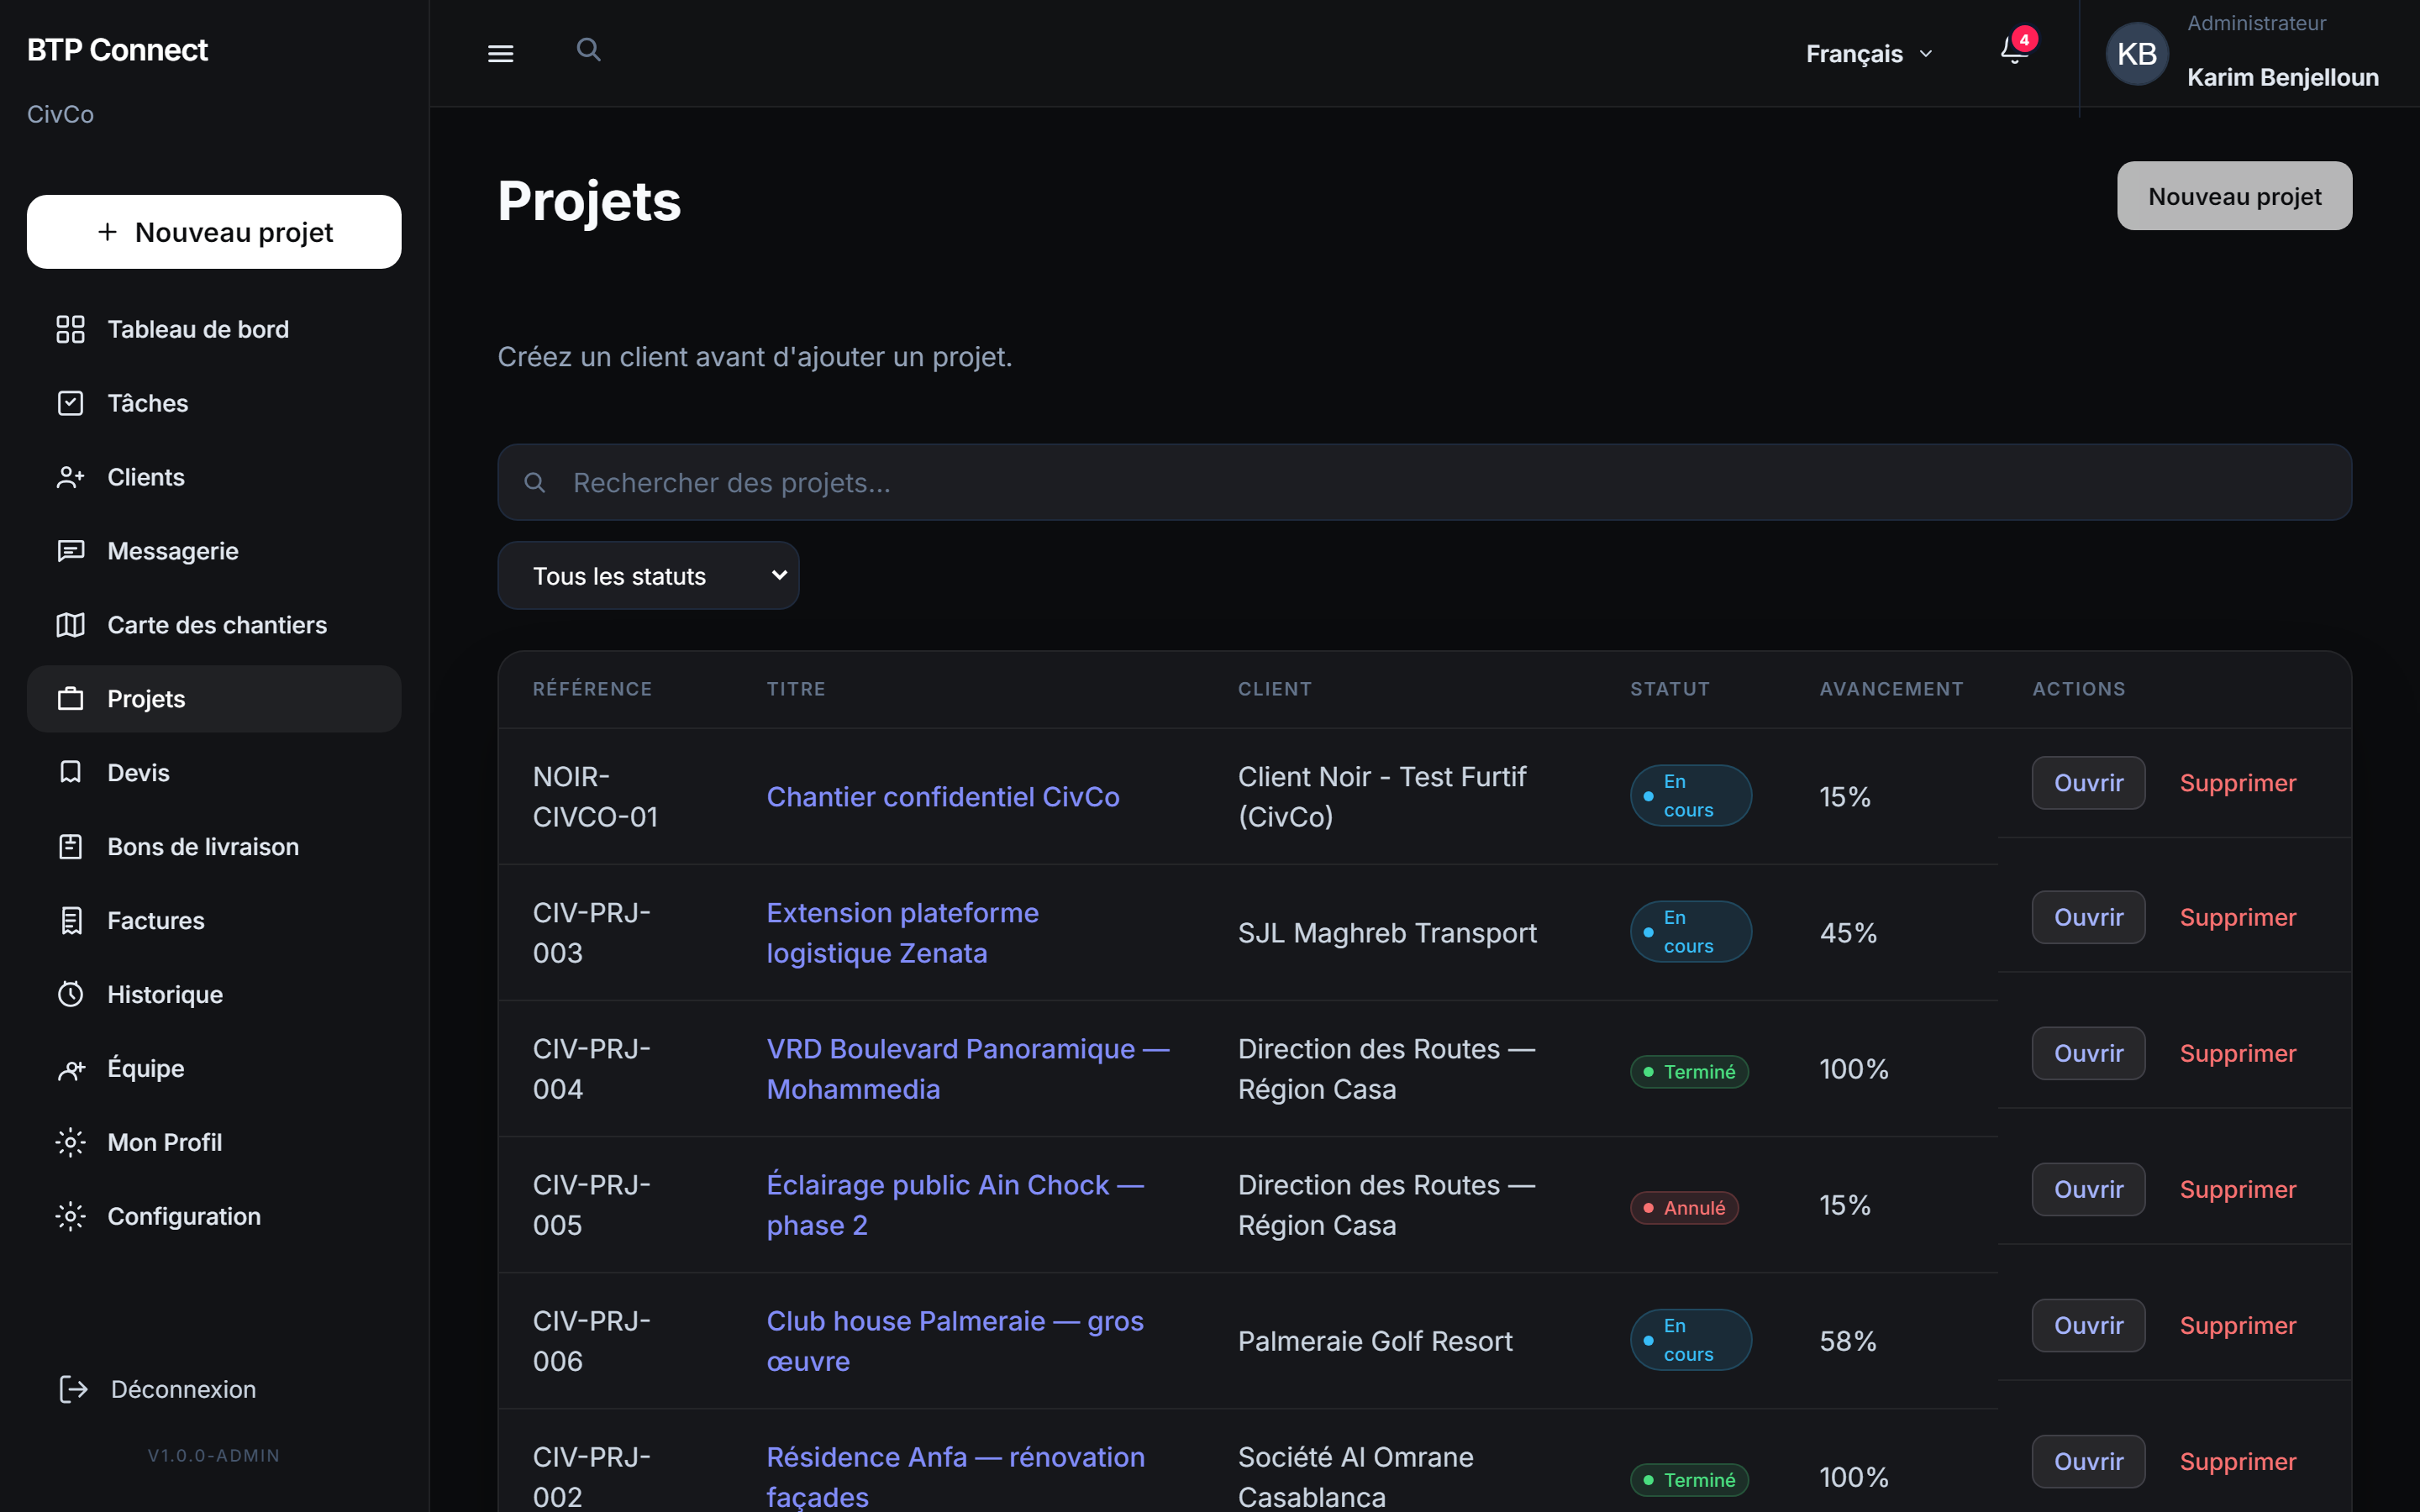
\includegraphics[width=\textwidth]{projects.png}
  \caption{Module Projets : liste des chantiers et fiche détail (phases, équipe, documents)}
  \label{fig:projects}
\end{figure}

Le module Projets (Figure~\ref{fig:projects}) permet de créer, consulter et modifier
les chantiers. La fiche détail est organisée en onglets : informations générales,
phases, tâches, équipe, devis/factures liés, contrats, dépenses et médias.

\medskip

La liste des projets propose des filtres par statut, client et nature de chantier.
La fiche détail centralise toutes les informations d'un chantier : depuis un seul
écran, le chef de projet peut consulter l'avancement des phases, réaffecter un
collaborateur, joindre un document ou créer un devis lié au projet.

\subsection{Gestion des clients}

\begin{figure}[H]
  \centering
  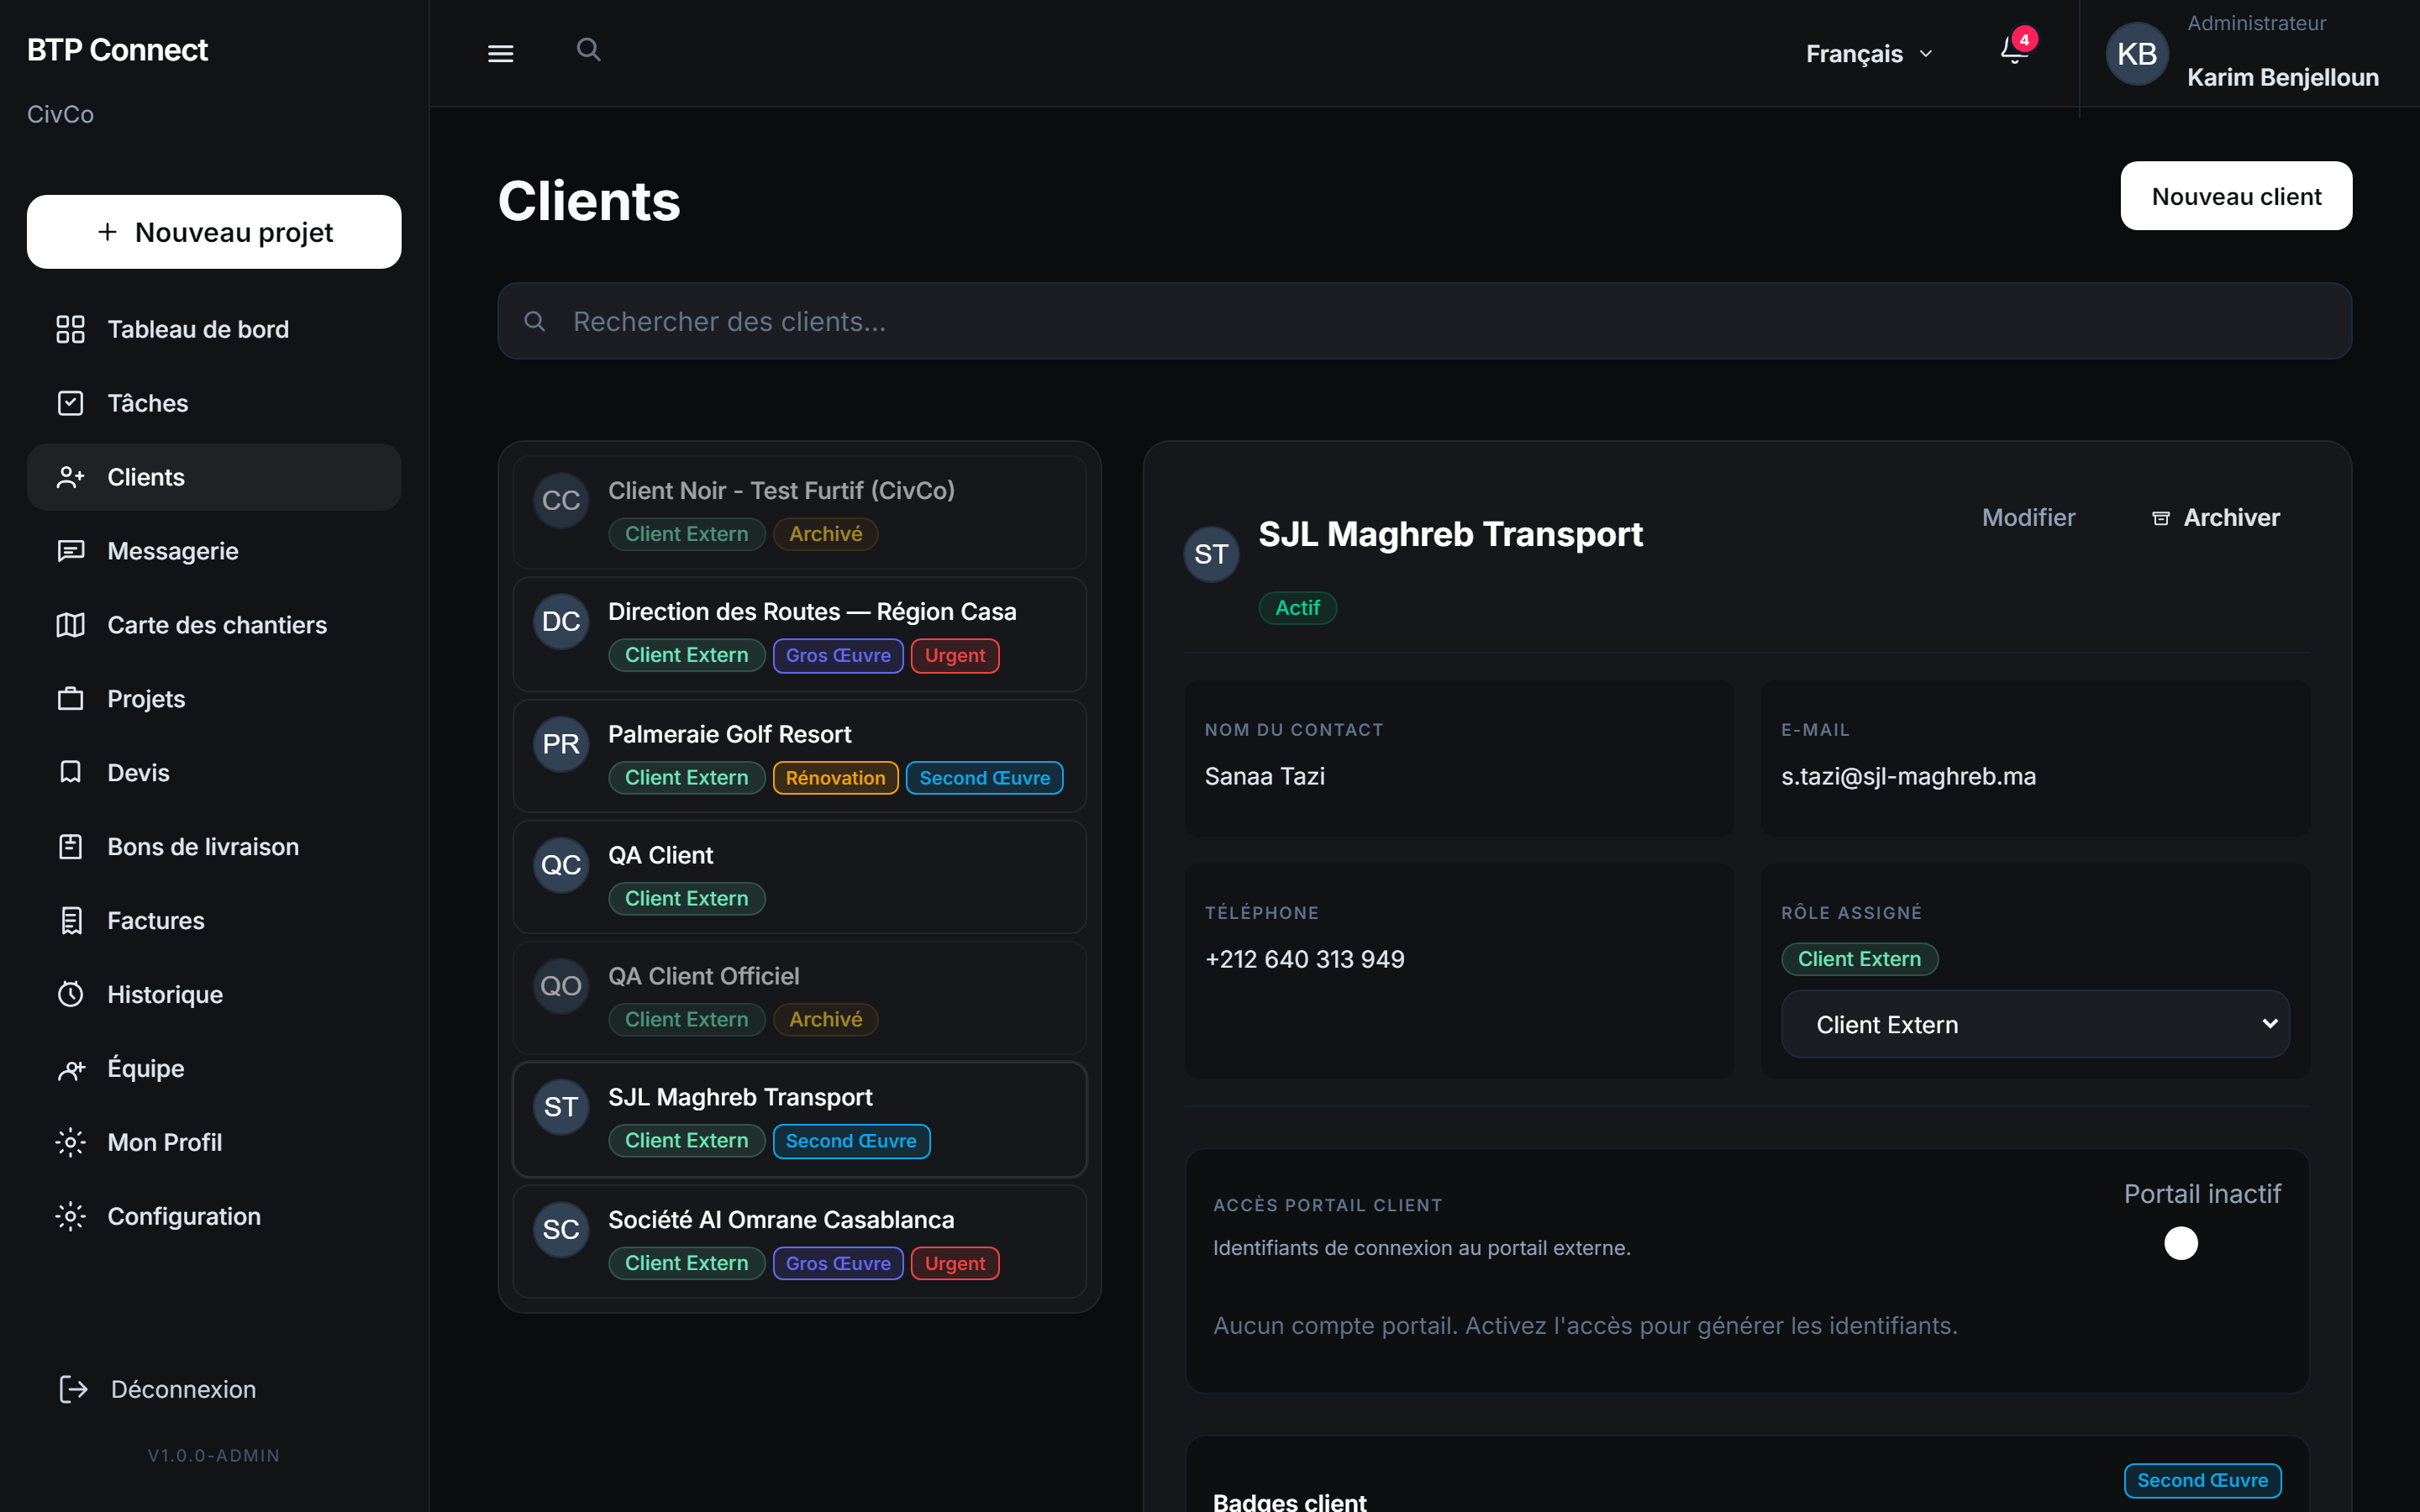
\includegraphics[width=\textwidth]{clients.png}
  \caption{Module Clients : fiches clients, contacts et archivage}
  \label{fig:clients}
\end{figure}

Le module Clients (Figure~\ref{fig:clients}) centralise les maîtres d'ouvrage et
clients commerciaux. L'administrateur peut provisionner un accès portail pour un
client externe directement depuis la fiche client.

\medskip

Chaque fiche client regroupe les coordonnées, les contacts associés, les badges
métier (Gros Œuvre, Urgent, etc.), l'historique des projets et l'état du compte
portail. L'archivage est sécurisé par une modale de confirmation pour éviter les
suppressions accidentelles.

\subsection{Documents commerciaux}

\begin{figure}[H]
  \centering
  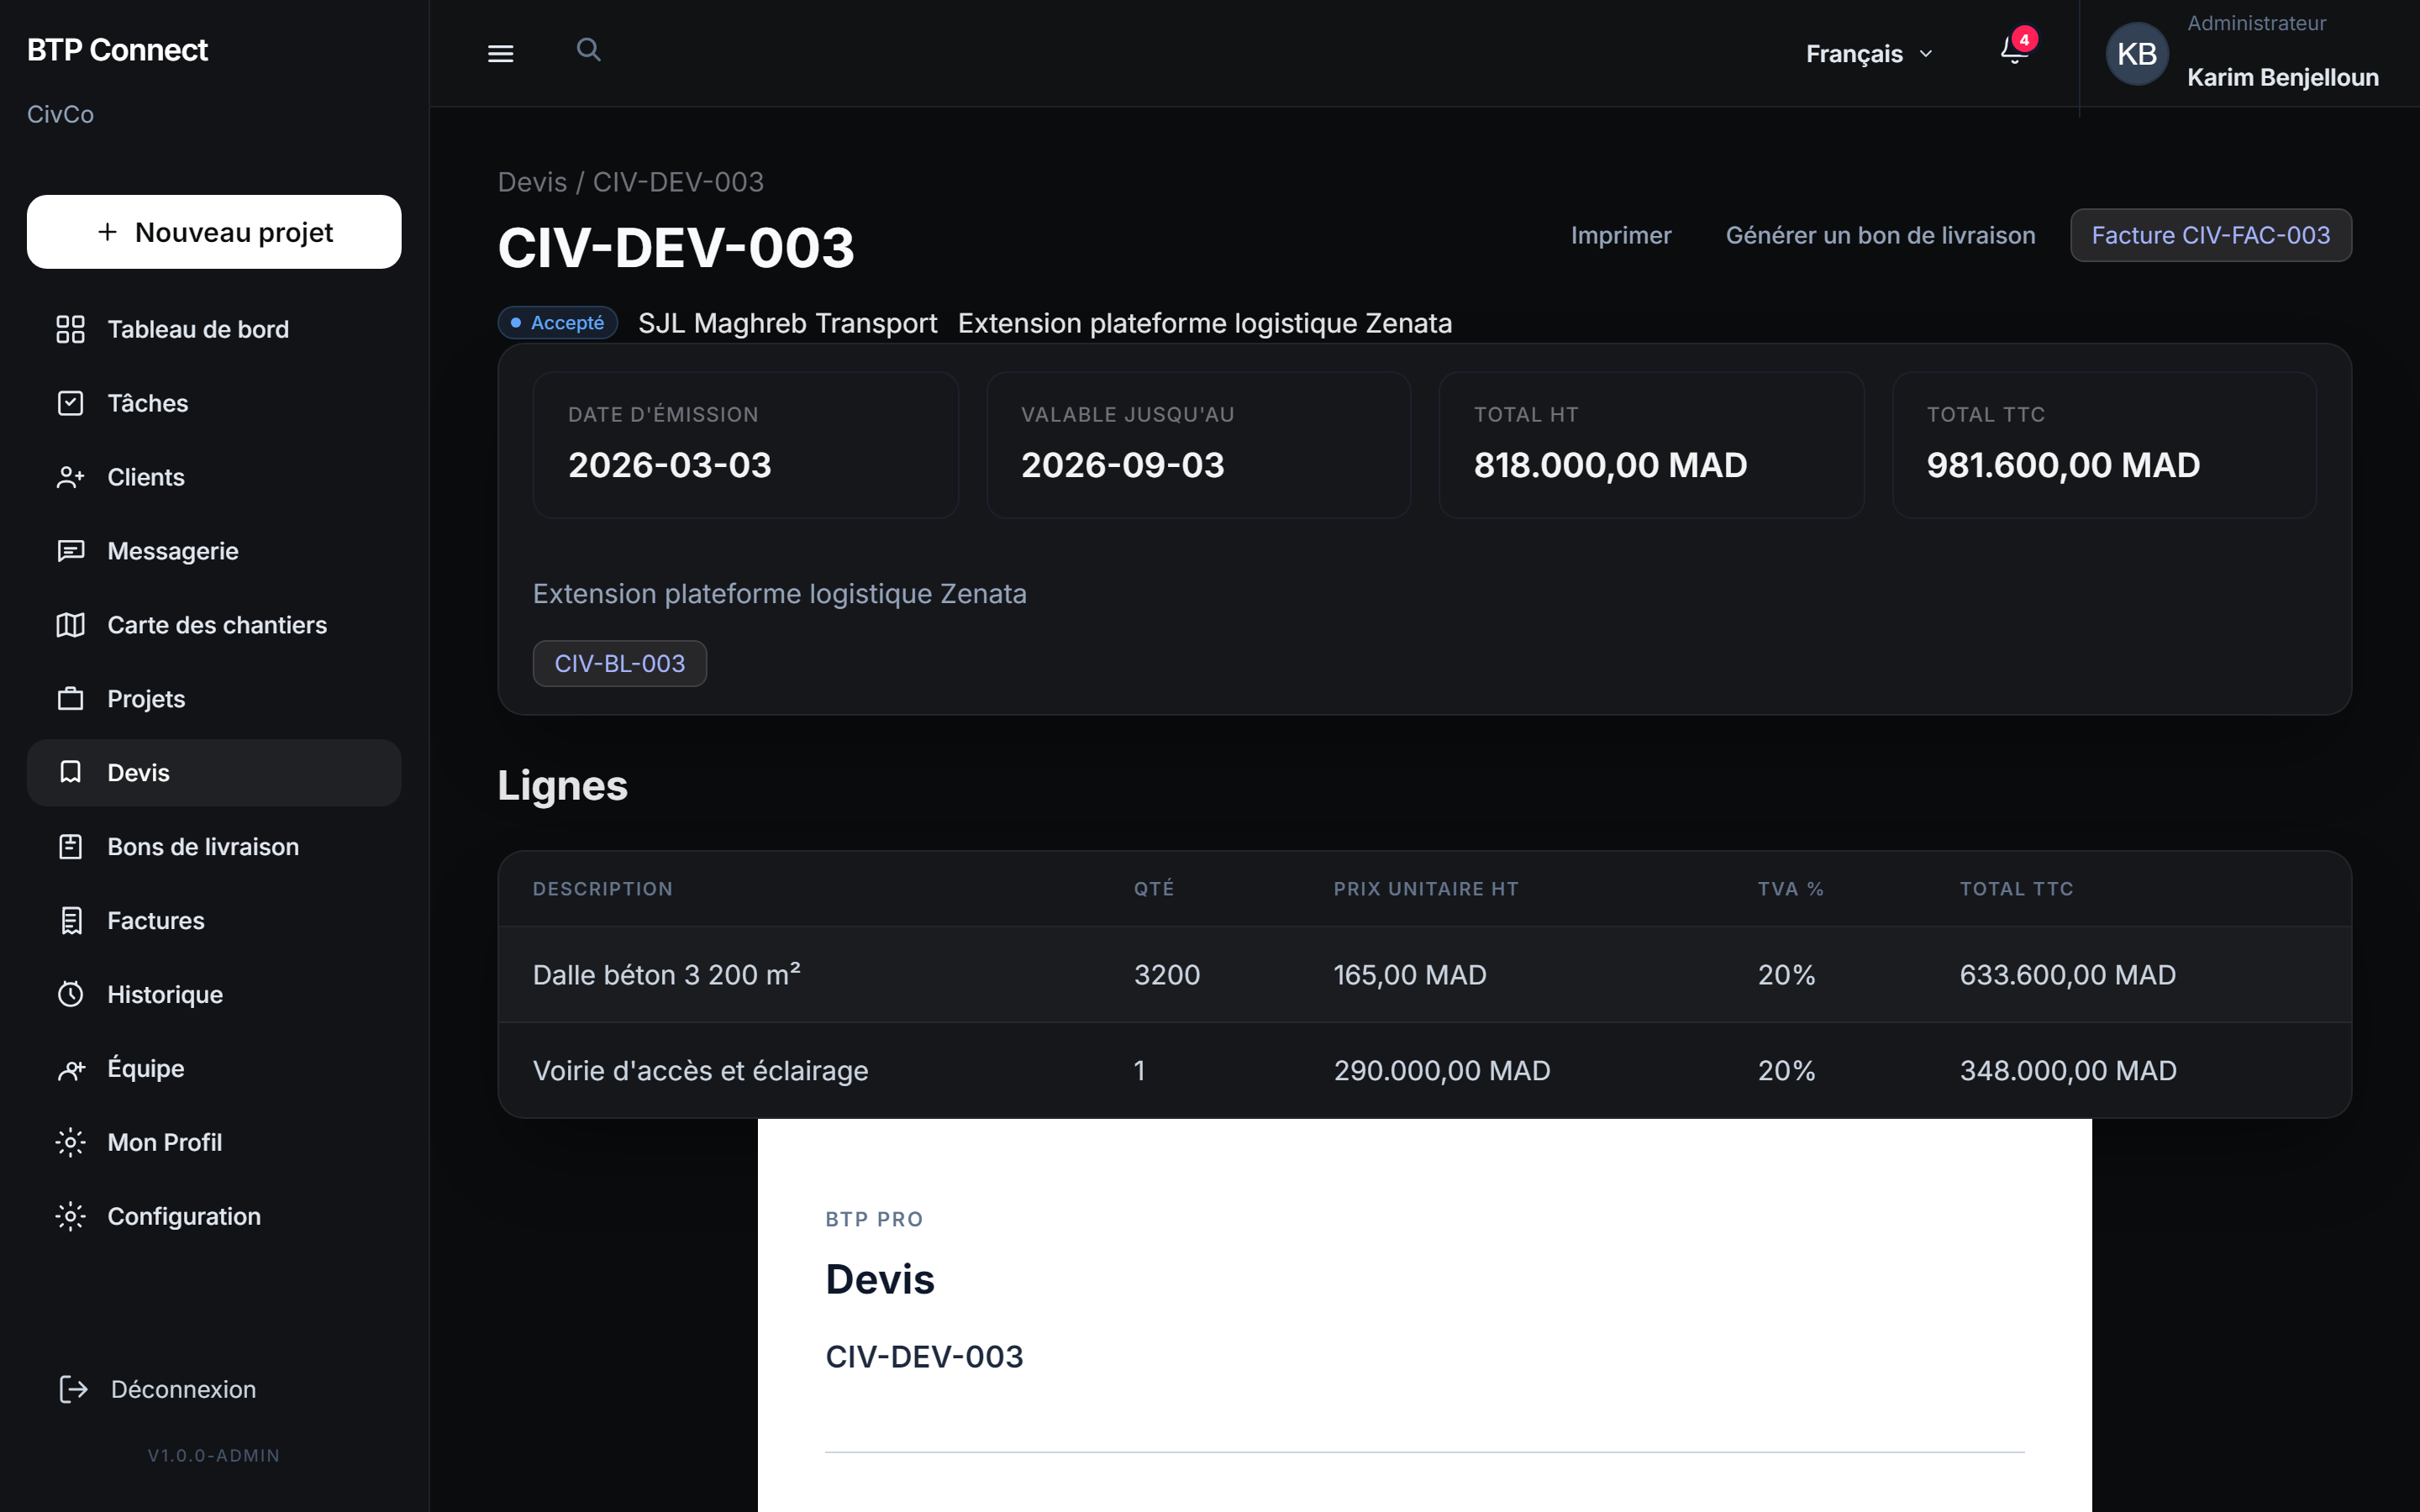
\includegraphics[width=\textwidth]{quotes.png}
  \caption{Module Devis : création avec lignes de détail et calcul automatique des totaux}
  \label{fig:quotes}
\end{figure}

\begin{figure}[H]
  \centering
  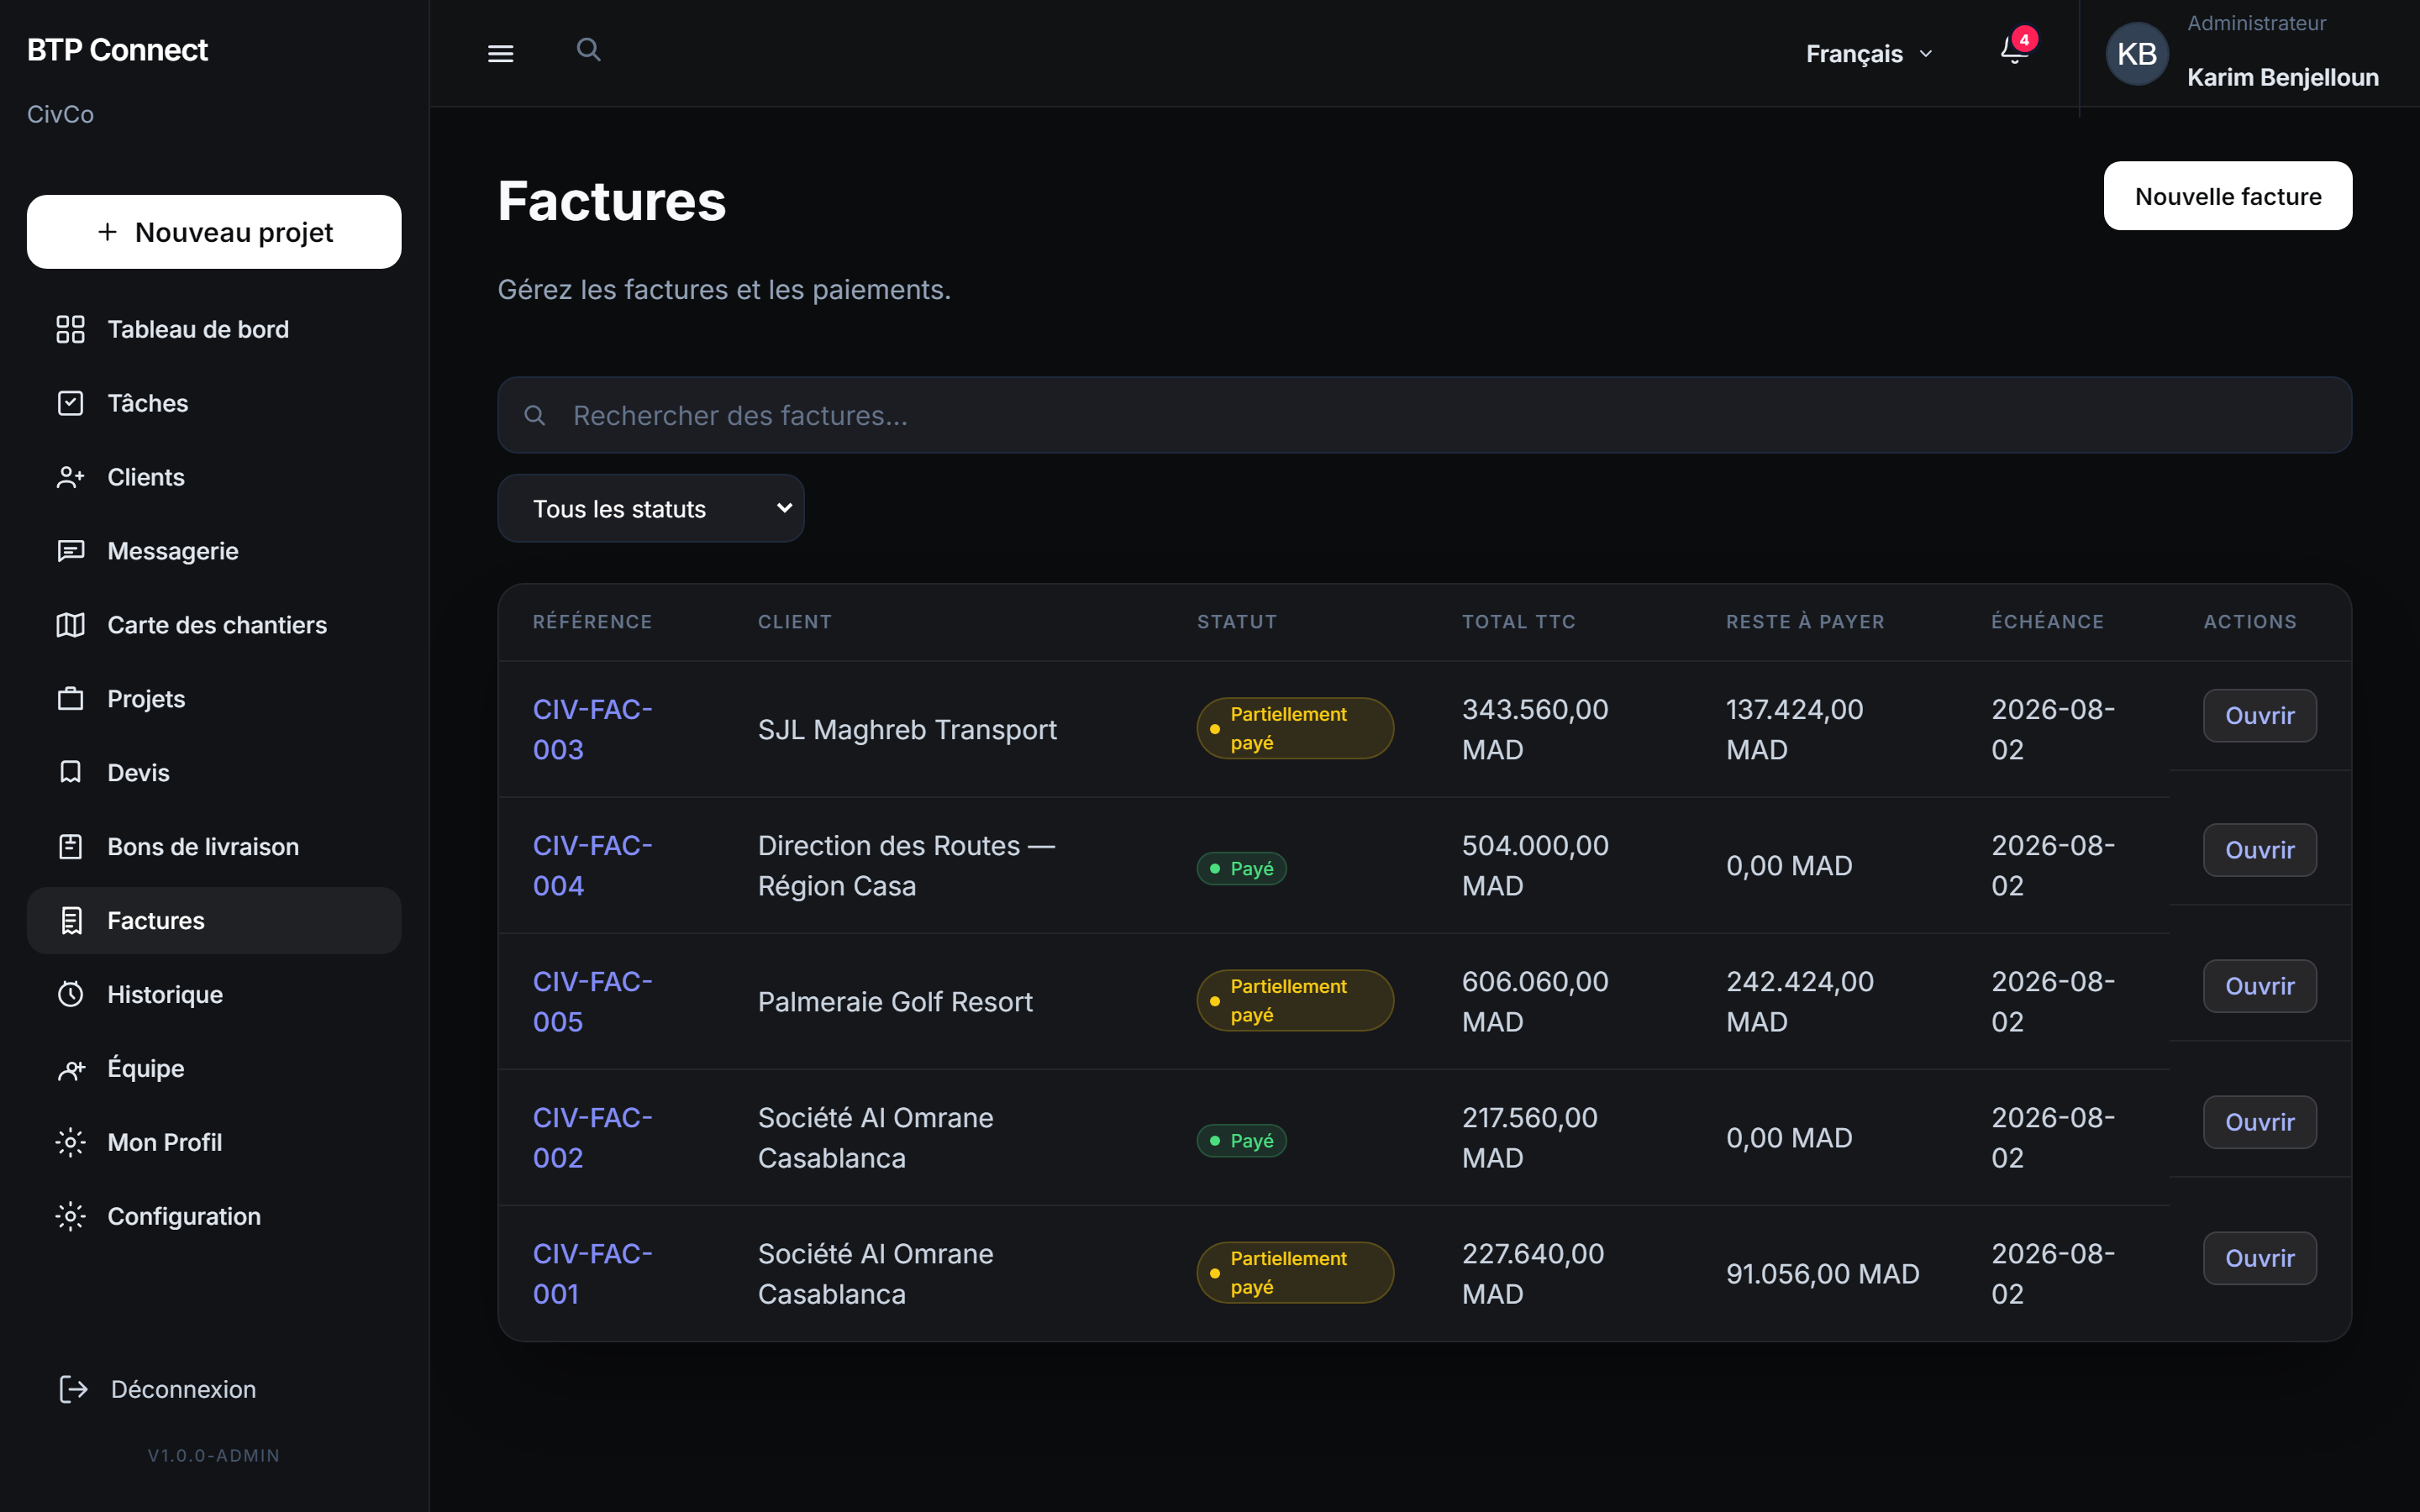
\includegraphics[width=\textwidth]{invoices.png}
  \caption{Module Factures : suivi des factures et état de paiement}
  \label{fig:invoices}
\end{figure}

Les modules Devis et Factures (Figures~\ref{fig:quotes} et~\ref{fig:invoices})
permettent la production des documents commerciaux, leur impression (avec suivi
des copies officielles) et la conversion devis $\rightarrow$ facture en un clic.

\medskip

Le formulaire de création de devis permet d'ajouter dynamiquement des lignes de
prestation (description, quantité, prix unitaire HT, taux de TVA). Les totaux sont
recalculés en temps réel. L'impression s'effectue via un composant React dédié
(\texttt{CommercialPrintSheet}) qui génère une version formatée prête à l'envoi au
client, avec suivi du quota d'impressions officielles.

\subsection{Planification des tâches}

\begin{figure}[H]
  \centering
  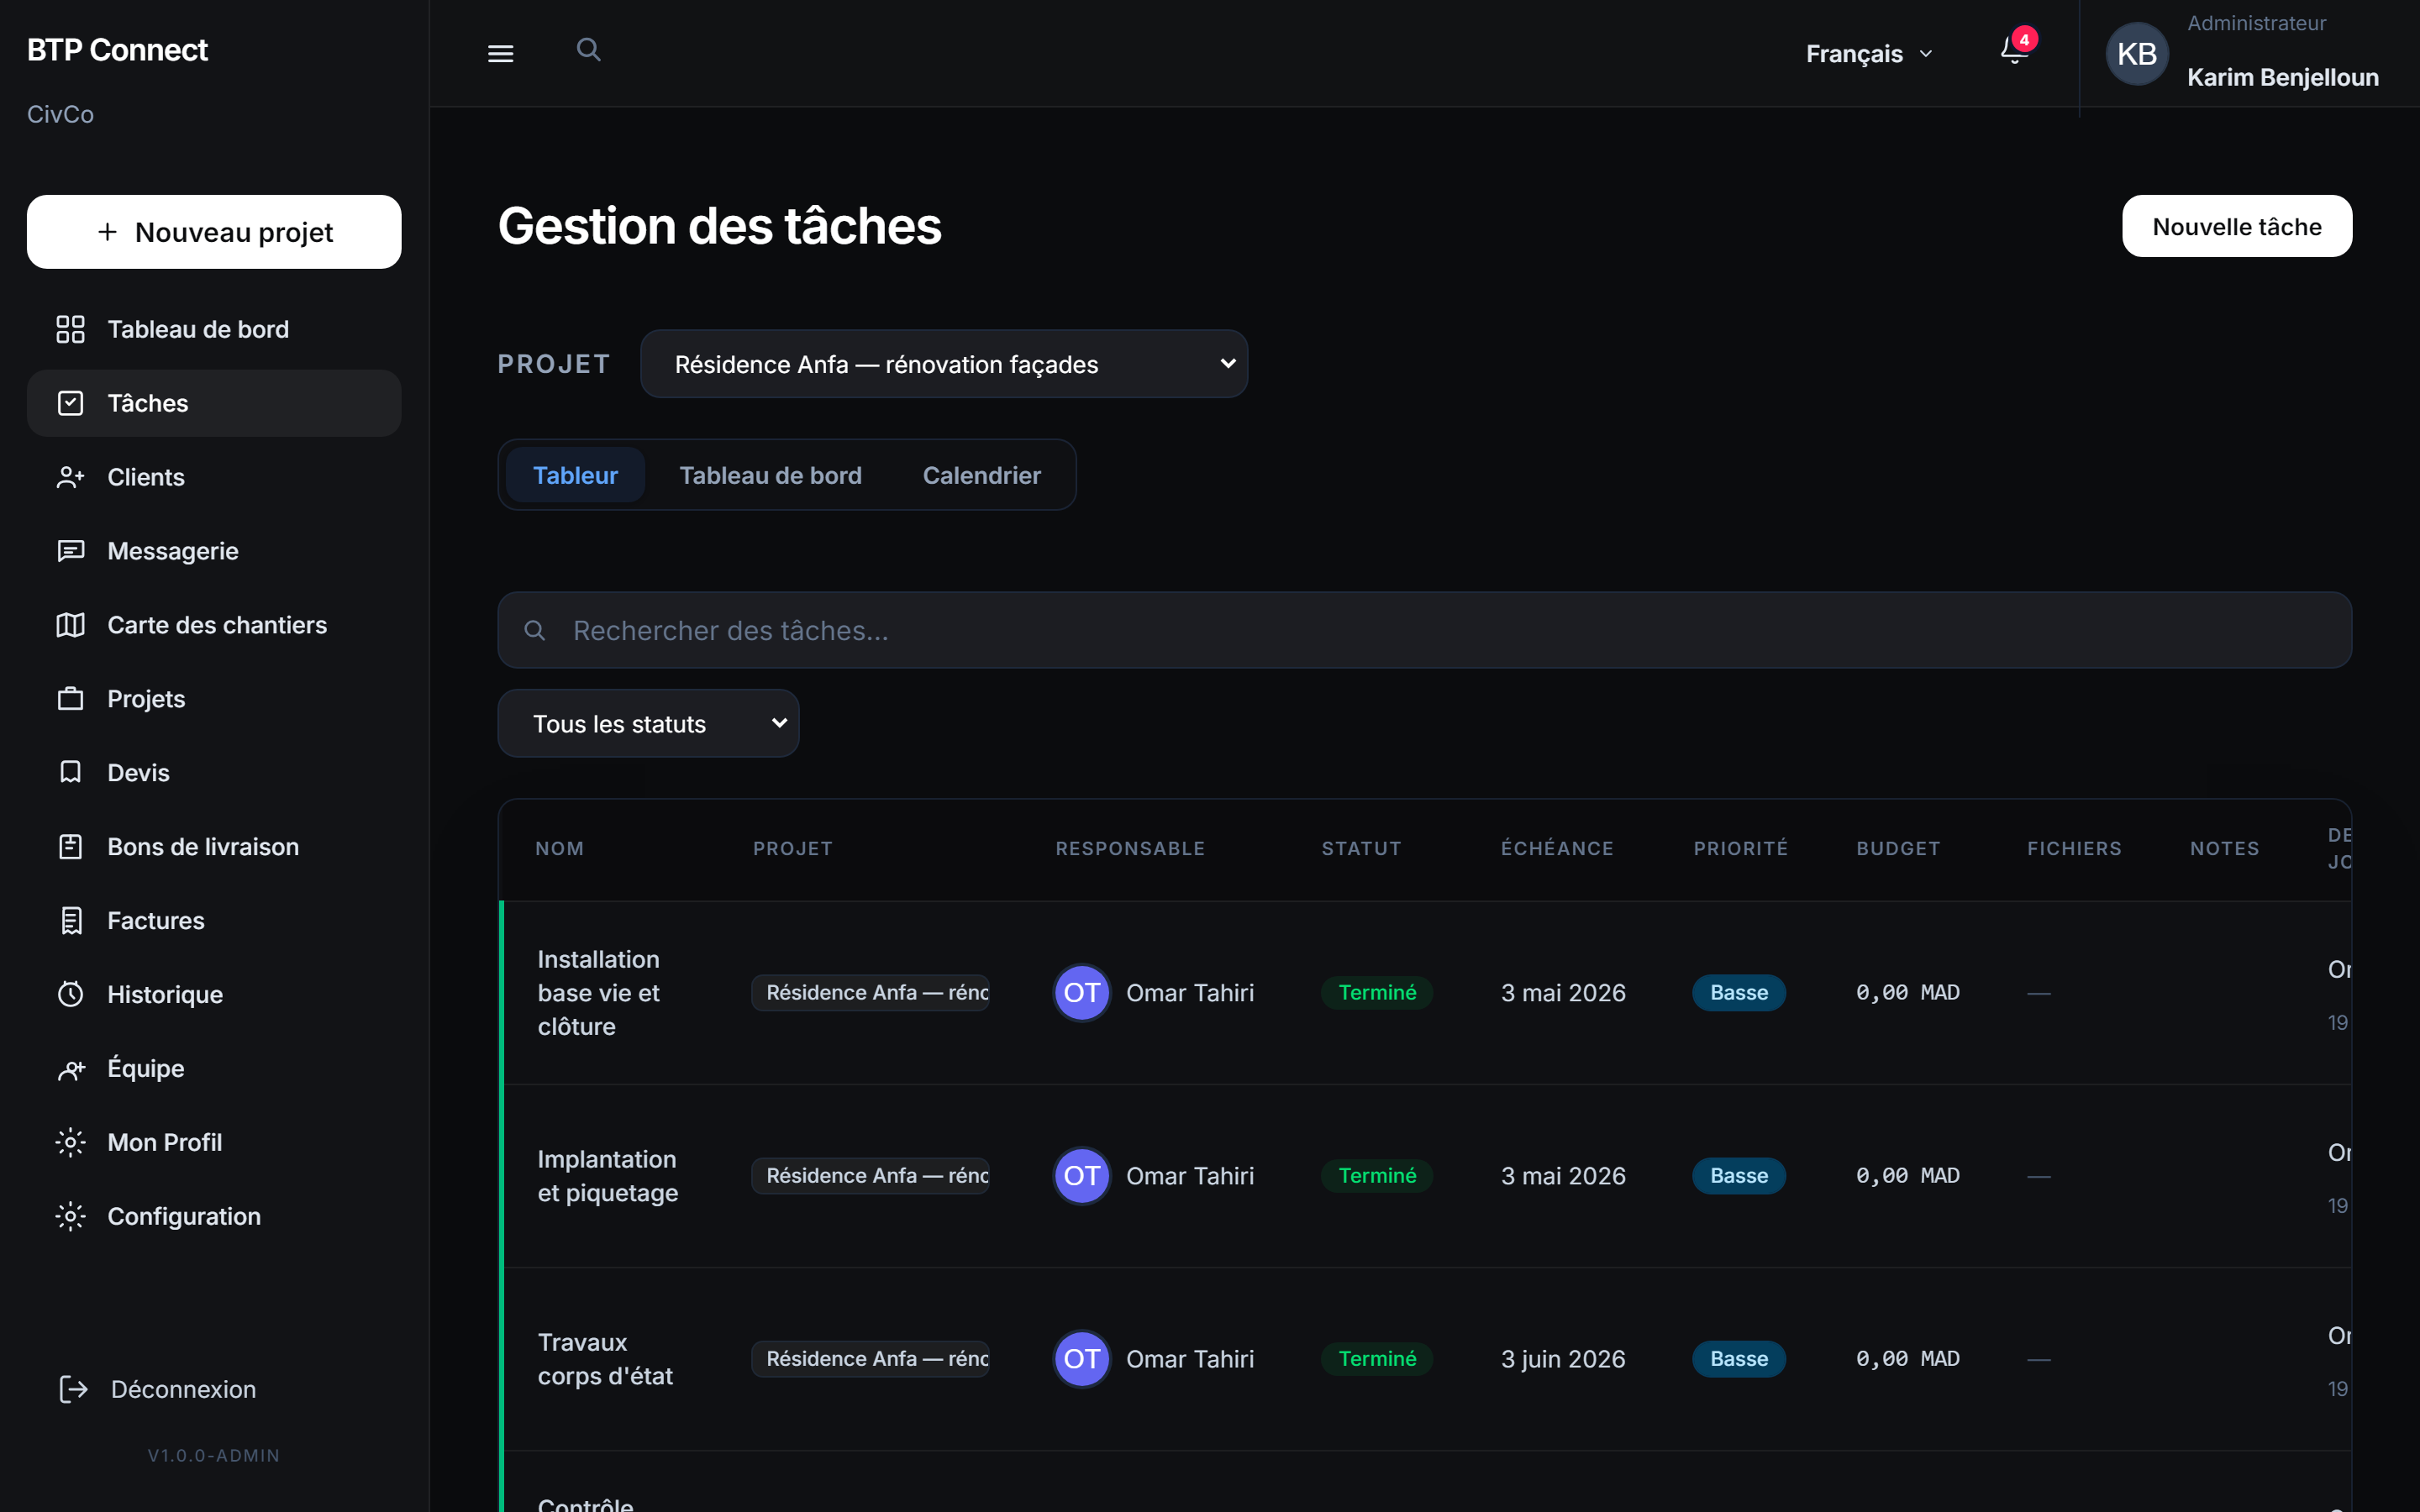
\includegraphics[width=\textwidth]{tasks.png}
  \caption{Module Tâches : planification, assignation et suivi par projet}
  \label{fig:tasks}
\end{figure}

Le module Tâches (Figure~\ref{fig:tasks}) offre une vue tableau des missions
opérationnelles, filtrable par statut, projet et assigné. Les chefs de projet
peuvent créer et assigner des tâches ; les utilisateurs internes consultent
leurs tâches propres.

\medskip

Le module propose une vue tableau avec tri par date d'échéance, filtre par statut
(à faire, en cours, terminé) et code couleur pour les tâches en retard. La création
d'une tâche associe obligatoirement un projet, une phase et un responsable, garantissant
la traçabilité de l'assignation.

\subsection{Carte des chantiers}

\begin{figure}[H]
  \centering
  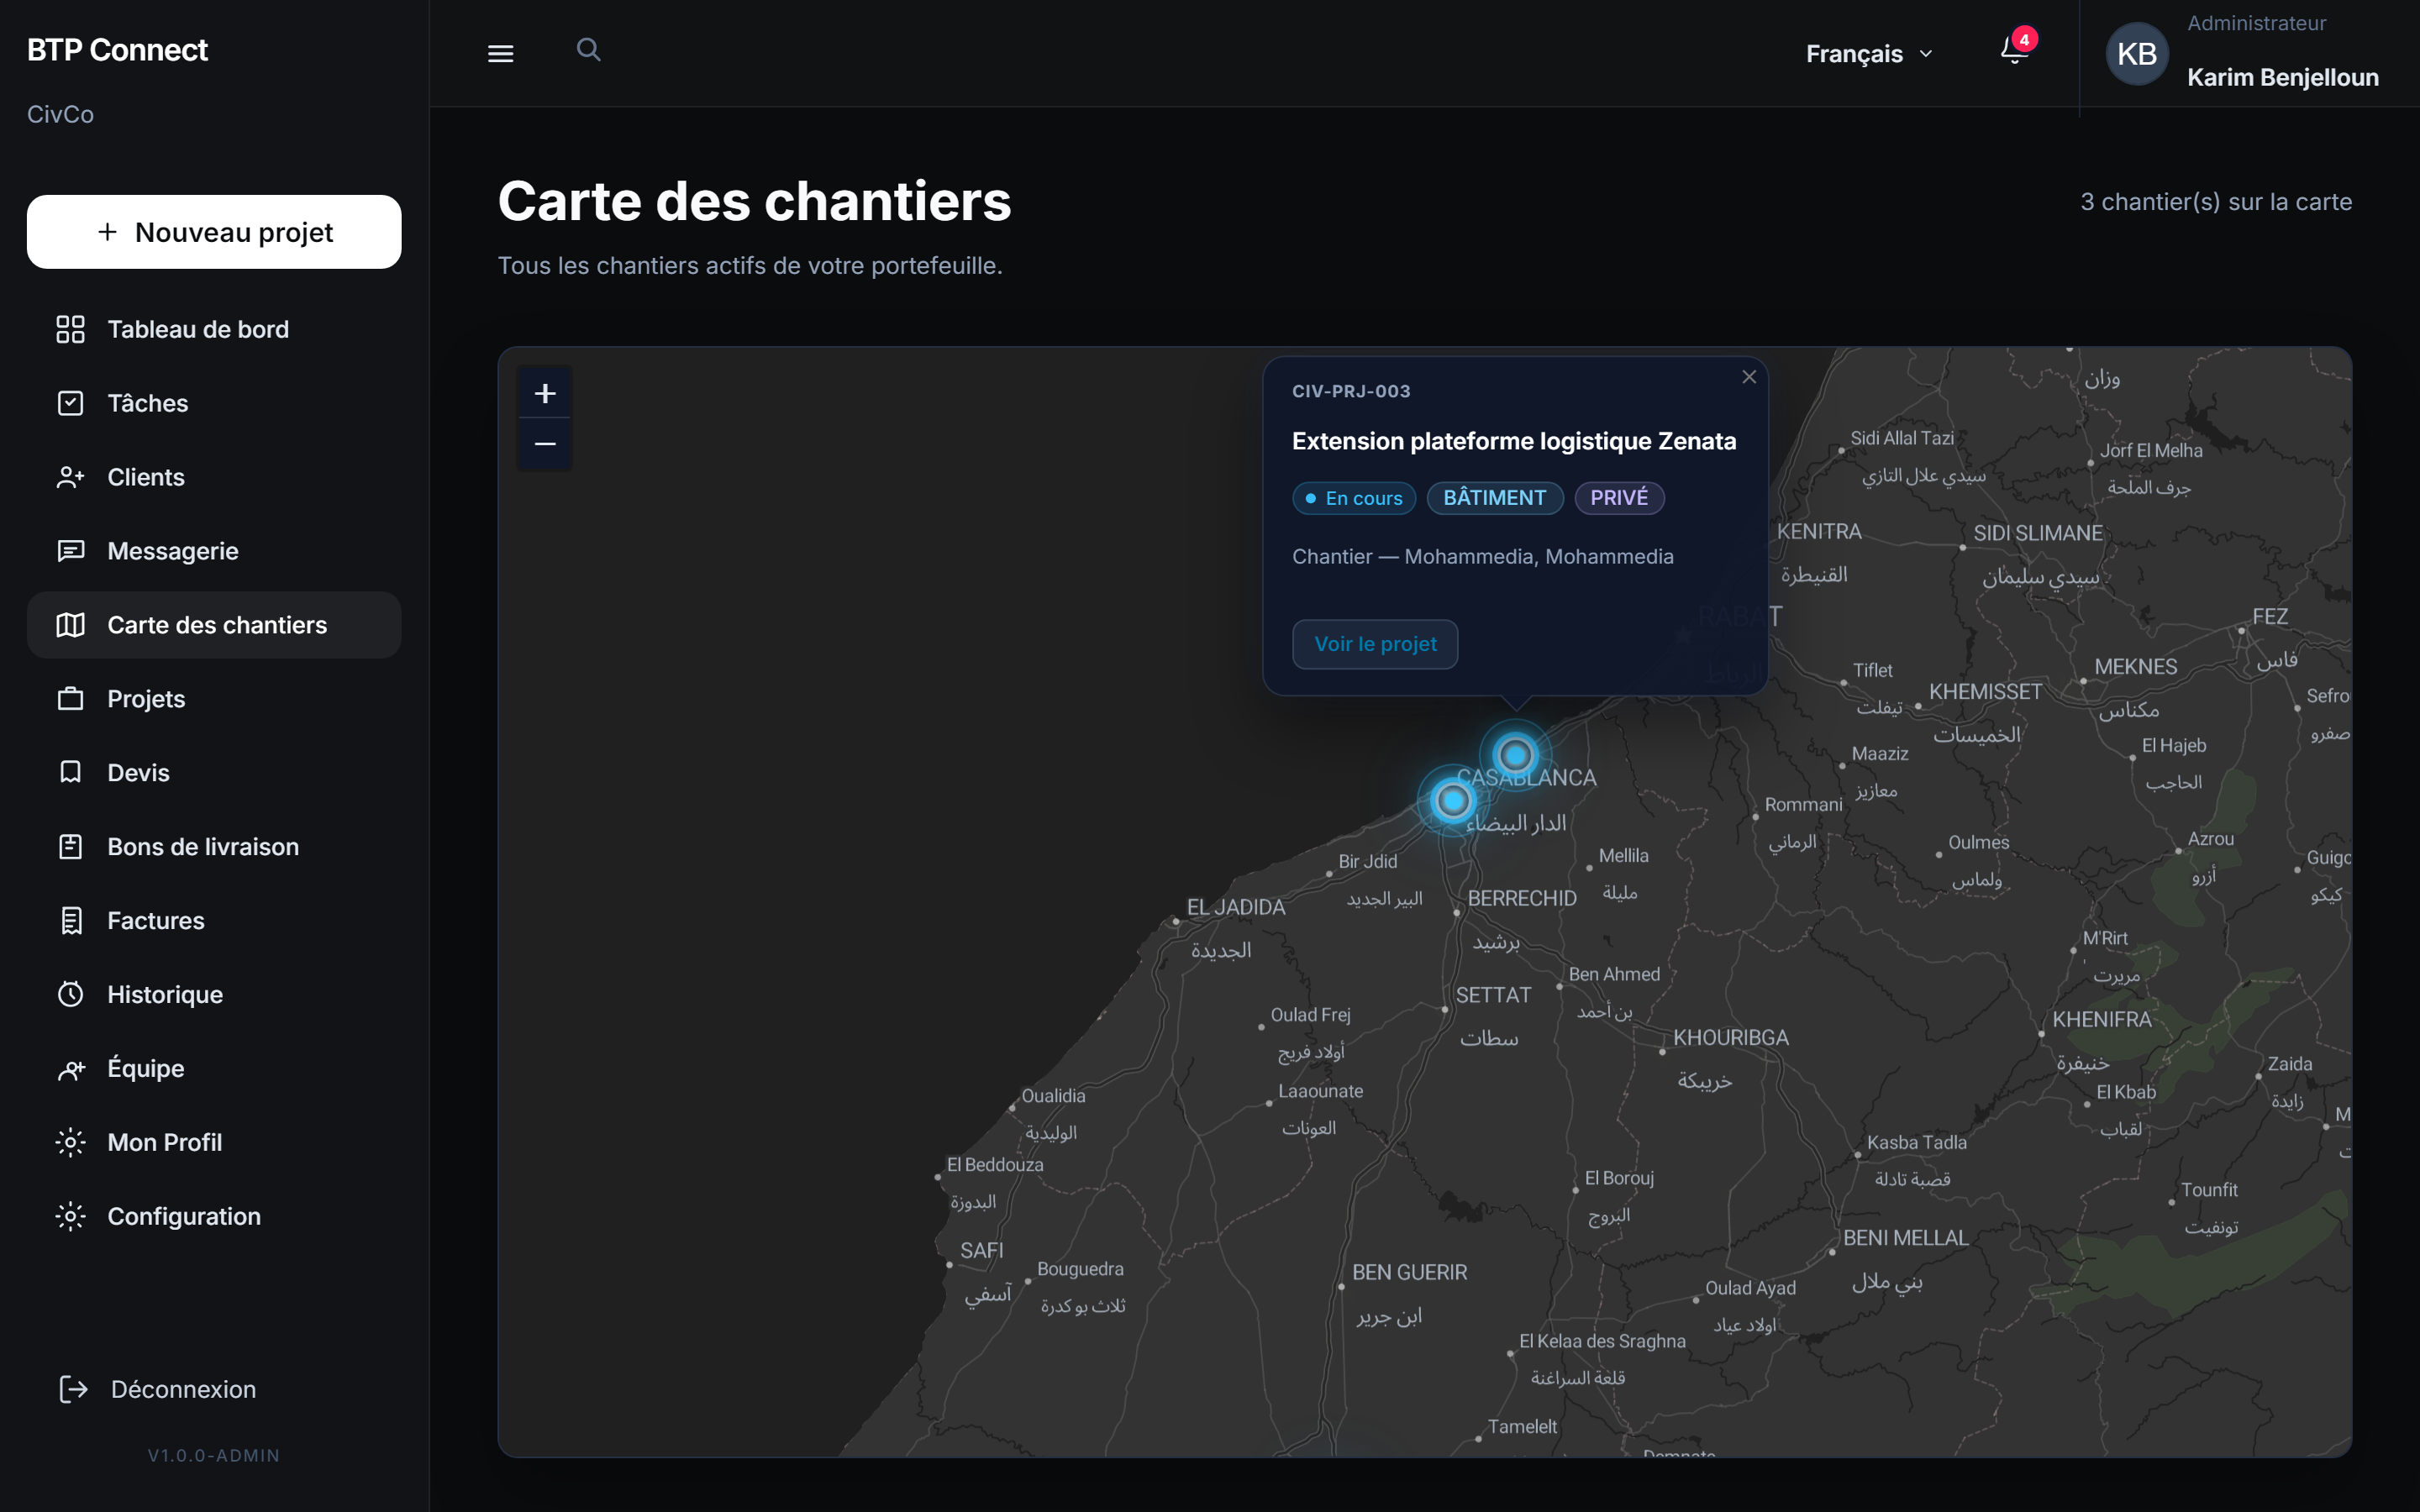
\includegraphics[width=\textwidth]{map.png}
  \caption{Carte des projets : visualisation géographique des chantiers (Leaflet)}
  \label{fig:map}
\end{figure}

La carte (Figure~\ref{fig:map}) affiche les projets géolocalisés sur une carte
interactive Leaflet, utile pour visualiser la répartition géographique des
chantiers de CIVCO BTP.

\medskip

Chaque marqueur sur la carte correspond à un projet géolocalisé. Un clic affiche un
résumé (référence, client, statut, avancement) et un lien vers la fiche détail.
Cette visualisation est particulièrement utile pour la direction et les chefs de
projet qui gèrent plusieurs chantiers répartis sur différentes zones géographiques
du Grand Casablanca et au-delà.

\subsection{Portail client}

\begin{figure}[H]
  \centering
  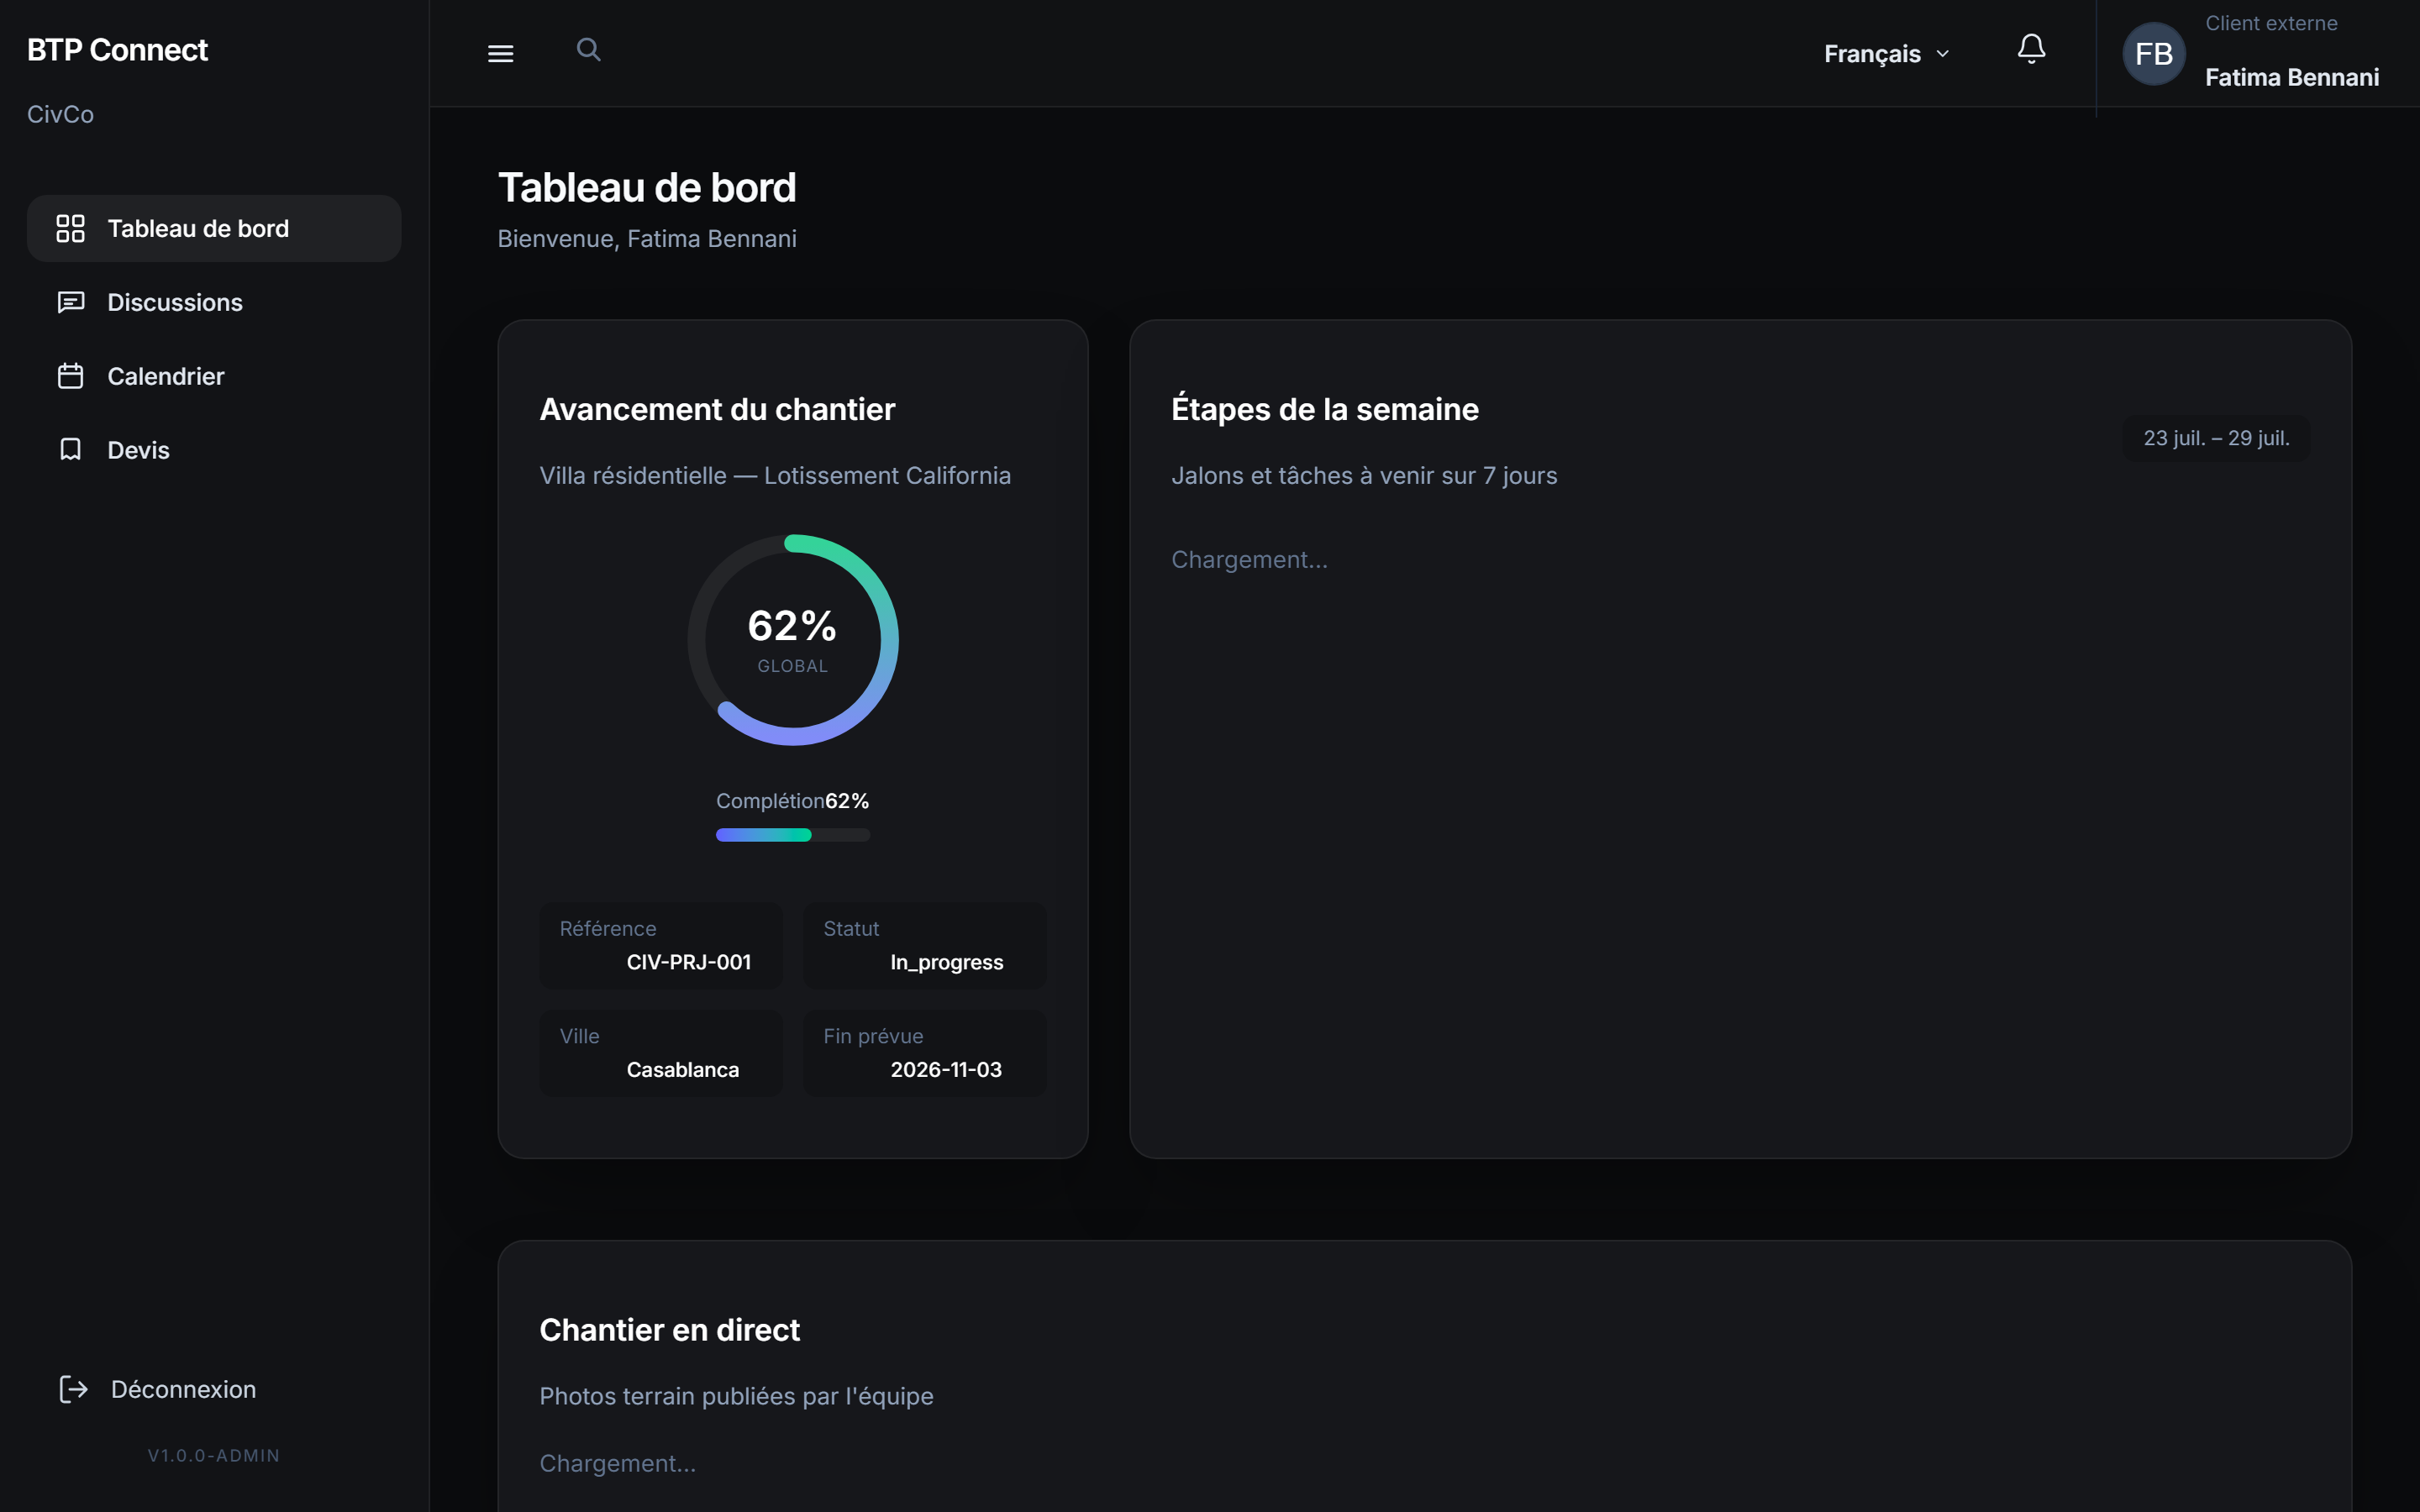
\includegraphics[width=\textwidth]{portal.png}
  \caption{Portail client : consultation des projets, acceptation de devis et signature}
  \label{fig:portal}
\end{figure}

Le portail client (Figure~\ref{fig:portal}) offre une interface simplifiée aux
clients externes : consultation de l'avancement, acceptation de devis, signature
de contrats et messagerie avec l'équipe projet.

\medskip

L'interface portail est volontairement distincte de l'ERP interne : navigation
réduite à quatre entrées (tableau de bord, discussions, calendrier, devis), sans
accès aux modules de gestion internes (projets, facturation, configuration).
Les routes React sont regroupées sous le préfixe \texttt{/portal/*} et protégées
par le middleware d'authentification ; un utilisateur possédant le rôle
\texttt{client\_extern} est automatiquement redirigé vers le portail après
connexion, tandis qu'un collaborateur interne ne peut pas y accéder.

\medskip

\textbf{Tableau de bord client.} L'écran principal (Figure~\ref{fig:portal})
présente trois blocs d'information. Le widget \textit{Avancement du chantier}
affiche un indicateur circulaire (\texttt{ProgressRing}) alimenté par le champ
\texttt{progress\_percent} du projet, accompagné de la référence chantier, du
statut, de la ville et de la date de fin prévue. Le panneau \textit{Étapes de
la semaine} liste les jalons et tâches à échéance sur les sept prochains jours,
filtrés par projet sélectionné. Enfin, le fil \textit{Chantier en direct}
(\texttt{ChantierLiveFeed}) expose les photos terrain publiées par l'équipe
CIVCO BTP, rafraîchies périodiquement pour offrir une visibilité continue
sur l'avancement des travaux.

\medskip

\textbf{Parcours documentaire et contractuel.} Depuis l'onglet \textit{Devis},
le client consulte les propositions commerciales qui le concernent et peut
accepter un devis en un clic ; le statut est immédiatement mis à jour côté
serveur. Pour les contrats, le composant \texttt{ClientContractSignature}
intègre un pad de signature tactile (canvas HTML5) : la signature est capturée,
transmise à l'API et associée au document contractuel, déclenchant la mise à
jour du statut et la notification de l'équipe projet.

\medskip

\textbf{Provisionnement et sécurité.} L'accès portail est créé par
l'administrateur depuis la fiche client (module Clients, Chapitre~4) : un
identifiant de connexion est généré, associé au client concerné via le champ
\texttt{client\_id} de l'utilisateur, et activé ou désactivé à la demande.
Toutes les requêtes API du portail sont filtrées par ce lien client $\rightarrow$
projet : un client externe ne voit que ses propres chantiers, devis et
échanges, conformément au principe de moindre privilège défini au Chapitre~3.

\subsection{Configuration}

\begin{figure}[H]
  \centering
  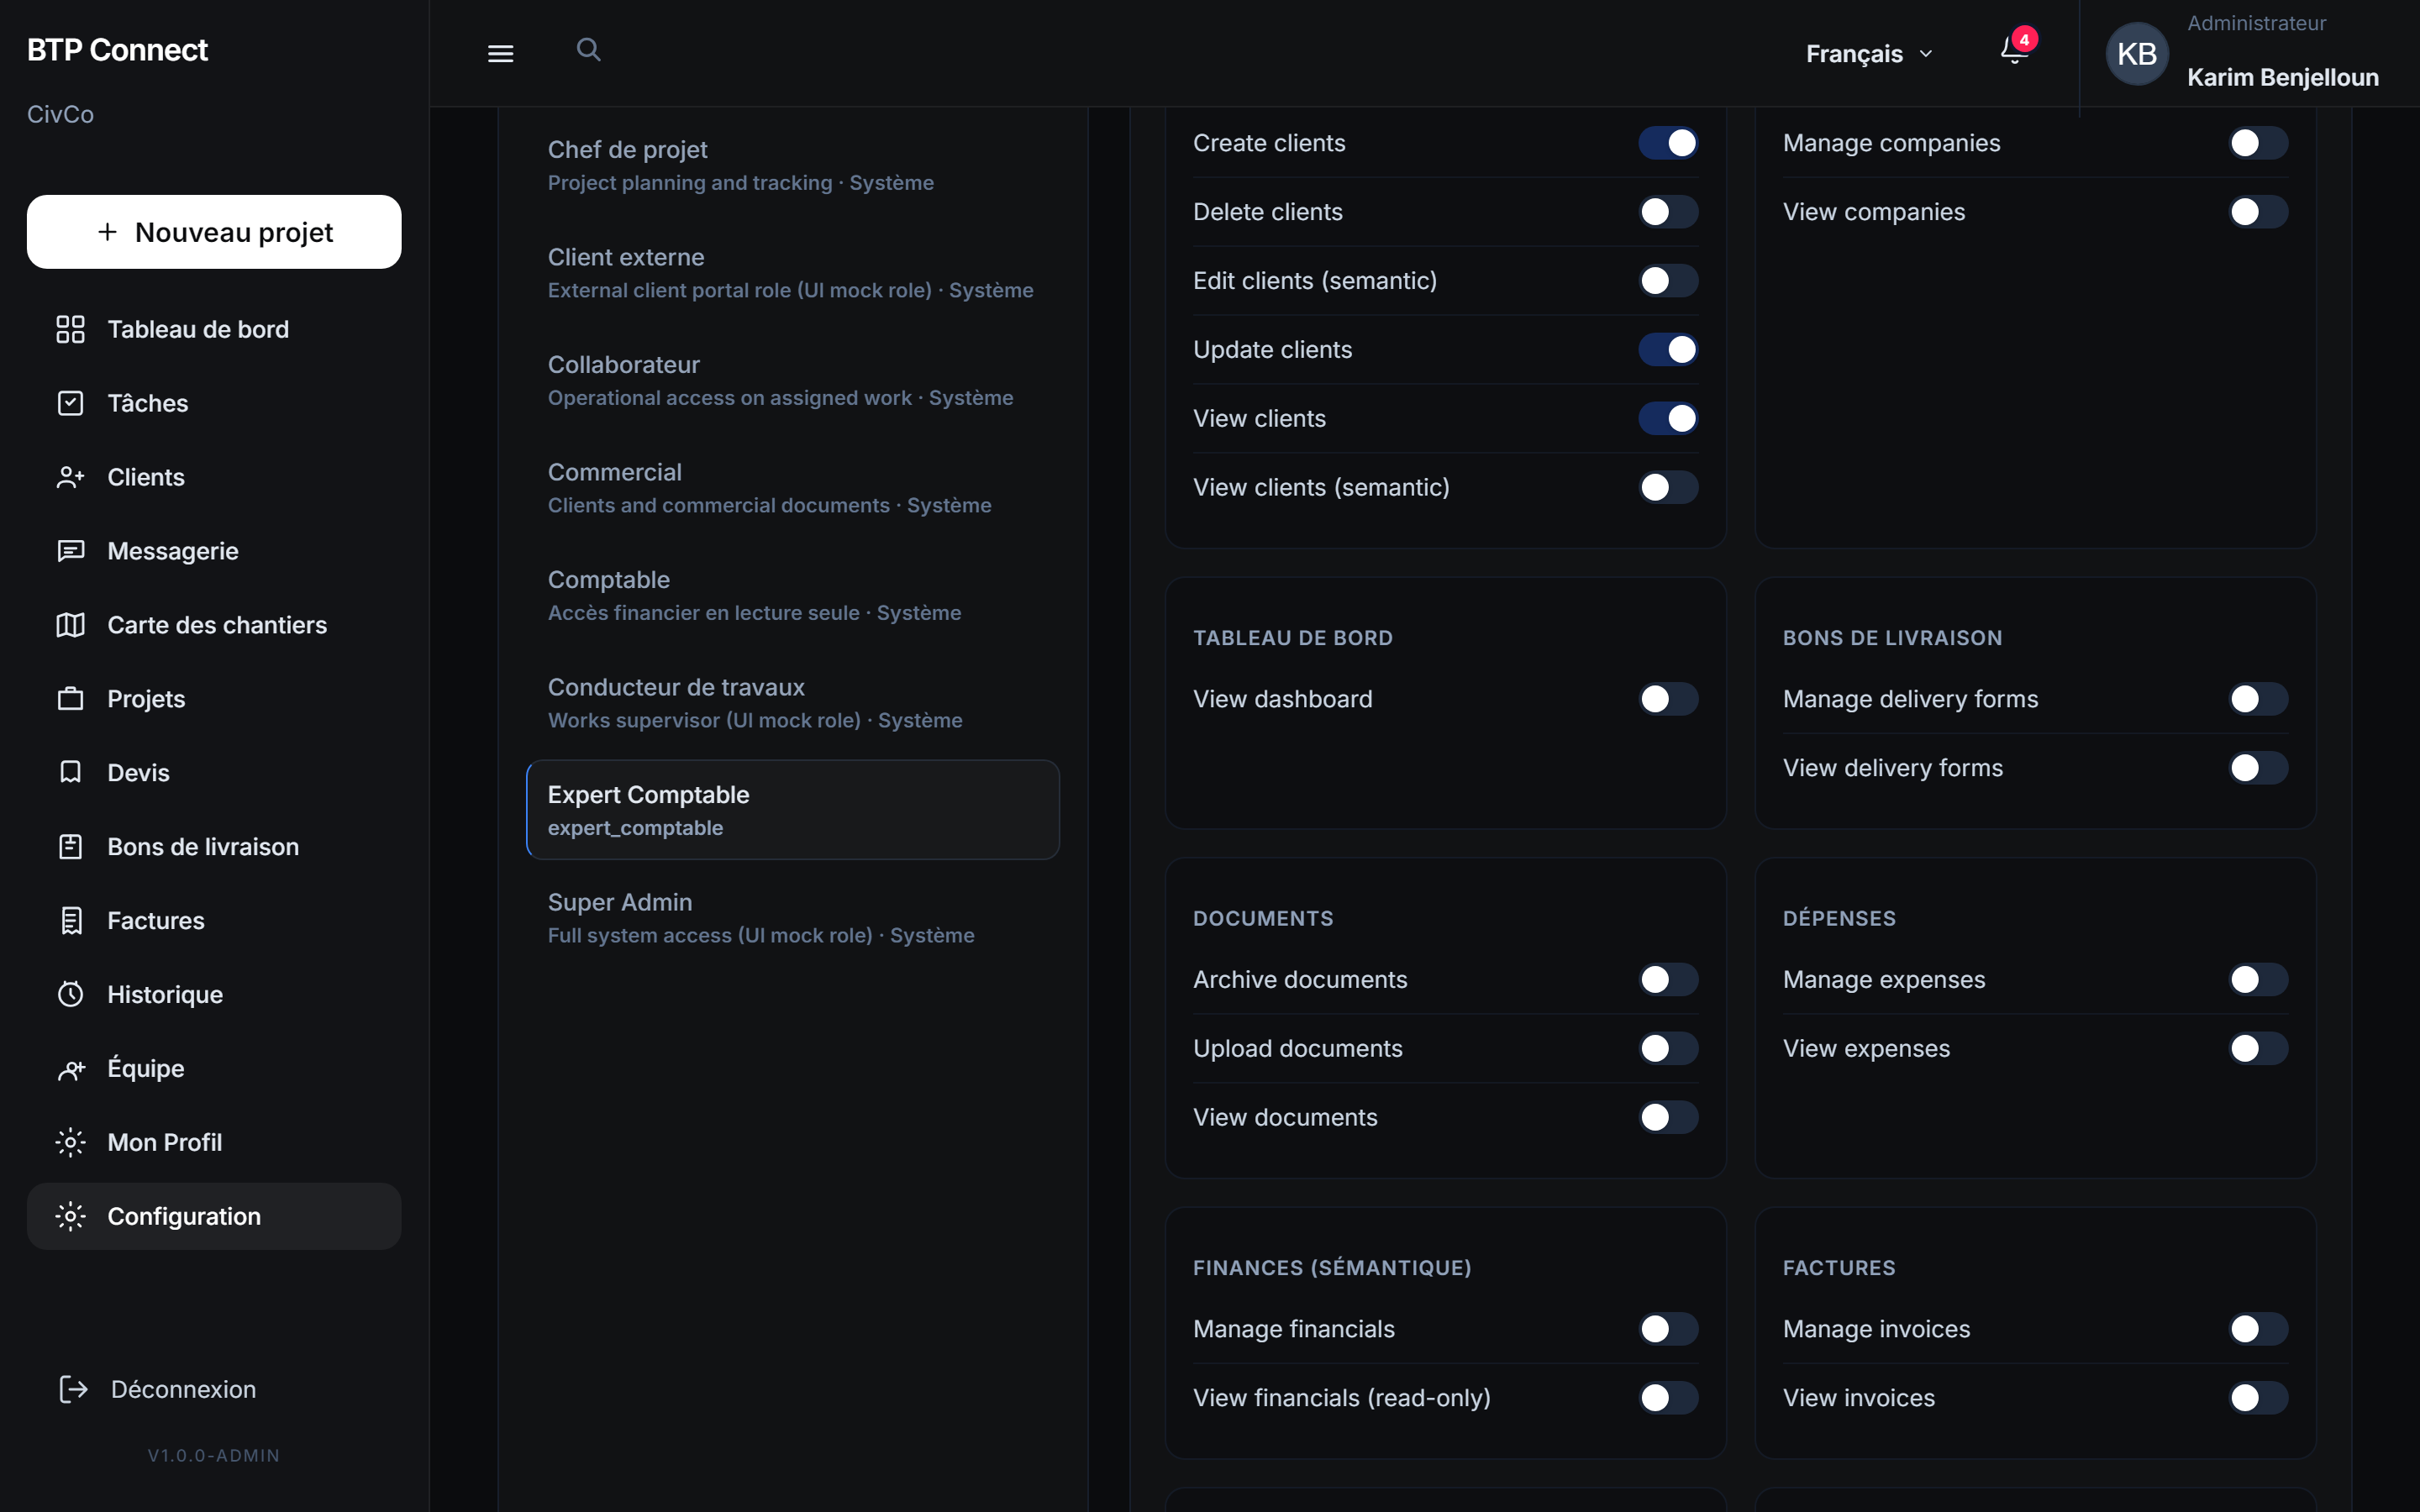
\includegraphics[width=\textwidth]{config.png}
  \caption{Module Configuration : rôles, modèles de documents, contrôles d'impression}
  \label{fig:config}
\end{figure}

Le module Configuration (Figure~\ref{fig:config}) est réservé à l'administrateur :
gestion des rôles et permissions, modèles de contrats et documents, paramètres
d'impression, thème visuel et référentiels (badges, lots, secteurs).

\medskip

Le panneau de configuration est organisé en onglets thématiques : rôles et permissions,
modèles de contrats, contrôles d'impression, modèles de documents et paramètres
généraux. L'administrateur peut créer un nouveau rôle métier, lui attribuer un
sous-ensemble de permissions et l'assigner aux utilisateurs concernés, sans
intervention technique sur le code.

% ─────────────────────────────────────────────────────────────────────
\section{Tests et validation}

La validation de l'application s'appuie sur deux dispositifs complémentaires : une
\textbf{suite de tests automatisés} PHPUnit au niveau du backend, et une
\textbf{campagne de tests manuels} couvrant les parcours utilisateurs de bout en bout.

\subsection{Tests automatisés backend}

Le projet inclut une suite de tests d'intégration PHPUnit dans \texttt{tests/Feature/} :

\begin{description}
  \item[AuthTest] Connexion, déconnexion, accès au profil utilisateur, rejet des
  identifiants invalides.
  \item[ClientProjectTest] CRUD clients et projets, relations, contraintes d'accès.
  \item[QuoteInvoiceTest] Création de devis, lignes de détail, conversion en facture,
  calcul des totaux.
  \item[DocumentTest] Upload et gestion des documents attachés aux projets.
  \item[ExpenseTest] Enregistrement des dépenses de chantier.
  \item[DashboardTest] Agrégation des indicateurs du tableau de bord.
  \item[RoleAccessTest] Vérification des redirections post-login et des permissions
  par profil (comptable, commercial, chef de projet, administrateur).
\end{description}

Les tests utilisent \texttt{RefreshDatabase} et les seeders de démonstration pour
garantir un environnement isolé et reproductible. La commande \texttt{php artisan test}
exécute l'ensemble de la suite.

\subsection{Campagne de tests manuels}

Une checklist de tests manuels a été établie pour valider les parcours que les tests
automatisés ne couvrent pas entièrement :

\begin{itemize}
  \item \textbf{Authentification} : connexion, déconnexion, expiration de session,
  redirection selon le profil.
  \item \textbf{Projets} : création complète (client, phases, équipe, géolocalisation),
  modification, consultation par un utilisateur non-admin.
  \item \textbf{Documents commerciaux} : cycle devis $\rightarrow$ acceptation $\rightarrow$
  facture $\rightarrow$ paiement ; impression avec et sans en-tête.
  \item \textbf{Contrats} : compilation depuis un modèle, signature portail client.
  \item \textbf{Tâches} : création, assignation, changement de statut, visibilité
  selon les permissions.
  \item \textbf{Portail client} : connexion client, consultation projet, acceptation
  devis, messagerie.
  \item \textbf{Configuration} : création de rôle, attribution de permissions,
  modification du thème.
  \item \textbf{Responsive} : consultation sur poste de bureau et tablette.
\end{itemize}

\subsection{Validation qualitative}

L'application a été validée en conditions réelles au sein de CIVCO BTP, avec les
observations suivantes :

\begin{itemize}
  \item \textbf{Adéquation métier} : les modules couvrent les processus quotidiens
  identifiés au Chapitre~1 (suivi de chantier, production documentaire, planification).
  \item \textbf{Ergonomie} : l'interface sombre et la navigation par sidebar ont été
  appréciées par les testeurs internes pour un usage prolongé.
  \item \textbf{Performance} : les listes et fiches détail se chargent en moins de
  500~ms en environnement local ; le tableau de bord agrège les indicateurs sans
  latence perceptible.
  \item \textbf{Sécurité} : les tests de contournement de permissions (accès direct
  à une URL sans droit) sont correctement bloqués côté API avec une réponse
  \texttt{403 Forbidden}.
  \item \textbf{Impression} : le mécanisme de suivi des copies officielles et le
  filigrane « COPIE - NON OFFICIEL » fonctionnent conformément aux exigences métier.
\end{itemize}

\subsection{Synthèse des tests}

Le Tableau~\ref{tab:test_summary} récapitule la couverture de validation par module.

\begin{table}[H]
\caption{Synthèse de la couverture de tests par module}
\label{tab:test_summary}
\centering
\small
\begin{tabular}{|l|c|c|p{5.5cm}|}
\hline
\textbf{Module} & \textbf{Auto.} & \textbf{Manuel} & \textbf{Points vérifiés} \\
\hline
Authentification & $\checkmark$ & $\checkmark$ & Login, logout, session, redirection \\
\hline
Projets & $\checkmark$ & $\checkmark$ & CRUD, phases, équipe, carte \\
\hline
Clients & $\checkmark$ & $\checkmark$ & CRUD, archivage, portail \\
\hline
Devis / Factures & $\checkmark$ & $\checkmark$ & Lignes, conversion, impression \\
\hline
Tâches & --- & $\checkmark$ & Assignation, statuts, permissions \\
\hline
Contrats & --- & $\checkmark$ & Compilation, signature, avenants \\
\hline
Configuration & --- & $\checkmark$ & Rôles, modèles, thème \\
\hline
Portail client & --- & $\checkmark$ & Consultation, acceptation, messagerie \\
\hline
\end{tabular}
\end{table}

% ─────────────────────────────────────────────────────────────────────
\section{Difficultés rencontrées et solutions}

\subsection{Gestion des permissions granulaires}

La mise en place du \textbf{RBAC} avec plus de trente permissions a nécessité une
coordination entre le backend (middleware, seeders) et le frontend (PermissionGate,
routePermissions). La solution retenue centralise la résolution des permissions
dans \texttt{AuthContextService} côté API et \texttt{permissionResolver.js} côté
React, garantissant une source de vérité unique.

\subsection{Impression documentaire}

La génération de PDF côté client (composants React dédiés) et le suivi des quotas
d'impression officielle ont demandé un mécanisme de comptage persistant
(\texttt{PrintTrackingService}) et une interface de choix avant chaque impression
(\texttt{PrintOptionsModal}).

\subsection{Géolocalisation des chantiers}

L'intégration de la carte Leaflet avec géocodage automatique des adresses de chantier
a été réalisée via \texttt{SiteGeocodingService}, qui interroge l'API Nominatim avec
un repli sur un référentiel de coordonnées des villes marocaines
(\texttt{MoroccoCityCoordinates}) en cas d'échec.

\subsection{Synchronisation frontend / backend}

La cohérence entre les permissions affichées dans l'interface et celles vérifiées
côté API a nécessité un travail de synchronisation : chaque route frontend dans
\texttt{routePermissions.js} doit correspondre à un contrôle \texttt{permission:*}
sur l'endpoint associé. Les tests \texttt{RoleAccessTest} et les tests manuels
multi-profils ont permis de détecter et corriger les écarts.

\section*{Conclusion}

Ce chapitre a présenté la réalisation concrète de l'application de gestion de
projets BTP développée pour CIVCO BTP. Au-delà de la conception formalisée au
chapitre précédent, nous avons décrit l'environnement d'exécution, l'organisation
du code, les modules livrés et les dispositifs de validation retenus pour garantir
la fiabilité de la solution en conditions d'usage réelles.

\medskip

\textbf{Environnement et architecture.} L'application repose sur une stack
\textbf{Laravel 13 / React 19 / Vite / MySQL}, orchestrée en développement par
deux processus parallèles (\texttt{php artisan serve} et \texttt{npm run dev}).
Le proxy Vite assure la communication transparente entre la SPA et l'API, tandis
que \textbf{Laravel Sanctum} gère l'authentification par session sécurisée.
Cette séparation frontend / backend a permis de maintenir une frontière nette :
l'interface React ne contient aucune règle métier critique ; la validation, les
calculs financiers et la persistance sont systématiquement assurés côté serveur.

\medskip

\textbf{Implémentation backend.} L'API REST expose plus de quarante contrôleurs
sous le préfixe \texttt{/api/v1/}, structurés par domaine (projets, clients,
devis, factures, tâches, contrats, configuration). Chaque endpoint sensible est
protégé par un middleware de permission (\texttt{permission:*}) et validé par
un Form Request dédié. Les services métier (\texttt{PrintTrackingService},
\texttt{DocumentTemplateCompilationService}, \texttt{TeamMemberService}, etc.)
centralisent les règles de gestion, tandis que les API Resources normalisent
les réponses JSON consommées par le frontend.

\medskip

\textbf{Interface utilisateur.} Le frontend React est organisé en modules par
domaine fonctionnel, avec une sidebar filtrée selon le profil connecté. Les
écrans principaux ont été implémentés et illustrés dans ce chapitre :
authentification (Figure~\ref{fig:login}), tableau de bord
(Figure~\ref{fig:dashboard}), gestion des projets et des clients
(Figures~\ref{fig:projects} et~\ref{fig:clients}), documents commerciaux
(Figures~\ref{fig:quotes} et~\ref{fig:invoices}), planification des tâches
(Figure~\ref{fig:tasks}), carte géographique des chantiers (Figure~\ref{fig:map}),
portail client (Figure~\ref{fig:portal}) et module de configuration
(Figure~\ref{fig:config}). Cette couverture correspond au périmètre fonctionnel
défini au Chapitre~3 et aux processus quotidiens de CIVCO BTP.

\medskip

\textbf{Validation et déploiement.} La qualité de la solution est assurée par
une suite de tests PHPUnit (authentification, CRUD métier, conversion
devis $\rightarrow$ facture, contrôle d'accès par rôle) complétée par une
campagne de tests manuels sur les parcours de bout en bout. L'étude comparative
d'hébergement a orienté le choix vers \textbf{o2switch}, retenu pour sa simplicité
de mise en production, son support francophone et son rapport qualité/prix adapté
à une PME du secteur BTP.

\medskip

\textbf{Bilan.} Les principales difficultés --- permissions granulaires,
impression documentaire, géolocalisation des chantiers et synchronisation
frontend / backend --- ont été résolues par des services dédiés et une
source de vérité unique côté API. L'application est fonctionnelle, testée et
prête pour un déploiement chez CIVCO BTP. Le chapitre suivant conclut ce rapport
en synthétisant les apports du projet et en esquissant les perspectives
d'évolution (notifications temps réel, application mobile, intégration comptable).

\newpage

% \chapter*{Conclusion Générale et Perspectives}
\addcontentsline{toc}{chapter}{Conclusion Générale et Perspectives}
\markboth{Conclusion Générale et Perspectives}{Conclusion Générale et Perspectives}

Ce projet de fin d'études avait pour objectif de concevoir et développer une
application web de gestion et de planification des projets de construction pour
\textbf{CIVCO BTP}, afin de centraliser les processus métier dispersés entre
tableurs, documents papier et échanges informels.

\medskip

L'application développée au cours de ce stage constitue une réponse concrète et
fonctionnelle à cette problématique. Les réalisations techniques couvrent
l'intégralité du cycle de vie d'un projet de construction :

\begin{itemize}
  \item \textbf{Gestion de projets} : création et suivi des chantiers par phases,
  affectation des équipes, géolocalisation sur carte interactive, suivi de
  l'avancement et des dépenses.
  \item \textbf{Relation client} : fiches clients centralisées, archivage, portail
  dédié pour consultation et validation des documents.
  \item \textbf{Documents commerciaux} : production de devis, factures et bons de
  livraison avec lignes de détail, conversion automatisée et suivi des impressions
  officielles.
  \item \textbf{Suivi contractuel} : gestion des contrats et avenants, compilation
  depuis des modèles, signature électronique côté client.
  \item \textbf{Planification opérationnelle} : tâches assignées par projet et par
  collaborateur, tableau de bord avec indicateurs et graphiques.
  \item \textbf{Sécurité et gouvernance} : authentification Sanctum, contrôle
  d'accès par rôles et permissions (RBAC), journal d'activité pour la traçabilité.
  \item \textbf{Architecture technique} : backend Laravel 13 exposant une API REST,
  frontend React 19 en SPA, base de données relationnelle, plus de soixante-dix
  migrations et une suite de tests PHPUnit.
\end{itemize}

\section*{Bilan du projet}

Sur le plan fonctionnel, l'application répond aux besoins identifiés lors de la
phase d'analyse : chaque service de CIVCO BTP dispose désormais d'un point d'accès
unique pour consulter et mettre à jour les informations liées aux chantiers. La
centralisation des données élimine les ressaisies manuelles entre tableurs et
documents isolés, et le tableau de bord offre une visibilité en temps réel sur
l'activité de l'entreprise.

\medskip

Sur le plan technique, les choix Laravel + React se sont révélés pertinents pour
ce type d'application métier : Laravel fournit une base solide pour l'API, la
sécurité et la persistance, tandis que React permet de construire une interface
réactive et modulaire. L'architecture en trois couches facilite la maintenance
et l'ajout de nouveaux modules sans remettre en cause l'existant.

\medskip

Sur le plan méthodologique, l'approche itérative adoptée pendant le stage ---
analyse des besoins, conception, développement par modules, tests et validation
--- a permis de livrer des incréments fonctionnels démontrables à chaque réunion
de suivi avec l'encadrant professionnel, M. Mohamed BENABDELLAH-CHAOUNI, et
l'encadrant pédagogique, le Pr. Mohammed El Assad.

\section*{Apports personnels et compétences acquises}

Ce stage au sein de CIVCO BTP m'a permis de consolider et d'approfondir
plusieurs compétences techniques et transversales :

\begin{itemize}
  \item \textbf{Développement full-stack} : conception et implémentation d'une
  application complète, de la base de données à l'interface utilisateur.
  \item \textbf{Architecture logicielle} : application des patrons MVC, services
  métier, API REST et SPA dans un contexte professionnel réel.
  \item \textbf{Sécurité applicative} : mise en œuvre concrète de l'authentification,
  du RBAC, de la protection CSRF et de la journalisation.
  \item \textbf{Modélisation} : rédaction de spécifications fonctionnelles,
  diagrammes UML et modèle de données relationnel.
  \item \textbf{Gestion de projet} : planification, priorisation des fonctionnalités,
  suivi Kanban via Trello, communication régulière avec les parties prenantes.
  \item \textbf{Rigueur documentaire} : rédaction du présent rapport et documentation
  technique du code produit.
\end{itemize}

\medskip

Au-delà des compétences techniques, ce projet m'a sensibilisé aux réalités du
secteur BTP au Maroc : la diversité des intervenants sur un chantier, l'importance
de la traçabilité documentaire et les contraintes de terrain qui influencent les
choix ergonomiques de l'application.

\section*{Limites et axes d'amélioration}

Malgré les résultats obtenus, certaines limites subsistent et ouvrent des pistes
d'amélioration :

\begin{itemize}
  \item \textbf{Couverture de tests} : la suite PHPUnit couvre les flux critiques
  mais ne teste pas encore l'ensemble des modules (contrats, portail client).
  L'ajout de tests end-to-end (Cypress, Playwright) renforcerait la confiance
  avant un déploiement en production.
  \item \textbf{Performance à l'échelle} : les tests ont été réalisés en
  environnement local avec un volume de données modéré. Un benchmark sur des
  milliers de projets et documents serait nécessaire avant un usage intensif.
  \item \textbf{Formation utilisateurs} : l'adoption de l'outil par l'ensemble des
  services nécessitera un accompagnement au changement et une documentation
  utilisateur dédiée.
  \item \textbf{Déploiement production} : une étude comparative OVHcloud / o2switch a
  conduit au choix d'\textbf{o2switch} ; la mise en ligne effective reste à finaliser
  (configuration du domaine, déploiement du build React et exécution des migrations).
\end{itemize}

\section*{Perspectives}

L'application offre plusieurs pistes d'évolution à court et moyen terme pour CIVCO BTP.

\medskip

\textbf{Évolutions fonctionnelles :}
\begin{itemize}
  \item \textbf{Application mobile} : version allégée pour les conducteurs de travaux
  sur chantier (consultation des tâches, mise à jour d'avancement, photos).
  \item \textbf{Business Intelligence} : tableaux de bord avancés, export Excel/PDF
  des indicateurs, analyse de la rentabilité par projet.
  \item \textbf{Gestion des stocks} : suivi des matériaux et approvisionnements liés
  aux chantiers.
  \item \textbf{Notifications} : alertes email ou push pour les échéances de tâches,
  validations en attente et paiements.
  \item \textbf{Signature avancée} : intégration d'un prestataire de signature
  électronique qualifiée pour les contrats à forte valeur juridique.
\end{itemize}

\textbf{Évolutions techniques :}
\begin{itemize}
  \item \textbf{Déploiement production (o2switch)} : publication de l'application sur
  l'hébergement retenu (build React, configuration Laravel, certificat SSL, sauvegardes
  automatiques de la base MySQL).
  \item \textbf{Montée en charge} : si le volume d'utilisateurs augmente significativement,
  migration vers une offre VPS OVHcloud ou cloud managé pour plus de flexibilité.
  \item \textbf{Tests} : extension de la couverture PHPUnit, ajout de tests
  end-to-end (Cypress ou Playwright) sur les parcours critiques.
  \item \textbf{Performance} : mise en cache des requêtes fréquentes (Redis),
  pagination optimisée sur les grandes listes.
  \item \textbf{CI/CD} : pipeline d'intégration continue (GitHub Actions) pour
  exécuter les tests automatiquement à chaque commit.
\end{itemize}

\medskip

Ce projet illustre comment une architecture web moderne (Laravel + React) peut
transformer la gestion quotidienne d'une entreprise du BTP, en remplaçant des outils
dispersés par une plateforme intégrée, sécurisée et adaptée aux profils métier de
l'organisation. L'application constitue une base solide sur laquelle CIVCO BTP peut
continuer à digitaliser et optimiser ses processus internes, au service de la qualité
de ses études et du suivi de ses chantiers.

\newpage


% \nocite{*}
% \printbibliography[heading=bibintoc, title={Bibliographie et Webographie}]
% \newpage

% \appendix
% % ─────────────────────────────────────────────────────────────────────
%   ANNEXES
% ─────────────────────────────────────────────────────────────────────

% Configuration globale des listings de code
\lstset{
  basicstyle=\ttfamily\footnotesize,
  breaklines=true,
  breakatwhitespace=false,
  columns=fullflexible,
  keepspaces=true,
  showstringspaces=false,
  tabsize=2,
  frame=single,
  rulecolor=\color{ensamBlue!40},
  backgroundcolor=\color{ensamBlue!3},
  xleftmargin=0.5cm,
  xrightmargin=0.5cm,
  keywordstyle=\color{ensamBlue}\bfseries,
  stringstyle=\color{orange!70!black},
  commentstyle=\color{gray}\itshape,
  numberstyle=\tiny\color{gray},
  numbers=left,
  numbersep=6pt,
  captionpos=b,
}

\chapter{Annexes}

% =====================================================================
\section{Extraits de code source}

Cette annexe présente les extraits de code source les plus représentatifs de
l'application développée pour CIVCO BTP, sélectionnés pour illustrer les
contributions techniques décrites dans ce rapport.

% ─────────────────────────────────────────────────────────────────────
\subsection{Authentification API (\texttt{AuthController.php})}

Le contrôleur d'authentification gère la connexion des utilisateurs internes
via Laravel Sanctum. La méthode \texttt{login} valide les identifiants, régénère
la session et retourne le contexte utilisateur (profil, rôles, permissions).

\begin{lstlisting}[language=PHP,
  caption={AuthController.php : connexion utilisateur (extrait)}]
public function login(LoginRequest $request,
    AuthContextService $authContext): JsonResponse
{
    $credentials = $request->only('email', 'password');

    if (! Auth::attempt($credentials, $request->boolean('remember'))) {
        throw ValidationException::withMessages([
            'email' => [__('auth.failed')],
        ]);
    }

    $user = Auth::user();

    if (! $user->canAccessApplication()) {
        Auth::logout();
        throw ValidationException::withMessages([
            'email' => [CheckUserStatus::DEACTIVATED_MESSAGE],
        ]);
    }

    if ($request->hasSession()) {
        $request->session()->regenerate();
    }

    return response()->json($authContext->forUser($user));
}
\end{lstlisting}

% ─────────────────────────────────────────────────────────────────────
\subsection{Conversion devis vers facture (\texttt{QuoteService.php})}

Le service métier \texttt{QuoteService} encapsule la logique de conversion d'un
devis accepté en facture. L'opération s'exécute dans une transaction base de
données pour garantir la cohérence des enregistrements.

\begin{lstlisting}[language=PHP,
  caption={QuoteService.php : conversion devis $\rightarrow$ facture (extrait)}]
public function convertToInvoice(Quote $quote,
    ?int $dispatchNoteId = null): Invoice
{
    if ($quote->status !== QuoteStatus::Accepted) {
        throw new InvalidArgumentException(
            'Only accepted quotes can be converted.');
    }

    if ($quote->invoice()->exists()) {
        throw new InvalidArgumentException(
            'This quote has already been converted.');
    }

    return DB::transaction(function () use ($quote, $dispatchNoteId) {
        $quote->load('lines');

        $invoice = Invoice::query()->create([
            'company_id' => $quote->company_id,
            'client_id'  => $quote->client_id,
            'project_id' => $quote->project_id,
            'quote_id'   => $quote->id,
            'reference'  => $this->invoiceReferenceService
                                ->nextForCompany($quote->company_id),
            'status'     => InvoiceStatus::Draft,
            'total_ht'   => $quote->total_ht,
            'total_tax'  => $quote->total_tax,
            'total_ttc'  => $quote->total_ttc,
        ]);

        foreach ($quote->lines as $index => $line) {
            $invoice->lines()->create([
                'sort_order'      => $index + 1,
                'description'     => $line->description,
                'quantity'        => $line->quantity,
                'unit_price_ht'   => $line->unit_price_ht,
                'line_total_ht'   => $line->line_total_ht,
                'line_total_ttc'  => $line->line_total_ttc,
            ]);
        }

        return $invoice->load(['client', 'project', 'lines']);
    });
}
\end{lstlisting}

% ─────────────────────────────────────────────────────────────────────
\subsection{Modèle Projet (\texttt{Project.php})}

Le modèle Eloquent \texttt{Project} centralise les relations métier d'un chantier :
client, phases, équipe, devis et factures.

\begin{lstlisting}[language=PHP,
  caption={Project.php : relations Eloquent (extrait)}]
class Project extends Model
{
    protected $fillable = [
        'company_id', 'client_id', 'reference', 'title',
        'status', 'budget', 'progress_percent',
        'start_date', 'end_date', 'latitude', 'longitude',
    ];

    protected function casts(): array
    {
        return [
            'status' => ProjectStatus::class,
            'start_date' => 'date',
            'end_date' => 'date',
            'budget' => 'decimal:2',
            'progress_percent' => 'decimal:2',
        ];
    }

    public function client(): BelongsTo
    {
        return $this->belongsTo(Client::class);
    }

    public function phases(): HasMany
    {
        return $this->hasMany(ProjectPhase::class);
    }

    public function teamMembers(): BelongsToMany
    {
        return $this->belongsToMany(User::class, 'project_user');
    }

    public function quotes(): HasMany
    {
        return $this->hasMany(Quote::class);
    }
}
\end{lstlisting}

% ─────────────────────────────────────────────────────────────────────
\subsection{Client HTTP frontend (\texttt{client.js})}

Le module \texttt{api/client.js} configure l'instance Axios partagée par tous
les modules frontend. Il transmet les cookies Sanctum, le jeton CSRF et le
contexte société (\texttt{X-Company-Id}).

\begin{lstlisting}[language=Java,
  caption={client.js : configuration Axios et intercepteurs (extrait)}]
const api = axios.create({
  baseURL: import.meta.env.VITE_API_URL ?? '',
  withCredentials: true,
  headers: {
    Accept: 'application/json',
    'Content-Type': 'application/json',
    'X-Requested-With': 'XMLHttpRequest',
  },
})

api.interceptors.request.use(async (config) => {
  if (activeCompanyId) {
    config.headers['X-Company-Id'] = activeCompanyId
  }

  const method = config.method?.toLowerCase()
  if (['post', 'put', 'patch', 'delete'].includes(method)) {
    let token = getCookie('XSRF-TOKEN')
    if (!token) {
      await api.get('/sanctum/csrf-cookie')
      token = getCookie('XSRF-TOKEN')
    }
    if (token) {
      config.headers['X-XSRF-TOKEN'] = token
    }
  }

  return config
})

api.interceptors.response.use(
  (response) => response,
  (error) => {
    if (error.response?.status === 401) {
      window.dispatchEvent(new CustomEvent('auth:unauthorized'))
    }
    return Promise.reject(error)
  }
)
\end{lstlisting}

% =====================================================================
\section{Configuration : variables d'environnement}

Le fichier \texttt{.env} du backend centralise la configuration de l'application.
Le Tableau~\ref{tab:annexe_env} décrit les variables principales utilisées en
développement et en production.

\begin{table}[H]
\caption{Variables d'environnement principales}
\label{tab:annexe_env}
\centering
\small
\begin{tabular}{|l|p{8.5cm}|}
\hline
\textbf{Variable} & \textbf{Rôle} \\
\hline
\texttt{APP\_URL} & URL publique du backend Laravel \\
\hline
\texttt{DB\_CONNECTION} & Pilote SGBD (\texttt{mysql} ou \texttt{pgsql}) \\
\hline
\texttt{DB\_DATABASE} & Nom de la base de données \\
\hline
\texttt{SESSION\_DRIVER} & Stockage des sessions (\texttt{database} recommandé) \\
\hline
\texttt{SANCTUM\_STATEFUL\_DOMAINS} & Domaines autorisés pour les cookies SPA \\
\hline
\texttt{FRONTEND\_URL} & URL du frontend React (CORS et redirections) \\
\hline
\texttt{MAIL\_*} & Configuration SMTP pour les notifications \\
\hline
\end{tabular}
\end{table}

\medskip

Exemple de configuration minimale pour un environnement de développement local :

\lstset{
  language={},
  keywordstyle=\color{black},
  stringstyle=\color{black},
  commentstyle=\color{gray}\itshape,
}

\begin{lstlisting}[caption={.env : configuration de développement (extrait)}]
APP_NAME="CIVCO BTP"
APP_ENV=local
APP_DEBUG=true
APP_URL=http://127.0.0.1:8000

DB_CONNECTION=mysql
DB_HOST=127.0.0.1
DB_PORT=3306
DB_DATABASE=civco_btp
DB_USERNAME=root
DB_PASSWORD=

SESSION_DRIVER=database
SESSION_LIFETIME=120

SANCTUM_STATEFUL_DOMAINS=localhost,127.0.0.1:5173

FRONTEND_URL=http://127.0.0.1:5173

MAIL_MAILER=smtp
MAIL_HOST=smtp.example.com
MAIL_PORT=587
MAIL_USERNAME=null
MAIL_PASSWORD=null
\end{lstlisting}

% =====================================================================
\section{Comptes de démonstration}

Le seeder de démonstration fournit des comptes utilisateurs permettant de
tester les différents profils métier de CIVCO BTP. Le Tableau~\ref{tab:demo_users}
liste les identifiants utilisés en environnement de développement.

\begin{table}[H]
\caption{Comptes de démonstration (mot de passe : \texttt{password})}
\label{tab:demo_users}
\centering
\small
\begin{tabular}{|l|l|p{5.5cm}|}
\hline
\textbf{Email} & \textbf{Profil} & \textbf{Accès principal} \\
\hline
\texttt{admin@civco.ma} & Administrateur & Configuration, tous modules \\
\hline
\texttt{ingenieur@civco.ma} & Chef de projet & Projets, tâches, équipe \\
\hline
\texttt{compta@civco.ma} & Comptable & Factures, paiements \\
\hline
\texttt{chantier@civco.ma} & Chef de chantier & Projets, tâches terrain \\
\hline
\texttt{tech@civco.ma} & Technicien & Tâches assignées, consultation \\
\hline
\end{tabular}
\end{table}

\medskip

Ces comptes sont créés par la commande \texttt{php artisan migrate --seed} et
permettent de valider le contrôle d'accès par rôles décrit au Chapitre~3.

% =====================================================================
\section{Référentiel des endpoints API}

Le Tableau~\ref{tab:api_endpoints} présente les principaux endpoints exposés
sous le préfixe \texttt{/api/v1/}. Toutes les routes (sauf \texttt{login}) sont
protégées par le middleware \texttt{auth:sanctum} et soumises à un contrôle de
permissions.

\begin{table}[H]
\caption{Principaux endpoints de l'API REST}
\label{tab:api_endpoints}
\centering
\footnotesize
\begin{tabular}{|l|l|p{5.5cm}|}
\hline
\textbf{Méthode} & \textbf{Endpoint} & \textbf{Description} \\
\hline
POST & \texttt{/login} & Authentification utilisateur \\
\hline
GET & \texttt{/me} & Profil et permissions de l'utilisateur courant \\
\hline
GET/POST & \texttt{/projects} & Liste et création de projets \\
\hline
GET/PUT & \texttt{/projects/\{id\}} & Consultation et modification d'un projet \\
\hline
GET/POST & \texttt{/clients} & Liste et création de clients \\
\hline
GET/POST & \texttt{/quotes} & Liste et création de devis \\
\hline
POST & \texttt{/quotes/\{id\}/convert} & Conversion devis $\rightarrow$ facture \\
\hline
GET/POST & \texttt{/invoices} & Liste et création de factures \\
\hline
GET/POST & \texttt{/tasks} & Liste et création de tâches \\
\hline
GET/POST & \texttt{/contracts} & Liste et création de contrats \\
\hline
GET & \texttt{/dashboard} & Indicateurs du tableau de bord \\
\hline
GET & \texttt{/search} & Recherche globale (clients, projets, documents) \\
\hline
GET & \texttt{/activity-logs} & Journal des actions (administrateur) \\
\hline
\end{tabular}
\end{table}

% =====================================================================
\section{Schéma des entités principales}

Le Tableau~\ref{tab:entity_schema} décrit les attributs essentiels des entités
métier les plus consultées dans l'application.

\begin{table}[H]
\caption{Attributs principaux des entités métier}
\label{tab:entity_schema}
\centering
\small
\begin{tabular}{|l|p{10.5cm}|}
\hline
\textbf{Entité} & \textbf{Attributs clés} \\
\hline
\texttt{Project} & \texttt{reference}, \texttt{title}, \texttt{status}, \texttt{budget},
\texttt{progress\_percent}, \texttt{start\_date}, \texttt{end\_date},
\texttt{latitude}, \texttt{longitude}, \texttt{client\_id} \\
\hline
\texttt{Client} & \texttt{name}, \texttt{email}, \texttt{phone}, \texttt{status},
\texttt{is\_official}, \texttt{archived\_at} \\
\hline
\texttt{Quote} & \texttt{reference}, \texttt{status}, \texttt{total\_ht},
\texttt{total\_tax}, \texttt{total\_ttc}, \texttt{project\_id}, \texttt{client\_id} \\
\hline
\texttt{Invoice} & \texttt{reference}, \texttt{status}, \texttt{issued\_at},
\texttt{due\_date}, \texttt{amount\_paid}, \texttt{balance\_due}, \texttt{quote\_id} \\
\hline
\texttt{Task} & \texttt{title}, \texttt{status}, \texttt{priority},
\texttt{due\_date}, \texttt{project\_phase\_id}, \texttt{assigned\_to} \\
\hline
\texttt{Contract} & \texttt{reference}, \texttt{status}, \texttt{signed\_at},
\texttt{project\_id}, \texttt{template\_id} \\
\hline
\end{tabular}
\end{table}

\medskip

Les statuts des entités sont implémentés sous forme d'énumérations PHP
(\texttt{ProjectStatus}, \texttt{QuoteStatus}, \texttt{InvoiceStatus},
\texttt{TaskStatus}) garantissant la validité des transitions d'état côté
serveur.

% =====================================================================
\section{Guide de démarrage rapide}

Pour reproduire l'environnement de développement décrit au Chapitre~4, les commandes
suivantes permettent d'initialiser l'application à partir du dépôt source :

\begin{lstlisting}[language={}, caption={Commandes d'initialisation de l'application}]
# Backend
cd backend
composer install
cp .env.example .env
php artisan key:generate
php artisan migrate --seed
php artisan serve

# Frontend (dans un second terminal)
cd frontend
npm install
npm run dev
\end{lstlisting}

\medskip

L'application est alors accessible à l'adresse \texttt{http://127.0.0.1:5173} (frontend)
avec le proxy Vite redirigeant les appels API vers \texttt{http://127.0.0.1:8000}.
Les comptes de démonstration listés en section~3 permettent de tester les différents
profils métier.

\newpage


% \end{document}




% ============================================================
%   RAPPORT DE FIN D'ÉTUDES — EMSI CASABLANCA — FILIÈRE IIR
%   Compiler: xelatex main.tex
% ============================================================

\documentclass[12pt, a4paper]{report}

% ── 1. Maths ─────────────────────────────────────────────────
\usepackage{amsmath, amssymb}

% ── 2. Font engine ───────────────────────────────────────────
\usepackage{fontspec}

% ── 3. All packages ──────────────────────────────────────────
\usepackage[top=2.5cm, bottom=2.5cm, left=3cm, right=2.5cm]{geometry}
\usepackage{setspace}
\usepackage[dvipsnames]{xcolor}
\usepackage{graphicx}
\usepackage{float}
\usepackage{booktabs}
\usepackage{tabularx}
\usepackage{array}
\usepackage{multirow}
\usepackage{multicol}
\usepackage{listings}
\usepackage{tcolorbox}
\usepackage{caption}
\usepackage{csquotes}
\usepackage[titles]{tocloft}
\usepackage{fancyhdr}
\usepackage{chngcntr}
\usepackage{tikz}
\usetikzlibrary{arrows.meta, shapes.geometric, positioning, fit, backgrounds, calc, shadows}

% ── 4. polyglossia — French + English only (no Arabic here) ──
%     Adding Arabic via polyglossia auto-loads bidi, which then
%     conflicts with biblatex. We load bidi manually below.
\usepackage{polyglossia}
\setmainlanguage{french}
\setotherlanguage{english}
\setmainfont{Times New Roman}
\newfontfamily\arabicfont[Script=Arabic, Scale=1.1]{Amiri}

% ── 5. biblatex after polyglossia ────────────────────────────
\usepackage[backend=biber, style=ieee]{biblatex}
\addbibresource{references.bib}

% ── 6. hyperref before bidi ──────────────────────────────────
\usepackage[colorlinks=true, linkcolor=black, citecolor=black, urlcolor=blue,
  pdfauthor={Othmane BENHRADDI},
  pdftitle={Rapport PFE - EMSI Casablanca 2026 - Gestion et Planification Projets BTP}]{hyperref}

% ── 7. bidi manually last — all packages already loaded ──────
\usepackage{bidi}
\newenvironment{arabicblock}{\begin{RTL}\arabicfont\relax}{\end{RTL}}

% ── Inline tech logo helper ──────────────────────────────────
\newcommand{\techlogo}[1]{\raisebox{-0.4ex}{\includegraphics[height=1.8em]{#1}}\;}
\providecommand{\screenshotplaceholder}[1]{%
  \fbox{\parbox{0.92\textwidth}{\centering\vspace{2.6cm}%
  \textit{#1}\\[0.2cm]{\footnotesize Capture d'écran à insérer}%
  \vspace{2.6cm}}}%
}

% ── Line-break tolerance (prevents overfull hbox) ────────────
\setlength{\emergencystretch}{3em}
\tolerance=500
\hbadness=500

% ── Settings ─────────────────────────────────────────────────
\onehalfspacing
\graphicspath{{img/}}
\captionsetup[figure]{name=Figure, labelsep=colon}
\captionsetup[table]{name=Tableau, labelsep=colon, position=above}
\counterwithin{figure}{chapter}
\counterwithin{table}{chapter}
\setlength{\headheight}{14.5pt}
\addtolength{\topmargin}{-0.5pt}
\pagestyle{fancy}
\fancyhf{}
\fancyhead[L]{\small\leftmark}
\fancyhead[R]{\small EMSI Casablanca, 2025/2026}
\fancyfoot[C]{\thepage}
\renewcommand{\headrulewidth}{0.4pt}
\definecolor{ensamBlue}{RGB}{0, 70, 127}

% ── Chapter titles: « Chapitre N : Titre » ───────────────────
\makeatletter
\renewcommand{\@makechapterhead}[1]{%
  \vspace*{50\p@}%
  {\parindent \z@ \raggedright \normalfont
    \ifnum \c@secnumdepth >\m@ne
      \Huge\bfseries Chapitre~\thechapter~: #1\par\nobreak
      \vskip 40\p@
    \else
      \Huge\bfseries #1\par\nobreak
      \vskip 40\p@
    \fi
  }}
\makeatother
\renewcommand{\cftchappresnum}{Chapitre~}
\renewcommand{\cftchapaftersnum}{~:}
\setlength{\cftchapnumwidth}{5em}

% Compact headings for \chapter* (Résumé, Abstract, Dédicaces, etc.)
\makeatletter
\renewcommand{\@makeschapterhead}[1]{%
  \vspace*{8\p@}%
  {\parindent \z@ \raggedright \normalfont
    \interlinepenalty\@M
    \Huge \bfseries #1\par\nobreak
    \vskip 14\p@
  }}
\makeatother

% ============================================================
\begin{document}

% ── Front matter (roman numerals) ───────────────────────────
\pagenumbering{roman}
\setcounter{page}{0}
\raggedbottom

% ============================================================
%  00 - Page de garde (template EMSI / Honoris — layout officiel)
%  Logos :
%    - img/emsi_cover.png  (extrait du template, déjà en place)
%    - img/civco_cover.png (à ajouter pour remplacer le placeholder)
% ============================================================

\definecolor{emsiGreen}{RGB}{0, 175, 80}
\definecolor{emsiGreenDark}{RGB}{45, 124, 82}
\definecolor{emsiRowBg}{RGB}{241, 247, 244}
\definecolor{emsiNameBar}{RGB}{213, 238, 224}
\definecolor{emsiTitleGray}{RGB}{70, 70, 70}
\definecolor{emsiMuted}{RGB}{100, 100, 100}
\definecolor{emsiBoxBorder}{RGB}{170, 170, 170}

\newfontfamily\coverSans{Arial}

\newcommand{\coverlabel}[1]{%
  {\coverSans\scriptsize\bfseries\color{emsiGreenDark}#1}\par\vspace{0.06cm}%
}
\newcommand{\covername}[1]{%
  \noindent
  \colorbox{emsiNameBar}{%
    \parbox{\dimexpr\linewidth-2\fboxsep\relax}{%
      \centering\vspace{0.1cm}%
      {\coverSans\small\bfseries\itshape\color{emsiGreenDark}#1}%
      \vspace{0.1cm}%
    }%
  }\par\vspace{0.18cm}%
}

\newgeometry{top=1.1cm, bottom=1.2cm, left=1.5cm, right=1.5cm}

\begin{titlepage}
  \thispagestyle{empty}
  \setlength{\parindent}{0pt}

  % Triangles verts (coins)
  \begin{tikzpicture}[remember picture, overlay]
    \fill[emsiGreen]
      (current page.north west) -- ++(0,-6.6cm) -- ++(6.6cm,6.6cm) -- cycle;
    \fill[emsiGreen]
      (current page.south east) -- ++(0,4.2cm) -- ++(-4.2cm,-4.2cm) -- cycle;
    \draw[emsiMuted!40, line width=0.5pt]
      ([yshift=1.7cm]current page.south west)
      -- ([yshift=1.7cm]current page.south east);
  \end{tikzpicture}

  % Logo EMSI — haut droite
  \noindent\hfill
  \IfFileExists{img/emsi_cover.png}{%
    
\includegraphics[width=0.52\textwidth]{emsi_cover.png}%
  }{%
    \begin{minipage}{0.52\textwidth}\raggedleft
      {\coverSans\color{emsiGreenDark}\bfseries\fontsize{9}{11}\selectfont
        ECOLE MAROCAINE DES SCIENCES DE L'INGENIEUR\par}
      {\coverSans\color{emsiMuted}\fontsize{7}{9}\selectfont
        Membre de HONORIS UNITED UNIVERSITIES\par}
    \end{minipage}%
  }

  \vspace{0.7cm}

  \begin{center}
    {\fontsize{22}{25}\selectfont\bfseries FINAL-YEAR\par}
    \vspace{0.05cm}
    {\fontsize{26}{29}\selectfont\bfseries PROJECT REPORT\par}
    \vspace{0.28cm}
    {\coverSans\fontsize{10.5}{12}\selectfont
      Program: Computer and Network Engineering (IIR), 5th year\par}
  \end{center}

  \vspace{0.55cm}

  {\color{black}\rule{\textwidth}{0.8pt}}\\[0.32cm]
  \begin{center}
    {\coverSans\bfseries\color{emsiTitleGray}\fontsize{15}{19}\selectfont
      Development of a Web Application for\\[0.12cm]
      Construction Project Management\\[0.12cm]
      and Planning\par}
  \end{center}
  \vspace{0.28cm}
  {\color{black}\rule{\textwidth}{0.8pt}}

  \vspace{0.5cm}

  % Boîte infos
  \begin{tcolorbox}[
    colback=white,
    colframe=emsiBoxBorder,
    boxrule=0.5pt,
    arc=0pt,
    sharp corners,
    left=0mm, right=0mm, top=0mm, bottom=0mm,
    boxsep=0mm,
    before skip=0pt,
    after skip=0pt,
  ]
    \begin{minipage}[t]{0.575\linewidth}
      \begin{tcolorbox}[
        colback=emsiRowBg,
        colframe=emsiRowBg,
        boxrule=0pt,
        arc=0pt,
        sharp corners,
        left=3mm, right=3mm, top=2.5mm, bottom=1.5mm,
        boxsep=0mm,
        width=\linewidth,
        before skip=0pt,
        after skip=0pt,
      ]
        \coverlabel{Submitted by:}
        \covername{Othmane BENHRADDI}
        \coverlabel{Company Supervisor:}
        \covername{M. Mohamed BENABDELLAH-CHAOUNI}
        \coverlabel{Academic Supervisor:}
        \covername{Pr. Mohammed EL ASSAD}
        \coverlabel{Jury Members:}
        \covername{M. El ASSAD And M. OULAD HAJ THAMI\\[0.04cm]And M. ZAKRANI}
      \end{tcolorbox}
    \end{minipage}%
    \begin{minipage}[t]{0.425\linewidth}
      \vspace{0.35cm}
      \centering
      {\coverSans\normalsize\bfseries\color{emsiTitleGray}Host Organization:\par}
      \vspace{0.35cm}
      \IfFileExists{img/civco_cover.png}{%
        
\includegraphics[width=3.2cm]{civco_cover.png}\\[0.25cm]
      }{%
        {\setlength{\fboxsep}{7pt}%
        \fbox{\parbox{2.7cm}{\centering
          {\coverSans\scriptsize\color{emsiMuted}\textit{CivCo logo}}\\[0.05cm]
          {\coverSans\tiny\color{emsiMuted}\textit{(to be inserted)}}%
        }}}\\[0.25cm]
      }%
      {\coverSans\fontsize{16}{19}\selectfont\bfseries\color{ensamBlue}CIVCO BTP\par}
      \vspace{0.08cm}
      {\coverSans\scriptsize\color{emsiMuted}CIVCO BUILDING \& ENGINEERING\par}
      \vspace{0.35cm}
    \end{minipage}%
  \end{tcolorbox}

\end{titlepage}

\restoregeometry
% Pas de \newpage ici : \include suivant démarre déjà une nouvelle page

% ============================================================
%  01 - Dédicaces
% ============================================================

\chapter*{Dédicaces}
\addcontentsline{toc}{chapter}{Dédicaces}
\thispagestyle{plain}

\begin{center}
\itshape

\vspace{0.5cm}

\textbf{À ma grand-mère Fatima,}

\smallskip
C'est toi qui m'as élevé, toi qui m'as appris à me tenir debout, à respecter et à
donner sans rien attendre en retour. Les valeurs que tu m'as transmises éclairent
chacun de mes choix. Je prie Dieu chaque jour de te rendre la santé. Ce travail est,
avant tout, le tien.

\medskip

\textbf{À mes parents, Mhamed et Malika,}

\smallskip
Les mots me manquent pour dire l'étendue de ma reconnaissance. Par vos sacrifices,
votre dévouement et votre amour sans condition, vous m'avez donné les moyens d'avancer
et le courage de croire en mes rêves. Dans mes heures les plus sombres, votre présence
a toujours été ma force la plus sûre. Ce diplôme est le vôtre autant que le mien.

\medskip

\textbf{À mes amis,}

\smallskip
Vous avez été bien plus que des camarades de parcours. Vous avez porté mes doutes sans
jamais les alourdir, fêté mes victoires sans jamais les diminuer, et vous êtes restés
à mes côtés quand tout vacillait. Ces années n'auraient pas eu le même goût sans vous.

\medskip

\textbf{À mes professeurs,}

\smallskip
Je vous dois bien plus que des connaissances. Votre exigence, parfois rude à vivre sur
l'instant, s'est révélée être le plus précieux des cadeaux. Vous avez contribué, souvent
sans même le savoir, à former le professionnel que j'aspire à devenir.

\end{center}

\newpage

% ============================================================
%  02 - Remerciements
% ============================================================

\chapter*{Remerciements}
\addcontentsline{toc}{chapter}{Remerciements}
\thispagestyle{plain}

\begin{center}
  \begin{arabicblock}
    الحقُّ لا يُضادُّ الحقَّ، بل يُوافقُه ويَشهدُ له
  \end{arabicblock}
  \textit{Ibn Rushd (Averroès), Faṣl al-Maqāl}
\end{center}

\bigskip

Je tiens à exprimer ma profonde gratitude envers toutes les personnes qui ont contribué à la
réussite de ce projet et de mon stage au sein de \textbf{CIVCO BTP}.

\medskip

Je suis profondément reconnaissant envers mon encadrant pédagogique,
\textbf{Pr. Mohammed El Assad}, pour l'accompagnement bienveillant tout
au long de ce projet, pour ses précieux conseils lors de nos réunions de suivi, et pour la
structure claire qu'il m'a transmise pour la rédaction de ce rapport.

\medskip

Je tiens à remercier chaleureusement mon encadrant professionnel,
\textbf{M. Mohamed BENABDELLAH-CHAOUNI}, pour son implication directe au sein de
\textbf{CIVCO BTP}, sa disponibilité constante, et pour m'avoir guidé tout au long du
développement de cette application web de gestion et de planification des projets BTP.
Son expertise du secteur et sa confiance m'ont permis de mener ce travail dans des
conditions exigeantes et enrichissantes.

\medskip

Je remercie également l'ensemble de l'équipe de \textbf{CIVCO BTP} pour m'avoir accueilli
et intégré dans leur environnement professionnel, ainsi que pour la confiance accordée
dans la réalisation de ce projet.

\medskip

Enfin, je tiens à remercier l'\textbf{EMSI Casablanca} et l'ensemble des professeurs qui m'ont
préparé à ce défi au cours de mes années d'études rigoureuses.

\newpage

% ── Résumé (Français) ─────────────────────────────────────────
\chapter*{Résumé}
\addcontentsline{toc}{chapter}{Résumé}

Ce projet de fin d'études, réalisé au sein de l'entreprise \textbf{CIVCO BTP}, porte sur la
conception et le développement d'une application web dédiée à la gestion et à la planification
des projets de construction de l'entreprise. Face à la multiplication des chantiers et à la
diversité des intervenants, CIVCO BTP souhaitait disposer d'un outil numérique centralisé,
capable de structurer l'activité quotidienne et de faciliter le partage d'information entre
les services.

\vspace{0.35cm}

L'application couvre l'ensemble du cycle de vie d'un projet : création et suivi des chantiers
par phases, gestion des clients et de leurs contacts, affectation des équipes, planification
des tâches, établissement des devis et des factures, production des bons de livraison, suivi
des contrats et consultation d'un tableau de bord synthétique. Elle vise à remplacer les outils
dispersés (tableurs, documents papier, échanges informels) par une plateforme unique, accessible
aux différents profils métier de l'entreprise selon leurs droits d'accès.

\vspace{0.35cm}

La solution repose sur une architecture \textit{full-stack} : un \textit{backend} API
développé avec \textbf{Laravel} et \textbf{PHP}, exposant des services \textbf{REST} sécurisés
et s'appuyant sur une base de données relationnelle, couplé à une interface utilisateur
\textbf{React} moderne organisée en \textbf{SPA} (\textit{Single Page Application}). Un système
de rôles et de permissions (\textbf{RBAC}) garantit que chaque utilisateur accède uniquement
aux fonctionnalités correspondant à son profil.

\vspace{0.35cm}

Ce rapport présente le contexte du projet, les choix technologiques retenus, la conception
fonctionnelle et technique du système, ainsi que la réalisation et la validation des principaux
modules développés. Il s'articule autour de quatre chapitres : cadrage et méthodologie,
état de l'art, conception \textbf{UML} du système, puis implémentation détaillée des
fonctionnalités livrées.

\vspace{0.35cm}

Parmi les modules opérationnels livrés figurent la gestion des projets par phases avec
cartographie \textbf{Leaflet}, la production et le suivi des devis, factures et bons de
livraison, le portail client pour la consultation et la validation des documents, la
messagerie interne, la planification des tâches, le suivi des contrats et avenants, ainsi
qu'un module de configuration des rôles et des droits d'accès. Un journal d'activité assure
par ailleurs la traçabilité des opérations sensibles au sein de l'application.

\vspace{0.5cm}
\noindent\textbf{Mots-clés :} BTP, Gestion de projets, Application web, ERP, Laravel, React,
Construction, Devis, Facturation, Planification.

% ── Abstract (English) ───────────────────────────────────────
\chapter*{Abstract}
\addcontentsline{toc}{chapter}{Abstract}

This end-of-studies project, carried out at \textbf{CIVCO BTP}, focuses on the design and
development of a web application dedicated to managing and planning the company's construction
projects. Faced with a growing number of projects and stakeholders, CIVCO BTP sought a
centralized digital tool capable of structuring daily operations and improving information
sharing across departments.

\vspace{0.35cm}

The application covers the full project lifecycle: creating and tracking construction sites by
phase, managing clients and contacts, assigning teams, planning tasks, issuing quotes and
invoices, producing delivery notes, monitoring contracts, and viewing a consolidated dashboard.
It aims to replace scattered tools (spreadsheets, paper documents, informal communication) with
a single platform accessible to the company's various business roles according to their access
rights.

\vspace{0.35cm}

The solution follows a full-stack architecture: a \textbf{Laravel} and \textbf{PHP} API
\textit{backend} exposing secure \textbf{REST} services backed by a relational database, paired
with a modern \textbf{React} user interface organized as a \textbf{SPA} (\textit{Single Page
Application}). A role-based access control system (\textbf{RBAC}) ensures that each user can
access only the features relevant to their profile.

\vspace{0.35cm}

This report presents the project context, the technology choices, the functional and technical
system design, and the implementation and validation of the main modules developed. It is
organized into four chapters: project framing and methodology, state of the art, \textbf{UML}
system design, and detailed implementation of the delivered features.

\vspace{0.35cm}

Among the operational modules delivered are phase-based project management with \textbf{Leaflet}
mapping, production and tracking of quotes, invoices and delivery notes, a client portal for
document consultation and validation, internal messaging, task planning, contract and amendment
tracking, and a role and permissions configuration module. An activity log also ensures
traceability of sensitive operations within the application.

\vspace{0.5cm}
\noindent\textbf{Keywords:} Construction, Project Management, Web Application, ERP, Laravel,
React, Building Industry, Quotes, Invoicing, Planning.

% ── ملخص (العربية) ────────────────────────────────────────────
\chapter*{{\arabicfont ملخص}}
\addcontentsline{toc}{chapter}{\texorpdfstring{{\arabicfont ملخص}}{ملخص}}

\begin{arabicblock}
يتناول هذا المشروع الختامي، المنجز داخل شركة \textbf{CIVCO BTP}،
تصميم وتطوير تطبيق ويب مخصص لإدارة وتخطيط مشاريع البناء الخاصة بالشركة.
وبسبب تزايد عدد الورش وتعدد الأطراف المعنية،
سعت \textbf{CIVCO BTP} إلى امتلاك أداة رقمية مركزية
تُنظّم النشاط اليومي وتُسهّل تبادل المعلومات بين مختلف الأقسام.

\vspace{0.35cm}

يغطي التطبيق دورة حياة المشروع بالكامل: إنشاء الورش ومتابعتها حسب المراحل،
إدارة الزبناء وجهات الاتصال، تعيين الفرق، تخطيط المهام،
إعداد العروض والفواتير، إنتاج بونات التسليم،
متابعة العقود، والاطلاع على لوحة معلومات موحدة.
يهدف إلى استبدال الأدوات المتفرقة (جداول البيانات، الوثائق الورقية،
التواصل غير الرسمي) بمنصة واحدة
يمكن للأدوار المهنية المختلفة في الشركة الوصول إليها
وفق صلاحياتهم.

\vspace{0.35cm}

تعتمد الحل على بنية \textit{full-stack}:
خادم API مطوَّر بـ \textbf{Laravel} و\textbf{PHP}
يُوفّر خدمات \textbf{REST} مؤمّنة
ويعتمد على قاعدة بيانات علائقية،
مقترنًا بواجهة مستخدم حديثة بـ \textbf{React}
منظمة كـ \textbf{SPA}.
يضمن نظام الأدوار والصلاحيات (\textbf{RBAC})
أن يصل كل مستخدم فقط إلى الوظائف المرتبطة بملفه.

\vspace{0.35cm}

يقدم هذا التقرير سياق المشروع، والخيارات التقنية،
والتصميم الوظيفي والتقني للنظام،
إضافة إلى تنفيذ الوحدات الرئيسية والتحقق منها.
وينقسم إلى أربعة فصول: الإطار العام والمنهجية،
حالة الفن، التصميم \textbf{UML} للنظام،
ثم تنفيذ الوظائف المسلَّمة.

\vspace{0.35cm}

تشمل الوحدات التشغيلية المسلَّمة إدارة المشاريع حسب المراحل
مع خرائط \textbf{Leaflet}،
إنتاج ومتابعة العروض والفواتير وبونات التسليم،
بوابة الزبناء لاستشارة الوثائق والتحقق منها،
المراسلة الداخلية، تخطيط المهام،
متابعة العقود والملحقات،
إضافة إلى وحدة ضبط الأدوار والصلاحيات.
كما يضمن سجل النشاط تتبع العمليات الحساسة داخل التطبيق.

\vspace{0.5cm}
\noindent\textbf{الكلمات المفتاحية:}
البناء، إدارة المشاريع، تطبيق ويب، ERP، Laravel، React،
قطاع البناء، العروض، الفوترة، التخطيط.
\end{arabicblock}


\tableofcontents\newpage
\listoffigures
\addcontentsline{toc}{chapter}{Liste des figures}
\newpage
\listoftables
\addcontentsline{toc}{chapter}{Liste des tableaux}

% ============================================================
%  04 - Liste des Abréviations
%  ── Maintenir cette liste à jour : toute abréviation utilisée
%     dans le rapport doit y figurer (ordre alphabétique).
% ============================================================

\chapter*{Liste des Abréviations}
\addcontentsline{toc}{chapter}{Liste des Abréviations}
\markboth{Liste des Abréviations}{Liste des Abréviations}
\pagestyle{plain}

\newcommand{\acroentry}[2]{%
  \noindent\textbf{#1}\quad #2\par\vspace{5pt}%
}

\begin{multicols}{2}
\acroentry{API}{Application Programming Interface}
\acroentry{BDD}{Base de Données}
\acroentry{BET}{Bureau d'Études Techniques}
\acroentry{BL}{Bon de Livraison}
\acroentry{BTP}{Bâtiment et Travaux Publics}
\acroentry{CRUD}{Create, Read, Update, Delete}
\acroentry{CRM}{Customer Relationship Management}
\acroentry{CSRF}{Cross-Site Request Forgery}
\acroentry{DOM}{Document Object Model}
\acroentry{EMSI}{École Marocaine des Sciences de l'Ingénieur}
\acroentry{ERP}{Enterprise Resource Planning}
\acroentry{HTML}{HyperText Markup Language}
\acroentry{HTTP}{HyperText Transfer Protocol}
\acroentry{HTTPS}{HyperText Transfer Protocol Secure}
\acroentry{IIR}{Ingénierie Informatique et Réseaux}
\acroentry{JSON}{JavaScript Object Notation}
\acroentry{Kanban}{Méthode de gestion visuelle des tâches (à faire, en cours, terminé)}
\acroentry{KPI}{Key Performance Indicator}
\acroentry{MVC}{Model-View-Controller}
\acroentry{ORM}{Object-Relational Mapping}
\acroentry{PDF}{Portable Document Format}
\acroentry{PFE}{Projet de Fin d'Études}
\acroentry{RBAC}{Role-Based Access Control}
\acroentry{REST}{Representational State Transfer}
\acroentry{SGBD}{Système de Gestion de Bases de Données}
\acroentry{SPA}{Single Page Application}
\acroentry{SQL}{Structured Query Language}
\acroentry{UI}{User Interface}
\acroentry{UML}{Unified Modeling Language}
\acroentry{UX}{User Experience}
\end{multicols}

\pagestyle{fancy}
\newpage


% ── Main matter (arabic numerals) ───────────────────────────
\pagestyle{fancy}
\pagenumbering{arabic}
\setcounter{page}{1}

\chapter*{Introduction Générale}
\addcontentsline{toc}{chapter}{Introduction Générale}
\markboth{Introduction Générale}{Introduction Générale}

Le secteur du \textbf{BTP} (\textit{Bâtiment et Travaux Publics}) exige une coordination
rigoureuse entre acteurs, documents et échéances. Chaque chantier mobilise des équipes
pluridisciplinaires, génère des devis, contrats, factures et bons de livraison, et nécessite
un suivi continu de l'avancement. Pourtant, de nombreuses entreprises s'appuient encore sur
des outils dispersés --- tableurs, documents papier, échanges informels --- qui fragmentent
l'information, ralentissent la prise de décision et augmentent le risque d'erreurs. La
digitalisation, notamment via un \textbf{ERP} (\textit{Enterprise Resource Planning}) adapté
au BTP, permet de centraliser la gestion des projets, des clients et des documents commerciaux
au sein d'une plateforme unique.

\medskip

Ce projet de fin d'études, réalisé au sein de \textbf{CIVCO BTP}, consiste à concevoir et
développer une \textbf{application web} de gestion et de planification des projets de
construction de l'entreprise. Cette solution vise à accompagner les équipes internes dans le
pilotage quotidien de leurs chantiers : suivi des projets et des tâches, gestion des clients,
production des documents commerciaux, suivi des contrats et consultation d'un tableau de bord
de synthèse. Elle répond ainsi au besoin de fiabiliser les processus métier et d'améliorer la
collaboration entre les différents services.

\medskip

La solution repose sur une architecture \textit{full-stack} : un \textit{backend} API
\textbf{Laravel} / \textbf{PHP} exposant des services \textbf{REST} sécurisés, couplé à une
interface \textbf{React} en \textbf{SPA} (\textit{Single Page Application}), avec un contrôle
d'accès par rôles (\textbf{RBAC}) adapté aux profils de l'entreprise.

\medskip

Ce rapport est organisé en quatre chapitres :
\begin{itemize}
  \setlength{\itemsep}{0pt}
  \item \textbf{Chapitre 1} : présentation de CIVCO BTP, analyse de la problématique,
  objectifs du projet et méthodologie adoptée.
  \item \textbf{Chapitre 2} : état de l'art et justification des choix technologiques
  (\textit{full-stack}, Laravel, React, ERP BTP).
  \item \textbf{Chapitre 3} : conception du système (besoins fonctionnels, acteurs, architecture,
  modélisation \textbf{UML}).
  \item \textbf{Chapitre 4} : réalisation des modules principaux et validation de
  l'application par des tests.
\end{itemize}

\newpage

\chapter{Cadrage du Projet}
\label{chap:contexte}

\section{Introduction}
Ce chapitre présente le contexte dans lequel ce projet a été réalisé. Il introduit
\textbf{CIVCO BTP} (\textit{CivCo Building \& Engineering}) en tant qu'organisme d'accueil,
décrit la problématique métier qui a motivé le projet, et définit les objectifs ainsi que la
méthodologie adoptés tout au long du stage.

\section{Présentation de l'organisme d'accueil}

\subsection{Historique et identité}

\textbf{CivCo Building \& Engineering} est un \textbf{BET} (\textit{Bureau d'Études Techniques})
marocain, basé à \textbf{Casablanca}, spécialisé dans le génie civil, le bâtiment,
l'ingénierie des infrastructures et les solutions informatiques au service de la gestion et
du suivi des projets (Figure~\ref{fig:civco_logo}).

\begin{figure}[H]
  \centering
  
\includegraphics[width=0.35\textwidth]{civco_logo.png}
  \caption{Logo de CIVCO BTP --- CivCo Building \& Engineering}
  \label{fig:civco_logo}
\end{figure}

L'entreprise a été créée pour accompagner les maîtres d'ouvrage, les architectes et les
entreprises de construction dans la conception, l'étude et le suivi technique de leurs
projets. Au fil de son développement, elle a constitué un pôle informatique chargé de la
transformation numérique interne et du développement d'applications répondant aux besoins
des différents services.

Grâce à son expertise et au respect des normes nationales et internationales, CIVCO BTP
intervient sur des projets de tailles variées : bâtiments résidentiels, ouvrages industriels
et infrastructures publiques. Sa politique repose sur l'innovation, la qualité, la sécurité
des ouvrages et la satisfaction client, en intégrant les technologies de l'ingénierie et de
l'informatique.

\subsection{Organisation de l'entreprise}

L'organisation de CIVCO BTP repose sur une structure fonctionnelle favorisant la
collaboration entre les services techniques, administratifs et informatiques. Les principaux
services sont les suivants :

\begin{itemize}
  \item \textbf{Direction Générale} : définition de la stratégie, supervision des activités
  et développement commercial.
  \item \textbf{Service Études Techniques} : études de conception, calculs de structures
  et production des plans techniques.
  \item \textbf{Service Suivi des Travaux} : contrôle de l'exécution, respect des délais
  et suivi des chantiers.
  \item \textbf{Service Administration et Finance} : ressources humaines, comptabilité,
  achats et gestion administrative.
  \item \textbf{Service Qualité et Sécurité} : contrôle qualité, respect des normes et
  gestion de la sécurité.
  \item \textbf{Service Informatique, Réseaux et Développement} : développement
  d'applications internes et web, administration des réseaux et serveurs, gestion des
  bases de données, support utilisateurs, cybersécurité et digitalisation des processus.
\end{itemize}

La Figure~\ref{fig:civco_org} présente la répartition fonctionnelle des services au sein
de l'entreprise.

\begin{figure}[H]
  \centering
  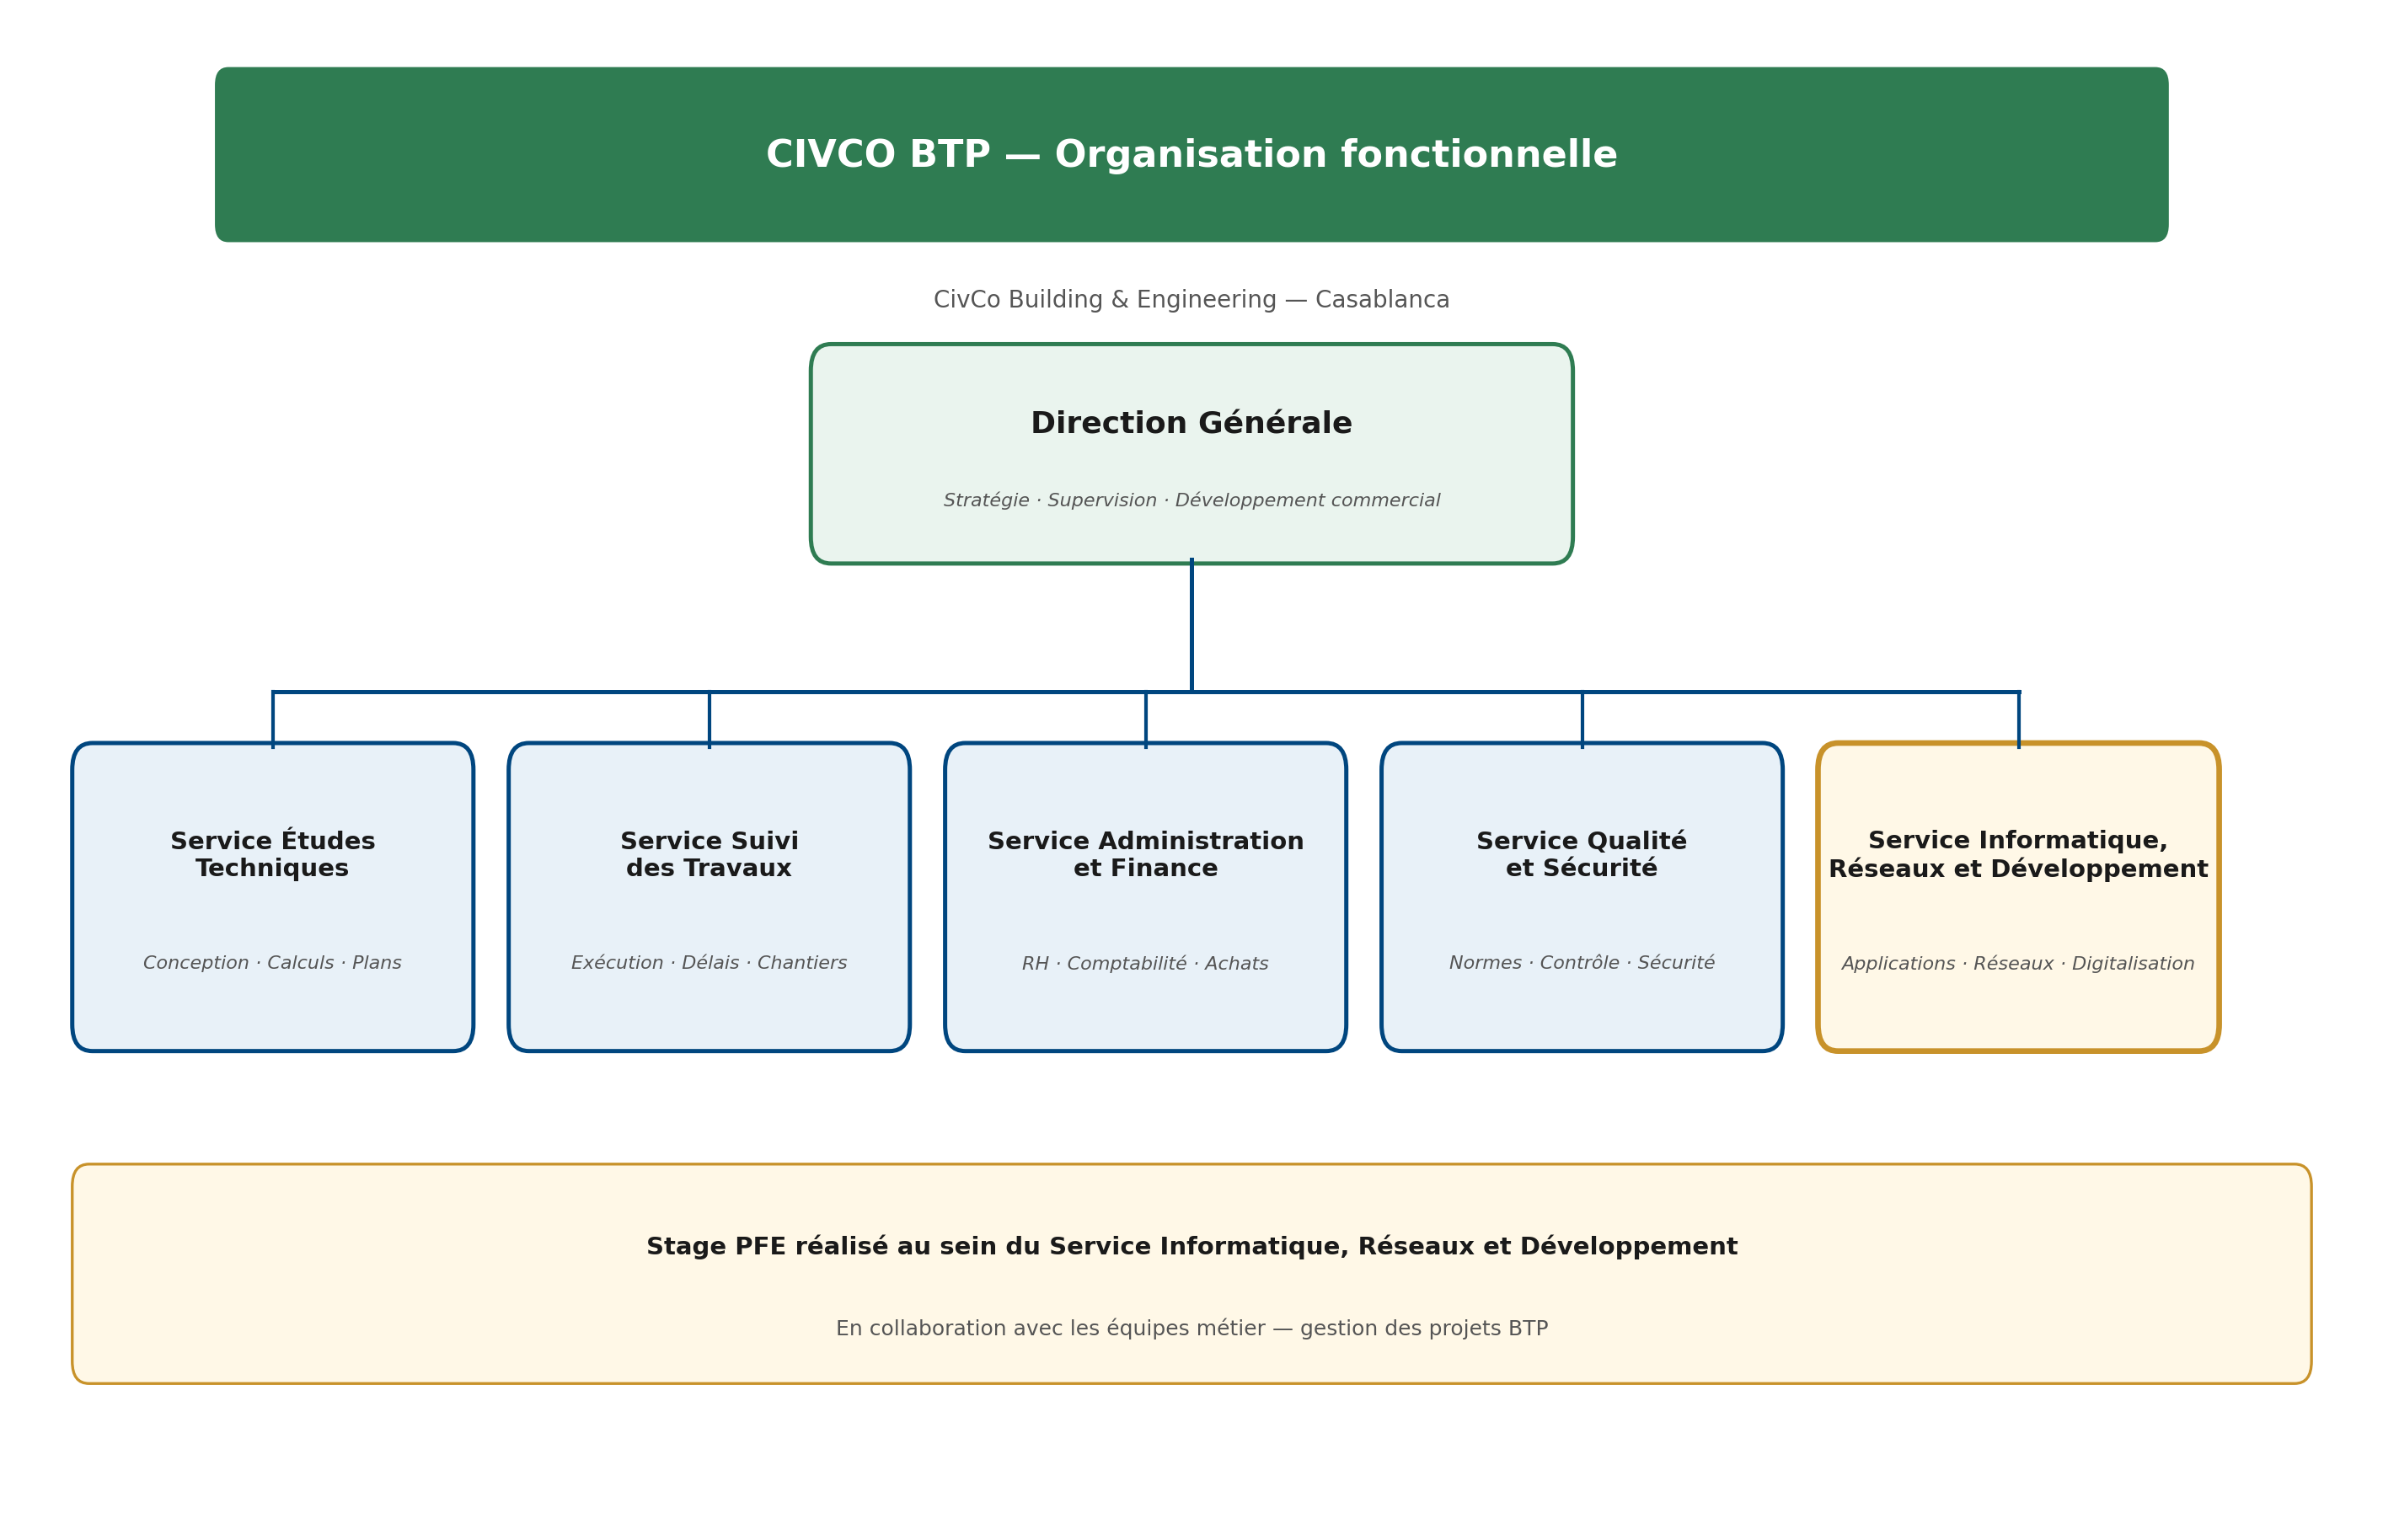
\includegraphics[width=0.85\textwidth]{departments.png}
  \caption{Organisation fonctionnelle de CIVCO BTP}
  \label{fig:civco_org}
\end{figure}

Ce stage s'est déroulé au sein du \textbf{Service Informatique, Réseaux et Développement},
en étroite collaboration avec les équipes métier concernées par la gestion des projets.

\subsection{Domaines d'activité}

Les activités de CIVCO BTP couvrent plusieurs domaines complémentaires :

\medskip

\textbf{Génie civil et études de structures.} Études de bâtiments résidentiels et
industriels, ouvrages publics et infrastructures ; calcul en béton armé, structures
métalliques, dimensionnement des fondations et vérification de stabilité.

\medskip

\textbf{Assistance technique et conseil.} Assistance à maîtrise d'ouvrage, contrôle des
travaux, coordination des intervenants, réception des ouvrages, expertise technique,
études de faisabilité et optimisation des solutions constructives.

\medskip

\textbf{Informatique et développement.} Développement d'applications web et de logiciels
métiers, conception et administration de bases de données, maintenance applicative,
sécurisation des systèmes d'information et déploiement de solutions numériques au service
de la productivité et du suivi des projets.

\medskip

\textbf{Exemples de projets réalisés.} CIVCO BTP intervient sur des chantiers de natures
variées, illustrant la diversité de son portefeuille :

\begin{itemize}
  \item \textbf{Bâtiments résidentiels} : immeubles collectifs, villas haut standing,
  lotissements avec voirie et réseaux.
  \item \textbf{Ouvrages industriels} : halls de production, entrepôts logistiques,
  extensions d'usines existantes.
  \item \textbf{Infrastructures publiques} : voiries urbaines, ouvrages d'assainissement,
  aménagements d'espaces publics.
  \item \textbf{Rénovation et réhabilitation} : mise aux normes parasismiques, extension
  de bâtiments patrimoniaux, restructuration de locaux tertiaires.
\end{itemize}

Cette diversité impose à l'entreprise une capacité d'adaptation et un suivi rigoureux
de chaque affaire, renforçant le besoin d'un outil de gestion centralisé.

\subsection{Moyens humains et matériels}

\textbf{Moyens humains.} L'entreprise s'appuie sur une équipe pluridisciplinaire :
direction générale, ingénieurs génie civil et structures, dessinateurs-projeteurs,
conducteurs de travaux, techniciens, développeurs informatiques, administrateurs réseaux
et systèmes, personnel administratif et financier. Cette diversité de compétences permet
de répondre aux exigences techniques et organisationnelles des projets confiés à CIVCO BTP.

\medskip

\textbf{Moyens matériels.} Sur le plan technique, l'entreprise dispose d'un parc
informatique (postes de travail, serveurs, équipements réseau), de logiciels de conception
(AutoCAD, Revit, Robot Structural Analysis), d'outils de développement (Visual Studio Code,
Git, GitHub) et de systèmes de gestion de bases de données (MySQL, PostgreSQL, SQL Server).
Des véhicules de chantier, une connectivité haut débit et des plateformes collaboratives
complètent l'environnement de travail.

\section{Analyse de l'existant}

Avant de définir la solution cible, une phase d'observation et d'entretiens a été
menée auprès des différents services de CIVCO BTP. L'objectif était de comprendre
comment l'information circule aujourd'hui, quels sont les points de friction et
quels gains une application intégrée pourrait apporter.

\subsection{Processus métier actuels}

Le cycle de vie d'un projet de construction chez CIVCO BTP peut se décomposer en
plusieurs étapes successives, impliquant des acteurs distincts :

\begin{enumerate}
  \item \textbf{Prospection et relation client} : identification du besoin, échanges
  préliminaires, constitution de la fiche client (coordonnées, contacts, historique).
  \item \textbf{Étude et chiffrage} : analyse technique, estimation des coûts,
  production d'un devis détaillé avec lignes de prestations.
  \item \textbf{Contractualisation} : rédaction du contrat, éventuels avenants en cas
  de modification du périmètre ou du budget.
  \item \textbf{Planification} : découpage en phases, affectation de l'équipe,
  définition des tâches opérationnelles et des jalons.
  \item \textbf{Exécution} : suivi de chantier, mise à jour de l'avancement,
  production des bons de livraison et des documents de suivi.
  \item \textbf{Facturation et clôture} : émission des factures, suivi des paiements,
  archivage du dossier projet.
\end{enumerate}

Chaque étape génère des documents et des données qui doivent être partagés entre
le service commercial, les ingénieurs, les conducteurs de travaux, la comptabilité
et parfois le client final. Aujourd'hui, cette circulation repose en grande partie
sur des échanges manuels.

\subsection{Cartographie des outils utilisés}

Le Tableau~\ref{tab:outils_existants} synthétise les outils actuellement mobilisés
par service et leurs limites respectives.

\begin{table}[H]
\caption{Outils actuels et limites identifiées}
\label{tab:outils_existants}
\centering
\small
\begin{tabular}{|l|p{4.2cm}|p{5.8cm}|}
\hline
\textbf{Service} & \textbf{Outils} & \textbf{Limites observées} \\
\hline
Commercial & Excel, Word, courriel & Devis non centralisés, ressaisies \\
\hline
Études / Projets & AutoCAD, Revit, fichiers partagés & Pas de lien avec le suivi financier \\
\hline
Chantier & WhatsApp, tableurs & Informations éphémères, peu traçables \\
\hline
Comptabilité & Logiciel comptable, PDF & Saisie manuelle des factures \\
\hline
Direction & Rapports ponctuels & Absence de tableau de bord temps réel \\
\hline
\end{tabular}
\end{table}

Cette cartographie a confirmé l'absence d'un \textbf{référentiel unique} reliant
clients, projets, documents et équipes. Chaque service dispose de sa propre
organisation documentaire, ce qui complique la consolidation des indicateurs et
la reprise d'information lors d'un changement d'interlocuteur.

\subsection{Besoins exprimés par les services}

Les entretiens menés avec l'encadrant professionnel et les responsables de service
ont permis de formaliser les attentes prioritaires :

\begin{itemize}
  \item \textbf{Direction} : vision consolidée de l'activité (projets actifs,
  retards, charge des équipes).
  \item \textbf{Commercial} : création rapide de devis, historique client,
  conversion simplifiée en facture.
  \item \textbf{Ingénieurs / chefs de projet} : suivi des phases, des tâches et
  de l'équipe affectée à chaque chantier.
  \item \textbf{Comptabilité} : accès aux factures, suivi des paiements et état
  de facturation par projet.
  \item \textbf{Clients} : consultation de l'avancement et validation des
  documents sans dépendre des échanges par courriel.
\end{itemize}

Ces besoins ont orienté le périmètre fonctionnel de l'application développée.

\section{Contexte et problématique}

\subsection{Constats et limites des pratiques actuelles}

Au quotidien, la gestion des projets de construction chez CIVCO BTP mobilise plusieurs
services : études techniques, suivi de travaux, administration, finance et qualité.
Chaque chantier génère un volume important d'informations --- clients, phases, tâches,
devis, factures, contrats, bons de livraison --- qui doivent être partagées entre les
intervenants.

Or, une partie de ces processus repose encore sur des outils non intégrés : fichiers
Excel, documents Word ou PDF isolés, échanges par courriel ou messagerie instantanée.
Cette dispersion entraîne plusieurs difficultés :

\begin{itemize}
  \item \textbf{Fragmentation de l'information} : les données d'un même projet sont
  éparpillées entre plusieurs fichiers et supports.
  \item \textbf{Manque de visibilité} : difficulté à disposer d'une vue d'ensemble sur
  l'avancement des chantiers et des tâches en cours.
  \item \textbf{Risque d'erreurs} : ressaisies manuelles, versions multiples de documents
  et absence de source unique de vérité.
  \item \textbf{Lenteur de coordination} : dépendance aux échanges informels entre
  services pour obtenir une information à jour.
\end{itemize}

\subsection{Problématique}

Face à l'augmentation du nombre de projets et à la complexité croissante de leur suivi,
CIVCO BTP a identifié le besoin de disposer d'un \textbf{outil numérique centralisé} dédié
à la gestion et à la planification de ses projets de construction.

\medskip

La problématique de ce projet peut se formuler ainsi :

\begin{quote}
\textit{Comment concevoir et développer une application web permettant à CIVCO BTP de
centraliser, structurer et piloter l'ensemble du cycle de vie de ses projets de
construction, tout en s'adaptant aux différents profils métier de l'entreprise ?}
\end{quote}

\section{Périmètre du projet}

\subsection{Fonctionnalités incluses}

Le périmètre retenu pour ce stage couvre les modules suivants, considérés comme
prioritaires pour une première version exploitable en interne :

\begin{itemize}
  \item Authentification sécurisée et gestion des rôles (\textbf{RBAC}).
  \item Gestion des projets (phases, équipe, avancement, géolocalisation).
  \item Gestion des clients et provisionnement du portail externe.
  \item Production des documents commerciaux (devis, factures, bons de livraison).
  \item Suivi contractuel (contrats, avenants, modèles de documents).
  \item Planification et suivi des tâches opérationnelles.
  \item Tableau de bord, carte des chantiers et historique des actions.
  \item Messagerie projet entre équipe interne et client.
\end{itemize}

\subsection{Limites et hors périmètre}

Certains sujets ont été volontairement exclus ou reportés à une phase ultérieure,
afin de concentrer l'effort de développement sur le cœur métier :

\begin{itemize}
  \item \textbf{Comptabilité générale} : l'application gère les factures et
  paiements projet, mais ne remplace pas le logiciel comptable de l'entreprise.
  \item \textbf{CAO / BIM} : les outils de conception (AutoCAD, Revit) restent
  indépendants ; seules les métadonnées projet sont centralisées.
  \item \textbf{Gestion des stocks} : non couverte dans cette version.
  \item \textbf{Application mobile native} : l'interface responsive web est
  privilégiée ; une application dédiée est envisagée en perspective.
  \item \textbf{Interopérabilité ERP tiers} : pas d'intégration avec des solutions
  externes (SAP, Sage, etc.) dans le cadre de ce stage.
\end{itemize}

Cette délimitation garantit un livrable cohérent et testable dans la durée du stage,
tout en laissant une base évolutive pour les extensions futures.

\section{Objectifs du projet}

\subsection{Objectif général}

Concevoir et développer une \textbf{application web} de gestion et de planification des
projets de construction pour CIVCO BTP, capable de couvrir les principaux processus métier
liés au suivi des chantiers et à la production des documents commerciaux.

\subsection{Objectifs fonctionnels}

\begin{itemize}
  \item \textbf{Gestion des projets} : créer, consulter et suivre les chantiers par phases,
  avec affectation des équipes et suivi de l'avancement.
  \item \textbf{Gestion des clients} : centraliser les informations clients, contacts et
  historique des projets associés.
  \item \textbf{Documents commerciaux} : produire et suivre les devis, factures et bons de
  livraison (\textbf{BL}) liés aux projets.
  \item \textbf{Suivi contractuel} : gérer les contrats et les avenants associés aux
  chantiers.
  \item \textbf{Planification des tâches} : organiser le travail opérationnel par phases
  et attribuer les tâches aux collaborateurs.
  \item \textbf{Tableau de bord} : offrir une vue synthétique de l'activité (projets en
  cours, indicateurs clés, tâches prioritaires).
  \item \textbf{Contrôle d'accès} : garantir que chaque utilisateur accède uniquement aux
  fonctionnalités correspondant à son rôle (\textbf{RBAC}).
\end{itemize}

\subsection{Objectifs techniques}

\begin{itemize}
  \item Mettre en place une architecture \textit{full-stack} avec un \textit{backend} API
  \textbf{Laravel} / \textbf{PHP} et une interface \textbf{React} en \textbf{SPA}.
  \item Concevoir une base de données relationnelle (\textbf{SQL}) modélisant les entités
  métier (projets, clients, documents, utilisateurs, rôles).
  \item Exposer des services \textbf{REST} sécurisés pour la communication entre le
  \textit{frontend} et le \textit{backend}.
  \item Assurer une interface ergonomique, responsive et adaptée à un usage professionnel
  quotidien.
  \item Valider le bon fonctionnement des modules développés par des tests manuels et,
  le cas échéant, des tests automatisés.
\end{itemize}

\section{Méthodologie adoptée}

\subsection{Démarche de développement}

Le projet a été mené selon une approche \textbf{itérative et incrémentale}, adaptée au
contexte d'un stage en entreprise. Le travail s'est déroulé en plusieurs étapes :

\begin{enumerate}
  \item \textbf{Analyse des besoins} : recueil des attentes auprès de l'encadrant
  professionnel et identification des modules prioritaires.
  \item \textbf{Conception} : modélisation des entités métier, définition de l'architecture
  technique et des cas d'utilisation principaux.
  \item \textbf{Développement par modules} : implémentation progressive des fonctionnalités
  (projets, clients, documents commerciaux, tâches, tableau de bord, etc.).
  \item \textbf{Tests et validation} : vérification du comportement de chaque module et
  correction des anomalies identifiées.
  \item \textbf{Documentation} : rédaction du présent rapport et documentation technique
  du code produit.
\end{enumerate}

Chaque itération visait à livrer un incrément fonctionnel, démontrable lors des réunions
de suivi, avant de passer au module suivant.

\subsection{Gestion de projet avec Trello}

Le suivi opérationnel du stage a été organisé à l'aide de \textbf{Trello}, outil de
gestion de projet en ligne basé sur la méthode \textbf{Kanban}. Un tableau dédié au
projet regroupait les tâches sous forme de cartes réparties en colonnes selon leur
état : \textit{À faire}, \textit{En cours}, \textit{En revue} et \textit{Terminé}.

\medskip

Chaque carte correspondait à une fonctionnalité, une correction ou une tâche de
conception (par exemple : « Module devis --- API backend », « Écran tableau de bord »,
« Tests RoleAccess »). Les cartes précisaient une brève description, une priorité et,
le cas échéant, une échéance. Cette organisation a permis de :

\begin{itemize}
  \item visualiser l'avancement global du projet en un coup d'œil ;
  \item prioriser les modules à développer en accord avec l'encadrant professionnel ;
  \item conserver une trace des tâches réalisées et de celles restant à traiter ;
  \item préparer les démonstrations lors des réunions de suivi hebdomadaires.
\end{itemize}

Trello a ainsi complété Git/GitHub : le premier pour la planification et le suivi
des livrables métier, le second pour le versionnement du code source.

\subsection{Suivi académique et professionnel}

\textbf{Suivi académique (EMSI Casablanca) :}
\begin{itemize}
  \item Encadrant pédagogique : \textbf{Pr. Mohammed El Assad}
  \item Réunions régulières de suivi, validation de la démarche et préparation de la
  soutenance finale.
\end{itemize}

\textbf{Suivi professionnel (CIVCO BTP) :}
\begin{itemize}
  \item Encadrant professionnel : \textbf{M. Mohamed BENABDELLAH-CHAOUNI}
  \item Réunions de suivi pour présenter l'avancement, valider les choix fonctionnels et
  recueillir les retours métier.
  \item Alignement continu du développement avec les besoins réels de l'entreprise.
\end{itemize}

\subsection{Outils et environnement de travail}

\textbf{Outils de développement :}
\begin{itemize}
  \item \textbf{Trello} : gestion de projet et suivi des tâches (tableau Kanban).
  \item \textbf{Git / GitHub} : gestion de versions et suivi des évolutions du code.
  \item \textbf{Visual Studio Code} : environnement de développement principal.
  \item \textbf{Laravel} : framework \textit{backend} (\textbf{MVC}, \textbf{ORM} Eloquent).
  \item \textbf{React + Vite} : interface utilisateur (\textbf{SPA}).
  \item \textbf{MySQL / PostgreSQL} : base de données relationnelle.
\end{itemize}

\textbf{Environnements :}
\begin{itemize}
  \item \textbf{Développement} : poste local avec serveur Laravel et serveur de
  développement Vite (\textit{hot-reload}).
  \item \textbf{Tests} : validation manuelle des parcours utilisateurs et tests
  fonctionnels sur les modules livrés.
\end{itemize}

\section{Planification du stage}

Le stage s'est déroulé sur la période \textbf{avril -- juillet 2026}, au sein du service
informatique de CIVCO BTP. La planification générale du projet peut se résumer comme suit :

\begin{table}[H]
\centering
\caption{Phases principales du projet de stage}
\label{tab:planification}
\begin{tabularx}{\textwidth}{|l|X|}
\hline
\textbf{Phase} & \textbf{Activités principales} \\
\hline
Analyse & Étude de l'existant, recueil des besoins, définition du périmètre \\
\hline
Conception & Modélisation UML, architecture technique, maquettage des interfaces \\
\hline
Développement & Implémentation progressive des modules (\textit{backend} et \textit{frontend}) \\
\hline
Tests & Vérification fonctionnelle, corrections et stabilisation \\
\hline
Rédaction & Rédaction du rapport de fin d'études et préparation de la soutenance \\
\hline
\end{tabularx}
\end{table}

\subsection{Planning détaillé par période}

Le Tableau~\ref{tab:planning_detail} détaille la répartition des activités sur
les quatre mois du stage. Chaque période correspond à un jalon de démonstration
validé avec l'encadrant professionnel.

\begin{table}[H]
\centering
\caption{Planning détaillé du stage (avril -- juillet 2026)}
\label{tab:planning_detail}
\small
\begin{tabularx}{\textwidth}{|l|X|}
\hline
\textbf{Période} & \textbf{Livrables et activités} \\
\hline
Avril 2026 &
Analyse de l'existant, entretiens métier, rédaction du cahier des charges fonctionnel,
validation du périmètre avec l'encadrant professionnel \\
\hline
Mai 2026 &
Conception UML (cas d'utilisation, séquence, classes), modélisation de la base de données,
architecture technique three-tier, maquettage des écrans principaux \\
\hline
Juin 2026 &
Développement backend Laravel (authentification, projets, clients, devis, factures),
mise en place du frontend React (navigation, tableau de bord), premières démonstrations
des modules livrés \\
\hline
Juillet 2026 &
Portail client, tâches, configuration des rôles, tests PHPUnit et validation manuelle,
stabilisation, rédaction du rapport de fin d'études et préparation de la soutenance \\
\hline
\end{tabularx}
\end{table}

\medskip

Cette planification incrémentale a permis de livrer des modules testables au fur
et à mesure, tout en ajustant les priorités en fonction des retours terrain.
Par exemple, le module d'impression documentaire et le suivi des copies officielles
ont été intégrés en cours de développement suite à une demande exprimée par la
direction administrative.

\newpage
\section*{Conclusion}

Ce chapitre a posé le cadre du projet de fin d'études réalisé au sein de
\textbf{CIVCO BTP}. Nous avons présenté l'organisme d'accueil, son organisation
et les domaines d'activité du bureau d'études, afin de situer le projet dans son
contexte métier BTP. L'analyse de l'existant a mis en évidence la dispersion des
outils (tableurs, documents isolés, échanges informels) et la difficulté à disposer
d'une vision consolidée des chantiers, des clients et des documents commerciaux.

\medskip

À partir de cette problématique, nous avons formulé les objectifs fonctionnels et
techniques de l'application : centraliser la gestion des projets, des clients, des
devis, des factures et du suivi opérationnel, tout en garantissant un contrôle
d'accès par rôles adapté aux différents profils de l'entreprise. Le périmètre retenu
couvre les modules prioritaires identifiés avec l'encadrant professionnel, dans une
logique de livrable progressif et testable.

\medskip

La méthodologie adoptée combine une approche \textbf{agile incrémentale}, un suivi
\textbf{Kanban} via \textbf{Trello} et un versionnement \textbf{Git/GitHub}.
Le planning sur quatre mois (avril -- juillet 2026) a structuré les phases d'analyse,
de conception, de développement et de validation, avec des jalons de démonstration
réguliers. Ce cadrage constitue la base sur laquelle s'appuient les chapitres
suivants.

\medskip

Le chapitre suivant expose l'état de l'art des technologies mobilisées et justifie
les choix techniques retenus --- architecture \textit{full-stack}, \textbf{Laravel},
\textbf{React} et base de données relationnelle --- pour la réalisation de
l'application.

\chapter{État de l'Art et Étude Théorique}
\label{chap:etat_art}

\section{Introduction}

L'application développée pour CIVCO BTP s'appuie sur un ensemble de technologies web
modernes, réparties entre un \textit{backend} API, une base de données relationnelle et
une interface utilisateur riche. Ce chapitre constitue le socle théorique du rapport :
il présente les concepts et les technologies étudiés, puis justifie les choix retenus
pour la réalisation du projet.

\medskip

Nous abordons successivement les \textbf{architectures des applications web}, le
\textbf{framework Laravel} côté serveur, les \textbf{interfaces React en SPA}, les
\textbf{bases de données relationnelles et l'ORM}, les \textbf{API REST et
l'authentification}, ainsi que les \textbf{solutions ERP et outils de gestion de projets
dans le secteur du BTP}. Le chapitre se conclut par une référence comparative
(\textit{benchmark}) justifiant chaque choix technologique retenu.

% ─────────────────────────────────────────────────────────────────────
\section{Les applications web et l'architecture full-stack}
\subsection{Évolution des applications web}

Les applications de gestion d'entreprise ont connu une évolution majeure au cours des
deux dernières décennies. Les premières solutions reposaient sur des architectures
\textbf{monolithiques} : logique métier, interface et base de données regroupées dans
un même programme, souvent accessible via un navigateur avec rechargement complet de
page à chaque action.

\medskip

L'émergence des \textbf{API} (\textit{Application Programming Interface}) a séparé la
couche de présentation de la couche métier. Le navigateur ou une application mobile
consomme des services distants via \textbf{HTTP}, échangeant des données structurées en
\textbf{JSON}. Cette découpe a ouvert la voie aux architectures \textit{full-stack}
modernes, dans lesquelles un \textit{frontend} JavaScript riche dialogue avec un
\textit{backend} API indépendant~\cite{fielding2000rest}.

\subsection{Architecture client-serveur et tiers}

L'architecture \textbf{three-tier} (\textit{trois tiers}) structure l'application en
trois couches distinctes :

\begin{enumerate}
  \item \textbf{Couche présentation} : interface utilisateur (React), exécutée dans le
  navigateur.
  \item \textbf{Couche métier} : logique applicative, règles de gestion, authentification
  (Laravel).
  \item \textbf{Couche données} : persistance relationnelle (MySQL / PostgreSQL).
\end{enumerate}

Cette séparation améliore la maintenabilité : chaque couche peut évoluer indépendamment
tant que les contrats d'interface (API REST) sont respectés. Fowler~\cite{fowler2019patterns}
décrit ce découpage comme un patron fondamental des applications d'entreprise.

\begin{figure}[H]
  \centering
  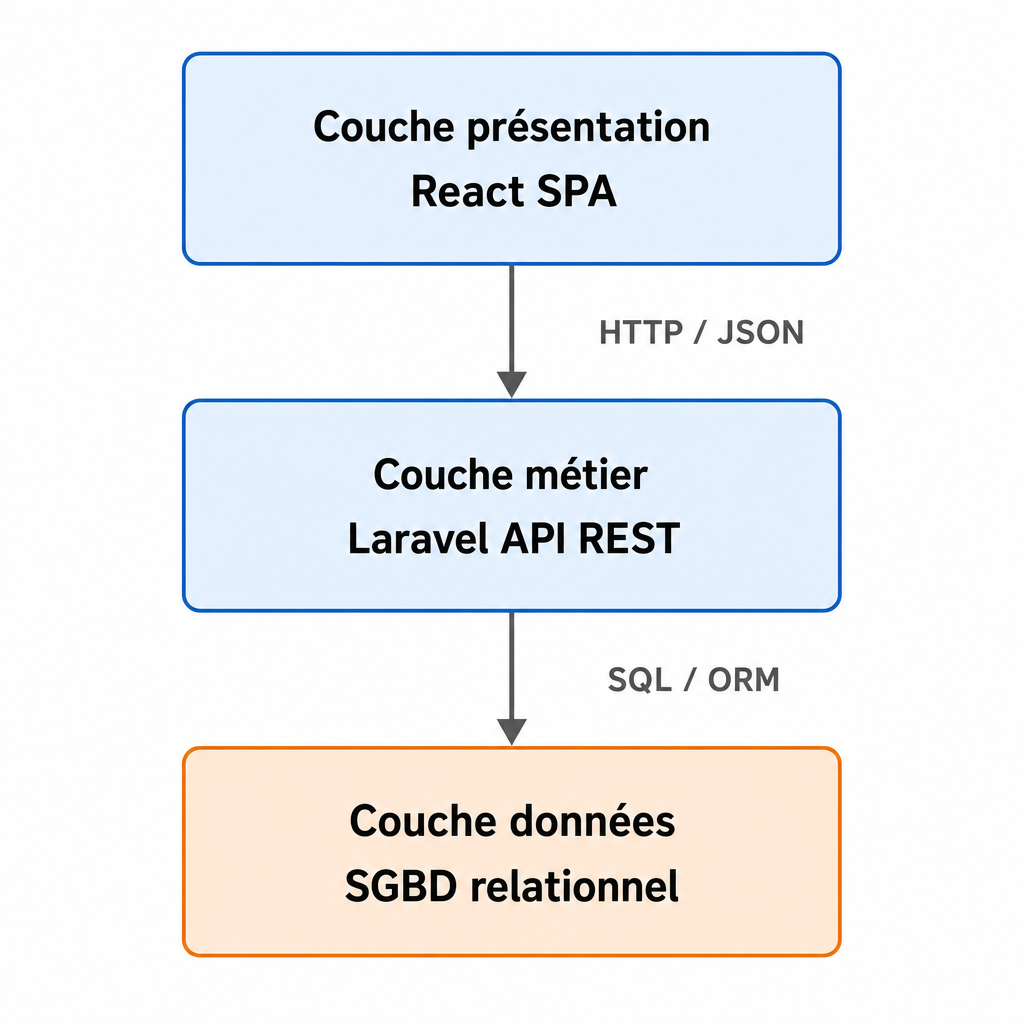
\includegraphics[width=0.55\textwidth]{fig_2_1_three_tier_preview.png}
  \caption{Architecture three-tier de l'application CIVCO BTP}
  \label{fig:three_tier}
\end{figure}

\subsection{Single Page Application (SPA)}

Une \textbf{SPA} (\textit{Single Page Application}) charge une seule page HTML, puis
met à jour dynamiquement le contenu via JavaScript sans rechargement complet. Les
avantages pour une application métier sont significatifs :

\begin{itemize}
  \item \textbf{Fluidité} : navigation instantanée entre les modules (projets, clients,
  factures).
  \item \textbf{Expérience utilisateur} : interfaces réactives, proches des applications
  de bureau.
  \item \textbf{Réutilisation de l'état} : conservation du contexte utilisateur
  (filtres, session) entre les écrans.
\end{itemize}

Le couplage d'une SPA React avec une API Laravel constitue aujourd'hui un standard
industriel pour les tableaux de bord et outils de gestion internes.

\subsection{Panorama des stacks full-stack}

\begin{table}[H]
\caption{Panorama des stacks full-stack pour applications métier}
\label{tab:stack_panorama}
\centering
\small
\begin{tabular}{|l|l|p{8cm}|}
\hline
\textbf{Stack} & \textbf{Langages} & \textbf{Caractéristiques} \\
\hline
LAMP / LEMP & PHP + MySQL & Mature, hébergement abordable, Laravel/Symfony \\
\hline
MERN / MEAN & JavaScript & Un seul langage, Node.js + MongoDB \\
\hline
Django + React & Python + JS & Rapidité backend, ORM Django \\
\hline
\textbf{Laravel + React} & PHP + JS & API REST + SPA, écosystème riche \\
\hline
.NET + Angular & C\# + TS & Écosystème Microsoft, entreprise \\
\hline
\end{tabular}
\end{table}

Pour CIVCO BTP, la stack \textbf{Laravel + React} (Tableau~\ref{tab:stack_panorama})
offre le meilleur compromis entre productivité, courbe d'apprentissage et adéquation
avec les compétences visées en filière IIR : développement web, bases de données et
architecture logicielle.

\subsection{Échange de données et format JSON}

Les API modernes échangent des données structurées en \textbf{JSON} (\textit{JavaScript
Object Notation}), format léger et lisible, natif en JavaScript et bien supporté par
PHP/Laravel. Chaque ressource métier est sérialisée en objet JSON : un projet expose
son identifiant, son client associé, ses phases, son statut et ses dates ; un devis
expose ses lignes, montants et statut de validation.

\medskip

Ce format facilite le découplage frontend/backend : React consomme directement les
réponses JSON, les mappe vers ses composants et met à jour l'interface sans
transformation complexe. Les codes de statut HTTP (\texttt{200}, \texttt{201},
\texttt{422}, \texttt{403}) signalent le résultat de chaque opération de façon
standardisée.

\subsection{Patterns CRUD et ressources métier}

La majorité des modules de l'application suivent le pattern \textbf{CRUD}
(\textit{Create, Read, Update, Delete}) : créer un client, lister les projets,
modifier une facture, archiver un document. Laravel formalise ce pattern via les
contrôleurs de ressources et les routes RESTful, ce qui garantit une cohérence
d'API sur l'ensemble des modules (clients, projets, devis, factures, tâches,
contrats).


% ─────────────────────────────────────────────────────────────────────
\section{Le framework Laravel et l'écosystème PHP}
\subsection{Présentation de PHP et Laravel}

\textbf{PHP} est un langage de script côté serveur largement déployé sur le web.
Historiquement associé au développement de sites dynamiques, il a évolué vers des
versions modernes (8.x) intégrant un typage strict, des performances accrues (JIT) et
un écosystème mature de frameworks.

\medskip

\textbf{Laravel}~\cite{laravel} est le framework PHP le plus adopté pour construire des
applications web et des API. Créé par Taylor Otwell, il impose une structure claire
autour du patron \textbf{MVC} (\textit{Model-View-Controller}) et propose des
composants intégrés pour les tâches courantes : routage, validation, authentification,
files d'attente, envoi de courriels et gestion des fichiers.

\subsection{Architecture MVC dans Laravel}

Le patron \textbf{MVC} répartit les responsabilités :

\begin{itemize}
  \item \textbf{Modèle} : représentation des entités métier et accès aux données
  (Eloquent).
  \item \textbf{Vue} : dans une API, les \textit{Resources} et \textit{Collections}
  formatent les réponses JSON pour le client.
  \item \textbf{Contrôleur} : reçoit la requête HTTP, applique la validation, invoque
  les services métier et retourne la réponse.
\end{itemize}

Cette organisation facilite la lecture du code et l'ajout de nouveaux modules. Pour
l'application CIVCO BTP, chaque domaine métier (projets, clients, devis, factures)
dispose de son contrôleur, de ses modèles et de ses règles de validation.

\subsection{Composants clés de l'écosystème Laravel}

\subsubsection{Routage et validation}

Le fichier de routes (\texttt{routes/api.php}) déclare les points d'entrée de l'API.
Chaque route est associée à un contrôleur et protégée par des \textit{middleware}
(vérification d'authentification, contrôle de permissions, contexte entreprise).

Les \textbf{Form Requests} encapsulent les règles de validation des données entrantes
(ex.~: champs obligatoires d'un devis, formats de dates, montants positifs), garantissant
l'intégrité des données avant persistance.

\subsubsection{Services et logique métier}

Au-delà des contrôleurs, la logique complexe est extraite dans des classes
\textbf{Service} (\texttt{QuoteService}, \texttt{PrintTrackingService}, etc.). Ce
découpage respecte le principe de responsabilité unique : le contrôleur orchestre,
le service implémente la règle métier.

\subsubsection{Migrations et seeders}

Les \textbf{migrations} versionnent le schéma de la base de données sous forme de fichiers
PHP exécutables de façon reproductible. Les \textbf{seeders} initialisent des données
de référence (rôles, permissions, données de démonstration), indispensables pour
tester l'application en conditions proches du réel.

\subsection{Comparaison avec les alternatives PHP}

\begin{table}[H]
\caption{Comparaison des frameworks PHP pour une API REST}
\label{tab:php_frameworks}
\centering
\small
\begin{tabular}{|l|p{4cm}|p{4cm}|p{4cm}|}
\hline
\textbf{Framework} & \textbf{Philosophie} & \textbf{Forces} & \textbf{Contexte idéal} \\
\hline
\textbf{Laravel} & Convention over configuration & Écosystème complet, Sanctum, Eloquent &
API + SPA, PME/ETI \\
\hline
Symfony & Composants réutilisables & Modularité, robustesse & Grandes applications \\
\hline
CodeIgniter & Minimaliste & Légèreté & Petits projets \\
\hline
\end{tabular}
\end{table}

Laravel ressort du Tableau~\ref{tab:php_frameworks} pour un projet de gestion métier
nécessitant authentification, RBAC, documents et évolutivité --- le profil exact du
projet CIVCO BTP.

\subsection{Laravel dans le projet CIVCO BTP}

L'API Laravel expose plus de quarante contrôleurs organisés par domaine, des
\textit{middleware} de contrôle d'accès et un ensemble de services métier. Cette
structure permet d'ajouter progressivement de nouveaux modules (avenants contractuels,
modèles de documents, suivi d'impression) sans remettre en cause l'architecture
existante.

\subsection{Middleware, Resources et couche de présentation API}

\subsubsection{Middleware}

Les \textbf{middleware} Laravel interceptent chaque requête HTTP avant qu'elle
n'atteigne le contrôleur. Dans le projet, plusieurs middlewares assurent la
sécurité et le contexte métier :

\begin{itemize}
  \item \textbf{Authentification Sanctum} : vérifie que l'utilisateur est connecté.
  \item \textbf{Contrôle de permissions} : valide que l'utilisateur possède la
  permission requise (\texttt{project.view}, \texttt{quote.manage}, etc.).
  \item \textbf{Contexte entreprise} : identifie la société courante via l'en-tête
  \texttt{X-Company-Id}, garantissant l'isolation des données métier.
\end{itemize}

\subsubsection{API Resources}

Les classes \textbf{Resource} (\texttt{ProjectResource}, \texttt{InvoiceResource},
etc.) transforment les modèles Eloquent en tableaux JSON normalisés. Elles permettent
de contrôler précisément les champs exposés à l'interface, d'inclure conditionnellement
des relations (\texttt{client}, \texttt{lines}, \texttt{teamMembers}) et d'uniformiser
le format de réponse sur toute l'API.

\subsubsection{Validation et gestion des erreurs}

Lorsqu'une requête échoue la validation, Laravel retourne une réponse \texttt{422}
avec le détail des champs en erreur. Le frontend React intercepte ces réponses pour
afficher des messages à l'utilisateur, améliorant l'expérience de saisie sur les
formulaires de devis, factures et fiches projets.


% ─────────────────────────────────────────────────────────────────────
\section{React et les Single Page Applications}
\subsection{Définition et principes des SPA}

Une \textbf{SPA} (\textit{Single Page Application}) est une application web dont
l'interface est construite dynamiquement en JavaScript. Contrairement aux sites
classiques où chaque clic déclenche un rechargement HTML complet, la SPA charge le
shell de l'application une fois, puis met à jour le DOM (\textit{Document Object Model})
au fil des interactions utilisateur.

\medskip

Ce modèle repose sur le \textbf{routing côté client} : la bibliothèque React Router
associe chaque URL à un composant React (\texttt{/projects}, \texttt{/clients},
\texttt{/invoices}), sans solliciter le serveur pour le HTML. Seules les données
nécessaires sont récupérées via l'API REST.

\subsection{React : bibliothèque declarative}

\textbf{React}~\cite{react}, développé par Meta, est une bibliothèque JavaScript pour
construire des interfaces utilisateur par \textbf{composants} réutilisables. Chaque
composant encapsule structure (JSX), état et comportement.

\medskip

Les principes fondamentaux de React sont :

\begin{itemize}
  \item \textbf{Composants fonctionnels} : fonctions JavaScript retournant du JSX,
  composées hiérarchiquement (Sidebar, Dashboard, ProjectDetailPage, etc.).
  \item \textbf{État local} (\texttt{useState}) : données modifiables au sein d'un
  composant (formulaires, filtres, modales).
  \item \textbf{Effets de bord} (\texttt{useEffect}) : chargement de données API au
  montage du composant ou lors d'un changement de paramètre.
  \item \textbf{Context API} : partage d'état global (authentification, thème, langue)
  sans propager les props à travers toute l'arborescence.
\end{itemize}

Cette approche declarative simplifie la construction d'interfaces complexes : l'état
de l'interface est une fonction de l'état applicatif.

\subsection{Écosystème React du projet}

L'application CIVCO BTP s'appuie sur plusieurs bibliothèques complémentaires :

\begin{table}[H]
\caption{Composants de l'écosystème frontend}
\label{tab:react_ecosystem}
\centering
\small
\begin{tabular}{|l|l|p{7.5cm}|}
\hline
\textbf{Outil} & \textbf{Rôle} & \textbf{Usage dans le projet} \\
\hline
Vite~\cite{vite} & Build tool & Compilation rapide, HMR en développement \\
\hline
React Router & Routing & Navigation entre modules ERP \\
\hline
Axios & Client HTTP & Appels API REST avec intercepteurs \\
\hline
Tailwind CSS~\cite{tailwindcss} & Styles utilitaires & Interface sombre cohérente \\
\hline
Recharts & Graphiques & Tableau de bord, KPIs \\
\hline
Leaflet & Cartographie & Carte des projets / chantiers \\
\hline
\end{tabular}
\end{table}

\subsection{Communication avec le backend}

Le \textit{frontend} React consomme l'API Laravel via des modules dédiés
(\texttt{api/projects.js}, \texttt{api/clients.js}, etc.). Un client Axios centralisé
configure :

\begin{itemize}
  \item l'envoi automatique des cookies de session (Sanctum) ;
  \item le jeton CSRF pour les requêtes \texttt{POST}, \texttt{PUT} et \texttt{DELETE} ;
  \item la gestion des erreurs \texttt{401} (redirection vers la page de connexion).
\end{itemize}

Ce patron \textit{API-first} garantit que toute action utilisateur (créer un devis,
archiver un client, assigner une tâche) transite par la couche métier Laravel, où les
règles de validation et de permissions sont appliquées.

\begin{figure}[H]
\centering
\resizebox{0.92\textwidth}{!}{%
\begin{tikzpicture}[
  box/.style={rectangle, rounded corners=4pt, fill=ensamBlue!12, draw=ensamBlue,
              minimum width=3.2cm, minimum height=1.0cm, align=center,
              font=\small\bfseries},
  arr/.style={-{Stealth[length=6pt]}, thick, draw=gray!70},
  lbl/.style={font=\footnotesize, text=gray!70}
]
  \node[box] (browser) at (0, 0)   {Navigateur\\React SPA};
  \node[box] (api)     at (5.5, 0) {API Laravel\\REST + Sanctum};
  \node[box] (db)      at (11, 0)  {Base de\\données};

  \draw[arr] (browser) -- (api) node[midway, above, lbl] {JSON / HTTPS};
  \draw[arr] (api)     -- (db)  node[midway, above, lbl] {Eloquent / SQL};
\end{tikzpicture}
}%
\caption{Flux de communication React $\rightarrow$ Laravel $\rightarrow$ SGBD}
\label{fig:react_flow}
\end{figure}

\subsection{Comparaison React / Vue / Angular}

\begin{table}[H]
\caption{Comparaison des principaux frameworks frontend (2025-2026)}
\label{tab:spa_compare}
\centering
\small
\begin{tabular}{|l|p{3.5cm}|p{3.5cm}|p{3.5cm}|}
\hline
\textbf{Critère} & \textbf{React} & \textbf{Vue.js} & \textbf{Angular} \\
\hline
Flexibilité & Élevée (bibliothèque) & Élevée (progressif) & Opinionated (framework complet) \\
\hline
Courbe d'apprentissage & Modérée & Faible & Élevée \\
\hline
Marché de l'emploi & Très large & Large & Large (entreprise) \\
\hline
Écosystème SPA & React Router, Vite & Vue Router, Vite & Router intégré \\
\hline
\end{tabular}
\end{table}

React est retenu pour sa flexibilité, son adoption industrielle et la disponibilité de
bibliothèques adaptées aux tableaux de bord métier (graphiques, cartes, composants
modulaires), comme le montre le Tableau~\ref{tab:spa_compare}.

\subsection{Organisation du code frontend}

Le code React est structuré par \textbf{features} (\texttt{features/projects/},
\texttt{features/clients/}, \texttt{features/invoices/}), chacune regroupant pages,
composants et utilitaires propres au module. Les composants transverses (Sidebar,
PermissionGate, modales) vivent dans \texttt{components/}. Cette organisation par
domaine facilite la navigation dans le code et l'ajout de nouvelles fonctionnalités
sans impacter les modules existants.

\subsection{Interface utilisateur et Tailwind CSS}

L'interface adopte un design sombre professionnel, cohérent sur tous les modules.
\textbf{Tailwind CSS}~\cite{tailwindcss} est un framework CSS utilitaire : les classes
(\texttt{flex}, \texttt{rounded-lg}, \texttt{bg-gray-800}) s'appliquent directement
dans le JSX. Cette approche accélère le prototypage et garantit une cohérence visuelle
sur les écrans de l'application (listes, fiches détail, modales, tableaux de bord).

\medskip

Le \textbf{tableau de bord} illustre l'intérêt de React pour la visualisation métier :
graphiques (Recharts), widgets configurables, indicateurs \textbf{KPI} et accès rapide
aux projets en cours. La carte des chantiers (Leaflet) offre une vue géographique des
projets, pertinente pour une entreprise disposant de plusieurs sites simultanés.

\subsection{Internationalisation}

L'application supporte le \textbf{français} (langue par défaut) et l'\textbf{anglais}
via un contexte de langue et des fichiers de traduction (\texttt{locales/fr.js},
\texttt{locales/en.js}). Cette préparation facilite l'usage de l'outil par des
collaborateurs anglophones ou une future extension à d'autres contextes linguistiques.


% ─────────────────────────────────────────────────────────────────────
\section{Les bases de données relationnelles et l'ORM}

\subsection{Modèle relationnel et SGBD}

Une application de gestion de projets manipule des entités fortement structurées et
liées entre elles : clients, projets, phases, tâches, devis, factures, contrats,
utilisateurs et rôles. Le \textbf{modèle relationnel}, formalisé par Codd, organise ces
données en tables reliées par des clés étrangères, garantissant l'intégrité référentielle
et la cohérence des enregistrements~\cite{fowler2019patterns}.

\medskip

Les \textbf{SGBD} (\textit{Systèmes de Gestion de Bases de Données}) relationnels les
plus répandus en environnement web sont \textbf{MySQL}~\cite{mysql} et
\textbf{PostgreSQL}~\cite{postgresql}. MySQL se distingue par sa simplicité de déploiement
et sa large adoption ; PostgreSQL offre des fonctionnalités avancées (contraintes
complexes, types JSON, performances sur de gros volumes). Pour une application métier
comme celle de CIVCO BTP, les deux systèmes conviennent ; le choix final dépend de
l'environnement d'hébergement et des besoins de montée en charge.

\subsection{L'ORM et Eloquent}

Manipuler directement le langage \textbf{SQL} dans chaque composant applicatif alourdit
le code et complique la maintenance. L'\textbf{ORM} (\textit{Object-Relational Mapping})
fait correspondre les tables de la base à des classes du langage de programmation.
Dans Laravel, \textbf{Eloquent} fournit une couche d'abstraction élégante :

\begin{itemize}
  \item chaque table est représentée par un \textbf{modèle} (\texttt{Project},
  \texttt{Client}, \texttt{Invoice}, etc.) ;
  \item les relations (\texttt{hasMany}, \texttt{belongsTo}, \texttt{belongsToMany})
  expriment les liens métier de façon déclarative ;
  \item les migrations versionnent le schéma de la base et facilitent le déploiement
  entre environnements ;
  \item les \textit{seeders} permettent de peupler la base avec des données de démonstration.
\end{itemize}

Cette approche accélère le développement, réduit les erreurs de requêtes et aligne le
code objet sur le modèle métier de l'entreprise.

\subsection{Normalisation et intégrité des données}

La conception d'une base pour un ERP léger repose sur plusieurs principes :

\begin{itemize}
  \item \textbf{Normalisation} : éviter la duplication d'informations (un client est
  enregistré une seule fois, référencé par ses projets et documents).
  \item \textbf{Contraintes d'intégrité} : clés étrangères, unicité des identifiants
  métier (numéros de devis, de facture).
  \item \textbf{Traçabilité} : horodatage des enregistrements (\texttt{created\_at},
  \texttt{updated\_at}) et journalisation des actions sensibles.
\end{itemize}

Ces principes sont essentiels dans un contexte BTP où les documents commerciaux et
contractuels doivent rester cohérents et auditables.

\subsection{Modèle de données métier}

Le schéma relationnel de l'application modélise les entités principales du cycle de
vie d'un projet CIVCO BTP :

\begin{table}[H]
\centering
\small
\caption{Entités principales du modèle de données}
\label{tab:entities}
\begin{tabular}{|l|p{9cm}|}
\hline
\textbf{Entité} & \textbf{Rôle} \\
\hline
Client & Maître d'ouvrage ou client commercial, contacts associés \\
\hline
Project & Chantier / projet, lié à un client, phases et équipe \\
\hline
ProjectPhase & Découpage temporel du projet (études, exécution, réception) \\
\hline
Task & Tâche opérationnelle assignée à un collaborateur \\
\hline
Quote / Invoice & Documents commerciaux avec lignes de détail \\
\hline
Contract & Contrat et avenants liés au projet \\
\hline
User / Role & Utilisateurs internes et permissions RBAC \\
\hline
\end{tabular}
\end{table}

Les relations entre ces entités (un client possède plusieurs projets, un projet
contient plusieurs phases et tâches, un devis peut être converti en facture) sont
implémentées via Eloquent et contraintes de clés étrangères en base.

% ─────────────────────────────────────────────────────────────────────
\section{Les API REST et l'authentification}

\subsection{Principe des API REST}

Une \textbf{API REST} (\textit{Representational State Transfer}) expose des ressources
(identifiées par des URL) manipulables via les verbes \textbf{HTTP} :
\texttt{GET} (lecture), \texttt{POST} (création), \texttt{PUT/PATCH} (mise à jour),
\texttt{DELETE} (suppression)~\cite{fielding2000rest}. Ce style architectural sépare
clairement le \textit{frontend} (interface utilisateur) du \textit{backend} (logique
métier et persistance), ce qui permet :

\begin{itemize}
  \item de faire évoluer l'interface sans réécrire le serveur ;
  \item de réutiliser la même API pour d'éventuels clients mobiles futurs ;
  \item de tester indépendamment chaque couche.
\end{itemize}

Dans le projet CIVCO BTP, l'API est organisée sous le préfixe \texttt{/api/v1/} et
expose des ressources métier : projets, clients, devis, factures, tâches, etc.

\subsection{Authentification et contrôle d'accès}

La sécurisation d'une application métier repose sur deux piliers :

\medskip

\textbf{Authentification.} Laravel \textbf{Sanctum}~\cite{sanctum} gère l'authentification
par session pour les applications \textbf{SPA} : le navigateur conserve un cookie de
session sécurisé, complété par une protection \textbf{CSRF} (\textit{Cross-Site Request
Forgery}) sur les requêtes mutantes. Cette approche est adaptée à une application hébergée
sur le même domaine que l'API, sans la complexité d'un flux JWT (\textit{JSON Web Token})
côté client.

\medskip

\textbf{Autorisation (RBAC).} Le contrôle d'accès basé sur les rôles (\textbf{RBAC})
associe à chaque utilisateur un ensemble de permissions (\texttt{project.view},
\texttt{quote.manage}, \texttt{invoice.view}, etc.). Les routes API vérifient ces
permissions avant d'exécuter l'action demandée. Ainsi, un commercial, un chef de
projet et un administrateur accèdent chacun aux modules correspondant à leur profil
métier.

% ─────────────────────────────────────────────────────────────────────
\section{ERP et digitalisation du secteur BTP}

\subsection{Enjeux de la gestion intégrée en BTP}

Le secteur du \textbf{BTP} partage avec l'industrie des besoins de traçabilité, de
planification et de coordination documentaire. Un \textbf{ERP} (\textit{Enterprise
Resource Planning}) vise à unifier ces processus : relation client, suivi de chantier,
achats, facturation, ressources humaines. Dans le BTP, les spécificités suivantes
renforcent l'intérêt d'un outil intégré :

\begin{itemize}
  \item multiplicité des intervenants (MOA, BET, entreprises, sous-traitants) ;
  \item cycle documentaire riche (devis, bons de commande, BL, factures, avenants) ;
  \item suivi temporel des phases et des tâches de chantier ;
  \item besoin de visibilité consolidée pour la direction et les conducteurs de travaux.
\end{itemize}

\subsection{Panorama des solutions existantes}

Le marché propose des solutions generalistes et des outils spécialisés construction :

\begin{table}[H]
\centering
\small
\caption{Panorama de solutions de gestion applicables au BTP}
\label{tab:erp_panorama}
\begin{tabular}{|l|l|p{7.5cm}|}
\hline
\textbf{Solution} & \textbf{Type} & \textbf{Apport principal} \\
\hline
SAP S/4HANA & ERP generaliste & Suite intégrée grande entreprise, modules finance et projets \\
\hline
Sage 100 / X3 & ERP PME & Comptabilité, commercial, gestion de production \\
\hline
Procore~\cite{procore} & SaaS BTP & Gestion de projets construction, documents, coordination \\
\hline
Buildertrend & SaaS BTP & Suivi chantier, relation client, devis \\
\hline
Solution sur mesure & Développement interne & Adaptation exacte aux processus de l'entreprise \\
\hline
\end{tabular}
\end{table}

Les ERP generalistes offrent une couverture fonctionnelle large mais imposent des coûts
de licence, de paramétrage et de formation élevés. Les solutions SaaS BTP sont plus
ciblées mais restent standardisées. Pour CIVCO BTP, le développement d'une
\textbf{application sur mesure} permet d'aligner précisément l'outil sur les processus
internes, tout en maîtrisant l'évolution fonctionnelle.

\subsection{Digitalisation des BET au Maroc}

Les bureaux d'études techniques marocains, comme CIVCO BTP, combinent expertise
ingénierie et activités de suivi de chantier. La digitalisation de leurs processus
internes --- gestion documentaire, suivi des échéances, coordination inter-services ---
constitue un levier de compétitivité. Une application web interne permet de :

\begin{itemize}
  \item réduire le temps de recherche d'information sur un projet ;
  \item standardiser la production des devis et factures ;
  \item améliorer la visibilité de l'avancement pour la direction et les conducteurs ;
  \item préparer une traçabilité des actions (journal d'activité, historique).
\end{itemize}

Ce contexte sectoriel justifie l'investissement dans une solution adaptée plutôt que
dans un ERP generaliste surdimensionné pour la taille et les processus de l'entreprise.

% ─────────────────────────────────────────────────────────────────────
\section{Références comparatives (Benchmarks) et justification des choix}

\subsection{Comparaison des frameworks backend}

\begin{table}[H]
\centering
\small
\caption{Comparaison des frameworks backend pour une API métier}
\label{tab:backend_benchmark}
\begin{tabular}{|l|p{3.2cm}|p{3.2cm}|p{3cm}|}
\hline
\textbf{Framework} & \textbf{Points forts} & \textbf{Limites} & \textbf{Écosystème} \\
\hline
\textbf{Laravel} & ORM Eloquent, migrations, Sanctum, rapidité de dev & Performance brute inférieure à Go/Rust & Très riche (PHP) \\
\hline
Symfony & Modularité, robustesse entreprise & Courbe d'apprentissage plus longue & Large (PHP) \\
\hline
Django & Admin intégré, ORM puissant & Moins adapté aux SPA modernes & Python \\
\hline
Express.js & Légèreté, JavaScript full-stack & Structure laissée au développeur & Node.js \\
\hline
\end{tabular}
\end{table}

\textbf{Laravel}~\cite{laravel} ressort du Tableau~\ref{tab:backend_benchmark} pour sa
productivité, son ORM mature, son système d'authentification Sanctum adapté aux SPA et
sa documentation exhaustive --- critères décisifs pour un projet de stage avec délai
contraint.

\subsection{Comparaison des frameworks frontend}

\begin{table}[H]
\centering
\small
\caption{Comparaison des frameworks frontend}
\label{tab:frontend_benchmark}
\begin{tabular}{|l|c|c|c|c|}
\hline
\textbf{Framework} & \textbf{Popularité} & \textbf{Écosystème} & \textbf{Courbe} &
\textbf{SPA} \\
\hline
\textbf{React} & Très élevée & Très riche & Modérée & Native \\
\hline
Vue.js & Élevée & Riche & Faible & Native \\
\hline
Angular & Élevée & Complet (Google) & Élevée & Native \\
\hline
Svelte & Croissante & Moyen & Faible & Native \\
\hline
\end{tabular}
\end{table}

\textbf{React}~\cite{react} est retenu (Tableau~\ref{tab:frontend_benchmark}) pour son
écosystème (React Router, bibliothèques UI), sa adoption industrielle massive et sa
compatibilité avec \textbf{Vite}~\cite{vite} pour un cycle de développement rapide.

\subsection{Comparaison des SGBD}

\begin{table}[H]
\centering
\small
\caption{Comparaison des systèmes de gestion de bases de données}
\label{tab:db_benchmark}
\begin{tabular}{|l|c|c|c|c|}
\hline
\textbf{SGBD} & \textbf{Open source} & \textbf{JSON} & \textbf{Performance} &
\textbf{Déploiement} \\
\hline
\textbf{MySQL} & Oui & Partiel & Élevée & Simple \\
\hline
\textbf{PostgreSQL} & Oui & Natif & Très élevée & Standard \\
\hline
SQLite & Oui & Oui & Faible (fichier) & Très simple \\
\hline
SQL Server & Non & Oui & Élevée & Entreprise \\
\hline
\end{tabular}
\end{table}

MySQL et PostgreSQL conviennent toutes deux au projet ; PostgreSQL est privilégié en
production pour sa robustesse, MySQL ou SQLite pouvant servir en développement local.

\subsection{Synthèse des choix}

\begin{table}[H]
\caption{Synthèse des choix technologiques et critères décisifs}
\label{tab:tech_choices}
\centering
\small
\begin{tabular}{|l|l|p{7cm}|}
\hline
\textbf{Composant} & \textbf{Choix retenu} & \textbf{Critère décisif} \\
\hline
Backend & Laravel 13 / PHP 8.3 & Productivité, ORM, écosystème mature \\
\hline
Frontend & React 19 + Vite 8 & SPA réactive, écosystème riche \\
\hline
Style UI & Tailwind CSS 4~\cite{tailwindcss} & Développement rapide, cohérence visuelle \\
\hline
API & REST / JSON & Simplicité, séparation frontend/backend \\
\hline
Authentification & Laravel Sanctum & Sessions SPA sécurisées, CSRF \\
\hline
Base de données & MySQL / PostgreSQL & Modèle relationnel, intégrité \\
\hline
ORM & Eloquent & Mapping objet-relationnel, migrations \\
\hline
Contrôle d'accès & RBAC (rôles/permissions) & Profils métier CIVCO BTP \\
\hline
\end{tabular}
\end{table}

Le Tableau~\ref{tab:tech_choices} récapitule l'ensemble des choix retenus pour
l'application de gestion de projets de CIVCO BTP.

% ─────────────────────────────────────────────────────────────────────
\section{Méthodologies de développement logiciel}

\subsection{Approches traditionnelles et agiles}

Le développement d'une application métier peut suivre différentes méthodologies.
L'approche \textbf{cascade} (\textit{Waterfall}) enchaîne les phases de manière
séquentielle : analyse, conception, développement, tests, déploiement. Elle convient
aux projets dont les besoins sont stables et parfaitement définis en amont, mais
peut s'avérer rigide lorsque les exigences évoluent en cours de réalisation.

\medskip

Les méthodes \textbf{agiles}~\cite{agilemanifesto}, à l'inverse, privilégient des
itérations courtes (sprints de deux à quatre semaines), une collaboration continue
avec le client et l'adaptation au changement. Le \textbf{Manifeste Agile} (2001)
formalise quatre valeurs : individus et interactions plutôt que processus et outils,
logiciel fonctionnel plutôt que documentation exhaustive, collaboration client plutôt
que négociation contractuelle, adaptation au changement plutôt que suivi d'un plan
rigide.

\subsection{Application au projet CIVCO BTP}

Dans le contexte de ce stage, une approche \textbf{itérative et incrémentale} a été
retenue, s'inspirant des principes agiles. Le suivi des tâches a été matérialisé via
\textbf{Trello}, organisé selon un tableau \textbf{Kanban} (colonnes \textit{À faire},
\textit{En cours}, \textit{Terminé}), sans appliquer un cadre Scrum formel (sprints,
daily meetings). Les raisons de ce choix sont les suivantes :

\begin{itemize}
  \item \textbf{Périmètre évolutif} : les besoins métier ont été affinés au fil des
  démonstrations, notamment pour les modules d'impression et de portail client.
  \item \textbf{Durée limitée} : quatre mois de stage imposent des livrables réguliers
  plutôt qu'une phase d'analyse prolongée.
  \item \textbf{Proximité métier} : l'encadrant professionnel était disponible pour
  valider chaque incrément et orienter les priorités.
  \item \textbf{Risque maîtrisé} : chaque module livré est testable indépendamment,
  réduisant le risque d'une intégration finale décevante.
\end{itemize}

\subsection{Qualité logicielle et bonnes pratiques}

Indépendamment de la méthodologie, plusieurs principes de qualité logicielle ont
guidé le développement :

\begin{itemize}
  \item \textbf{Principe DRY} (\textit{Don't Repeat Yourself}) : factorisation de
  la logique commune dans des services et des composants réutilisables.
  \item \textbf{Principe SOLID} : responsabilité unique des classes (un service par
  domaine métier), injection de dépendances via le conteneur Laravel.
  \item \textbf{Conventions de code} : Laravel Pint pour le PHP, ESLint pour le
  JavaScript, respect des standards PSR-12 et des conventions React.
  \item \textbf{Tests automatisés} : couverture des flux critiques (authentification,
  CRUD, conversion devis) par PHPUnit pour détecter les régressions.
  \item \textbf{Documentation} : commentaires sur les règles métier complexes,
  présent rapport et annexes techniques.
\end{itemize}

Ces pratiques, combinées à l'architecture modulaire décrite aux chapitres suivants,
visent à produire un code maintenable et évolutif, au-delà de la seule durée du stage.

\newpage
\section*{Conclusion}

Ce chapitre a posé les fondements théoriques et technologiques sur lesquels repose
l'application développée pour CIVCO BTP. Nous avons d'abord rappelé l'évolution des
applications web vers des architectures \textit{full-stack} en trois tiers, dans
lesquelles la couche présentation (React), la couche métier (Laravel) et la couche
données (SGBD relationnel) sont clairement séparées. Ce découplage facilite la
maintenance, les tests et l'évolution indépendante de chaque composant.

\medskip

L'étude de \textbf{Laravel} a montré comment un framework PHP mature structure le
\textit{backend} autour du patron \textbf{MVC}, d'Eloquent, de migrations et de
Sanctum. Les middleware, les Form Requests et les API Resources garantissent à la
fois la sécurité, la validation des données et un format de réponse JSON cohérent
pour l'ensemble des modules métier.

\medskip

Côté interface, \textbf{React} permet de construire une \textbf{SPA} modulaire et
réactive, organisée par fonctionnalités et appuyée sur un écosystème riche (Vite,
Axios, Tailwind CSS, Recharts, Leaflet). L'échange permanent entre le navigateur et
l'API REST via JSON constitue le lien central de l'architecture retenue.

\medskip

Le modèle relationnel et l'\textbf{ORM} assurent l'intégrité et la cohérence des
données --- clients, projets, phases, tâches, devis, factures et contrats --- tandis
que le \textbf{RBAC} adapte l'accès aux différents profils métier de l'entreprise.
Enfin, le panorama des solutions ERP et BTP a situé le projet dans son contexte
sectoriel et confirmé la pertinence d'une application sur mesure pour CIVCO BTP.

\medskip

Les benchmarks comparatifs ont permis de justifier chaque choix : Laravel pour la
productivité backend, React pour l'expérience utilisateur, PostgreSQL/MySQL pour la
persistance, Sanctum pour l'authentification SPA. L'ensemble de ces décisions est
guidé par trois impératifs : la \textbf{productivité} de développement dans le cadre
du stage, la \textbf{maintenabilité} du code sur le long terme, et l'\textbf{adéquation
métier} aux processus internes de l'entreprise.

\medskip

Le chapitre suivant traduit ces choix en une architecture système concrète : analyse
des besoins, identification des acteurs, cas d'utilisation et modélisation
\textbf{UML} de l'application de gestion et de planification des projets de
construction.

\newpage

\chapter{Conception du Système}
\label{chap:conception}

\section{Introduction}

Ce chapitre présente la phase de conception de l'application développée pour CIVCO BTP.
Il traduit les besoins métier identifiés au Chapitre~1 en spécifications techniques
formelles et en modèles architecturaux. Nous commençons par identifier les acteurs et
leurs cas d'utilisation, puis nous définissons les exigences fonctionnelles et
non-fonctionnelles du système. Nous décrivons ensuite l'architecture retenue, la
conception des modules métier principaux, et nous terminons par la modélisation
\textbf{UML} : diagrammes de cas d'utilisation, de séquence, de classes et d'activité.

% ─────────────────────────────────────────────────────────────────────
\section{Analyse des besoins}

\subsection{Identification des acteurs}

Six catégories d'acteurs interagissent avec l'application de gestion de CIVCO BTP :

\begin{description}
  \item[Administrateur] Responsable de la configuration globale de l'application :
  gestion des utilisateurs, des rôles et permissions, des paramètres documentaires,
  du thème visuel et de la consultation de l'historique des actions.
  \item[Chef de projet] Pilote un ou plusieurs chantiers : suivi des phases et des
  tâches, affectation des équipes, consultation des documents liés au projet,
  gestion des contrats et des avenants.
  \item[Commercial] Gère la relation client et les documents commerciaux : création
  et suivi des devis, conversion en factures, production des bons de livraison.
  \item[Comptable] Assure le suivi financier : consultation et validation des
  factures, suivi des paiements, état de facturation par projet.
  \item[Utilisateur interne] Collaborateur terrain ou technique assigné à des tâches
  spécifiques : consultation de ses missions, mise à jour de l'avancement, accès
  limité aux projets auxquels il est affecté.
  \item[Client externe] Maître d'ouvrage ou client final accédant au portail dédié
  pour consulter l'état de ses projets, accepter les devis, signer les contrats et
  échanger avec l'équipe CIVCO BTP.
\end{description}

\subsection{Cas d'utilisation}

Les cas d'utilisation principaux, regroupés par domaine fonctionnel, sont les suivants :

\textbf{Authentification et tableau de bord :}
\begin{itemize}
  \item UC-01 : S'authentifier à l'application (connexion sécurisée par session).
  \item UC-02 : Consulter le tableau de bord synthétique (projets en cours, tâches,
  indicateurs clés).
\end{itemize}

\textbf{Gestion des projets :}
\begin{itemize}
  \item UC-03 : Créer et modifier un projet de construction (référence, client, budget,
  dates, localisation).
  \item UC-04 : Définir les phases d'un projet et suivre l'avancement global.
  \item UC-05 : Affecter des membres d'équipe à un projet.
  \item UC-06 : Consulter la carte géographique des chantiers.
\end{itemize}

\textbf{Gestion des clients :}
\begin{itemize}
  \item UC-07 : Créer, modifier et archiver une fiche client.
  \item UC-08 : Gérer les contacts associés à un client.
  \item UC-09 : Provisionner un accès portail pour un client externe.
\end{itemize}

\textbf{Documents commerciaux :}
\begin{itemize}
  \item UC-10 : Créer un devis avec lignes de détail et le lier à un projet.
  \item UC-11 : Convertir un devis accepté en facture.
  \item UC-12 : Émettre un bon de livraison (\textbf{BL}) lié à un projet.
  \item UC-13 : Imprimer ou exporter un document commercial (devis, facture, BL).
\end{itemize}

\textbf{Contrats et tâches :}
\begin{itemize}
  \item UC-14 : Créer et suivre un contrat associé à un projet.
  \item UC-15 : Enregistrer un avenant contractuel (modification budget/durée).
  \item UC-16 : Créer, assigner et suivre des tâches opérationnelles.
\end{itemize}

\textbf{Administration et portail client :}
\begin{itemize}
  \item UC-17 : Configurer les rôles, permissions et paramètres de l'application.
  \item UC-18 : Consulter le journal d'activité et l'historique des actions.
  \item UC-19 : Échanger des messages avec un client via la messagerie intégrée.
  \item UC-20 : (Client externe) Consulter ses projets, accepter un devis, signer
  un contrat via le portail.
\end{itemize}

\subsection{Exigences fonctionnelles}

\begin{itemize}
  \item \textbf{EF-01 Authentification :} Connexion par email et mot de passe via
  Laravel Sanctum (session sécurisée par cookie, protection \textbf{CSRF}).
  \item \textbf{EF-02 Gestion des rôles :} Attribution de rôles métier (administrateur,
  chef de projet, commercial, comptable, utilisateur) avec permissions granulaires
  (\textbf{RBAC}).
  \item \textbf{EF-03 Gestion des projets :} \textbf{CRUD} complet sur les projets,
  avec phases, équipe, budget, avancement, géolocalisation du chantier.
  \item \textbf{EF-04 Gestion des clients :} Fiches clients, contacts, archivage,
  provisionnement d'accès portail.
  \item \textbf{EF-05 Devis :} Création de devis multi-lignes, calcul automatique des
  totaux HT/TVA/TTC, suivi des statuts (brouillon, envoyé, accepté, refusé).
  \item \textbf{EF-06 Factures :} Conversion devis $\rightarrow$ facture, suivi de
  l'état de paiement, numérotation automatique.
  \item \textbf{EF-07 Bons de livraison :} Production de BL liés aux projets, avec
  lignes de détail et suivi des quantités livrées.
  \item \textbf{EF-08 Contrats :} Gestion des contrats et avenants, compilation à
  partir de modèles, double signature (entreprise + client).
  \item \textbf{EF-09 Tâches :} Planification par phase, assignation, statuts
  (à faire, en cours, terminé), filtrage par utilisateur.
  \item \textbf{EF-10 Tableau de bord :} Widgets configurables (projets actifs,
  tâches prioritaires, graphiques d'avancement).
  \item \textbf{EF-11 Portail client :} Interface dédiée pour consultation des projets,
  acceptation de devis et signature de contrats.
  \item \textbf{EF-12 Messagerie :} Échanges projet-scopés entre équipe interne et
  client externe.
  \item \textbf{EF-13 Historique :} Journalisation des actions sensibles (création,
  modification, archivage) consultable par l'administrateur.
\end{itemize}

\subsection{Exigences non-fonctionnelles}

\textbf{Performance :}
\begin{itemize}
  \item \textbf{ENF-01 :} Temps de réponse des API inférieur à 500~ms pour les
  opérations de lecture courantes (listes, fiches détail).
  \item \textbf{ENF-02 :} Chargement initial de l'interface (SPA) inférieur à 3~s
  sur une connexion standard.
\end{itemize}

\textbf{Sécurité :}
\begin{itemize}
  \item \textbf{ENF-03 :} Mots de passe hachés (bcrypt) ; sessions Sanctum avec
  expiration configurable.
  \item \textbf{ENF-04 :} Contrôle d'accès par permission sur chaque route API ;
  vérification côté serveur avant toute action métier.
  \item \textbf{ENF-05 :} Protection \textbf{CSRF} sur les requêtes mutantes ;
  communication \textbf{HTTPS} en production.
\end{itemize}

\textbf{Ergonomie et accessibilité :}
\begin{itemize}
  \item \textbf{ENF-06 :} Interface responsive adaptée aux postes de bureau et
  tablettes de chantier.
  \item \textbf{ENF-07 :} Support bilingue français / anglais via fichiers de
  traduction centralisés.
\end{itemize}

\textbf{Maintenabilité :}
\begin{itemize}
  \item \textbf{ENF-08 :} Architecture modulaire : contrôleurs fins, services métier,
  modèles Eloquent, composants React par feature.
  \item \textbf{ENF-09 :} Schéma de base versionné par migrations Laravel,
  reproductible entre environnements.
\end{itemize}

\subsection{Scénarios d'utilisation détaillés}

Pour illustrer concrètement les exigences fonctionnelles, trois scénarios types ont
été formalisés lors de la phase de conception :

\medskip

\textbf{Scénario 1 --- Lancement d'un nouveau chantier :}
un chef de projet crée un projet en sélectionnant le client, renseigne le budget et
les dates, définit les phases (études, terrassement, gros œuvre, finitions), affecte
l'équipe (ingénieur, conducteur de travaux, technicien) et positionne le chantier
sur la carte. Le commercial rattache un devis préalablement validé.

\medskip

\textbf{Scénario 2 --- Cycle commercial complet :}
le commercial crée un devis multi-lignes pour un projet existant, l'envoie au client
via le portail, le client l'accepte en ligne, le comptable convertit le devis en
facture, enregistre un paiement partiel puis le solde. Chaque étape est tracée dans
le journal d'activité.

\medskip

\textbf{Scénario 3 --- Suivi opérationnel quotidien :}
un conducteur de travaux consulte ses tâches du jour sur tablette, met à jour le
statut d'une tâche terminée, le chef de projet ajuste l'avancement global du projet
et le tableau de bord reflète immédiatement la progression.

% ─────────────────────────────────────────────────────────────────────
\section{Architecture du système}

\subsection{Architecture globale en trois couches}

L'application adopte une architecture trois couches, avec une séparation nette entre
présentation, logique métier et persistance :

\begin{tcolorbox}[colback=ensamBlue!5, colframe=ensamBlue,
  title={\textbf{Couche Présentation} : React 19 + Vite + Tailwind CSS}, arc=3pt, boxrule=0.8pt]
Interface web organisée en \textbf{SPA} : tableau de bord, modules projets, clients,
devis, factures, tâches, configuration et portail client. Navigation par React Router,
état global via Context API (authentification, thème, langue).
\end{tcolorbox}

\vspace{-0.2cm}

\begin{tcolorbox}[colback=ensamBlue!10, colframe=ensamBlue,
  title={\textbf{Couche Logique métier} : Laravel 13 + Sanctum}, arc=3pt, boxrule=0.8pt]
API \textbf{REST} sous \texttt{/api/v1/} : contrôleurs par domaine, services métier,
validation (Form Requests), transformation JSON (API Resources), middleware de
permissions et journalisation d'activité.
\end{tcolorbox}

\vspace{-0.2cm}

\begin{tcolorbox}[colback=ensamBlue!15, colframe=ensamBlue,
  title={\textbf{Couche Persistance} : MySQL / PostgreSQL + Eloquent ORM}, arc=3pt, boxrule=0.8pt]
Stockage relationnel de toutes les entités métier : utilisateurs, rôles, clients,
projets, documents commerciaux, contrats, tâches. Migrations versionnées et seeders
de démonstration.
\end{tcolorbox}

Les échanges entre ces couches s'effectuent en \textbf{JSON} via \textbf{HTTPS} côté
présentation, et en \textbf{SQL} via l'\textbf{ORM} Eloquent côté persistance.

\subsection{Organisation du backend Laravel}

Le backend est structuré selon le patron \textbf{MVC} étendu par une couche de services :

\begin{itemize}
  \item \textbf{Contrôleurs} (\texttt{app/Http/Controllers/Api/V1/}) : points d'entrée
  HTTP, délégation aux services, retour de Resources JSON.
  \item \textbf{Form Requests} (\texttt{app/Http/Requests/}) : validation des données
  entrantes par domaine (StoreProjectRequest, StoreQuoteRequest, etc.).
  \item \textbf{Services} (\texttt{app/Services/}) : logique métier complexe
  (QuoteService, InvoiceService, DocumentService, DashboardService, etc.).
  \item \textbf{Modèles} (\texttt{app/Models/}) : entités Eloquent avec relations,
  casts et scopes.
  \item \textbf{Resources} (\texttt{app/Http/Resources/}) : sérialisation JSON
  normalisée pour le frontend.
  \item \textbf{Middleware} : authentification Sanctum, vérification des permissions,
  résolution du contexte entreprise.
\end{itemize}

\subsection{Organisation du frontend React}

Le frontend suit une organisation par \textbf{features} (domaines métier) :

\begin{itemize}
  \item \texttt{features/projects/} : liste, fiche détail, onglets phases/tâches/équipe.
  \item \texttt{features/clients/} : gestion clients, portail, archivage.
  \item \texttt{features/quotes/}, \texttt{invoices/}, \texttt{delivery-forms/} :
  documents commerciaux.
  \item \texttt{features/tasks/} : planification et suivi des tâches.
  \item \texttt{features/dashboard/} : tableau de bord et widgets.
  \item \texttt{features/configuration/} : paramètres, rôles, modèles de documents.
  \item \texttt{api/} : modules client HTTP (Axios) par ressource API.
\end{itemize}

\subsection{Protocoles de communication}

L'application repose principalement sur le protocole \textbf{REST} (HTTP/JSON) :

\begin{itemize}
  \item \textbf{Authentification} : flux Sanctum SPA (cookie de session + jeton CSRF).
  \item \textbf{Opérations CRUD} : verbes HTTP standard sur les ressources métier
  (\texttt{GET /api/v1/projects}, \texttt{POST /api/v1/quotes}, etc.).
  \item \textbf{Upload de fichiers} : requêtes \texttt{multipart/form-data} pour les
  documents joints, médias de projet et signatures.
  \item \textbf{Impression} : génération de PDF côté client (composants React dédiés)
  avec suivi des impressions officielles.
\end{itemize}

\subsection{Flux d'authentification}

Le flux d'authentification Sanctum pour une SPA suit les étapes suivantes :

\begin{enumerate}
  \item Le frontend appelle \texttt{GET /sanctum/csrf-cookie} pour obtenir un jeton
  \textbf{CSRF}.
  \item L'utilisateur saisit ses identifiants ; le frontend envoie
  \texttt{POST /api/v1/login} avec le jeton CSRF.
  \item Laravel valide les identifiants, crée une session et retourne le profil
  utilisateur (rôles, permissions).
  \item Les requêtes suivantes incluent automatiquement le cookie de session ;
  chaque route protégée vérifie l'authentification et les permissions.
  \item En cas de session expirée (\texttt{401}), le frontend redirige vers la page
  de connexion.
\end{enumerate}

\subsection{Matrice des permissions par profil}

Le Tableau~\ref{tab:permissions} présente une synthèse des droits d'accès par profil
métier. Les permissions exactes sont configurables par l'administrateur ; le tableau
reflète la configuration type déployée pour CIVCO BTP.

\begin{table}[H]
\caption{Matrice des permissions par profil utilisateur (synthèse)}
\label{tab:permissions}
\centering
\small
\begin{tabular}{|l|c|c|c|c|c|}
\hline
\textbf{Module / Action} & \textbf{Admin} & \textbf{Chef proj.} & \textbf{Com.} &
\textbf{Compt.} & \textbf{Utilis.} \\
\hline
Tableau de bord & $\checkmark$ & $\checkmark$ & $\checkmark$ & $\checkmark$ & $\checkmark$ \\
\hline
Projets (lecture) & $\checkmark$ & $\checkmark$ & $\checkmark$ & $\checkmark$ & $\checkmark$* \\
\hline
Projets (écriture) & $\checkmark$ & $\checkmark$ & --- & --- & --- \\
\hline
Clients & $\checkmark$ & $\checkmark$ & $\checkmark$ & --- & --- \\
\hline
Devis & $\checkmark$ & $\checkmark$ & $\checkmark$ & --- & --- \\
\hline
Factures & $\checkmark$ & $\checkmark$ & $\checkmark$ & $\checkmark$ & --- \\
\hline
Tâches (toutes) & $\checkmark$ & $\checkmark$ & --- & --- & --- \\
\hline
Tâches (propres) & $\checkmark$ & $\checkmark$ & $\checkmark$ & $\checkmark$ & $\checkmark$ \\
\hline
Configuration & $\checkmark$ & --- & --- & --- & --- \\
\hline
Historique & $\checkmark$ & --- & --- & --- & --- \\
\hline
\end{tabular}

\vspace{0.2cm}
{\footnotesize * Accès limité aux projets assignés.}
\end{table}

% ─────────────────────────────────────────────────────────────────────
\section{Conception des modules métier}

Cette section détaille la conception fonctionnelle des principaux modules de
l'application, en précisant les entités manipulées, les règles de gestion et les
interactions entre modules.

\subsection{Module Projets}

Le module Projets constitue le cœur de l'application. Un projet représente un chantier
ou une affaire de construction, lié à un client, découpé en phases et suivi par une
équipe interne.

\medskip

\textbf{Entités principales :} \texttt{Project}, \texttt{ProjectPhase}, \texttt{Expense},
\texttt{ProjectMedia}, \texttt{ProgressSnapshot}.

\medskip

\textbf{Règles de gestion :}
\begin{itemize}
  \item Chaque projet possède une référence unique et un statut (planifié, en cours,
  suspendu, terminé, archivé).
  \item L'avancement (\texttt{progress\_percent}) peut être mis à jour manuellement
  ou calculé à partir des tâches terminées.
  \item La géolocalisation (latitude/longitude) permet l'affichage sur la carte des
  chantiers (Leaflet).
  \item Seuls les utilisateurs disposant de la permission \texttt{project.manage}
  peuvent créer ou modifier un projet.
\end{itemize}

\subsection{Module Clients}

Le module Clients centralise les informations des maîtres d'ouvrage et clients
commerciaux de CIVCO BTP.

\medskip

\textbf{Entités principales :} \texttt{Client}, \texttt{ClientContact}, \texttt{Badge}.

\medskip

\textbf{Règles de gestion :}
\begin{itemize}
  \item Un client peut être archivé sans suppression des projets associés (soft archive).
  \item La création d'un accès portail génère un compte utilisateur lié au client
  (\texttt{client\_id} sur \texttt{User}).
  \item Les contacts multiples sont gérés via la relation \texttt{ClientContact}.
\end{itemize}

\subsection{Module Documents commerciaux}

Ce module regroupe les devis, factures et bons de livraison, qui partagent une
structure commune de lignes de détail.

\medskip

\textbf{Entités principales :} \texttt{Quote}, \texttt{QuoteLine}, \texttt{Invoice},
\texttt{InvoiceLine}, \texttt{DeliveryForm}, \texttt{DeliveryFormLine}, \texttt{Payment}.

\medskip

\textbf{Flux documentaire :}
\begin{enumerate}
  \item Le commercial crée un devis (statut \textit{brouillon}) lié à un projet.
  \item Le devis est validé et envoyé au client (statut \textit{envoyé}).
  \item Le client accepte via le portail ou l'équipe interne confirme l'acceptation.
  \item Le devis est converti en facture (copie des lignes, nouvelle référence).
  \item Les paiements partiels ou totaux sont enregistrés sur la facture.
  \item Les bons de livraison documentent les livraisons matérielles sur chantier.
\end{enumerate}

\subsection{Module Contrats}

Le module Contrats permet de formaliser l'engagement contractuel lié à un projet,
avec support des avenants.

\medskip

\textbf{Entités principales :} \texttt{Contract}, \texttt{ContractAmendment},
\texttt{ContractTemplate}, \texttt{DocumentTemplate}.

\medskip

\textbf{Règles de gestion :}
\begin{itemize}
  \item Un contrat est généré à partir d'un modèle (\texttt{ContractTemplate}) et
  des données du projet (compilation de champs dynamiques).
  \item Les avenants modifient le budget ou la durée sans recréer le contrat initial.
  \item La signature client est capturée via un pad de signature sur le portail.
\end{itemize}

\subsection{Module Tâches}

Le module Tâches organise le travail opérationnel au sein de chaque projet.

\medskip

\textbf{Entités principales :} \texttt{Task} (liée à \texttt{Project} et optionnellement
à \texttt{ProjectPhase}).

\medskip

\textbf{Règles de gestion :}
\begin{itemize}
  \item Une tâche est assignée à un utilisateur et possède un statut, une priorité
  et une date d'échéance.
  \item Les permissions \texttt{task.view\_own} et \texttt{task.view\_all} contrôlent
  la visibilité selon le profil.
  \item Le tableau de bord agrège les tâches en retard et à venir.
\end{itemize}

\subsection{Module Tableau de bord et carte}

Le tableau de bord offre une vue consolidée de l'activité de CIVCO BTP :

\begin{itemize}
  \item Nombre de projets actifs, en retard, terminés.
  \item Graphiques d'avancement (Recharts).
  \item Widget des tâches prioritaires de l'utilisateur connecté.
  \item Carte Leaflet des projets géolocalisés.
\end{itemize}

Les widgets sont conditionnés par les permissions de l'utilisateur : un commercial
voit les indicateurs commerciaux, un chef de projet les indicateurs de chantier.

\subsection{Module Portail client et messagerie}

Le portail client constitue l'interface dédiée aux clients externes de CIVCO BTP.
Accessible via une route séparée (\texttt{/portal}), il offre une expérience simplifiée
centrée sur la consultation et la validation.

\medskip

\textbf{Fonctionnalités portail :}
\begin{itemize}
  \item Tableau de bord client : projets en cours, documents en attente de signature.
  \item Consultation des devis et acceptation en ligne.
  \item Signature électronique des contrats (pad de signature canvas).
  \item Fil de discussion avec l'équipe projet (si autorisé).
  \item Calendrier des échéances et jalons du projet.
\end{itemize}

\medskip

\textbf{Messagerie interne :} Les échanges entre l'équipe CIVCO BTP et le client sont
scopés par projet. Seuls les membres d'équipe disposant de l'autorisation
\texttt{can\_chat\_with\_client} peuvent initier ou répondre à une conversation.
Les messages sont persistés en base (\texttt{PortalMessage}) et consultables depuis
l'interface d'administration.

\subsection{Module Configuration et historique}

Le module Configuration regroupe les paramètres transverses de l'application :

\begin{itemize}
  \item \textbf{Rôles et permissions} : création de profils métier, attribution de
  permissions granulaires (\texttt{project.view}, \texttt{quote.manage}, etc.).
  \item \textbf{Modèles de documents} : templates de contrats et documents commerciaux
  avec champs dynamiques (placeholders).
  \item \textbf{Contrôles d'impression} : quotas d'impressions officielles, filigrane
  pour les copies non officielles.
  \item \textbf{Thème visuel} : couleurs de l'interface, logo de l'entreprise.
  \item \textbf{Référentiels} : badges clients, lots, secteurs d'activité.
\end{itemize}

\medskip

Le module Historique (\texttt{ActivityLog}) enregistre les actions sensibles :
création/modification de projets, validation de devis, archivage de clients.
Chaque entrée contient l'utilisateur, l'action, l'entité concernée et l'horodatage,
offrant une traçabilité utile à l'administration et à l'audit interne.

% ─────────────────────────────────────────────────────────────────────
\section{Modélisation de la base de données}

\subsection{Principes de conception}

La base de données relationnelle constitue le socle de persistance de l'application.
Sa conception repose sur les principes suivants :

\begin{itemize}
  \item \textbf{Normalisation} : les entités sont décomposées pour éviter la
  redondance (clients séparés des projets, lignes de devis dans une table dédiée).
  \item \textbf{Intégrité référentielle} : les clés étrangères garantissent la
  cohérence (un devis appartient toujours à un projet et un client existants).
  \item \textbf{Versionnement} : le schéma évolue via des migrations Laravel,
  reproductibles entre environnements de développement, test et production.
  \item \textbf{Traçabilité} : les horodatages (\texttt{created\_at},
  \texttt{updated\_at}) et le journal d'activité complètent l'historique métier.
\end{itemize}

\subsection{Tables principales}

Le Tableau~\ref{tab:db_tables} présente les tables centrales du modèle de données
et leur rôle dans l'application.

\begin{table}[H]
\caption{Tables principales de la base de données}
\label{tab:db_tables}
\centering
\small
\begin{tabular}{|l|p{4.5cm}|p{5.5cm}|}
\hline
\textbf{Table} & \textbf{Entité} & \textbf{Rôle} \\
\hline
\texttt{users} & Utilisateur & Comptes internes et clients portail \\
\hline
\texttt{roles}, \texttt{permissions} & Sécurité & Profils métier et droits granulaires \\
\hline
\texttt{clients} & Client & Maîtres d'ouvrage et clients commerciaux \\
\hline
\texttt{projects} & Projet & Chantiers, budget, avancement, coordonnées \\
\hline
\texttt{project\_phases} & Phase & Découpage temporel d'un projet \\
\hline
\texttt{tasks} & Tâche & Missions opérationnelles assignées \\
\hline
\texttt{quotes}, \texttt{quote\_lines} & Devis & Documents commerciaux et lignes \\
\hline
\texttt{invoices}, \texttt{invoice\_lines} & Facture & Facturation et détail des prestations \\
\hline
\texttt{contracts} & Contrat & Engagements contractuels liés aux projets \\
\hline
\texttt{activity\_logs} & Journal & Traçabilité des actions sensibles \\
\hline
\end{tabular}
\end{table}

Au total, le schéma compte plus de soixante-dix tables lorsque l'on inclut les
tables de liaison (équipe projet, badges clients, paiements, impressions, etc.),
les référentiels (lots, secteurs) et les tables techniques (sessions, notifications).

\subsection{Relations et contraintes d'intégrité}

Les relations cardinales les plus importantes structurent le modèle métier :

\begin{itemize}
  \item Un \textbf{client} possède zéro à plusieurs \textbf{projets} ; un projet
  est rattaché à un seul client.
  \item Un \textbf{projet} regroupe plusieurs \textbf{phases}, \textbf{tâches},
  \textbf{devis}, \textbf{factures} et \textbf{contrats}.
  \item Un \textbf{devis accepté} peut être converti en une seule \textbf{facture}
  (relation 1:0..1), les lignes étant recopiées automatiquement.
  \item Un \textbf{utilisateur} peut appartenir à l'équipe de plusieurs projets
  (relation N:N via \texttt{project\_user}).
  \item Un \textbf{rôle} agrège plusieurs \textbf{permissions} ; chaque utilisateur
  interne est associé à un rôle métier.
\end{itemize}

Les contraintes \texttt{ON DELETE RESTRICT} sur les clés étrangères critiques
(client, projet) empêchent la suppression accidentelle d'enregistrements encore
référencés. L'archivage des clients et la clôture des projets sont privilégiés
à la suppression physique.

% ─────────────────────────────────────────────────────────────────────
\section{Conception de l'interface utilisateur}

\subsection{Principes ergonomiques}

L'interface a été conçue pour un usage professionnel quotidien, en tenant compte
des contraintes des utilisateurs de CIVCO BTP :

\begin{itemize}
  \item \textbf{Lisibilité} : thème sombre par défaut, contrastes élevés, typographie
  claire pour une utilisation prolongée devant écran.
  \item \textbf{Efficacité} : accès rapide aux modules via une barre latérale fixe,
  recherche globale et raccourcis depuis le tableau de bord.
  \item \textbf{Cohérence} : chaque module suit le même patron (liste $\rightarrow$
  fiche détail $\rightarrow$ actions contextuelles).
  \item \textbf{Responsive} : adaptation aux tablettes utilisées sur chantier pour
  la consultation des tâches et des documents.
  \item \textbf{Feedback utilisateur} : messages de confirmation, indicateurs de
  chargement et alertes en cas d'erreur de validation.
\end{itemize}

\subsection{Charte graphique et navigation}

L'identité visuelle de CIVCO BTP est intégrée via un système de thème dynamique :
couleur principale (\texttt{ensamBlue} / bleu entreprise), logo en en-tête et
variables CSS injectées depuis la configuration. La navigation repose sur une
\textbf{sidebar} persistante dont les entrées sont filtrées selon les permissions
de l'utilisateur connecté.

\medskip

La structure de navigation distingue trois zones :

\begin{enumerate}
  \item \textbf{Zone opérationnelle} : tableau de bord, projets, clients, tâches,
  carte des chantiers.
  \item \textbf{Zone documentaire} : devis, factures, bons de livraison.
  \item \textbf{Zone administration} : configuration, historique, gestion d'équipe
  (réservée aux profils autorisés).
\end{enumerate}

Le portail client adopte une interface simplifiée, sans la sidebar interne, centrée
sur la consultation et la validation des documents.

\subsection{Parcours utilisateurs types}

Trois parcours types ont guidé la conception des écrans :

\medskip

\textbf{Parcours commercial :} connexion $\rightarrow$ création d'un client
$\rightarrow$ création d'un projet $\rightarrow$ production d'un devis
$\rightarrow$ envoi au client $\rightarrow$ conversion en facture après acceptation.

\medskip

\textbf{Parcours chef de projet :} connexion $\rightarrow$ consultation du
tableau de bord $\rightarrow$ ouverture d'un chantier $\rightarrow$ mise à jour
des phases et des tâches $\rightarrow$ affectation des collaborateurs
$\rightarrow$ suivi de l'avancement sur la carte.

\medskip

\textbf{Parcours client externe :} connexion portail $\rightarrow$ consultation
des projets en cours $\rightarrow$ acceptation d'un devis $\rightarrow$ signature
électronique du contrat $\rightarrow$ échange via la messagerie intégrée.

% ─────────────────────────────────────────────────────────────────────
\section{Conception de la sécurité et de la traçabilité}

\subsection{Modèle de menaces et contre-mesures}

La conception de la sécurité s'appuie sur une analyse des risques les plus probables
dans le contexte d'une application métier interne :

\begin{table}[H]
\caption{Menaces identifiées et contre-mesures associées}
\label{tab:security}
\centering
\small
\begin{tabular}{|p{4cm}|p{4.5cm}|p{5cm}|}
\hline
\textbf{Menace} & \textbf{Impact} & \textbf{Contre-mesure} \\
\hline
Accès non autorisé & Consultation ou modification de données sensibles & Sanctum, RBAC, middleware permissions \\
\hline
Falsification de requête (CSRF) & Action non voulue au nom d'un utilisateur & Jeton CSRF sur requêtes mutantes \\
\hline
Élévation de privilèges & Contournement des restrictions métier & Vérification côté serveur sur chaque route \\
\hline
Fuite de données client & Atteinte à la confidentialité & Filtrage par projet et par rôle \\
\hline
Perte de traçabilité & Impossibilité d'auditer les actions & Journal d'activité (\texttt{ActivityLog}) \\
\hline
\end{tabular}
\end{table}

\subsection{Journalisation des actions}

Le module \texttt{ActivityLogService} enregistre les opérations sensibles :
création ou modification d'un projet, validation d'un devis, archivage d'un client,
changement de rôle. Chaque entrée comprend l'identifiant de l'utilisateur, le type
d'action, l'entité concernée, l'horodatage et éventuellement les valeurs modifiées.
L'administrateur consulte ce journal depuis le module Historique.

\subsection{Gestion des impressions officielles}

Les documents commerciaux (devis, factures, bons de livraison) peuvent être
imprimés en version \textbf{officielle} (avec en-tête CIVCO BTP) ou en
\textbf{copie non officielle}. Un quota configurable limite le nombre d'impressions
officielles par type de document. Au-delà du quota, le système applique
automatiquement un filigrane « COPIE - NON OFFICIEL » et enregistre chaque
impression dans la table de suivi (\texttt{print\_trackings}).

% ─────────────────────────────────────────────────────────────────────
\section{Modélisation UML}

\subsection{Diagramme de cas d'utilisation}

Le diagramme de cas d'utilisation (Figure~\ref{fig:uc_diagram}) représente les interactions entre les six acteurs
identifiés et le système. L'administrateur dispose des droits les plus étendus
(configuration, historique, gestion des utilisateurs). Le client externe accède
uniquement au portail pour consulter ses projets et valider les documents qui le
concernent.

\medskip

Les relations entre acteurs et cas d'utilisation suivent la logique métier de
CIVCO BTP : le commercial intervient sur les clients et les devis, le comptable
sur les factures, le chef de projet sur les chantiers et les tâches. Les cas
d'utilisation UC-01 à UC-20 détaillés en section~1.2 constituent la base de ce
diagramme. Les cas d'utilisation \textit{include} (par exemple, « S'authentifier »
précède toute action protégée) et \textit{extend} (par exemple, « Imprimer un
document » en complément de « Consulter un devis ») structurent les dépendances
entre fonctionnalités.

\begin{figure}[H]
  \centering
  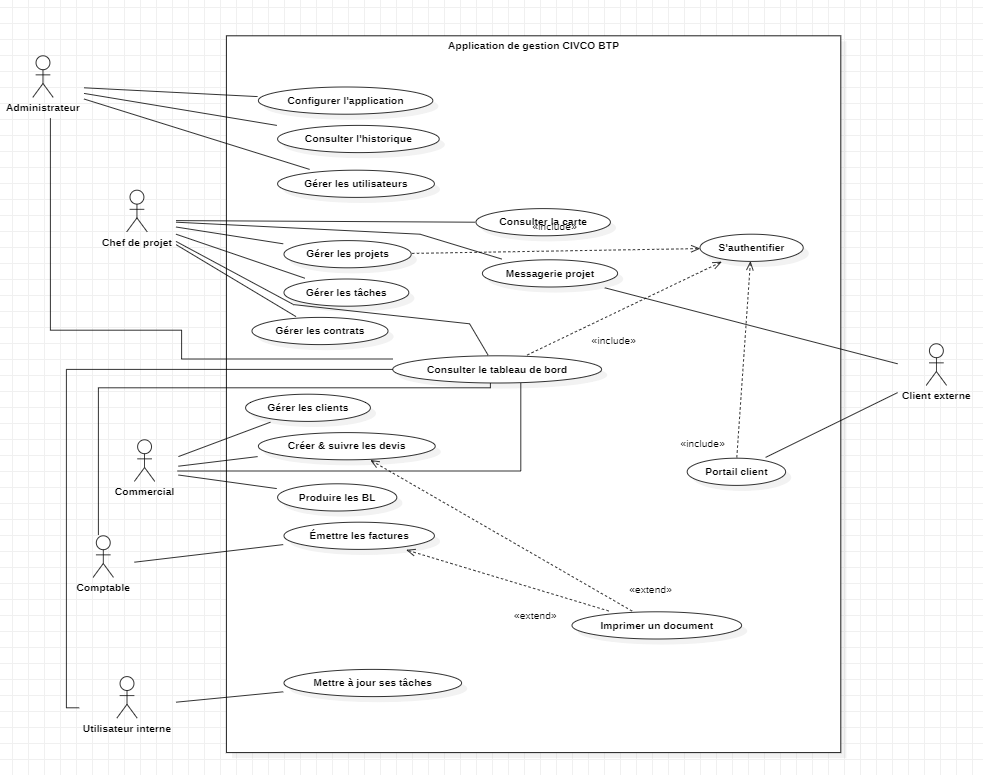
\includegraphics[width=\textwidth]{usecaseUML.png}
  \caption{Diagramme de cas d'utilisation de l'application CIVCO BTP}
  \label{fig:uc_diagram}
\end{figure}

\subsection{Diagramme de séquence}

Le diagramme de séquence (Figure~\ref{fig:seq_diagram}) illustre le scénario de création d'un devis par un
commercial. Les interactions mettent en évidence la séparation entre l'interface
React, l'API Laravel (validation, service métier) et la persistance en base de
données. Les étapes principales sont les suivantes :
\begin{enumerate}
  \item Le commercial s'authentifie via la SPA (cookie Sanctum + jeton CSRF).
  \item Il sélectionne un projet et saisit les lignes du devis.
  \item Le frontend envoie \texttt{POST /api/v1/quotes} avec les données JSON.
  \item Laravel valide la requête (Form Request), persiste le devis et ses lignes.
  \item L'API retourne une \texttt{QuoteResource} ; l'interface affiche la confirmation.
\end{enumerate}
Ce flux est représentatif du patron adopté sur l'ensemble des modules : le frontend
ne contient aucune logique métier critique ; la validation, les calculs et la
persistance sont toujours assurés côté serveur.

\medskip

D'autres scénarios de séquence ont été modélisés selon le même principe :
\textbf{conversion devis $\rightarrow$ facture} (contrôle du statut, transaction
base de données, copie des lignes), \textbf{signature de contrat} (génération
du PDF, capture de la signature canvas, mise à jour du statut) et
\textbf{assignation de tâche} (notification de l'utilisateur concerné).

\begin{figure}[H]
  \centering
  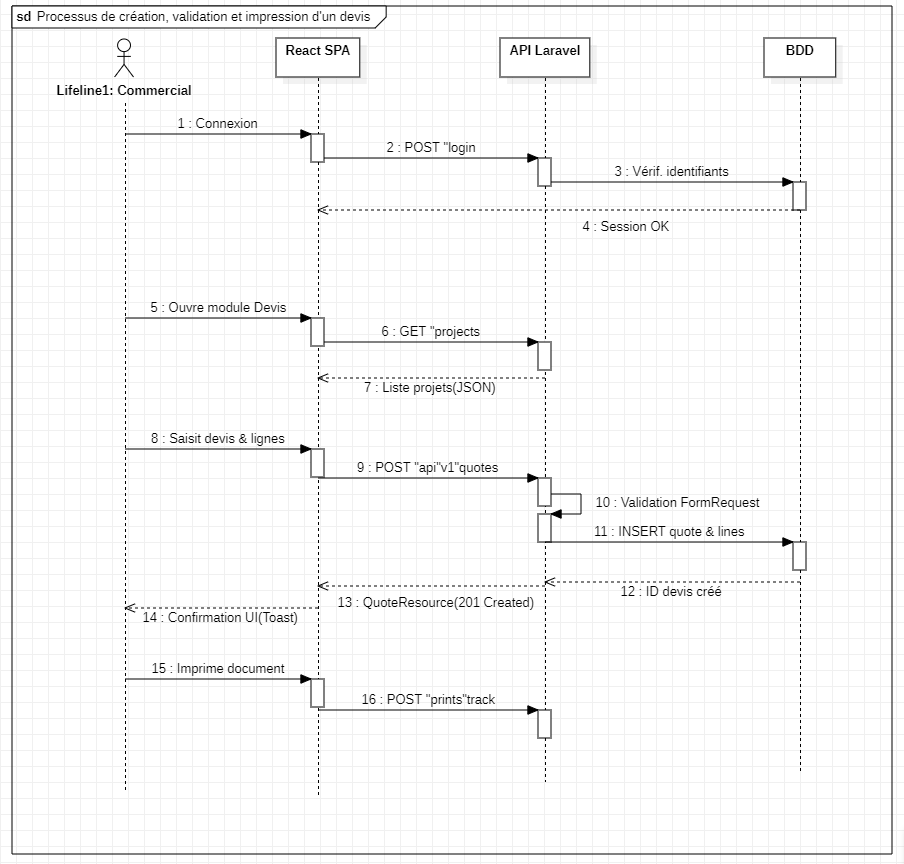
\includegraphics[width=\textwidth]{sequenceUML.png}
  \caption{Diagramme de séquence : création et enregistrement d'un devis}
  \label{fig:seq_diagram}
\end{figure}

\subsection{Diagramme de classes}

Le diagramme de classes (Figure~\ref{fig:class_diagram}) représente le modèle de données persistant simplifié.
Le Tableau~\ref{tab:classes} complète la description des entités principales et
de leurs relations.

\begin{figure}[H]
  \centering
  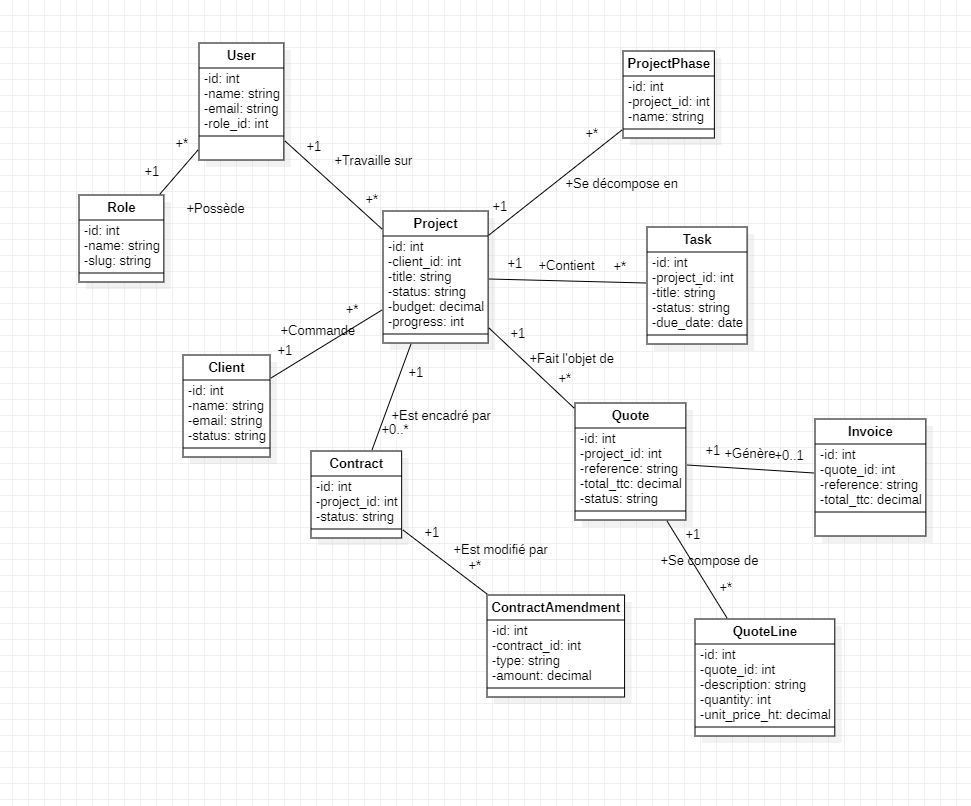
\includegraphics[width=\textwidth]{classeUML.png}
  \caption{Diagramme de classes simplifié du modèle de données métier}
  \label{fig:class_diagram}
\end{figure}

\begin{table}[H]
\caption{Description des classes et de leurs relations}
\label{tab:classes}
\centering
\small
\begin{tabular}{|l|p{4.8cm}|p{5.2cm}|}
\hline
\textbf{Classe} & \textbf{Attributs principaux} & \textbf{Relations} \\
\hline
\texttt{User} & id, name, email, role\_id & N User $\rightarrow$ 1 Role ;
N $\leftrightarrow$ N Project (équipe) \\
\hline
\texttt{Role} & id, name, slug & 1 Role $\rightarrow$ N Permission \\
\hline
\texttt{Client} & id, name, email, status & 1 Client $\rightarrow$ N Project ;
1 $\rightarrow$ N ClientContact \\
\hline
\texttt{Project} & id, client\_id, title, status, budget, progress & 1 $\rightarrow$ N Phase,
Task, Quote, Contract \\
\hline
\texttt{Quote} & id, project\_id, reference, total\_ttc, status & 1 $\rightarrow$ N QuoteLine ;
1 $\rightarrow$ 0..1 Invoice \\
\hline
\texttt{Invoice} & id, quote\_id, reference, total\_ttc & 1 $\rightarrow$ N InvoiceLine,
Payment \\
\hline
\texttt{Task} & id, project\_id, title, status, due\_date & N $\rightarrow$ 1 Project ;
N $\rightarrow$ 1 User (assigné) \\
\hline
\texttt{Contract} & id, project\_id, status & 1 $\rightarrow$ N ContractAmendment \\
\hline
\end{tabular}
\end{table}

\medskip

Le modèle met en évidence la \textbf{centralité du projet} : la plupart des entités
métier gravitent autour de \texttt{Project}, ce qui reflète l'organisation interne
de CIVCO BTP où le chantier constitue l'unité de travail de référence. Les
énumérations (\texttt{ProjectStatus}, \texttt{QuoteStatus}, \texttt{InvoiceStatus})
garantissent la cohérence des états dans l'application.

\subsection{Diagramme d'activité}

Le diagramme d'activité (Figure~\ref{fig:activity_diagram}) modélise le cycle de vie d'un projet de construction, depuis
sa création jusqu'à sa clôture. Le flux principal comprend : création du projet et
affectation du client, constitution de l'équipe et définition des phases, planification
des tâches, établissement du devis, signature du contrat, exécution des travaux avec
suivi d'avancement, facturation et clôture. Les points de décision portent sur
l'acceptation du devis et l'achèvement du projet ; en cas de refus, le devis peut
être révisé avant reprise du flux.

\vspace{0.4em}
\begin{center}
  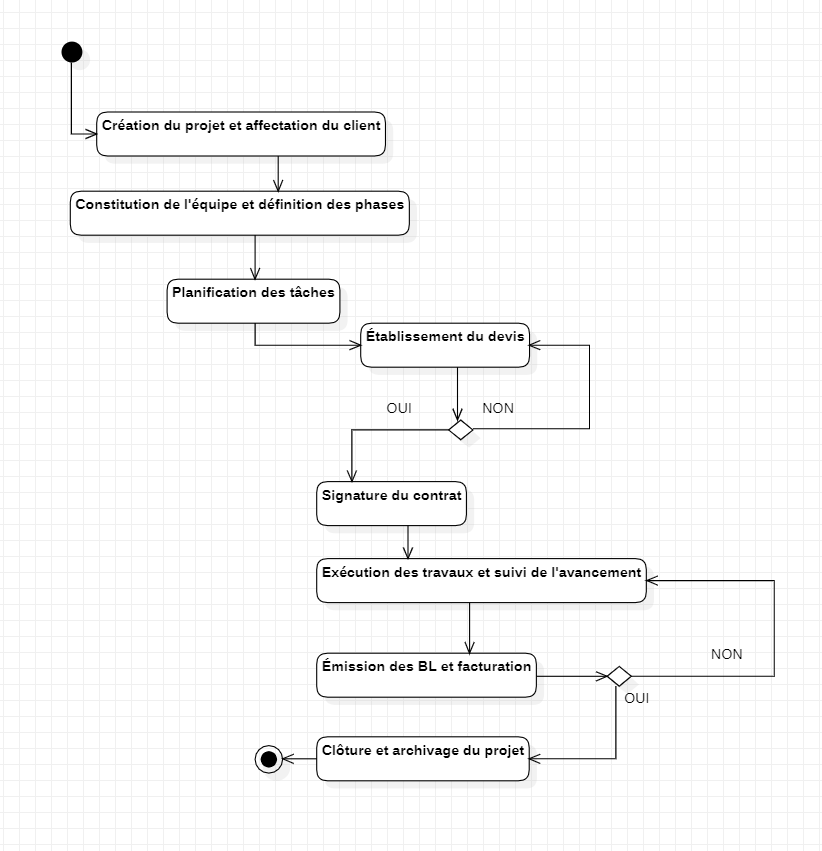
\includegraphics[height=0.50\textheight,keepaspectratio]{activiteUML.png}
  \captionof{figure}{Diagramme d'activité : cycle de vie d'un projet de construction}
  \label{fig:activity_diagram}
\end{center}

\newpage
\section*{Conclusion}

Ce chapitre a formalisé la conception de l'application de gestion de projets de
CIVCO BTP à travers trois niveaux d'abstraction complémentaires.

\medskip

Au niveau \textbf{fonctionnel}, l'analyse des besoins a identifié six acteurs métier,
vingt cas d'utilisation et treize exigences fonctionnelles couvrant l'ensemble du
cycle de vie d'un projet de construction : de la relation client à la facturation,
en passant par la planification des tâches et le suivi contractuel. Les neuf
exigences non-fonctionnelles fixent les contraintes de performance, de sécurité,
d'ergonomie et de maintenabilité auxquelles la solution doit répondre.

\medskip

Au niveau \textbf{architectural}, l'application repose sur une séparation nette en
trois couches : interface React en SPA, API Laravel exposant des services REST
sécurisés par Sanctum et RBAC, et persistance relationnelle via Eloquent. Le flux
d'authentification, la matrice des permissions et l'organisation modulaire du code
(backend par contrôleurs/services, frontend par features) garantissent une base
solide pour l'évolution future de l'outil.

\medskip

Au niveau \textbf{métier}, la conception détaillée des sept modules (projets, clients,
documents commerciaux, contrats, tâches, tableau de bord, portail client) traduit
les processus internes de CIVCO BTP en composants logiciels cohérents, avec des
règles de gestion explicites et des flux documentaires tracés.

\medskip

Enfin, la modélisation \textbf{UML} --- cas d'utilisation, séquence, classes et
activité --- formalise les interactions, le modèle de données et les flux métier,
et sert de référence pour la phase de réalisation décrite au chapitre suivant.

\medskip

Le chapitre suivant décrit l'implémentation concrète de cette conception : choix
d'environnement, structure du code, captures d'écran des modules principaux et
résultats de la campagne de tests.

\newpage

\chapter{Réalisation et Implémentation}
\label{chap:realisation}

\section{Introduction}

Ce chapitre décrit la réalisation concrète de l'application de gestion et de planification
des projets BTP développée pour CIVCO BTP, à partir de la conception présentée au
chapitre précédent. Nous présentons d'abord l'environnement technique et les outils
utilisés, puis détaillons l'implémentation du backend Laravel, du frontend React et
des principaux modules métier. Le chapitre se conclut par les tests réalisés et les
résultats de validation.

% ─────────────────────────────────────────────────────────────────────
\section{Environnement technique}

\subsection{Stack technologique}

\begin{description}
  \item[Serveur applicatif] PHP 8.3, Laravel 13.8, Laravel Sanctum 4
  (authentification SPA), Eloquent ORM, migrations et seeders.
  \item[Interface utilisateur] React 19.2, Vite 8, React Router 7, Tailwind CSS 4, Axios,
  Recharts (graphiques), Leaflet (cartographie).
  \item[Base de données] MySQL / PostgreSQL (modèle relationnel,
  schéma versionné par migrations Laravel).
  \item[Outils complémentaires] Git / GitHub (versionnement), Visual Studio Code (IDE),
  PHPUnit 12 (tests backend), ESLint (qualité frontend).
\end{description}

Le Tableau~\ref{tab:stack_versions} récapitule les versions principales des composants
utilisés en développement.

\begin{table}[H]
\caption{Versions des composants de la stack technique}
\label{tab:stack_versions}
\centering
\small
\begin{tabular}{|l|l|p{6.5cm}|}
\hline
\textbf{Composant} & \textbf{Version} & \textbf{Rôle} \\
\hline
PHP & 8.3+ & Langage backend, exécution Laravel \\
\hline
Laravel & 13.8 & Framework API, ORM, authentification \\
\hline
Laravel Sanctum & 4.x & Sessions SPA sécurisées \\
\hline
React & 19.2 & Interface utilisateur composants \\
\hline
Vite & 8.0 & Build tool et serveur de développement \\
\hline
Tailwind CSS & 4.3 & Styles utilitaires \\
\hline
MySQL / PostgreSQL & 8.x / 16 & Persistance relationnelle \\
\hline
PHPUnit & 12.5 & Tests automatisés backend \\
\hline
\end{tabular}
\end{table}

\subsection{Outils de développement}

\begin{description}
  \item[Gestion de projet] Trello (tableau Kanban) pour planifier les modules,
  suivre l'avancement des tâches et préparer les démonstrations de suivi.
  \item[Contrôle de version] Git et GitHub pour le suivi des évolutions, branches de
  fonctionnalités et revues de code.
  \item[IDE] Visual Studio Code avec extensions PHP Intelephense, ESLint et Prettier.
  \item[Tests] PHPUnit pour les tests d'intégration API ; tests manuels sur navigateur
  (Chrome, Edge) pour les parcours utilisateurs.
  \item[Qualité de code] Laravel Pint (formatage PHP), ESLint (linting JavaScript/React).
  \item[Documentation API] Routes Laravel exposées sous \texttt{/api/v1/}, testables via
  outils HTTP (Postman, curl) ou le navigateur pour les endpoints GET.
\end{description}

\subsection{Architecture de déploiement}

\subsubsection{Environnement de développement}

En développement, l'application repose sur deux processus parallèles, orchestrés depuis
deux terminaux :

\begin{enumerate}
  \item \textbf{Backend Laravel} : \texttt{php artisan serve --host=127.0.0.1 --port=8000}
  expose l'API sur le port 8000.
  \item \textbf{Frontend Vite} : \texttt{npm run dev} lance le serveur de développement
  React sur le port 5173, avec rechargement à chaud (\textit{hot-reload}).
\end{enumerate}

Le fichier \texttt{vite.config.js} configure un proxy : les requêtes vers \texttt{/api},
\texttt{/sanctum} et \texttt{/storage} sont redirigées vers Laravel (port 8000), ce qui
évite les problèmes de CORS en développement et simule un déploiement unifié.

\subsubsection{Schéma de communication}

\begin{itemize}
  \item Le navigateur charge l'application React depuis \texttt{http://127.0.0.1:5173}.
  \item Les appels API transitent par le proxy Vite vers \texttt{http://127.0.0.1:8000/api/v1/}.
  \item Sanctum émet un cookie de session après authentification ; Axios est configuré
  avec \texttt{withCredentials: true}.
  \item Les fichiers uploadés (logos, documents, signatures) sont stockés dans
  \texttt{storage/app/public} et servis via le lien symbolique \texttt{public/storage}.
\end{itemize}

\subsubsection{Étude d'hébergement : OVHcloud vs o2switch}

En vue d'une mise en production chez CIVCO BTP, une \textbf{étude comparative
d'hébergement} a été menée entre deux prestataires français largement utilisés pour
les applications web PHP : \textbf{OVHcloud} et \textbf{o2switch}. L'objectif était
d'identifier la solution la mieux adaptée au profil de l'entreprise : application
métier interne, équipe réduite, budget maîtrisé et besoin de simplicité
d'administration.

\medskip

Les critères d'évaluation retenus sont les suivants :

\begin{itemize}
  \item \textbf{Compatibilité Laravel / PHP 8.3} : exécution de l'API backend et des
  commandes \texttt{artisan} (migrations, files d'attente, planificateur).
  \item \textbf{Base de données} : support MySQL ou PostgreSQL, sauvegardes et quotas.
  \item \textbf{Déploiement du frontend React} : hébergement des fichiers statiques
  produits par \texttt{npm run build}.
  \item \textbf{Sécurité} : certificat SSL, pare-feu, mises à jour système.
  \item \textbf{Coût et prévisibilité} : tarification mensuelle, absence de surprises
  sur la facturation.
  \item \textbf{Support et localisation} : assistance en français, datacenters en
  France, conformité pour des données clients BTP.
  \item \textbf{Facilité d'exploitation} : courbe d'apprentissage pour une PME sans
  équipe DevOps dédiée.
\end{itemize}

\begin{table}[H]
\caption{Comparatif d'hébergement : OVHcloud vs o2switch}
\label{tab:hebergement}
\centering
\small
\begin{tabular}{|p{3.2cm}|p{5.2cm}|p{5.2cm}|}
\hline
\textbf{Critère} & \textbf{OVHcloud} & \textbf{o2switch} \\
\hline
Type d'offre & VPS, cloud public, serveurs dédiés (IaaS) & Hébergement mutualisé
tout-en-un \\
\hline
Laravel / PHP & Compatible (configuration manuelle : Nginx, PHP-FPM, Composer) &
Compatible nativement (PHP 8.x, SSH, Composer) \\
\hline
Base de données & MySQL/PostgreSQL à installer et administrer & MySQL inclus,
bases multiples \\
\hline
Frontend React (build) & Fichiers statiques sur VPS ou Object Storage & Hébergement
direct des assets \texttt{dist/} \\
\hline
SSL (HTTPS) & Let's Encrypt ou certificat payant (selon offre) & Let's Encrypt
inclus et automatisé \\
\hline
Sauvegardes & À configurer (snapshots, scripts) & Sauvegardes journalières incluses \\
\hline
Tarification & Variable (facturation à l'usage, snapshots, trafic) & Forfait fixe
illimité (offre unique) \\
\hline
Support & Tickets, documentation technique & Support français réactif, panel cPanel \\
\hline
Scalabilité & Élevée (montée en charge horizontale) & Modérée (mutualisé, adapté PME) \\
\hline
Complexité admin & Élevée (sysadmin requis) & Faible (panel graphique) \\
\hline
\end{tabular}
\end{table}

\medskip

\textbf{Analyse.} OVHcloud~\cite{ovhcloud} offre une grande flexibilité et une
scalabilité adaptée aux applications à fort trafic ou aux architectures distribuées
(conteneurs Docker, load balancing, bases managées). En revanche, le déploiement d'une
application Laravel + React sur un VPS OVHcloud suppose une configuration manuelle
du serveur web, de PHP-FPM, des certificats, des sauvegardes et de la supervision.
Cette approche est pertinente pour des équipes disposant de compétences
d'administration système, mais elle représente un surcoût en temps pour une PME comme
CIVCO BTP.

\medskip

o2switch~\cite{o2switch}, hébergeur français basé à Grabels, propose une offre
mutualisée orientée simplicité : PHP récent, bases MySQL, certificats SSL gratuits,
sauvegardes automatiques et support technique francophone. Pour une application métier
interne au volume d'utilisateurs modéré (équipes CIVCO BTP et clients portail), cette
formule couvre les besoins sans nécessiter la gestion d'un serveur virtuel. Le frontend
React est déployé sous forme de fichiers statiques (\texttt{npm run build}), tandis que
Laravel gère l'API et les sessions Sanctum sur le même domaine, simplifiant la
configuration des cookies et du CSRF.

\medskip

\textbf{Choix retenu.} Au terme de cette étude, \textbf{o2switch} a été retenu comme
plateforme d'hébergement cible pour CIVCO BTP. Ce choix se justifie par :

\begin{itemize}
  \item un \textbf{rapport qualité/prix} favorable pour une application interne ;
  \item une \textbf{mise en production plus rapide}, sans administration système
  avancée ;
  \item une \textbf{compatibilité native} avec la stack Laravel / MySQL ;
  \item un \textbf{support en français} et des datacenters localisés en France ;
  \item des \textbf{sauvegardes et SSL inclus}, répondant aux exigences de sécurité
  identifiées au Chapitre~3.
\end{itemize}

OVHcloud reste une alternative crédible si l'application devait évoluer vers une
architecture plus complexe (montée en charge importante, microservices, conteneurisation
Docker). Pour la première version de l'outil, la simplicité opérationnelle d'o2switch
a été privilégiée.

\subsubsection{Configuration : variables d'environnement}

La configuration sensible est centralisée dans le fichier \texttt{.env} du backend.
Le Tableau~\ref{tab:env_vars} liste les variables principales :

\begin{table}[H]
\caption{Variables d'environnement principales du fichier \texttt{.env}}
\label{tab:env_vars}
\centering
\small
\begin{tabular}{|l|p{7.5cm}|}
\hline
\textbf{Variable} & \textbf{Rôle} \\
\hline
\texttt{APP\_URL} & URL publique de l'application (ex. \texttt{http://127.0.0.1:8000}) \\
\hline
\texttt{DB\_CONNECTION / DB\_DATABASE} & Connexion SGBD (MySQL ou PostgreSQL) \\
\hline
\texttt{SESSION\_DRIVER} & Pilote de session (fichier ou base de données) \\
\hline
\texttt{SANCTUM\_STATEFUL\_DOMAINS} & Domaines autorisés pour les cookies Sanctum \\
\hline
\texttt{FRONTEND\_URL} & URL du frontend (pour les redirections et CORS) \\
\hline
\texttt{MAIL\_*} & Configuration SMTP (notifications, invitations portail) \\
\hline
\end{tabular}
\end{table}

\subsubsection{Initialisation de la base de données}

Le démarrage d'un environnement neuf suit la séquence standard Laravel :

\begin{enumerate}
  \item \texttt{composer install} : installation des dépendances PHP.
  \item \texttt{cp .env.example .env} puis configuration de la base de données.
  \item \texttt{php artisan key:generate} : génération de la clé d'application.
  \item \texttt{php artisan migrate --seed} : création du schéma et données de démonstration.
  \item \texttt{php artisan storage:link} : lien symbolique pour les fichiers publics.
\end{enumerate}

Les seeders (\texttt{DatabaseSeeder}, \texttt{DemoSeeder}, \texttt{RoleSeeder}) peuplent
la base avec des utilisateurs de test, des rôles, des permissions, des clients et des
projets représentatifs du secteur BTP au Maroc.

% ─────────────────────────────────────────────────────────────────────
\section{Implémentation du backend}

\subsection{Structure du projet}

Le backend suit l'architecture modulaire Laravel, organisée par responsabilité :

\begin{verbatim}
backend/
+-- app/
|   +-- Enums/              # Statuts (Project, Quote, Invoice, Client...)
|   +-- Http/
|   |   +-- Controllers/Api/V1/   # ~45 controleurs REST
|   |   +-- Middleware/           # Auth, permissions, contexte
|   |   +-- Requests/             # Validation par domaine
|   |   +-- Resources/            # Serialisation JSON
|   +-- Models/             # Entites Eloquent (~35 modeles)
|   +-- Services/           # Logique metier (QuoteService, etc.)
+-- database/
|   +-- migrations/         # ~70 migrations versionnees
|   +-- seeders/            # Donnees de demo et referentiels
+-- routes/api.php          # Definition des routes /api/v1/
\-- tests/Feature/          # Tests PHPUnit d'integration
\end{verbatim}

Cette organisation sépare clairement le transport HTTP (contrôleurs), la validation
(Requests), la transformation des réponses (Resources) et la logique métier (Services),
conformément au patron décrit au Chapitre~3.

\subsection{API REST : endpoints principaux}

L'API est regroupée sous le préfixe \texttt{/api/v1/}. Les endpoints principaux sont
organisés par domaine fonctionnel :

\begin{description}
  \item[Authentification] \texttt{POST /login}, \texttt{GET /me}, \texttt{POST /logout},
  \texttt{PATCH /me} (profil utilisateur). Gestion de session via Sanctum.
  \item[Projets] \texttt{GET/POST /projects}, \texttt{GET/PATCH/DELETE /projects/\{id\}},
  gestion des phases, équipe, dépenses, médias et commentaires.
  \item[Clients] \texttt{GET/POST /clients}, archivage, contacts, provisionnement
  portail (\texttt{POST /clients/\{id\}/portal-account}).
  \item[Devis] \texttt{GET/POST /quotes}, lignes de détail, conversion en facture,
  suivi des statuts et impressions.
  \item[Factures] \texttt{GET/POST /invoices}, paiements, état de facturation.
  \item[Bons de livraison] \texttt{GET/POST /delivery-forms}, lignes et statuts.
  \item[Contrats] \texttt{GET/POST /contracts}, compilation, signature, avenants
  (\texttt{/contract-amendments}).
  \item[Tâches] \texttt{GET/POST /tasks}, assignation, filtrage par projet et utilisateur.
  \item[Équipe] \texttt{GET /team/members}, gestion des membres et rôles.
  \item[Configuration] \texttt{/roles}, \texttt{/document-templates},
  \texttt{/tenant/document-controls}, thème et badges.
  \item[Tableau de bord] \texttt{GET /dashboard/summary}, indicateurs agrégés.
  \item[Recherche] \texttt{GET /search}, recherche globale multi-entités.
  \item[Portail client] \texttt{/client-portal/*} : projets, devis, contrats,
  messagerie, acceptation et signature.
  \item[Historique] \texttt{GET /activity-logs}, journal des actions.
\end{description}

Chaque route métier sensible est protégée par le middleware \texttt{permission:*},
qui vérifie que l'utilisateur authentifié dispose du droit requis avant d'exécuter
l'action.

\subsection{Services métier}

La logique complexe est extraite des contrôleurs vers des classes Service :

\begin{itemize}
  \item \textbf{QuoteService / InvoiceService} : calcul des totaux, numérotation,
  conversion devis $\rightarrow$ facture, gestion des statuts.
  \item \textbf{DeliveryFormService} : production des bons de livraison et liaison
  aux projets.
  \item \textbf{DocumentService / DocumentTemplateCompilationService} : génération
  et compilation des documents à partir de modèles.
  \item \textbf{DashboardService} : agrégation des indicateurs (projets actifs,
  tâches en retard, chiffre d'affaires).
  \item \textbf{AuthContextService} : résolution du contexte utilisateur (rôles,
  permissions, société courante).
  \item \textbf{ActivityLogService} : journalisation des actions sensibles.
  \item \textbf{PrintTrackingService} : suivi des impressions officielles et quotas.
  \item \textbf{SiteGeocodingService} : géolocalisation des chantiers (Nominatim +
  coordonnées de repli pour les villes marocaines).
\end{itemize}

\subsection{Authentification et contrôle d'accès}

L'authentification repose sur \textbf{Laravel Sanctum} en mode SPA :

\begin{enumerate}
  \item Le frontend obtient un cookie CSRF via \texttt{GET /sanctum/csrf-cookie}.
  \item L'utilisateur envoie ses identifiants à \texttt{POST /api/v1/login}.
  \item Laravel valide, crée une session et retourne le profil (\texttt{UserResource})
  avec rôles et permissions.
  \item Chaque requête ultérieure inclut le cookie de session ; le middleware
  \texttt{auth:sanctum} protège les routes.
  \item Le middleware \texttt{permission:slug} vérifie les droits granulaires
  (\texttt{project.view}, \texttt{quote.manage}, etc.).
\end{enumerate}

Le service \texttt{PostLoginRedirectService} oriente l'utilisateur vers la page
d'accueil adaptée à son profil (tableau de bord admin, liste des projets pour un
chef de projet, factures pour un comptable).

\subsection{Migrations et modèle de données}

Le schéma de base compte environ 70 migrations, couvrant l'ensemble des entités métier.
Les migrations sont idempotentes et versionnées : chaque modification de schéma
produit un nouveau fichier daté, exécutable de façon reproductible sur tout
environnement.

\medskip

Les relations Eloquent principales ont été implémentées comme suit :
\begin{itemize}
  \item \texttt{Client} \texttt{hasMany} \texttt{Project}
  \item \texttt{Project} \texttt{belongsTo} \texttt{Client}, \texttt{hasMany} \texttt{ProjectPhase},
  \texttt{Task}, \texttt{Quote}, \texttt{Contract}
  \item \texttt{Quote} \texttt{hasMany} \texttt{QuoteLine}, \texttt{hasOne} \texttt{Invoice}
  \item \texttt{User} \texttt{belongsToMany} \texttt{Project} (équipe), \texttt{belongsTo} \texttt{Role}
\end{itemize}

Les \textbf{API Resources} (\texttt{ProjectResource}, \texttt{QuoteResource}, etc.)
contrôlent les champs exposés au frontend et permettent d'inclure conditionnellement
les relations (\texttt{client}, \texttt{lines}, \texttt{teamMembers}).

\subsection{Middleware et sécurité des routes}

Le pipeline de middleware Laravel applique une chaîne de vérifications sur chaque
requête API protégée :

\begin{enumerate}
  \item \textbf{auth:sanctum} : vérifie que l'utilisateur est authentifié via session.
  \item \textbf{EnsureCompanyContext} : résout la société courante à partir de
  l'en-tête \texttt{X-Company-Id} ou du contexte utilisateur.
  \item \textbf{permission:slug} : contrôle granulaire par action métier
  (\texttt{client.view}, \texttt{invoice.manage}, etc.).
  \item \textbf{ValidateCsrfToken} : protection contre les requêtes forgées sur
  les verbes mutants (\texttt{POST}, \texttt{PUT}, \texttt{PATCH}, \texttt{DELETE}).
\end{enumerate}

Cette approche en profondeur (\textit{defense in depth}) garantit qu'aucune action
métier ne peut être exécutée sans authentification et sans autorisation explicite,
conformément aux bonnes pratiques de sécurité web~\cite{owasp}.

\subsection{Exemple : création d'un devis}

Le flux de création d'un devis illustre l'interaction entre les couches :

\begin{enumerate}
  \item Le frontend envoie \texttt{POST /api/v1/quotes} avec le corps JSON
  (client, projet, lignes, montants).
  \item \texttt{StoreQuoteRequest} valide les champs (références obligatoires,
  montants positifs, dates cohérentes).
  \item \texttt{QuoteController@store} délègue à \texttt{QuoteService::create()}.
  \item Le service crée l'enregistrement \texttt{Quote} et ses \texttt{QuoteLine}
  associées dans une transaction base de données.
  \item Les totaux HT, TVA et TTC sont calculés automatiquement.
  \item \texttt{QuoteResource} sérialise la réponse JSON pour le frontend.
  \item \texttt{ActivityLogService} journalise l'action si configuré.
\end{enumerate}

Ce patron (Request $\rightarrow$ Controller $\rightarrow$ Service $\rightarrow$
Resource) est reproduit sur l'ensemble des modules métier.

\subsection{Modules complémentaires}

En complément des modules principaux, plusieurs fonctionnalités transverses ont été
implémentées :

\medskip

\textbf{Notifications :} le modèle \texttt{Notification} et le contrôleur associé
permettent d'informer les utilisateurs des événements importants (nouvelle tâche
assignée, devis accepté, message reçu). L'interface affiche un badge de notification
non lue dans l'en-tête.

\medskip

\textbf{Messagerie :} le module \texttt{PortalMessage} gère les échanges entre
l'équipe interne et les clients externes, scopés par projet. Le service
\texttt{PortalMessageService} filtre les conversations selon les droits de
l'utilisateur (\texttt{can\_chat\_with\_client} sur les membres d'équipe).

\medskip

\textbf{Recherche globale :} le composant \texttt{GlobalSearch} et l'endpoint
\texttt{GET /search} permettent de retrouver rapidement un client, un projet, un
devis ou une facture par mot-clé, améliorant la productivité au quotidien.

\medskip

\textbf{Contrôle d'impression :} \texttt{PrintTrackingService} gère les quotas
d'impressions officielles par type de document et par en-tête (avec ou sans papier
à en-tête). Au-delà du quota, les impressions sont marquées « COPIE - NON OFFICIEL ».

\medskip

\textbf{Journal d'activité :} chaque action sensible (création de projet, validation
de devis, archivage client) est enregistrée par \texttt{ActivityLogService} avec
l'identité de l'utilisateur, le type d'action et l'horodatage. Le module
\texttt{features/history/} expose ces entrées sous forme de fil d'audit consultable
par l'administrateur.

\medskip

\textbf{Géocodage des chantiers :} lors de la saisie d'une adresse de chantier,
\texttt{SiteGeocodingService} tente de résoudre automatiquement les coordonnées
GPS via l'API Nominatim (OpenStreetMap). En cas d'échec, un référentiel de
coordonnées des principales villes marocaines (\texttt{MoroccoCityCoordinates})
assure un positionnement approximatif sur la carte Leaflet.

\medskip

\textbf{Modèles de documents :} le module \texttt{DocumentTemplate} permet de
définir des gabarits de contrats et de documents commerciaux avec des champs
dynamiques (placeholders). Le service \texttt{DocumentTemplateCompilationService}
injecte les données du projet et du client lors de la génération du document final.

\medskip

\textbf{Gestion d'équipe :} \texttt{TeamMemberService} et \texttt{TeamQueryService}
centralisent l'affectation des collaborateurs aux projets, la gestion des rôles
sur chantier et le contrôle de l'autorisation de messagerie client
(\texttt{can\_chat\_with\_client}).

% ─────────────────────────────────────────────────────────────────────
\section{Implémentation du frontend}

\subsection{Architecture React}

Le frontend est une SPA React 19 organisée par domaines métier (\textit{features}) :

\begin{verbatim}
frontend/src/
+-- api/                    # Modules Axios par ressource
|   +-- client.js           # Instance Axios + intercepteurs
|   +-- projects.js, clients.js, quotes.js, invoices.js...
+-- components/             # Composants transverses (Sidebar, Modal...)
+-- context/
|   +-- AuthContext.jsx     # Session, roles, permissions
|   +-- ThemeContext.jsx    # Theme sombre, couleurs societe
|   +-- LanguageContext.jsx # i18n FR / EN
+-- features/
|   +-- dashboard/          # Tableau de bord et widgets
|   +-- projects/           # Liste, detail, phases, equipe
|   +-- clients/            # Gestion clients et portail
|   +-- quotes/             # Devis
|   +-- invoices/           # Factures
|   +-- delivery-forms/     # Bons de livraison
|   +-- tasks/              # Taches
|   +-- configuration/      # Parametres, roles, modeles
|   +-- profile/            # Profil utilisateur
+-- routes/
|   +-- AppRoutes.jsx       # Definition des routes
|   +-- routePermissions.js # Controle d'acces par route
\-- i18n/locales/           # Traductions fr.js, en.js
\end{verbatim}

\subsection{Client HTTP et authentification}

Le module \texttt{api/client.js} centralise la configuration Axios :

\begin{itemize}
  \item \texttt{baseURL} pointant vers \texttt{/api/v1} (proxifié par Vite).
  \item \texttt{withCredentials: true} pour transmettre les cookies Sanctum.
  \item Intercepteur de requête : récupération du jeton CSRF depuis le cookie
  \texttt{XSRF-TOKEN} et injection dans l'en-tête \texttt{X-XSRF-TOKEN}.
  \item Intercepteur de réponse : redirection vers \texttt{/login} en cas de
  \texttt{401 Unauthorized}.
  \item En-tête \texttt{X-Company-Id} pour le contexte société lorsque requis.
\end{itemize}

Le \texttt{AuthContext} expose l'état global d'authentification : utilisateur courant,
rôles, permissions, fonctions \texttt{login} / \texttt{logout}, et helpers de
vérification des droits consommés par les composants \texttt{PermissionGate} et
\texttt{AdminRoute}.

\subsection{Routage et contrôle d'accès}

\texttt{AppRoutes.jsx} définit l'arborescence de navigation :

\begin{itemize}
  \item Routes publiques : \texttt{/login}.
  \item Routes authentifiées : \texttt{/} (dashboard), \texttt{/projects},
  \texttt{/clients}, \texttt{/quotes}, \texttt{/invoices}, \texttt{/tasks},
  \texttt{/map}, \texttt{/configuration}, \texttt{/history}.
  \item Portail client : \texttt{/portal/*} (interface dédiée aux clients externes).
  \item Protection : composants \texttt{ProtectedRoute}, \texttt{AdminRoute} et
  fonction \texttt{canAccessRoute()} qui croise le chemin demandé avec les
  permissions de l'utilisateur.
\end{itemize}

\subsection{Composants transverses}

Plusieurs composants partagés structurent l'expérience utilisateur :

\begin{itemize}
  \item \textbf{Sidebar} : navigation principale, filtrée selon les permissions.
  \item \textbf{AppLayout} : enveloppe commune (sidebar + en-tête + contenu).
  \item \textbf{GlobalSearch} : recherche unifiée clients, projets, documents.
  \item \textbf{CommercialPrintSheet} : génération et impression des documents
  commerciaux (devis, factures, BL) avec suivi des impressions.
  \item \textbf{PrintOptionsModal} : choix d'impression (avec/sans en-tête,
  copie officielle).
\end{itemize}

\subsection{Internationalisation}

L'application supporte le français (par défaut) et l'anglais via \texttt{LanguageContext}
et les fichiers \texttt{i18n/locales/fr.js} et \texttt{en.js}. Les libellés de
l'interface, les messages d'erreur et les intitulés de menus sont externalisés,
facilitant l'ajout de nouvelles langues.

\subsection{Détail des modules frontend}

Chaque module \textit{feature} suit une structure cohérente : une page liste
(\texttt{*Page.jsx}), une ou plusieurs pages détail (\texttt{*DetailPage.jsx}),
des composants locaux (\texttt{components/}) et un module API dédié
(\texttt{api/*.js}).

\medskip

\textbf{Module Projets} (\texttt{features/projects/}) : \texttt{ProjectsPage} affiche
la liste filtrable des chantiers ; \texttt{ProjectDetailPage} regroupe les onglets
phases, tâches, équipe, documents et contrats. Le composant \texttt{ProjectAmendmentsTab}
gère les avenants contractuels.

\medskip

\textbf{Module Clients} (\texttt{features/clients/}) : \texttt{ClientsPage} avec
recherche et filtres ; \texttt{NewClientModal} pour la création ; \texttt{ClientPortalPanel}
pour la gestion de l'accès portail. Le composant \texttt{ConfirmArchiveModal} sécurise
l'archivage.

\medskip

\textbf{Module Documents commerciaux} : \texttt{QuotesPage}, \texttt{QuoteDetailPage},
\texttt{InvoicesPage}, \texttt{DeliveryFormDetailPage}. Les composants d'impression
(\texttt{CommercialPrintSheet}, \texttt{DeliveryFormPrintSheet}) génèrent les
versions PDF imprimables.

\medskip

\textbf{Module Configuration} (\texttt{features/configuration/}) : panneaux dédiés
pour les rôles (\texttt{RolesSettingsPanel}), les modèles de contrats
(\texttt{ContractTemplateSettingsPanel}), les contrôles d'impression
(\texttt{DocumentControlsSettingsPanel}) et les modèles de documents
(\texttt{DocumentTemplatesSettingsPanel}).

\subsection{Gestion d'état et hooks}

L'état applicatif repose principalement sur React Context :

\begin{itemize}
  \item \textbf{AuthContext} : session utilisateur, permissions, fonctions login/logout.
  \item \textbf{ThemeContext} : couleurs de la société injectées en variables CSS.
  \item \textbf{LanguageContext} : bascule FR / EN de l'interface.
  \item \textbf{usePolicyPrint / useProjectTasks} : hooks métier encapsulant la
  logique d'impression et de chargement des tâches projet.
\end{itemize}

React Query (\texttt{@tanstack/react-query}) est installé et prêt pour le cache
des requêtes API ; son adoption progressive permettra d'optimiser les rechargements
de listes et fiches détail.

% ─────────────────────────────────────────────────────────────────────
\section{Déroulement du développement et livrables}

\subsection{Phases de réalisation}

Le développement a suivi la planification définie au Chapitre~1, avec une
progression par modules fonctionnels. Chaque phase a produit un incrément
démontrable lors des réunions de suivi hebdomadaires avec l'encadrant professionnel.

\begin{table}[H]
\caption{Phases de développement et modules livrés}
\label{tab:livrables}
\centering
\small
\begin{tabular}{|l|p{5.5cm}|p{5.5cm}|}
\hline
\textbf{Phase} & \textbf{Modules livrés} & \textbf{Validation} \\
\hline
Fondations & Auth Sanctum, RBAC, navigation React, layout & Connexion multi-profils \\
\hline
Cœur métier & Projets, clients, phases, équipe & CRUD complet, carte \\
\hline
Documents & Devis, factures, BL, impression & Cycle commercial bout en bout \\
\hline
Opérations & Tâches, contrats, avenants, dépenses & Suivi opérationnel \\
\hline
Collaboration & Portail client, messagerie, notifications & Parcours client externe \\
\hline
Gouvernance & Configuration, historique, recherche globale & Administration complète \\
\hline
\end{tabular}
\end{table}

\subsection{Synthèse quantitative des livrables}

Au terme du stage, l'application comprend les éléments quantitatifs suivants,
illustrant l'ampleur de la réalisation :

\begin{itemize}
  \item Plus de \textbf{70 migrations} de base de données versionnées.
  \item Environ \textbf{40 contrôleurs API} et \textbf{25 services métier}.
  \item Plus de \textbf{30 modules frontend} (\textit{features} et composants).
  \item Une suite de \textbf{7 classes de tests} PHPUnit couvrant les flux critiques.
  \item Plus de \textbf{200 routes API} protégées par middleware d'authentification
  et de permissions.
  \item Support \textbf{bilingue} (français / anglais) sur l'ensemble de l'interface.
\end{itemize}

\subsection{Bonnes pratiques adoptées}

Plusieurs bonnes pratiques de génie logiciel ont été appliquées tout au long du
développement :

\begin{itemize}
  \item \textbf{Séparation des responsabilités} : contrôleurs fins, logique métier
  dans les services, validation dans les Form Requests.
  \item \textbf{Conventions de nommage} : respect des standards Laravel (PascalCase
  pour les classes, snake\_case pour les colonnes) et React (PascalCase pour les
  composants).
  \item \textbf{Versionnement Git} : branches par fonctionnalité, commits atomiques,
  messages descriptifs.
  \item \textbf{Suivi Kanban (Trello)} : chaque module ou correction était modélisé
  sous forme de carte, déplacée au fil de l'avancement entre les colonnes du tableau.
  \item \textbf{Revue de code} : validation des choix techniques avec l'encadrant
  professionnel avant intégration des modules sensibles (facturation, permissions).
  \item \textbf{Documentation inline} : commentaires sur les règles métier non
  évidentes, docblocks sur les méthodes de service exposées à l'API.
\end{itemize}

% ─────────────────────────────────────────────────────────────────────
\section{Interfaces principales}

Cette section présente les écrans clés de l'application. Les captures d'écran seront
insérées ultérieurement ; les descriptions ci-dessous reflètent l'implémentation
actuelle.

\subsection{Page de connexion}

\begin{figure}[H]
  \centering
  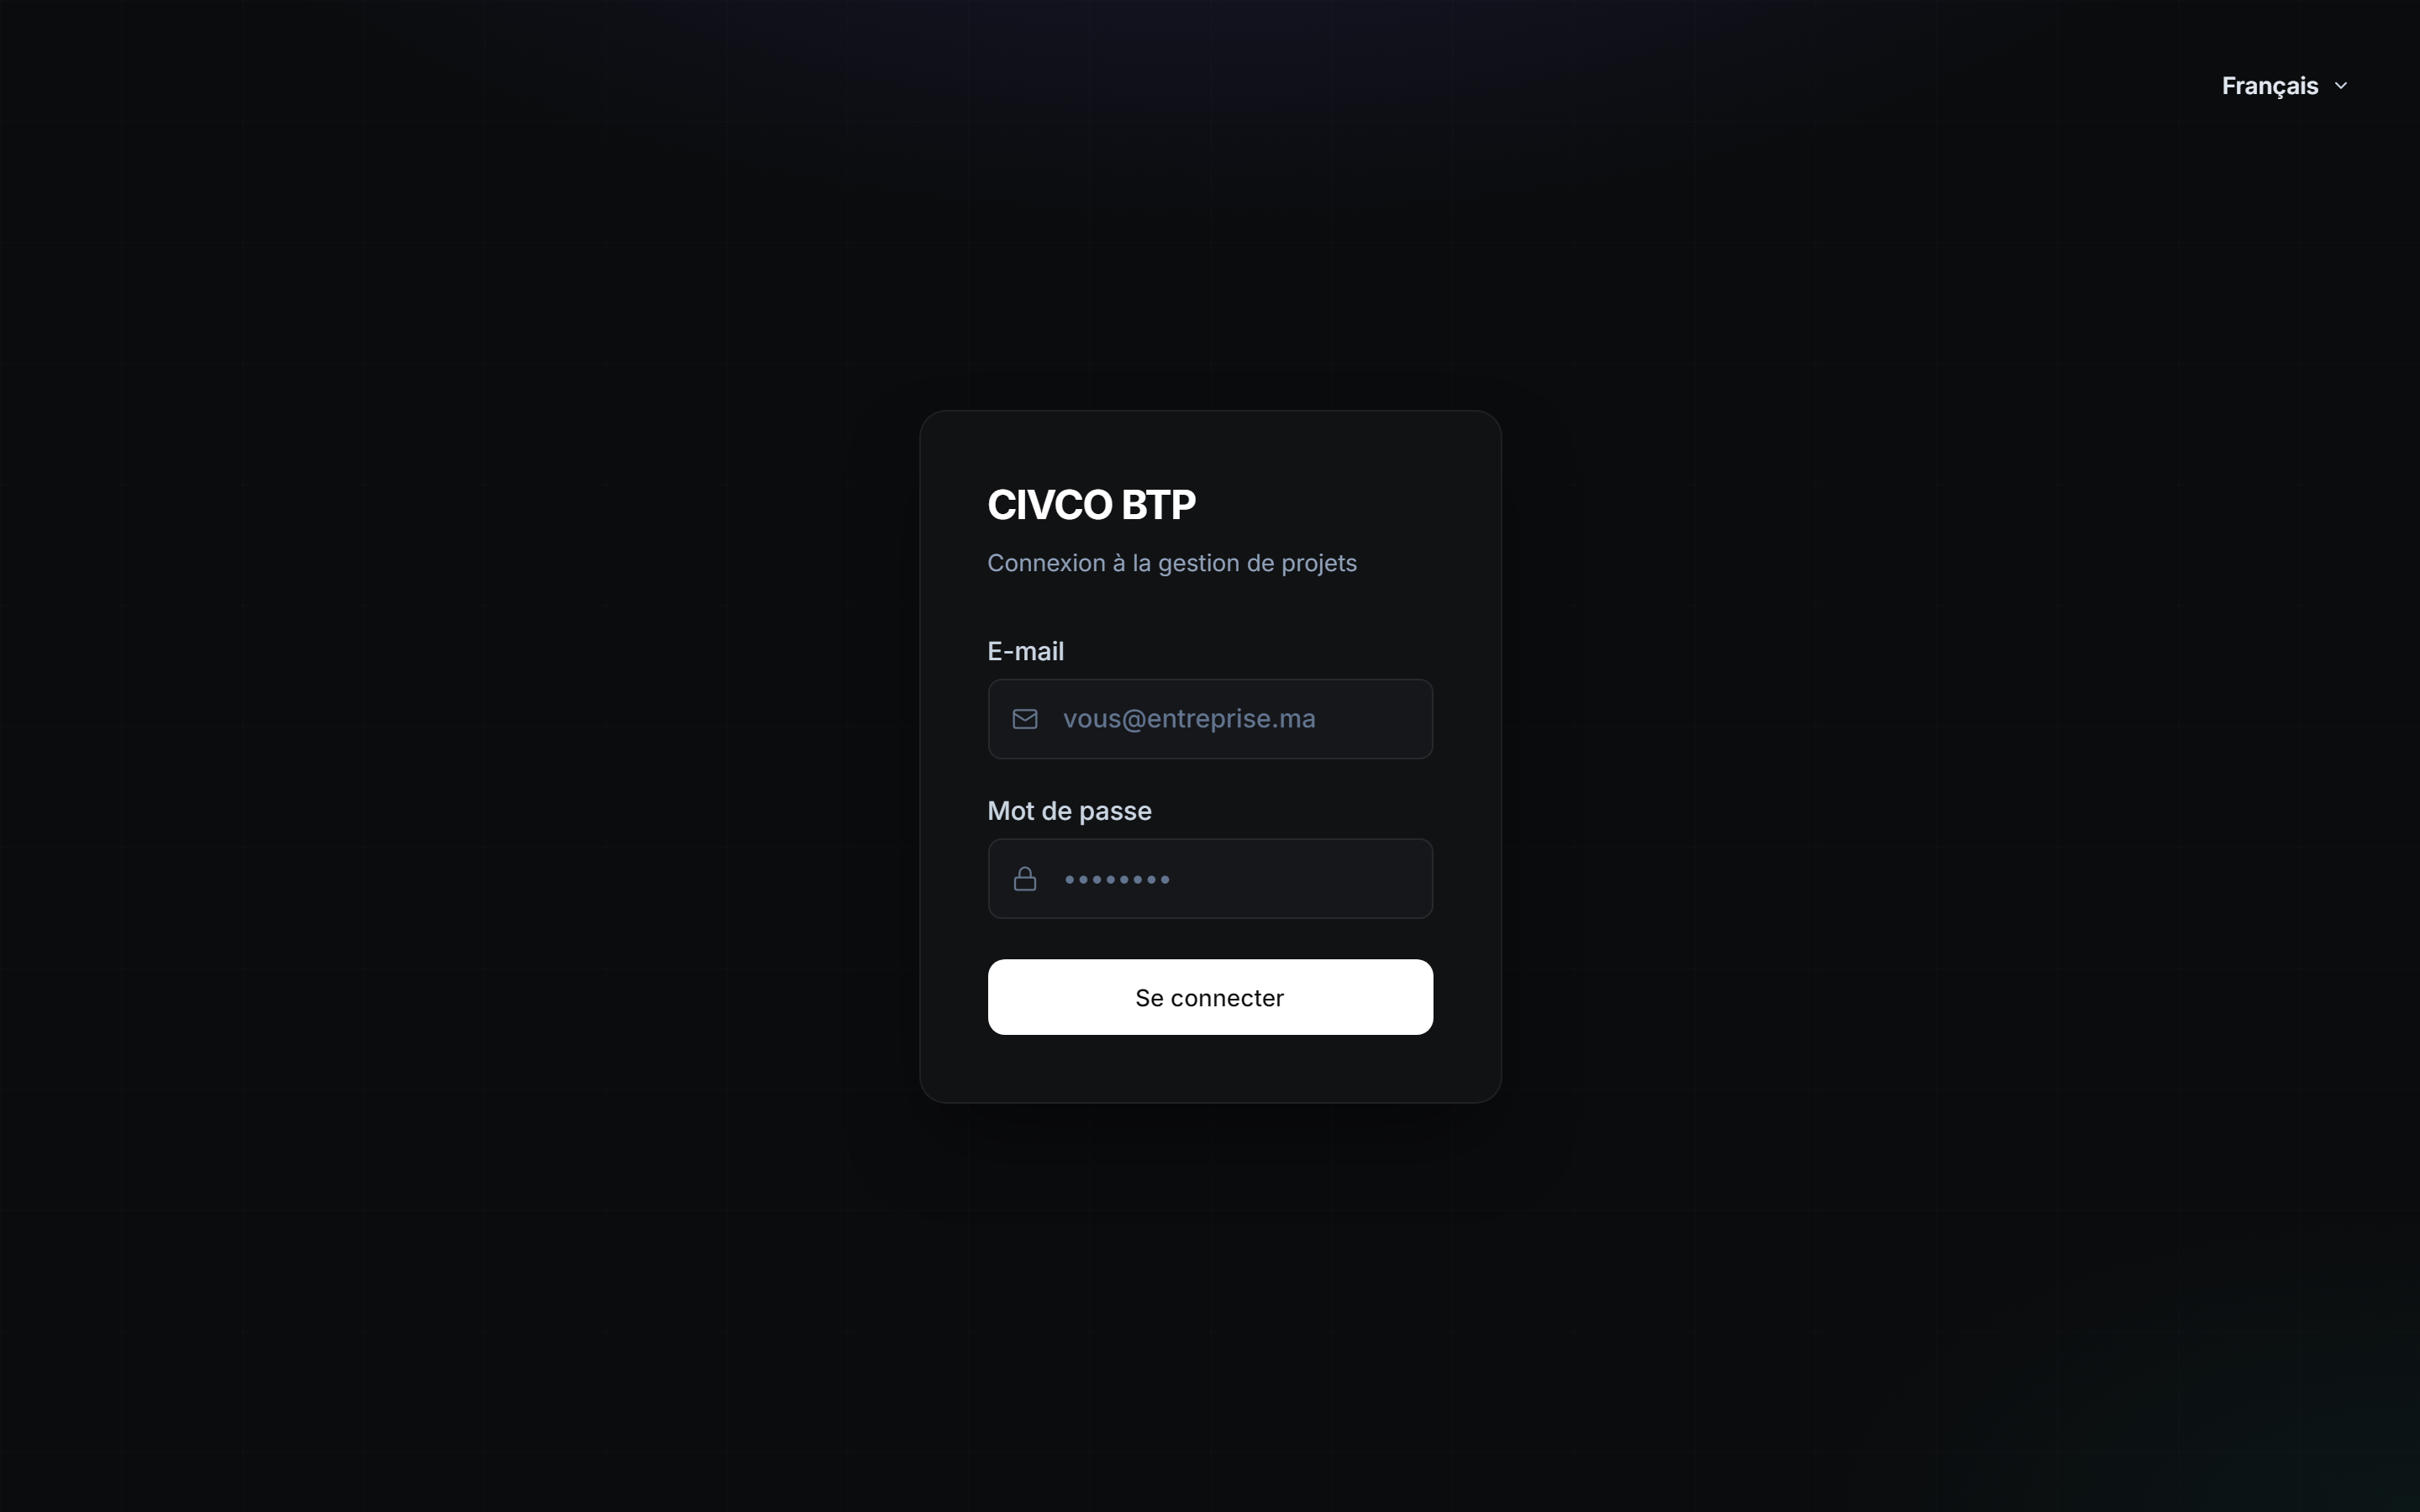
\includegraphics[width=\textwidth]{login.png}
  \caption{Page de connexion : authentification par email et mot de passe}
  \label{fig:login}
\end{figure}

La page de connexion (Figure~\ref{fig:login}) permet à tout utilisateur interne de
CIVCO BTP de s'authentifier. Après validation, l'utilisateur est redirigé vers la
page d'accueil correspondant à son profil métier.

\medskip

L'écran affiche le logo de l'entreprise, un formulaire email/mot de passe et une
option « Se souvenir de moi ». Les erreurs d'authentification (identifiants
incorrects, compte désactivé) sont affichées de manière explicite. Le design sombre
et épuré a été choisi pour réduire la fatigue visuelle lors d'une utilisation
quotidienne prolongée.

\subsection{Tableau de bord}

\begin{figure}[H]
  \centering
  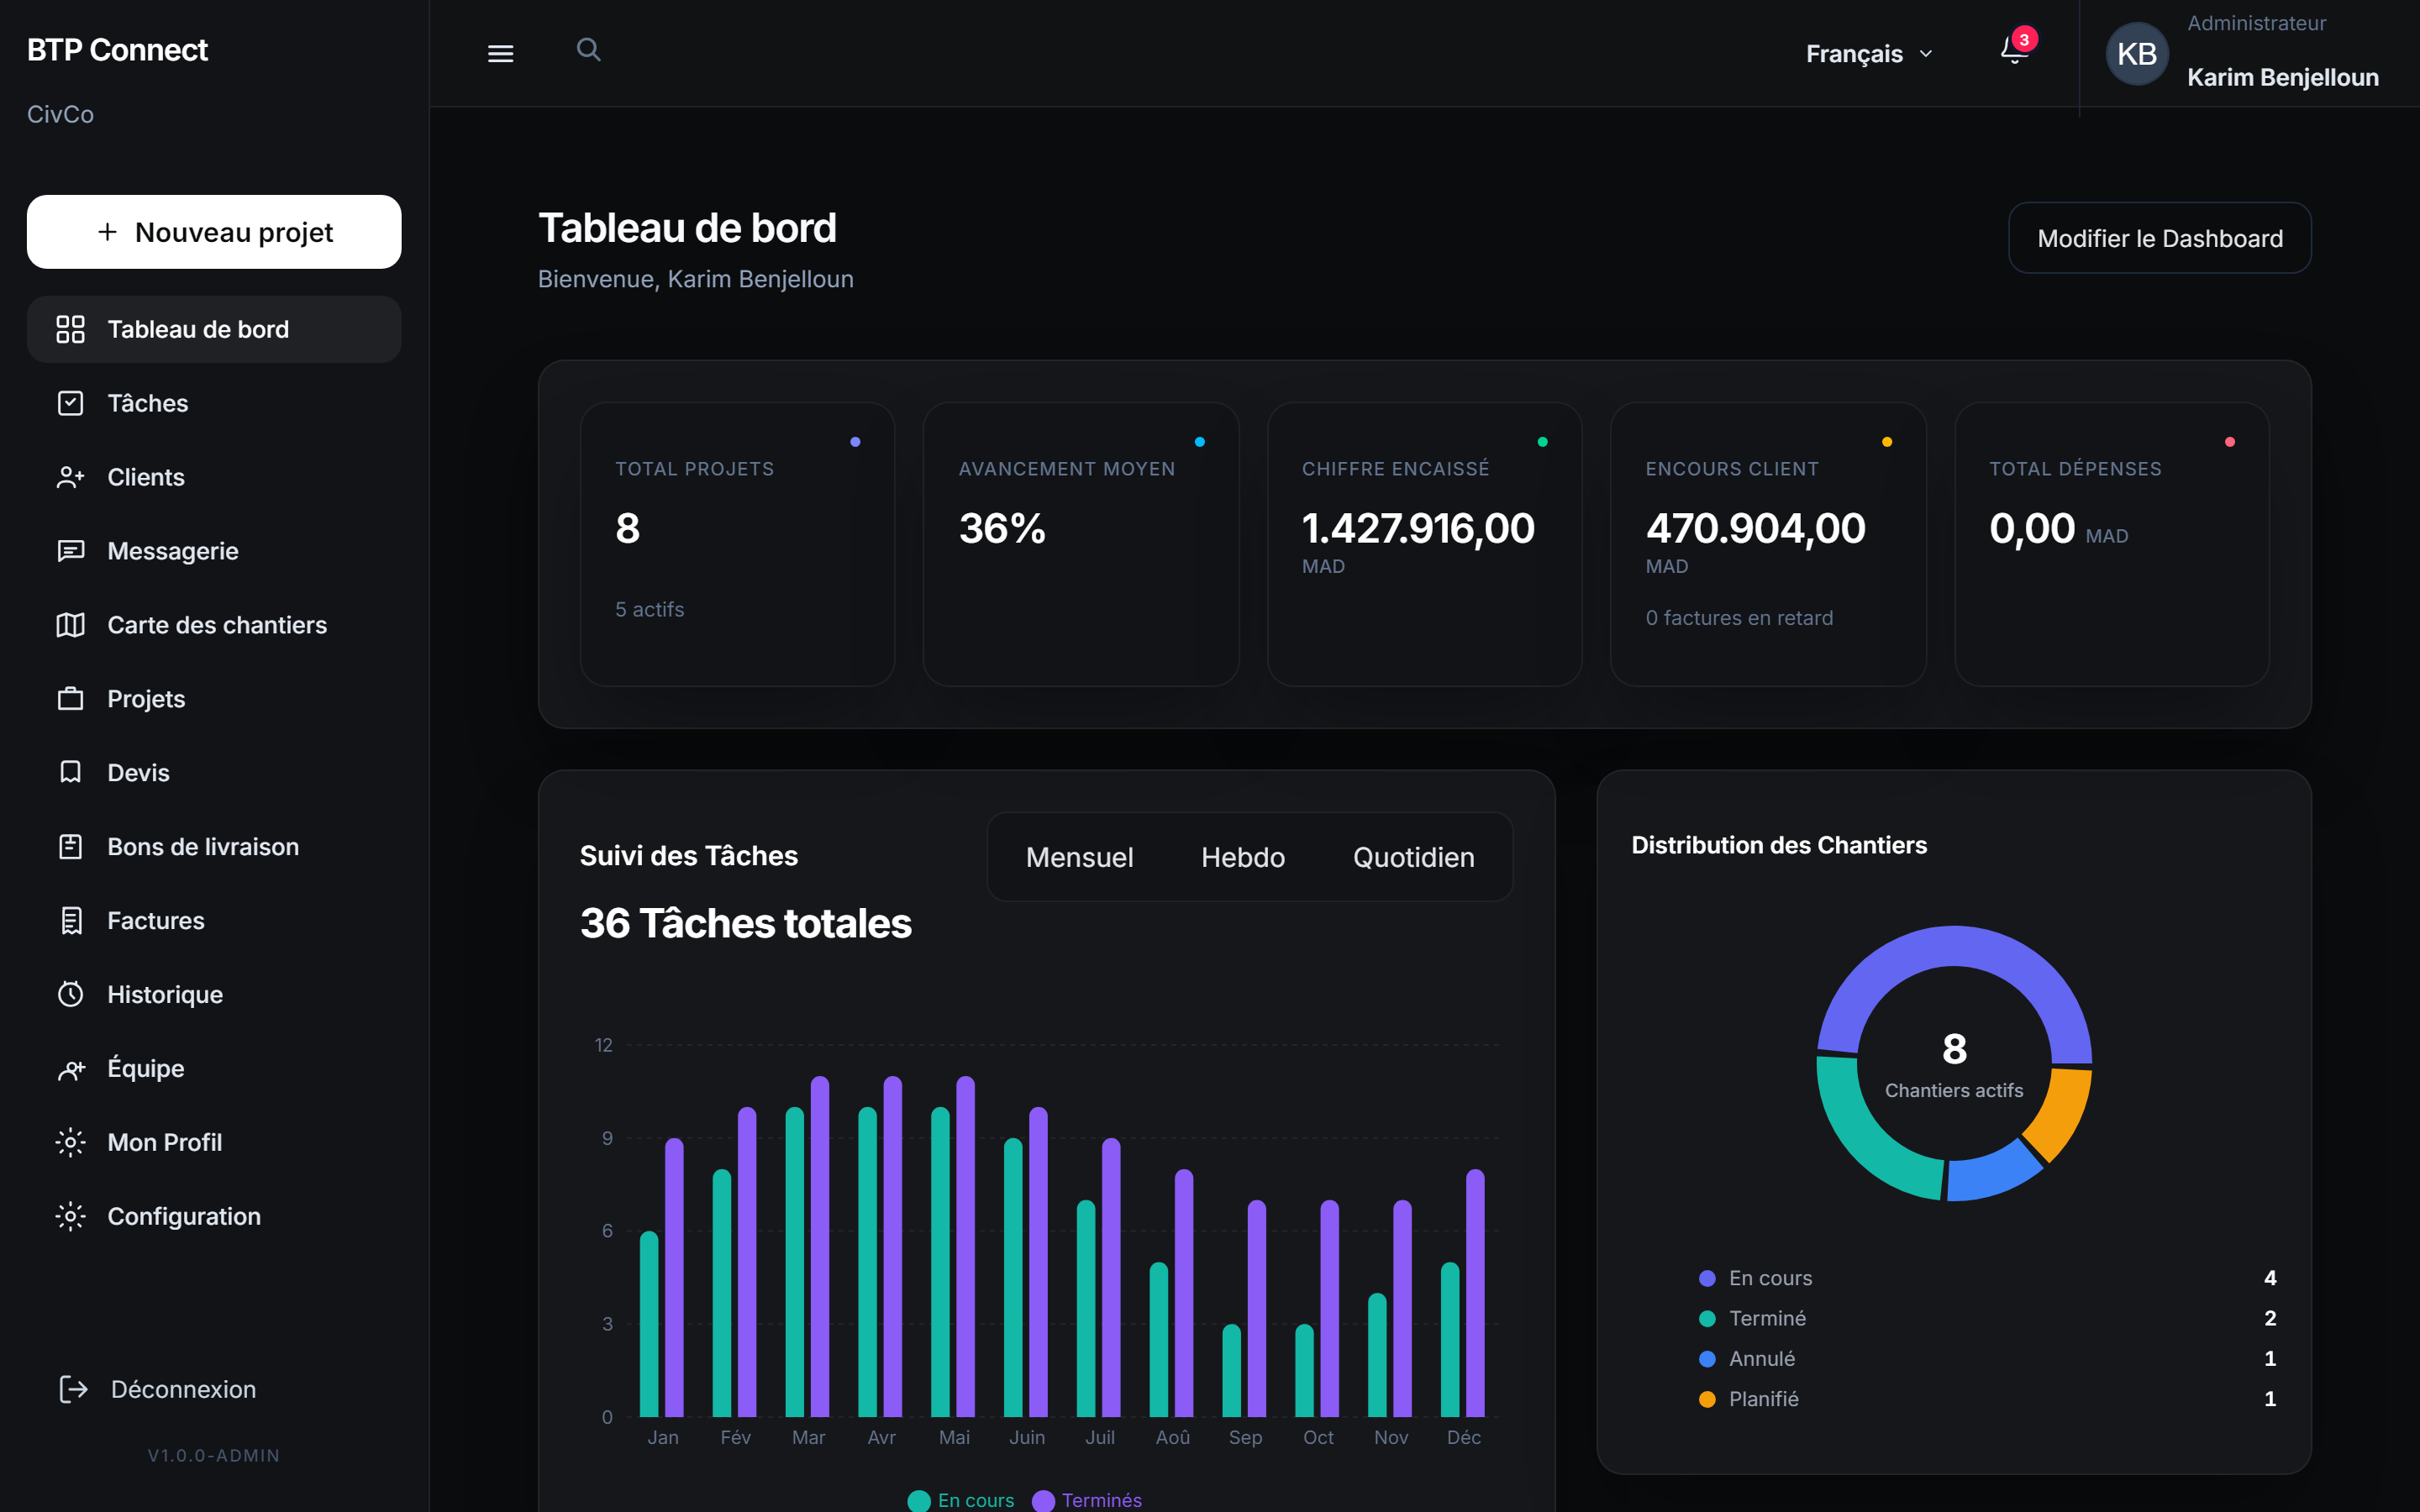
\includegraphics[width=\textwidth]{dashboard.png}
  \caption{Tableau de bord : vue synthétique de l'activité (projets, tâches, indicateurs)}
  \label{fig:dashboard}
\end{figure}

Le tableau de bord (Figure~\ref{fig:dashboard}) agrège les informations essentielles :
nombre de projets en cours, tâches prioritaires, graphiques d'avancement (Recharts)
et accès rapide aux modules. Les widgets affichés dépendent des permissions de
l'utilisateur connecté.

\medskip

Les widgets sont configurés dynamiquement : un administrateur voit l'ensemble des
indicateurs (projets actifs, factures en attente, tâches en retard), tandis qu'un
technicien ne voit que ses tâches assignées et les projets auxquels il participe.
Les graphiques Recharts illustrent l'évolution de l'avancement et la répartition
des projets par statut.

\subsection{Gestion des projets}

\begin{figure}[H]
  \centering
  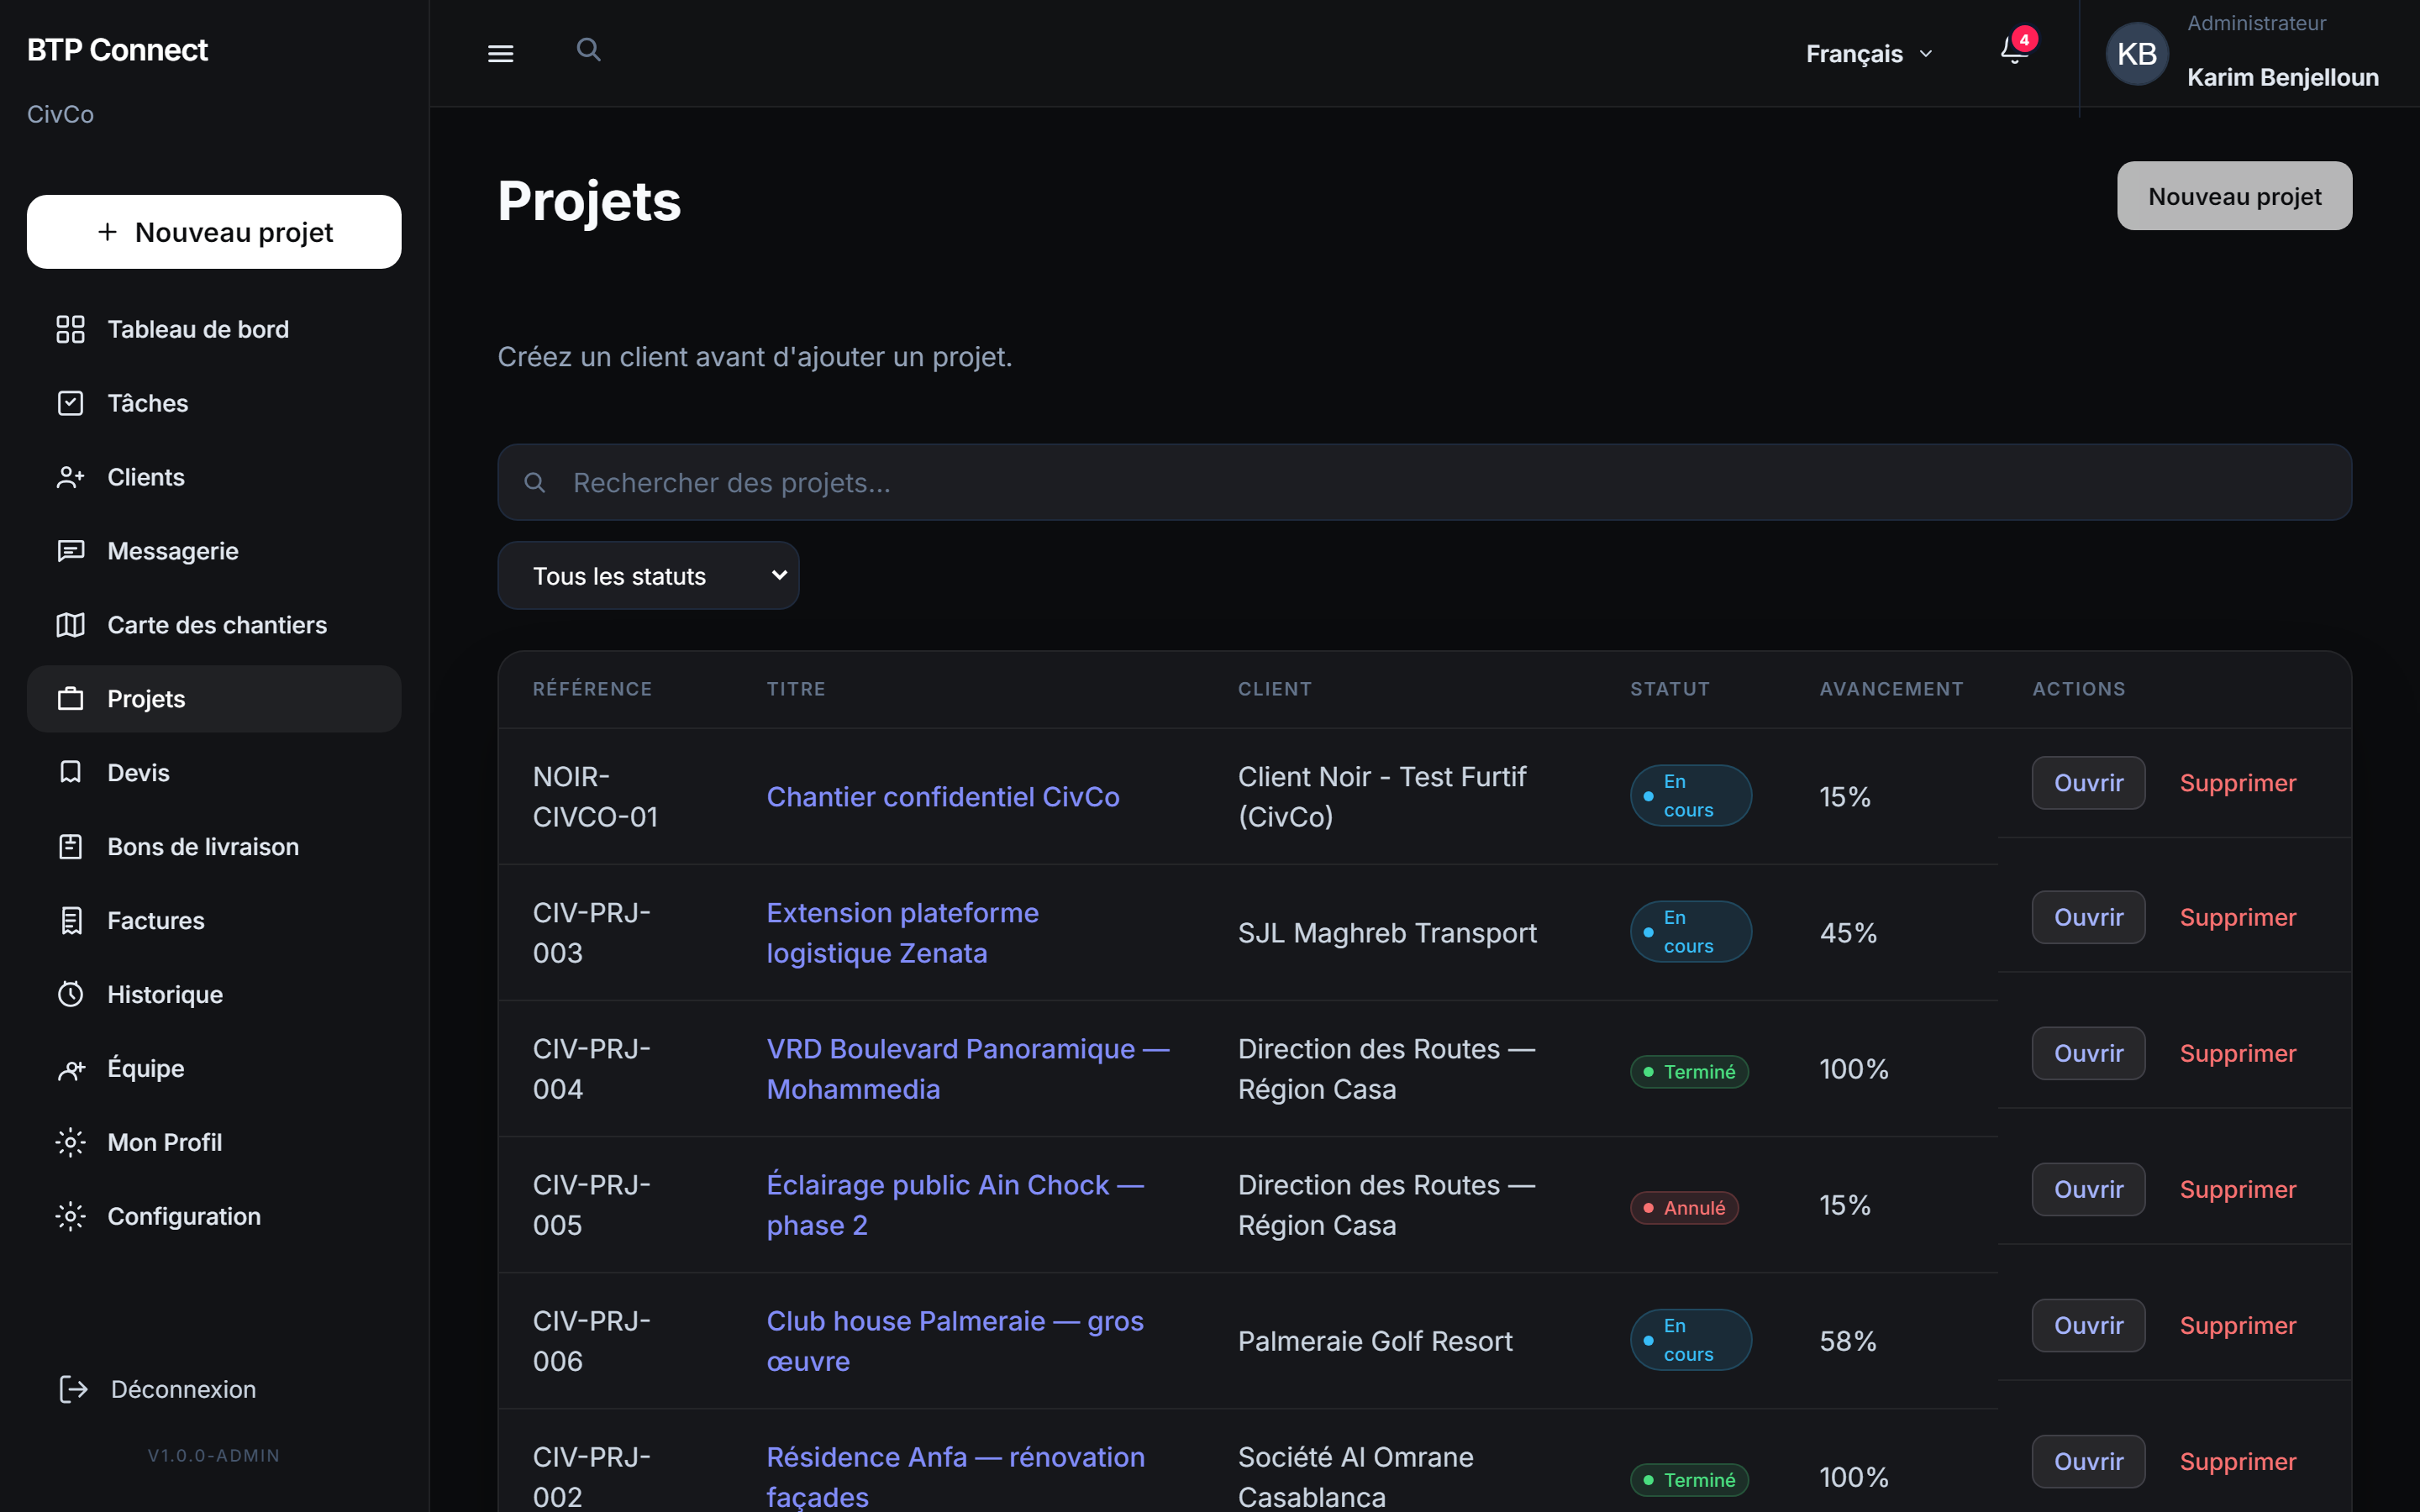
\includegraphics[width=\textwidth]{projects.png}
  \caption{Module Projets : liste des chantiers et fiche détail (phases, équipe, documents)}
  \label{fig:projects}
\end{figure}

Le module Projets (Figure~\ref{fig:projects}) permet de créer, consulter et modifier
les chantiers. La fiche détail est organisée en onglets : informations générales,
phases, tâches, équipe, devis/factures liés, contrats, dépenses et médias.

\medskip

La liste des projets propose des filtres par statut, client et nature de chantier.
La fiche détail centralise toutes les informations d'un chantier : depuis un seul
écran, le chef de projet peut consulter l'avancement des phases, réaffecter un
collaborateur, joindre un document ou créer un devis lié au projet.

\subsection{Gestion des clients}

\begin{figure}[H]
  \centering
  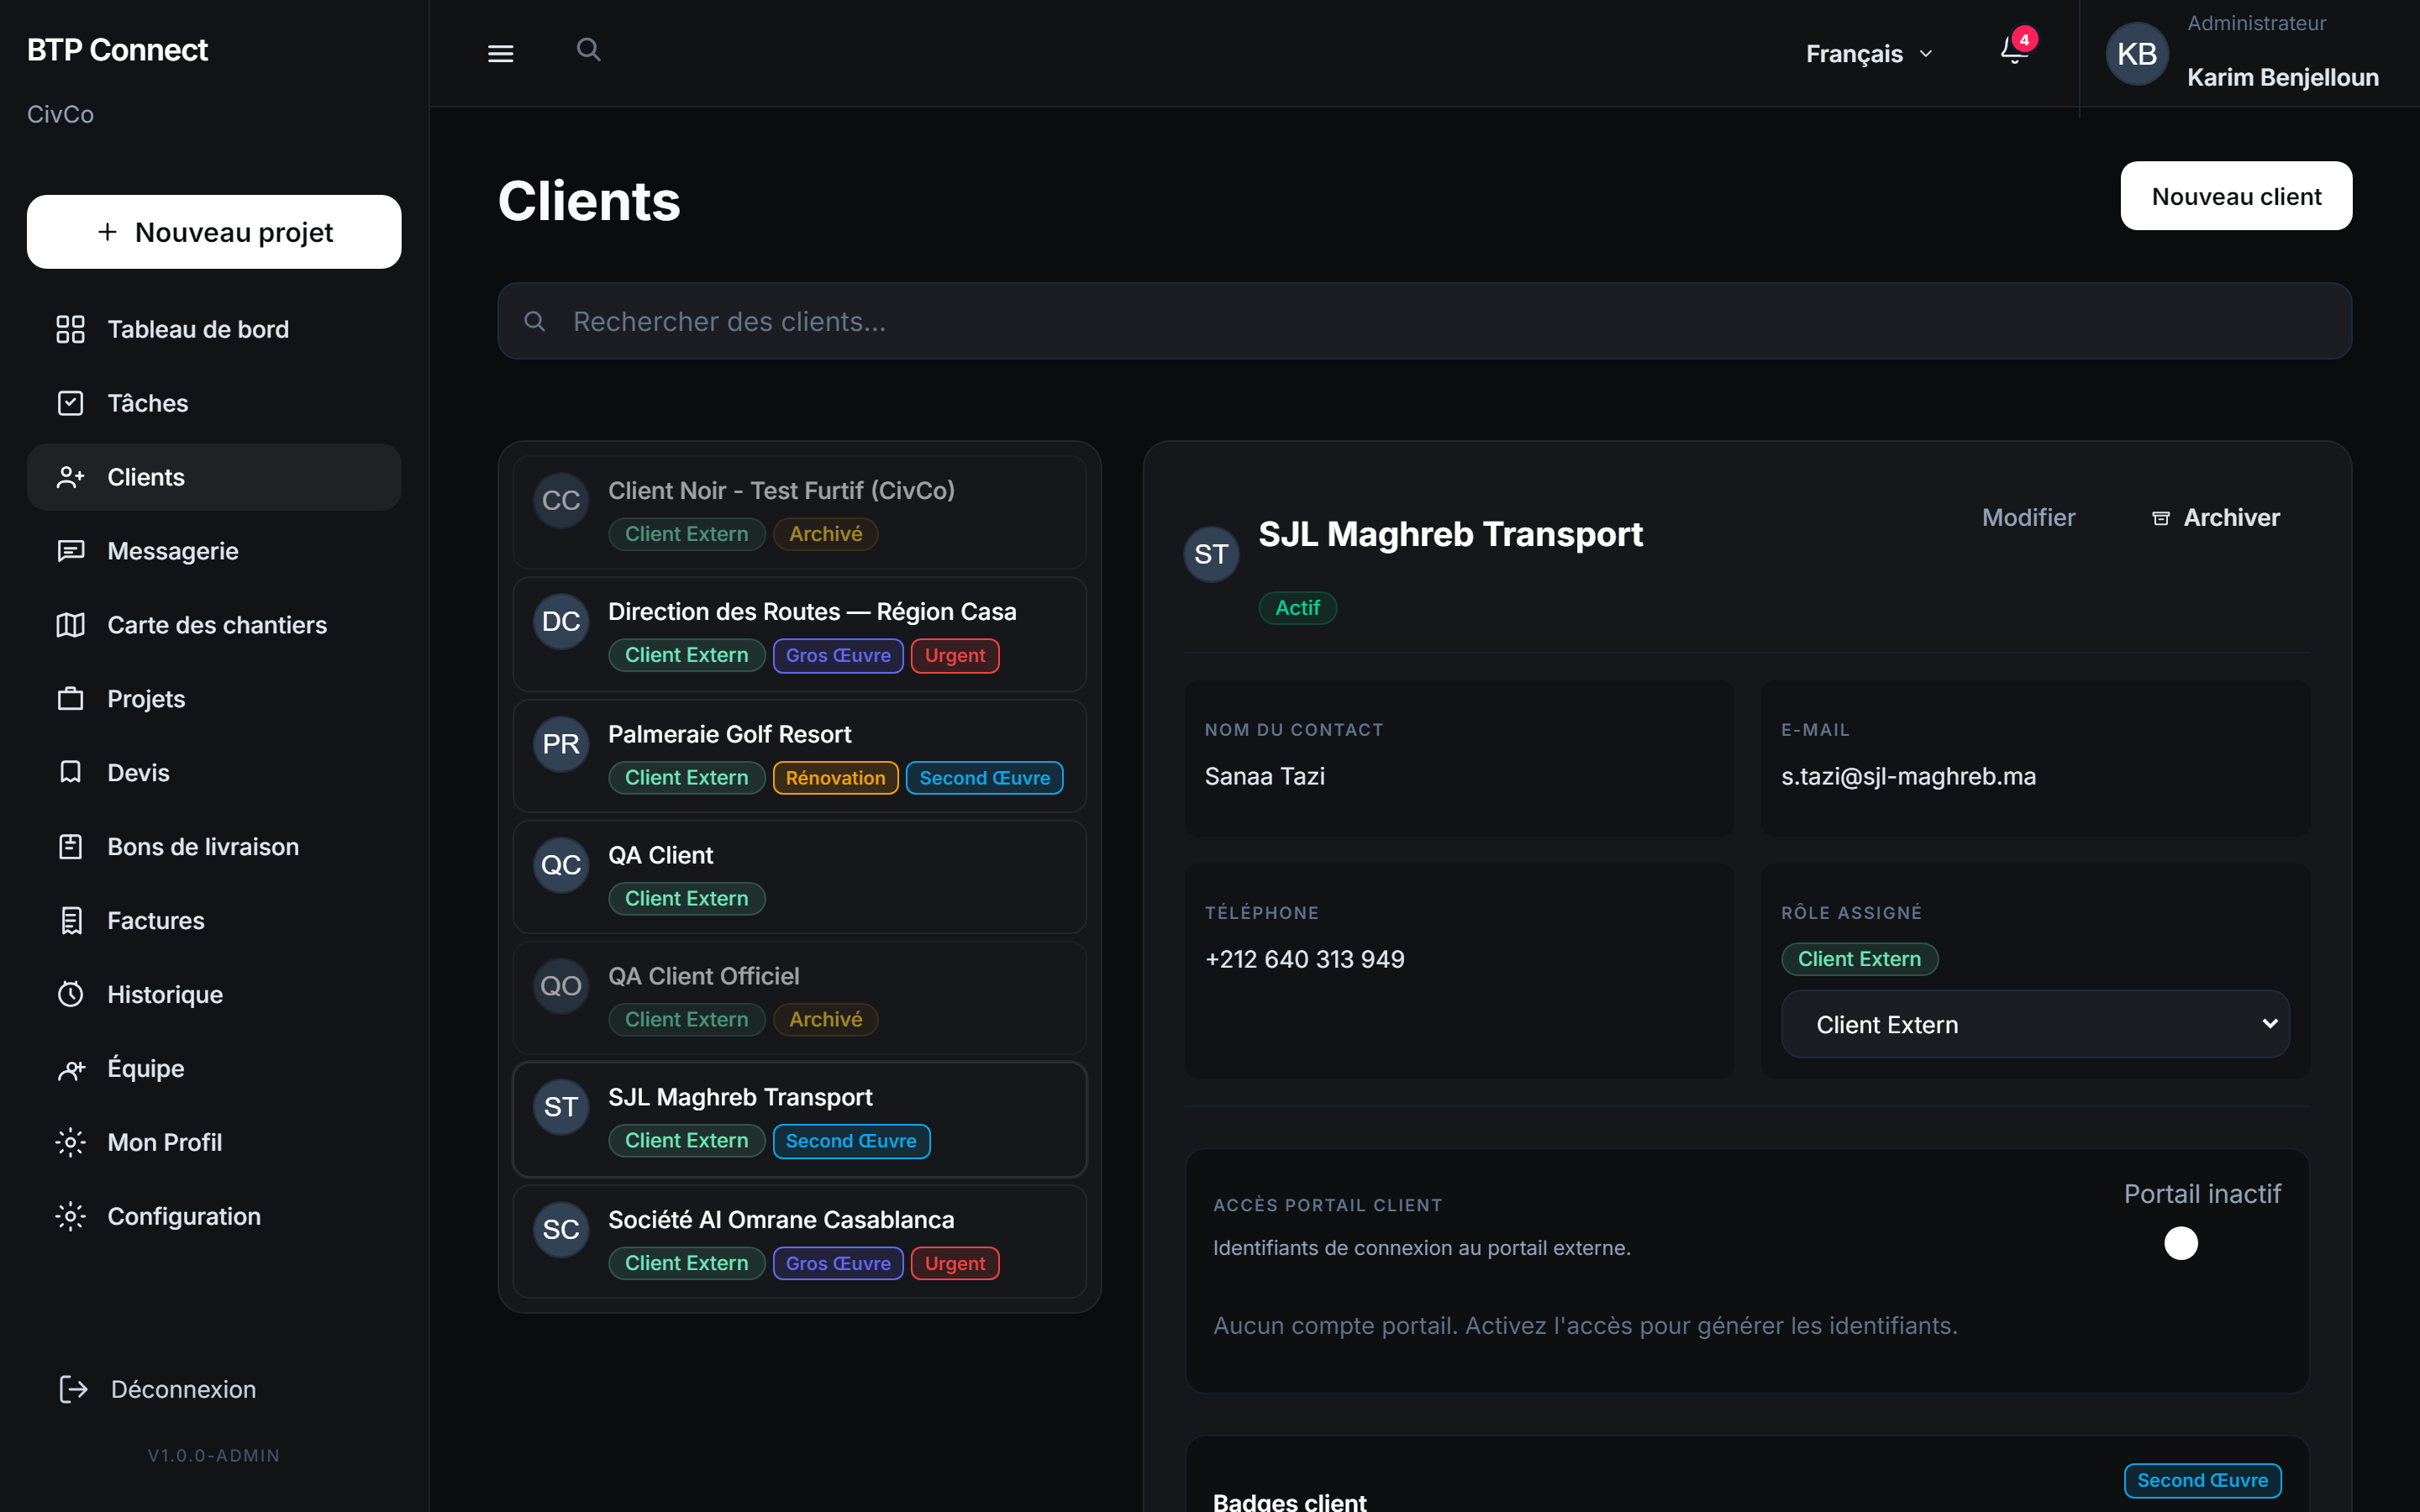
\includegraphics[width=\textwidth]{clients.png}
  \caption{Module Clients : fiches clients, contacts et archivage}
  \label{fig:clients}
\end{figure}

Le module Clients (Figure~\ref{fig:clients}) centralise les maîtres d'ouvrage et
clients commerciaux. L'administrateur peut provisionner un accès portail pour un
client externe directement depuis la fiche client.

\medskip

Chaque fiche client regroupe les coordonnées, les contacts associés, les badges
métier (Gros Œuvre, Urgent, etc.), l'historique des projets et l'état du compte
portail. L'archivage est sécurisé par une modale de confirmation pour éviter les
suppressions accidentelles.

\subsection{Documents commerciaux}

\begin{figure}[H]
  \centering
  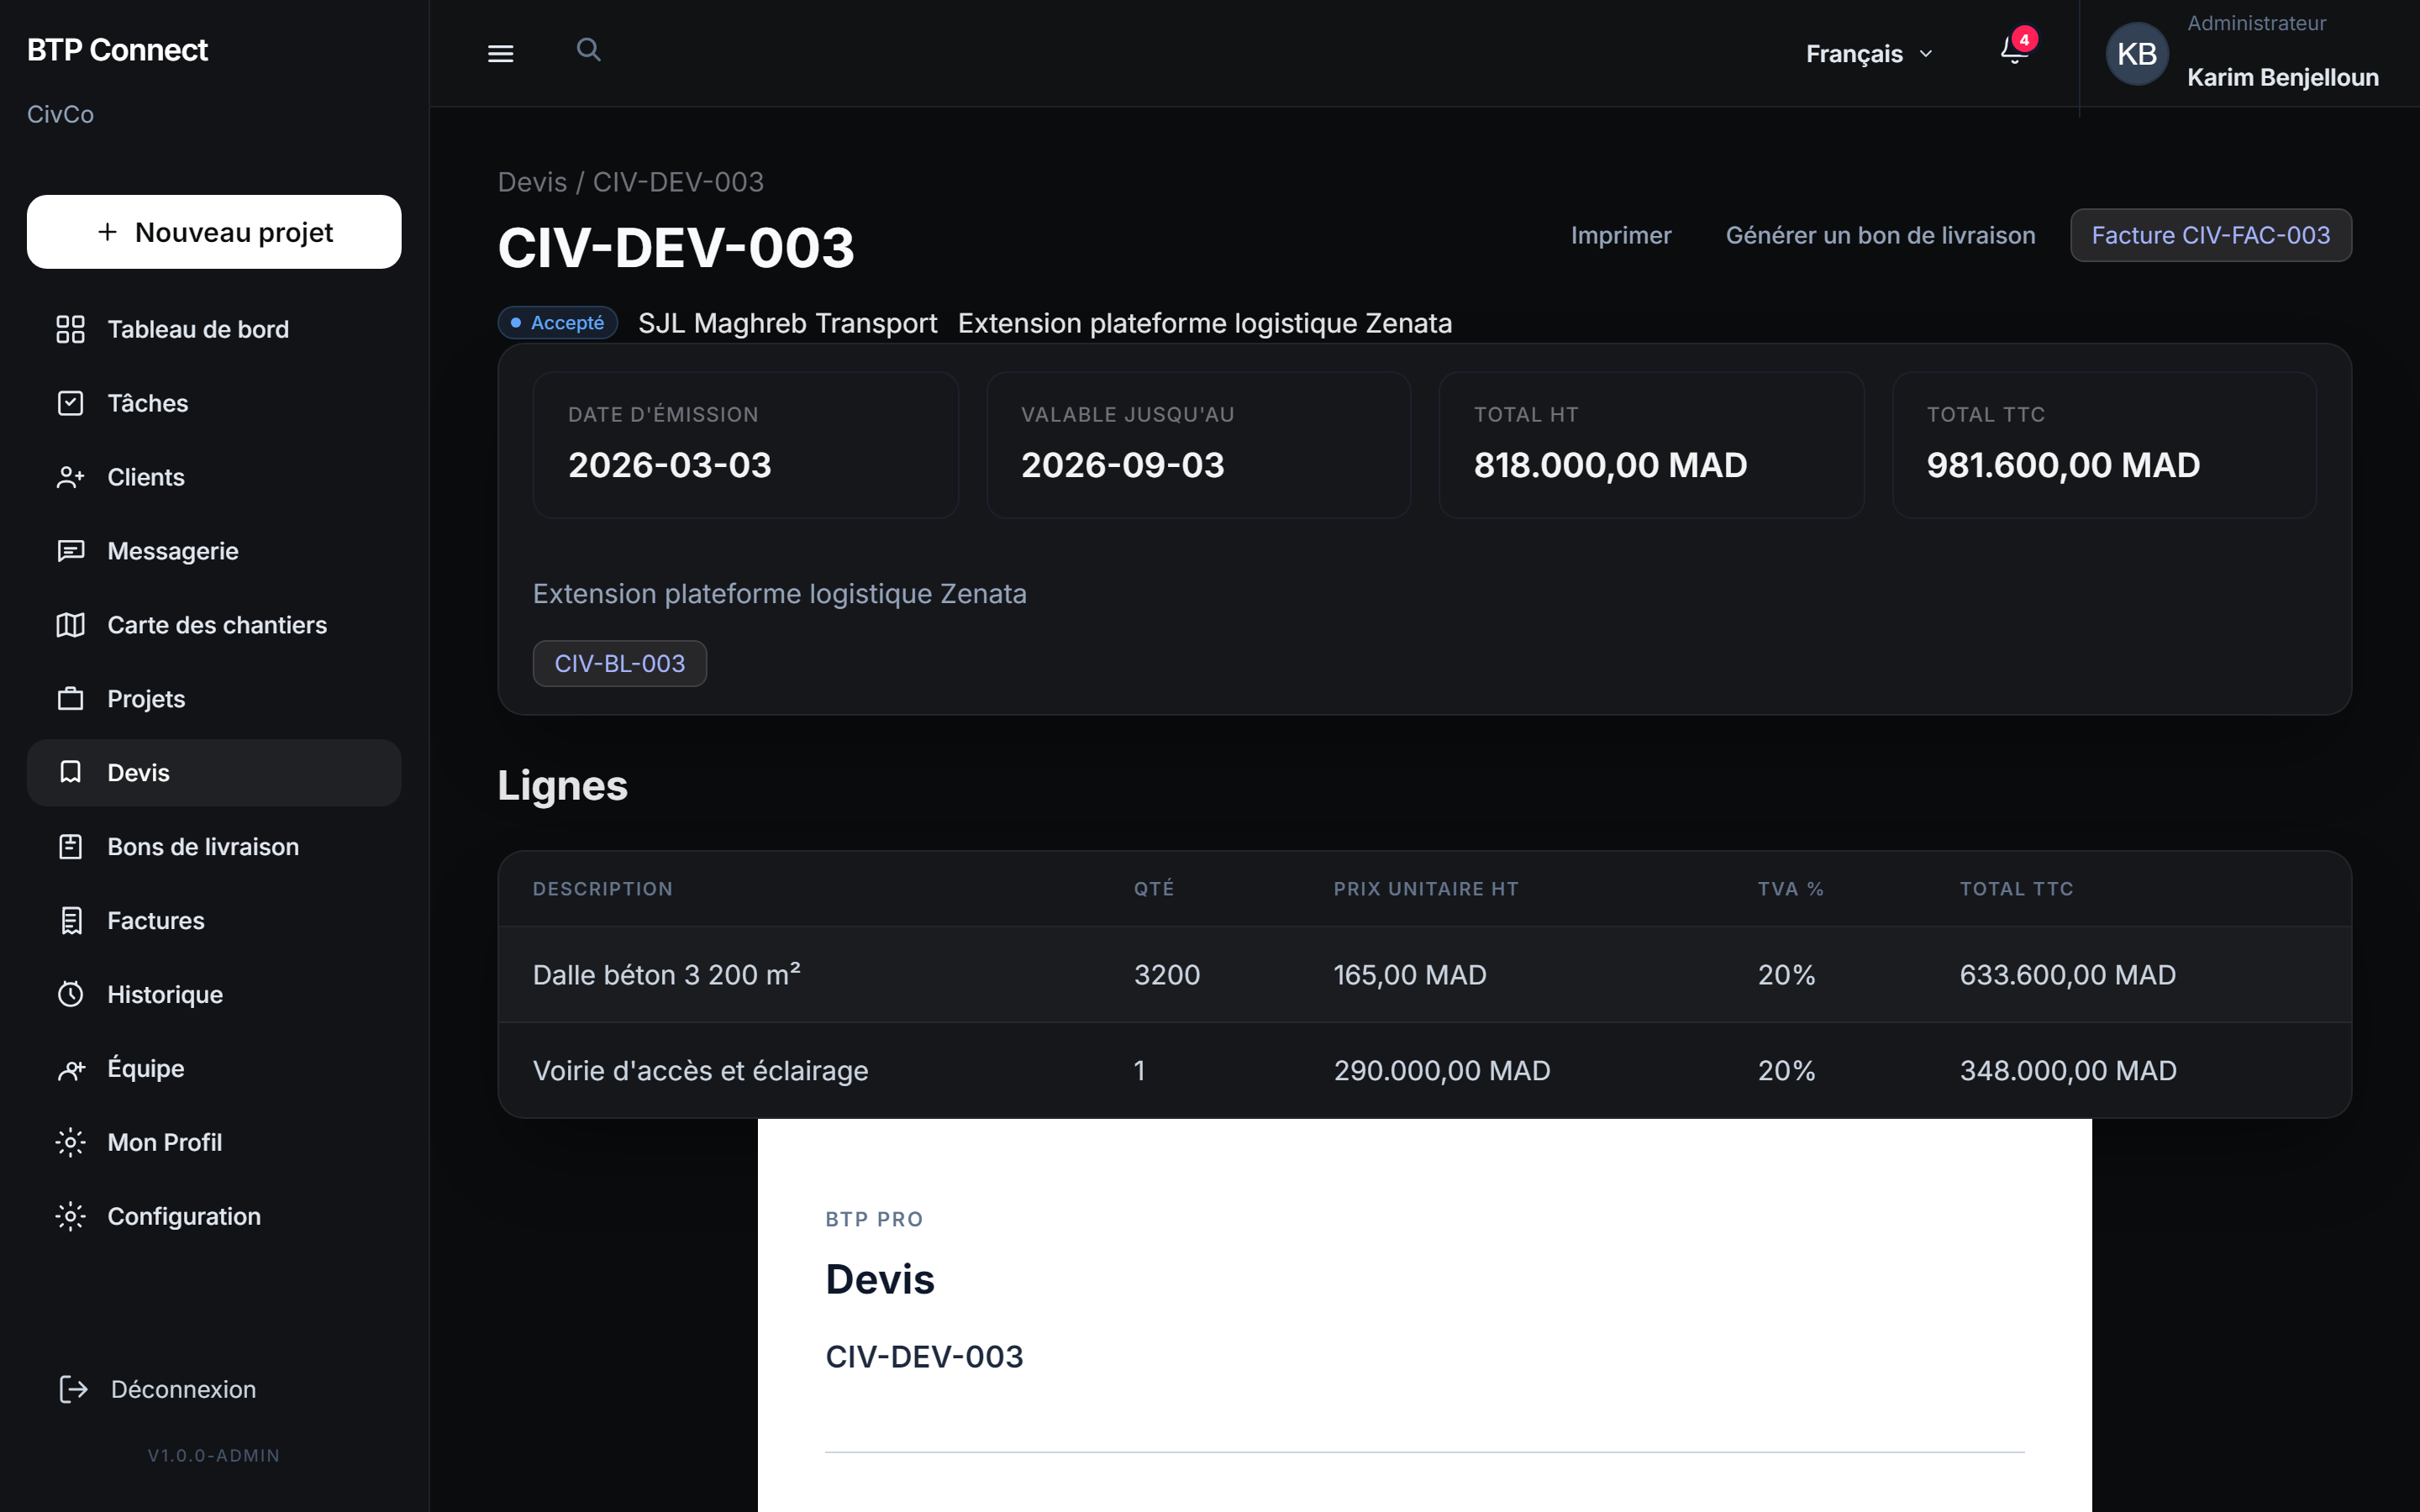
\includegraphics[width=\textwidth]{quotes.png}
  \caption{Module Devis : création avec lignes de détail et calcul automatique des totaux}
  \label{fig:quotes}
\end{figure}

\begin{figure}[H]
  \centering
  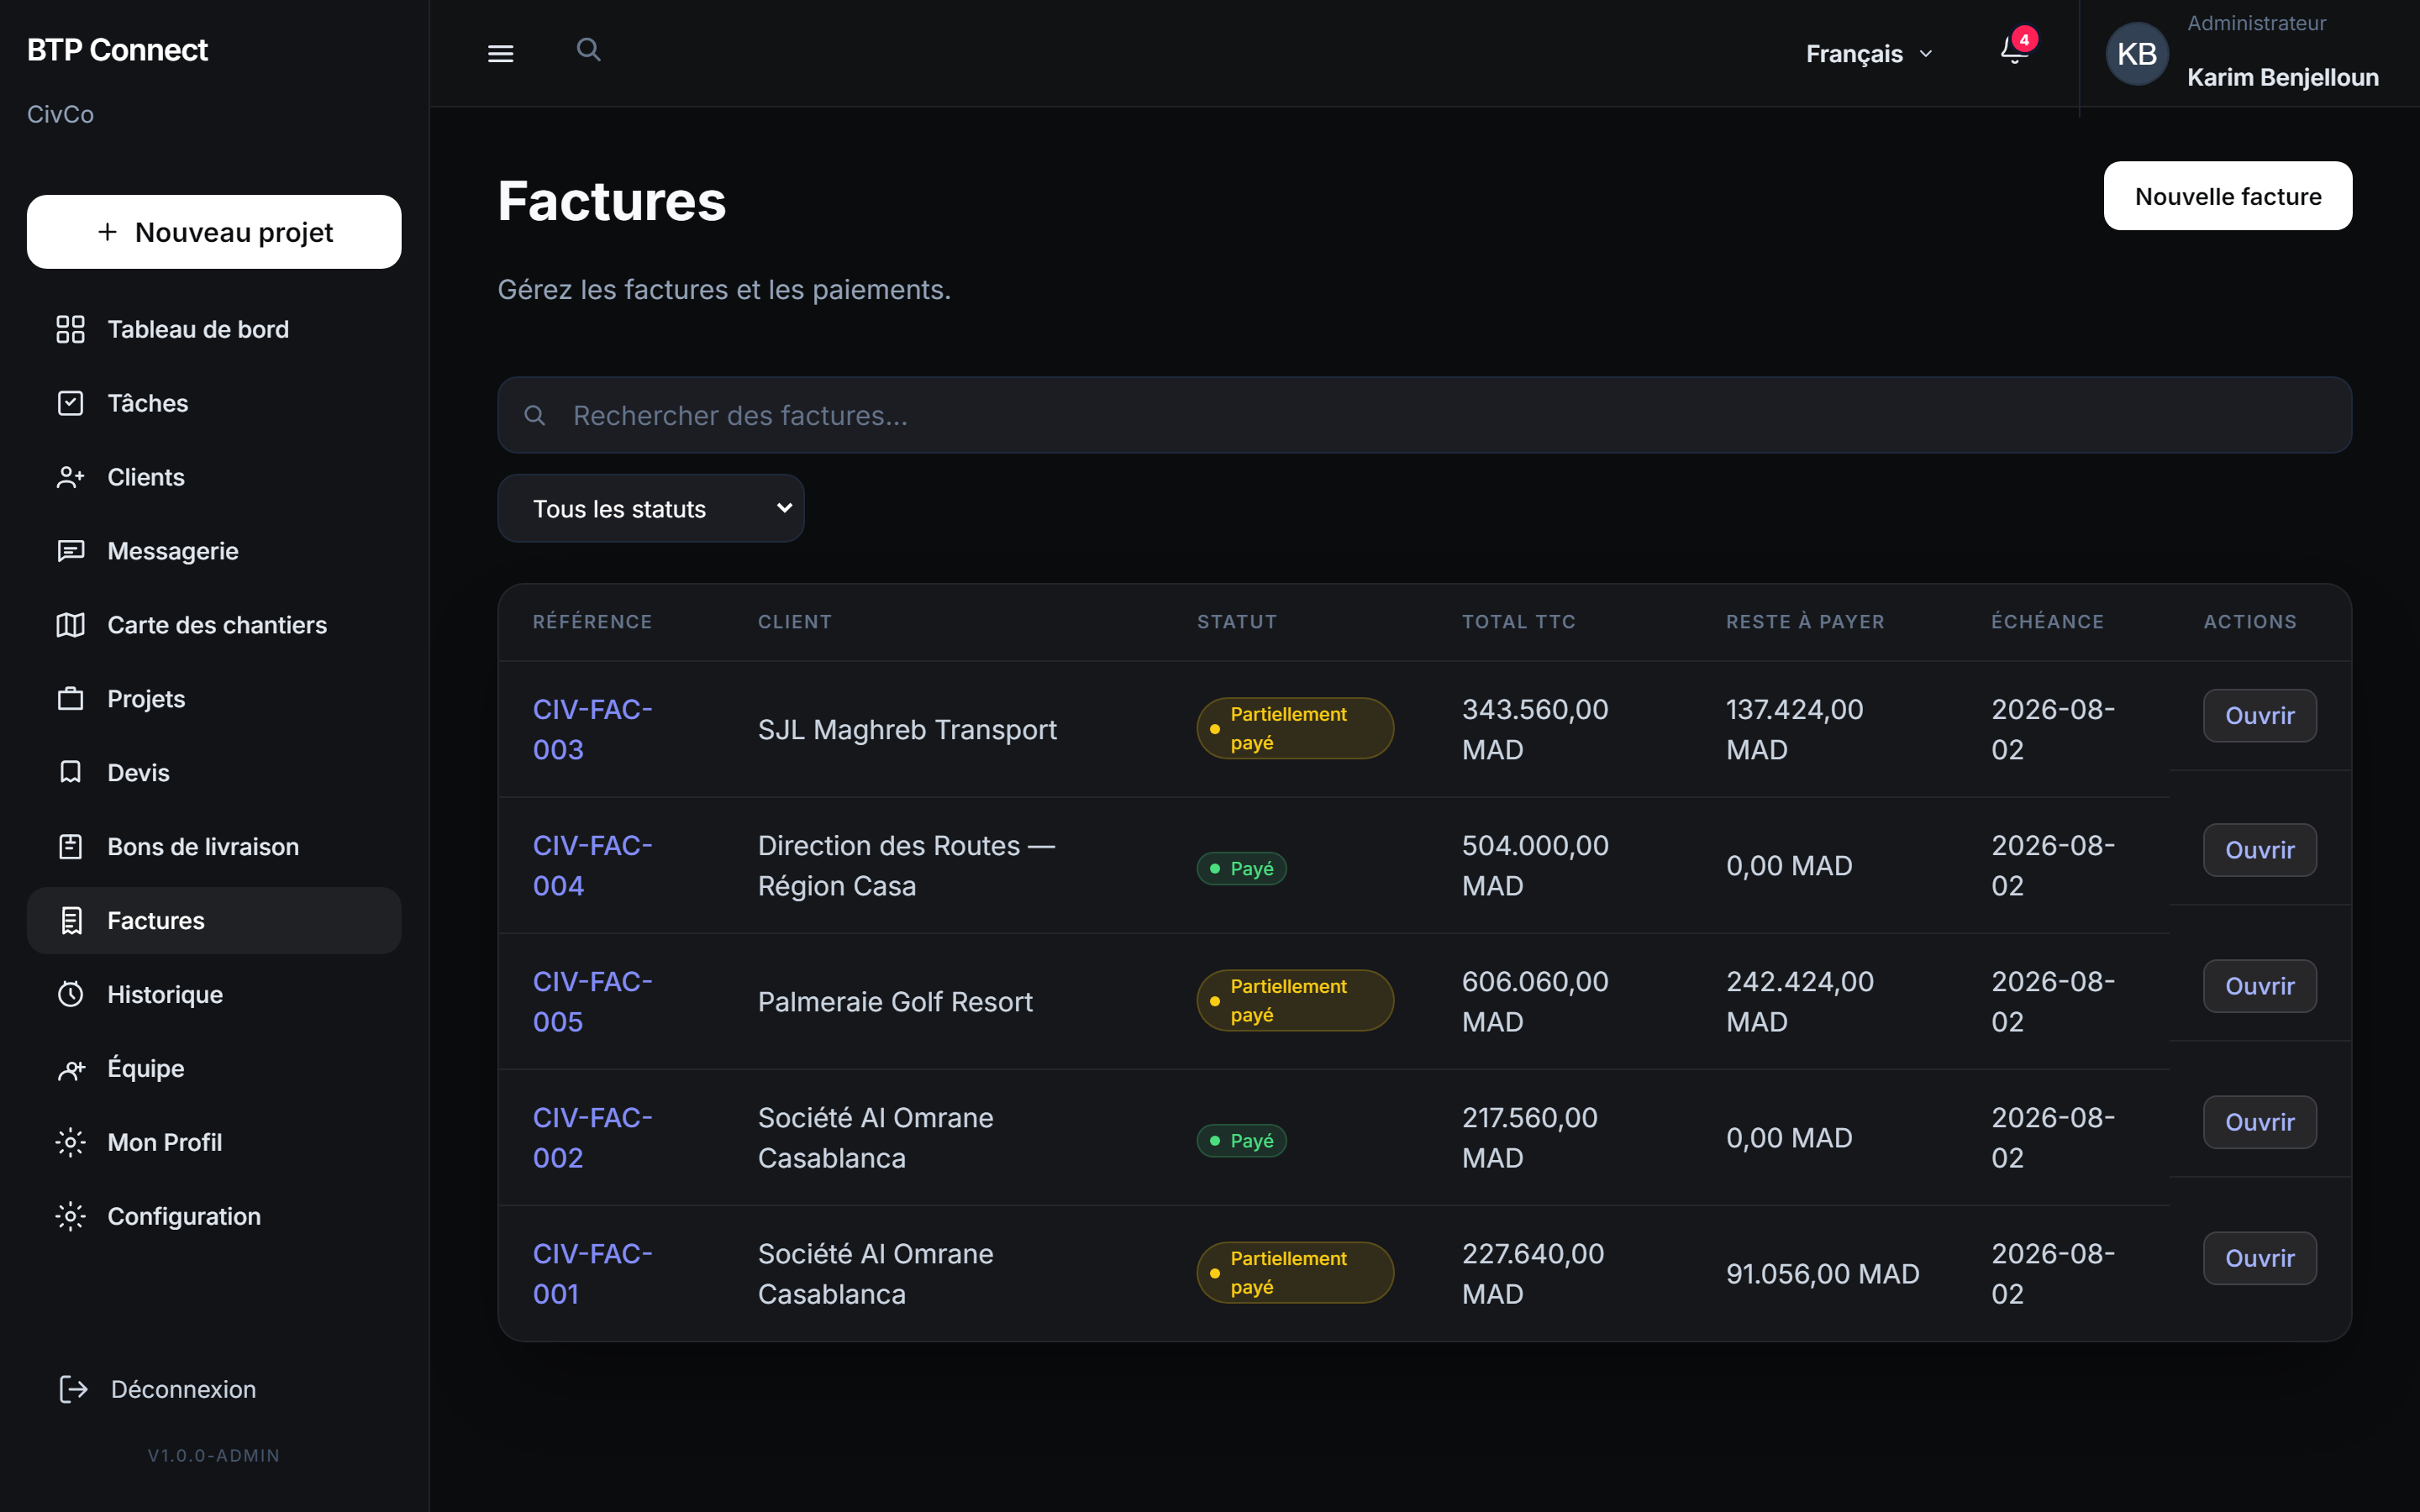
\includegraphics[width=\textwidth]{invoices.png}
  \caption{Module Factures : suivi des factures et état de paiement}
  \label{fig:invoices}
\end{figure}

Les modules Devis et Factures (Figures~\ref{fig:quotes} et~\ref{fig:invoices})
permettent la production des documents commerciaux, leur impression (avec suivi
des copies officielles) et la conversion devis $\rightarrow$ facture en un clic.

\medskip

Le formulaire de création de devis permet d'ajouter dynamiquement des lignes de
prestation (description, quantité, prix unitaire HT, taux de TVA). Les totaux sont
recalculés en temps réel. L'impression s'effectue via un composant React dédié
(\texttt{CommercialPrintSheet}) qui génère une version formatée prête à l'envoi au
client, avec suivi du quota d'impressions officielles.

\subsection{Planification des tâches}

\begin{figure}[H]
  \centering
  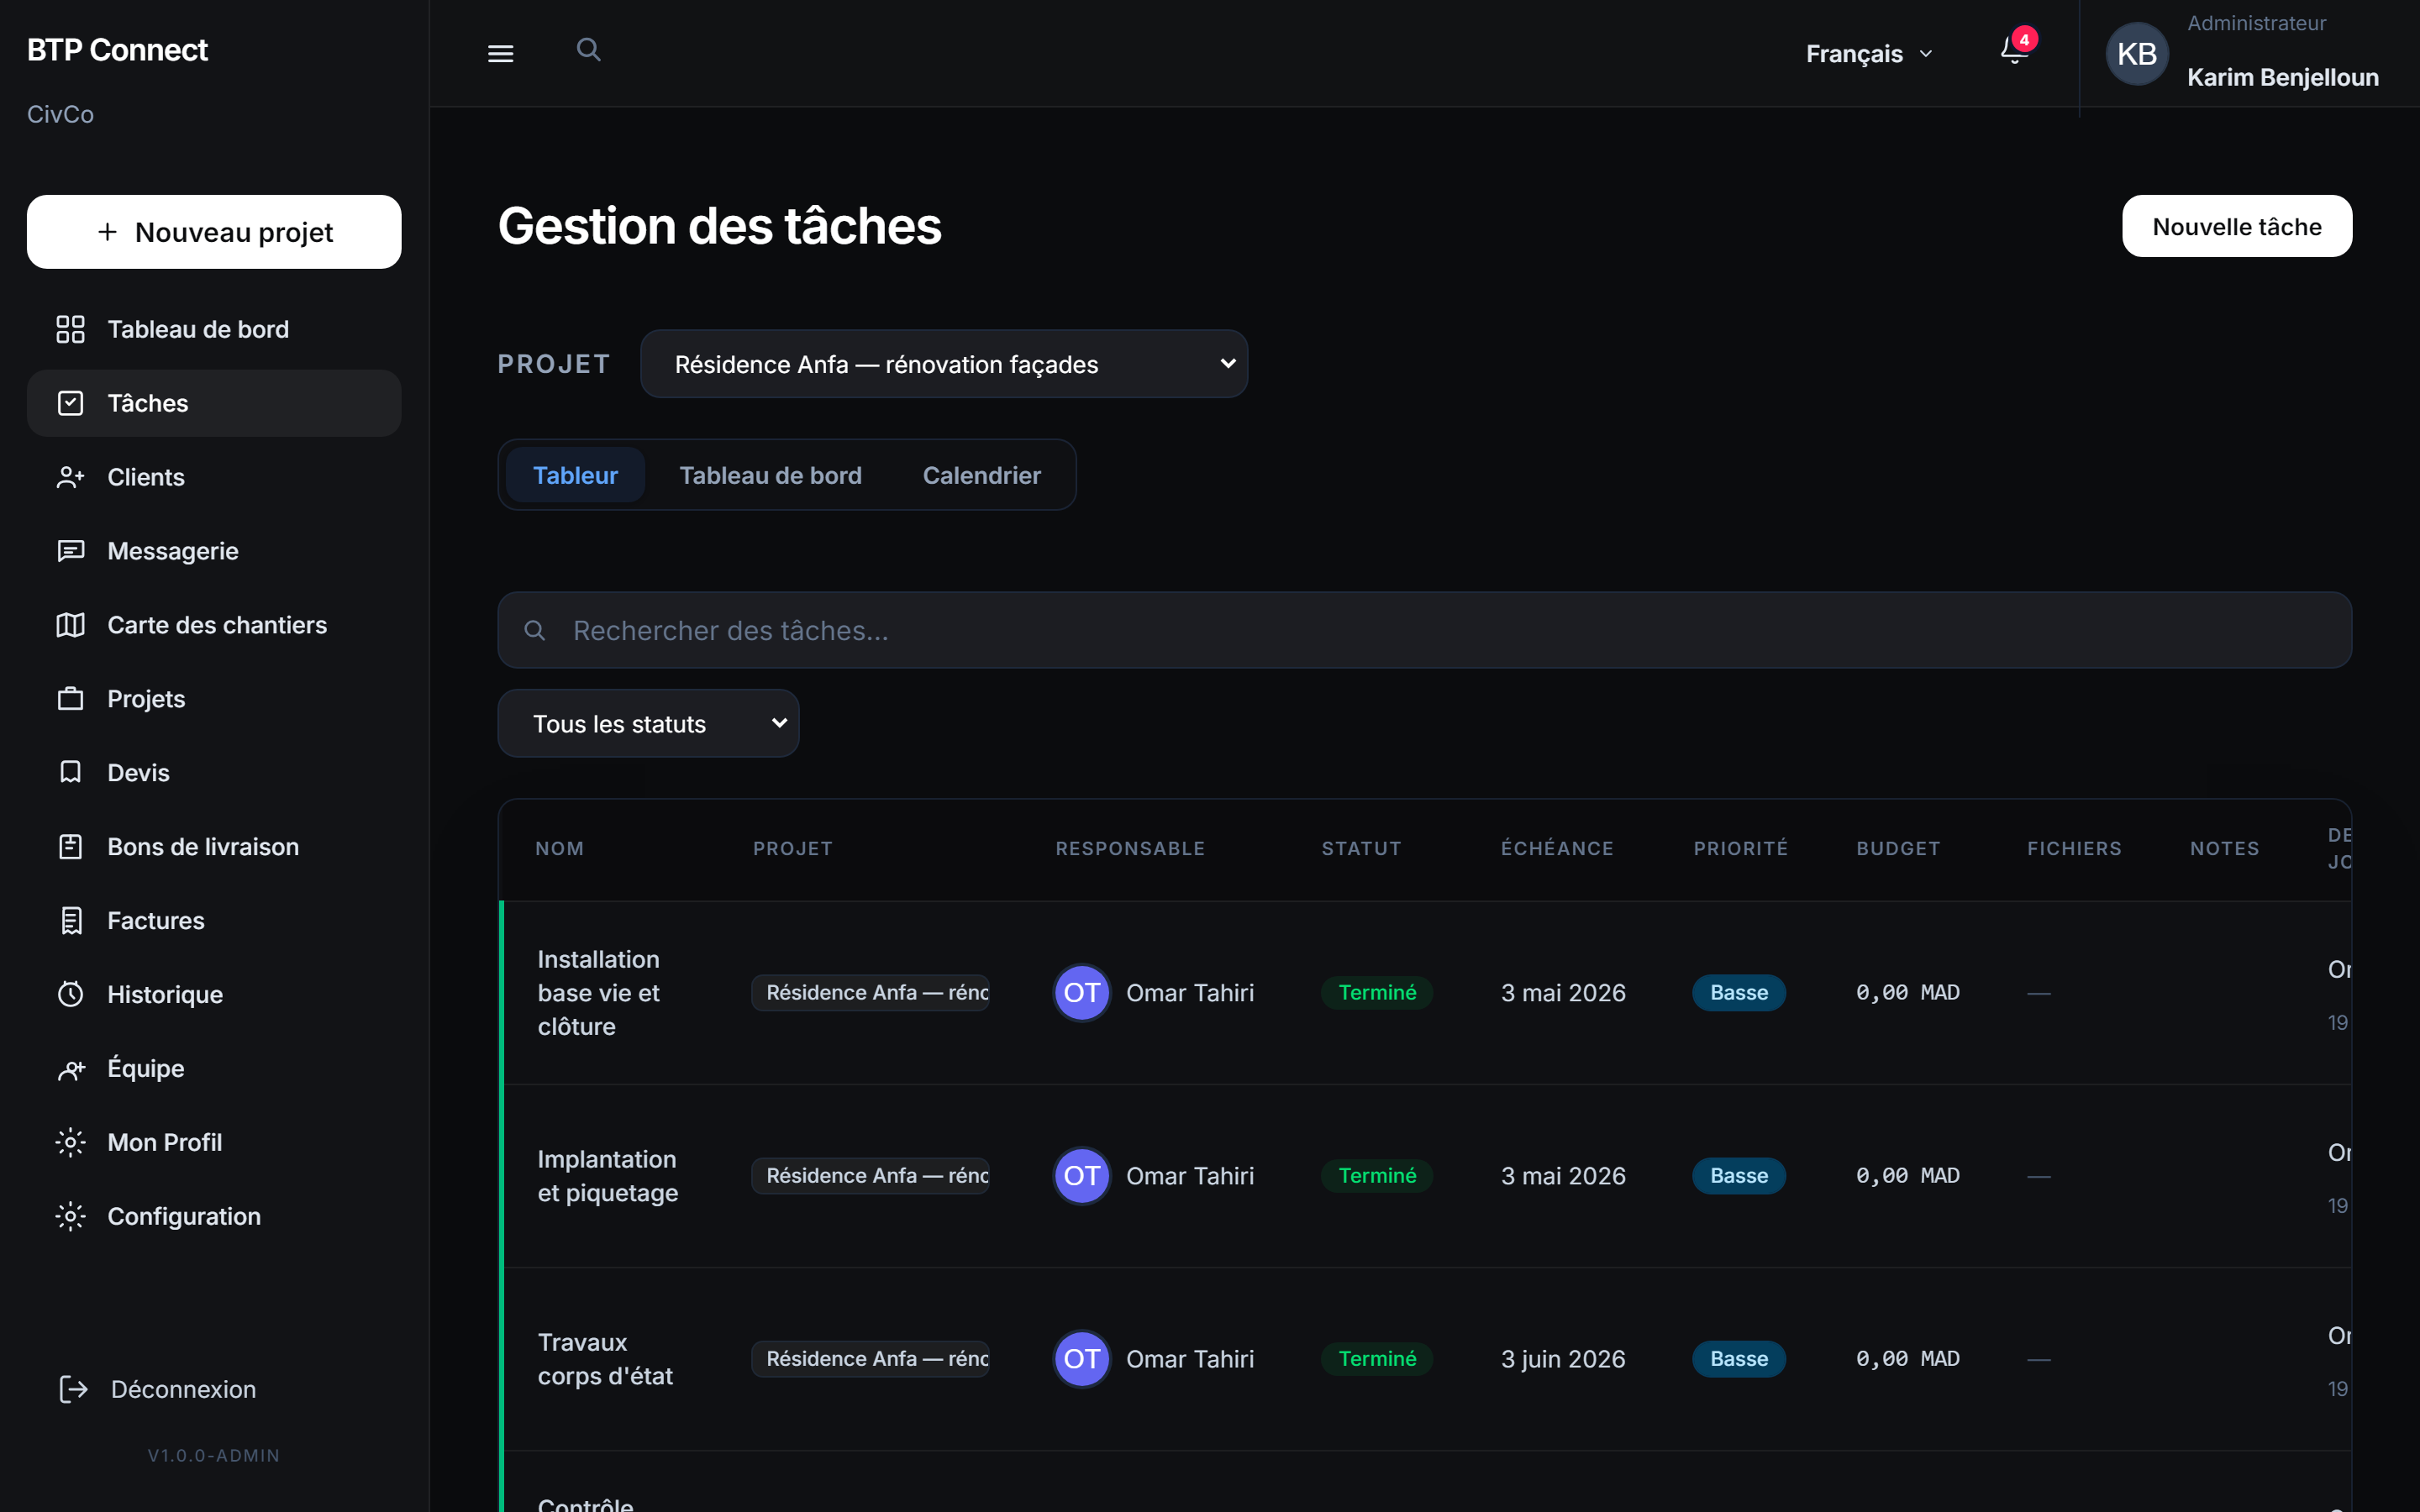
\includegraphics[width=\textwidth]{tasks.png}
  \caption{Module Tâches : planification, assignation et suivi par projet}
  \label{fig:tasks}
\end{figure}

Le module Tâches (Figure~\ref{fig:tasks}) offre une vue tableau des missions
opérationnelles, filtrable par statut, projet et assigné. Les chefs de projet
peuvent créer et assigner des tâches ; les utilisateurs internes consultent
leurs tâches propres.

\medskip

Le module propose une vue tableau avec tri par date d'échéance, filtre par statut
(à faire, en cours, terminé) et code couleur pour les tâches en retard. La création
d'une tâche associe obligatoirement un projet, une phase et un responsable, garantissant
la traçabilité de l'assignation.

\subsection{Carte des chantiers}

\begin{figure}[H]
  \centering
  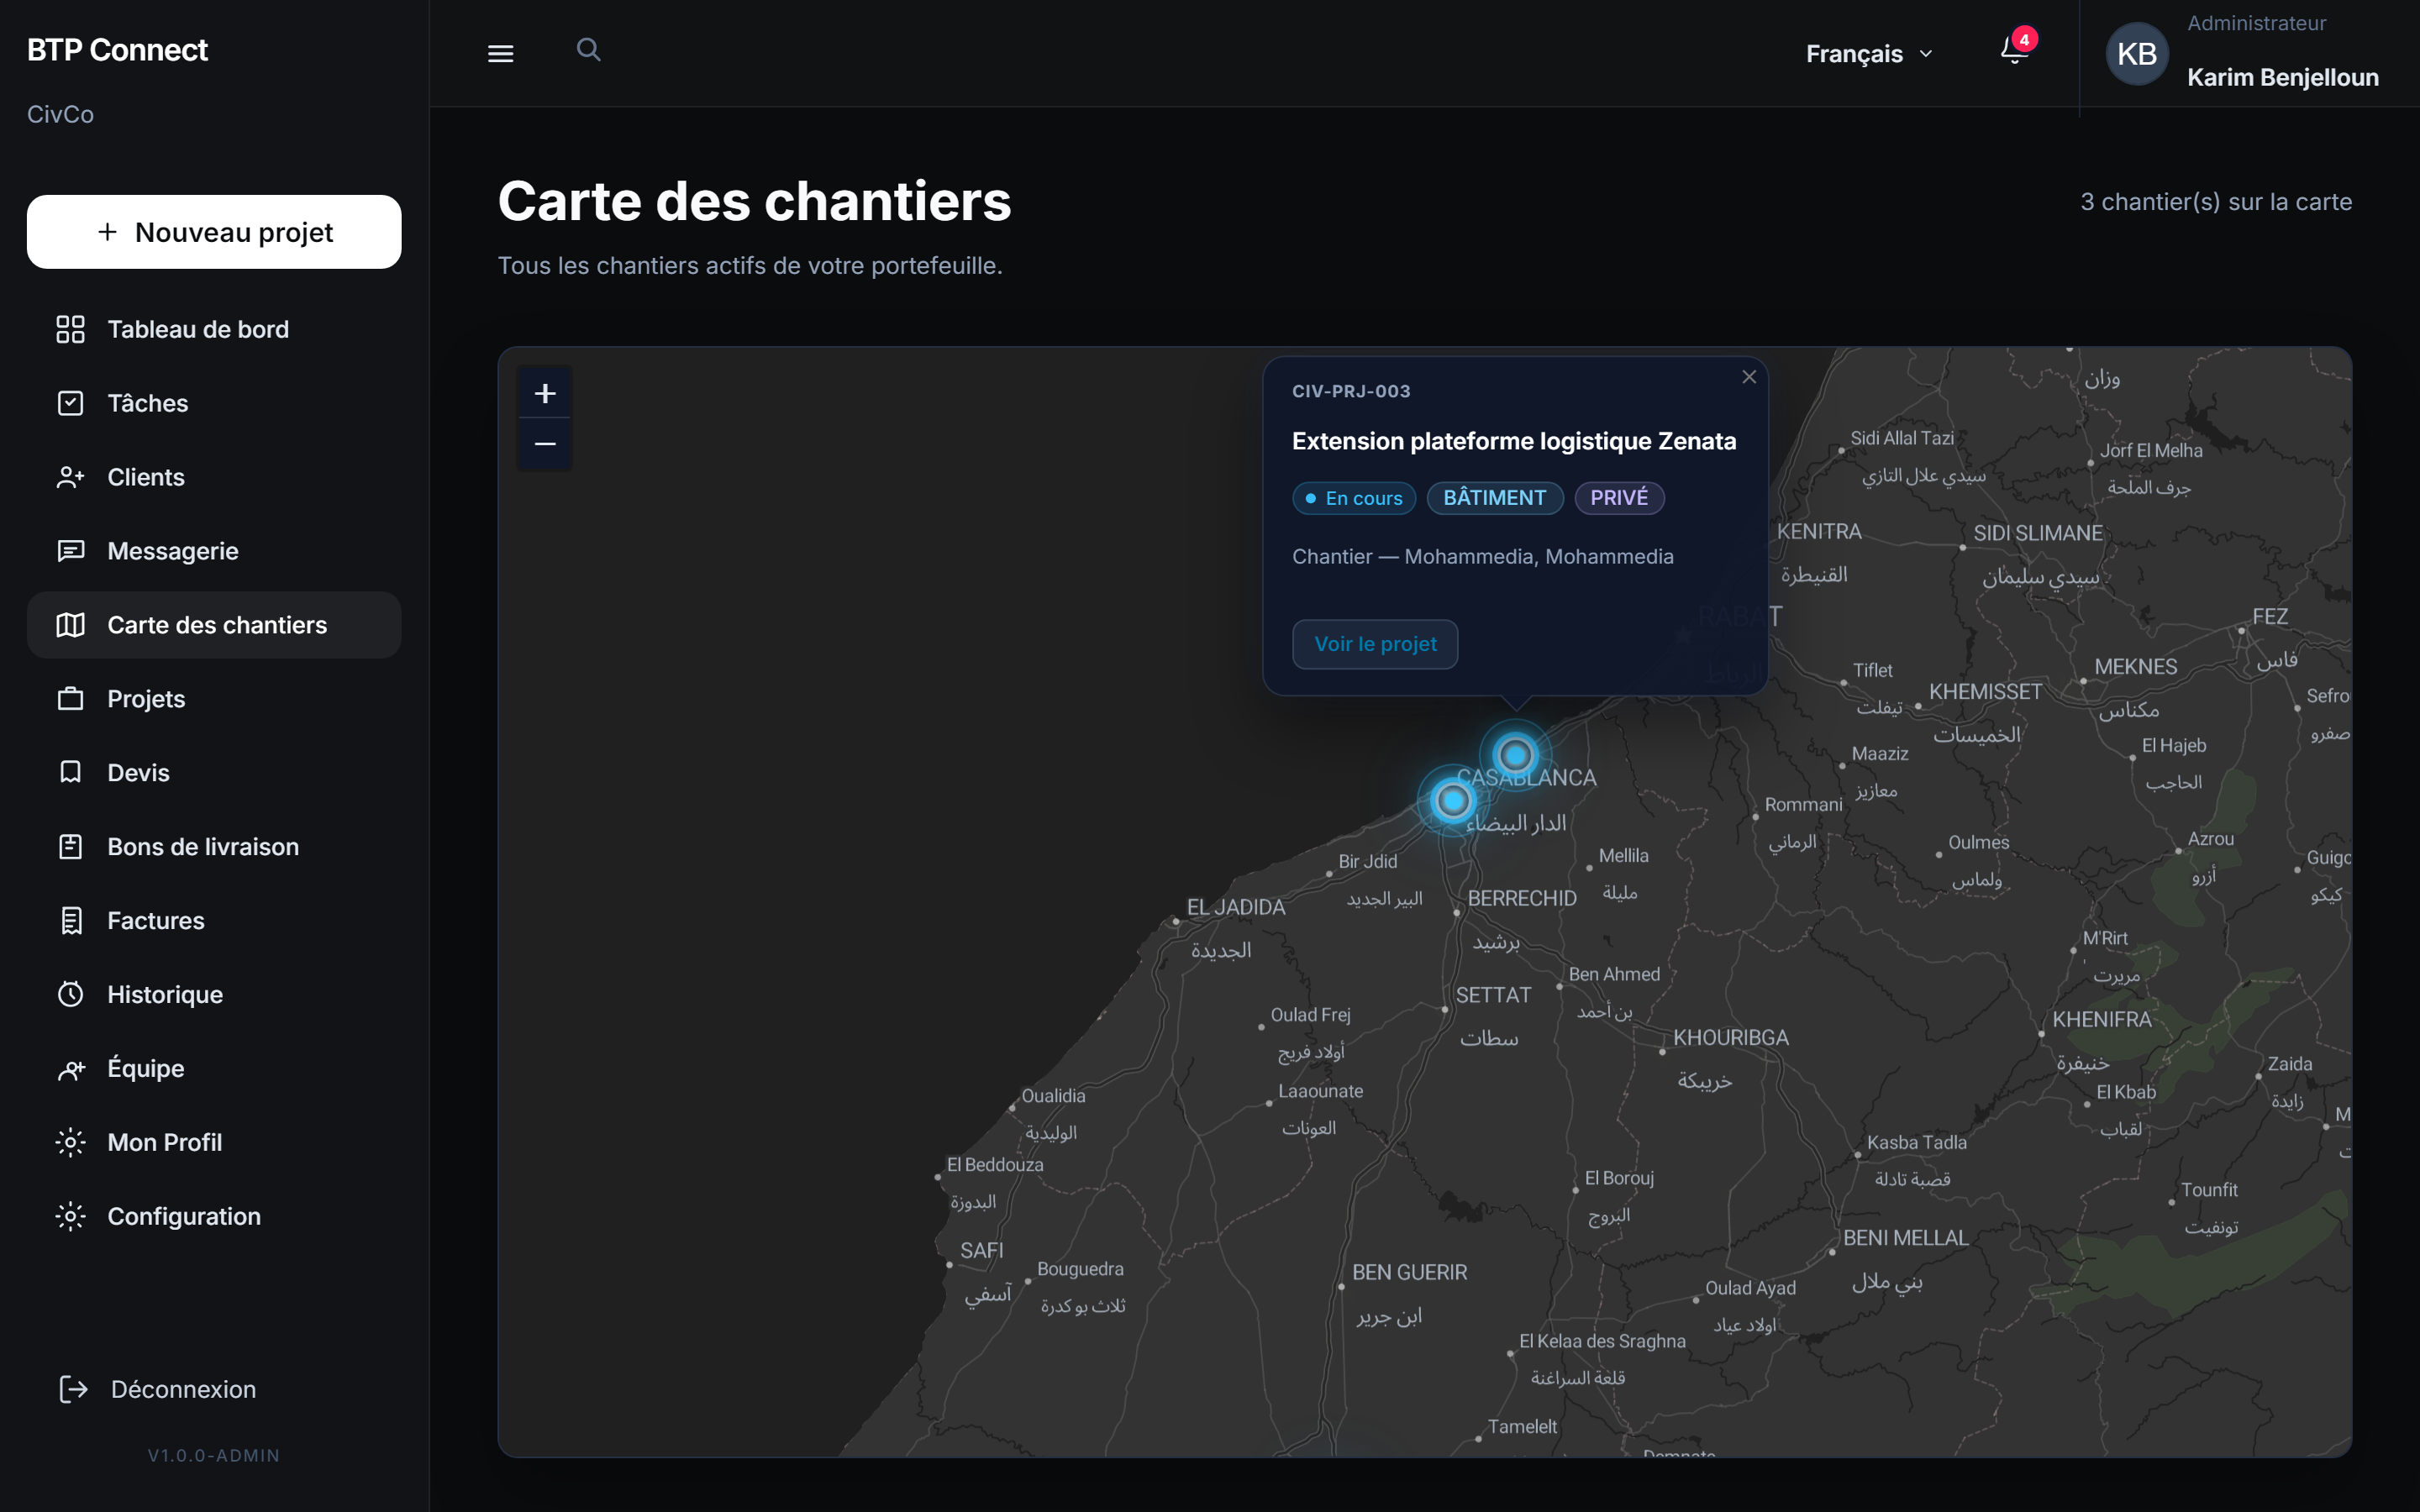
\includegraphics[width=\textwidth]{map.png}
  \caption{Carte des projets : visualisation géographique des chantiers (Leaflet)}
  \label{fig:map}
\end{figure}

La carte (Figure~\ref{fig:map}) affiche les projets géolocalisés sur une carte
interactive Leaflet, utile pour visualiser la répartition géographique des
chantiers de CIVCO BTP.

\medskip

Chaque marqueur sur la carte correspond à un projet géolocalisé. Un clic affiche un
résumé (référence, client, statut, avancement) et un lien vers la fiche détail.
Cette visualisation est particulièrement utile pour la direction et les chefs de
projet qui gèrent plusieurs chantiers répartis sur différentes zones géographiques
du Grand Casablanca et au-delà.

\subsection{Portail client}

\begin{figure}[H]
  \centering
  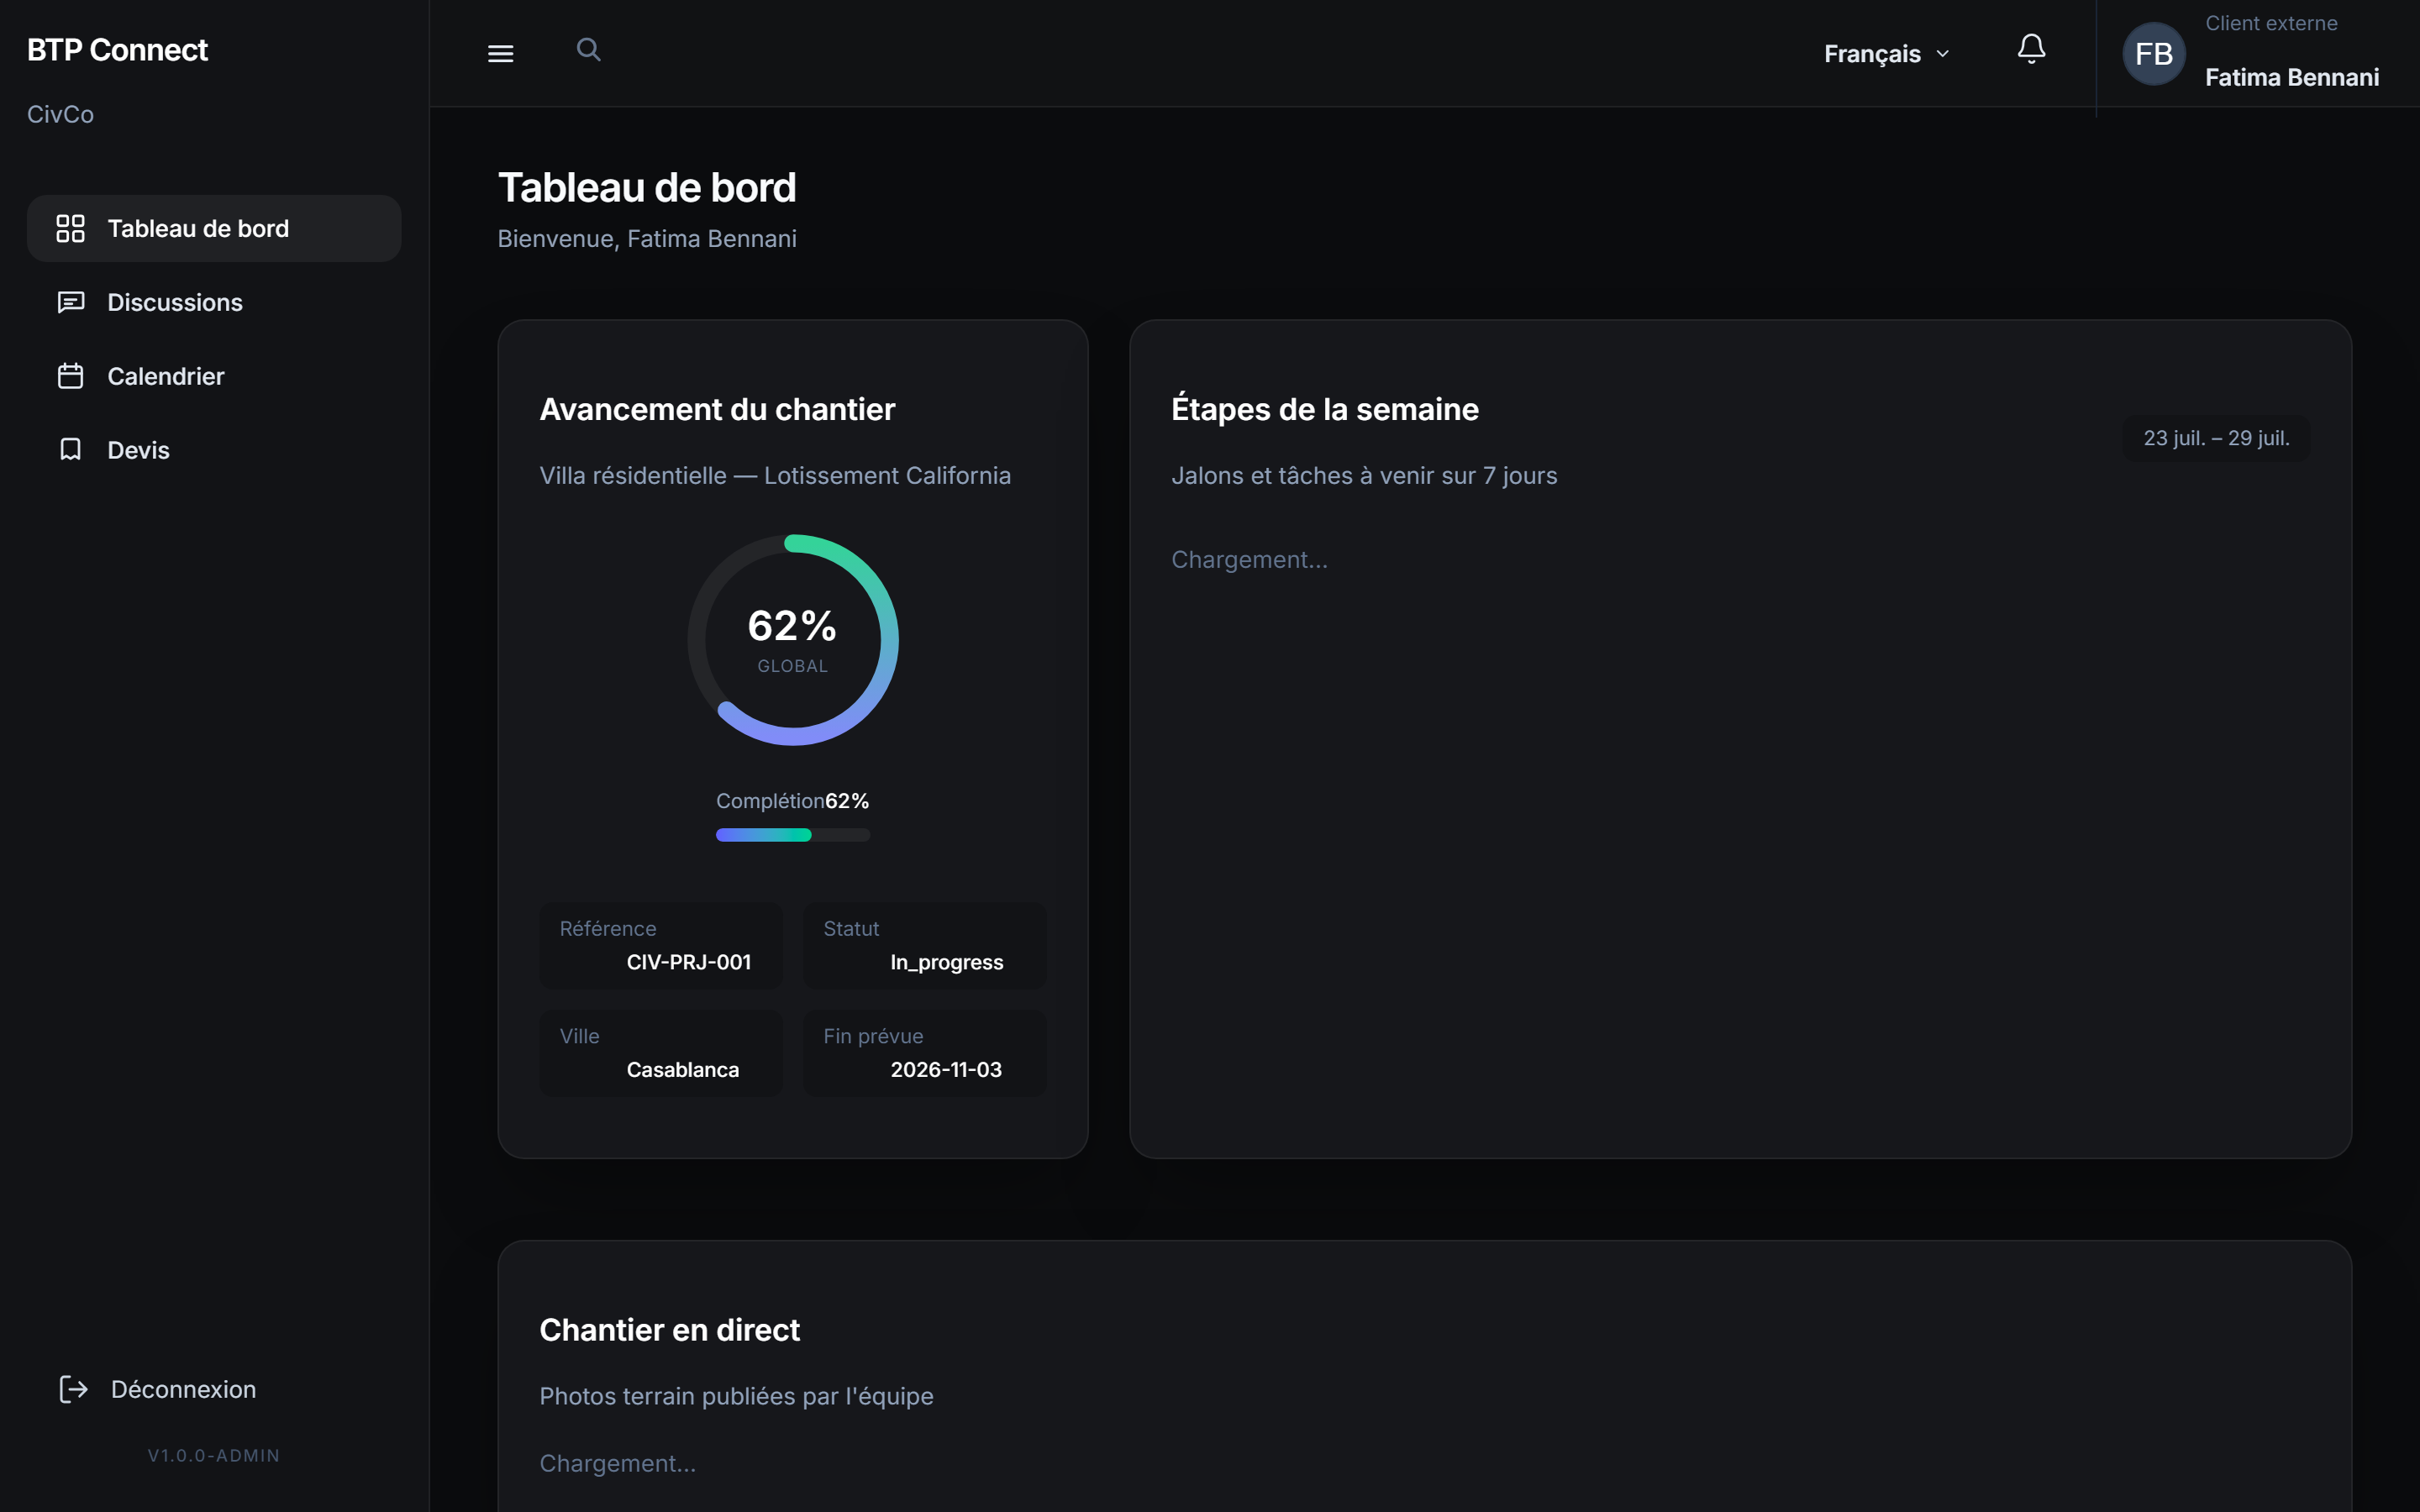
\includegraphics[width=\textwidth]{portal.png}
  \caption{Portail client : consultation des projets, acceptation de devis et signature}
  \label{fig:portal}
\end{figure}

Le portail client (Figure~\ref{fig:portal}) offre une interface simplifiée aux
clients externes : consultation de l'avancement, acceptation de devis, signature
de contrats et messagerie avec l'équipe projet.

\medskip

L'interface portail est volontairement distincte de l'ERP interne : navigation
réduite à quatre entrées (tableau de bord, discussions, calendrier, devis), sans
accès aux modules de gestion internes (projets, facturation, configuration).
Les routes React sont regroupées sous le préfixe \texttt{/portal/*} et protégées
par le middleware d'authentification ; un utilisateur possédant le rôle
\texttt{client\_extern} est automatiquement redirigé vers le portail après
connexion, tandis qu'un collaborateur interne ne peut pas y accéder.

\medskip

\textbf{Tableau de bord client.} L'écran principal (Figure~\ref{fig:portal})
présente trois blocs d'information. Le widget \textit{Avancement du chantier}
affiche un indicateur circulaire (\texttt{ProgressRing}) alimenté par le champ
\texttt{progress\_percent} du projet, accompagné de la référence chantier, du
statut, de la ville et de la date de fin prévue. Le panneau \textit{Étapes de
la semaine} liste les jalons et tâches à échéance sur les sept prochains jours,
filtrés par projet sélectionné. Enfin, le fil \textit{Chantier en direct}
(\texttt{ChantierLiveFeed}) expose les photos terrain publiées par l'équipe
CIVCO BTP, rafraîchies périodiquement pour offrir une visibilité continue
sur l'avancement des travaux.

\medskip

\textbf{Parcours documentaire et contractuel.} Depuis l'onglet \textit{Devis},
le client consulte les propositions commerciales qui le concernent et peut
accepter un devis en un clic ; le statut est immédiatement mis à jour côté
serveur. Pour les contrats, le composant \texttt{ClientContractSignature}
intègre un pad de signature tactile (canvas HTML5) : la signature est capturée,
transmise à l'API et associée au document contractuel, déclenchant la mise à
jour du statut et la notification de l'équipe projet.

\medskip

\textbf{Provisionnement et sécurité.} L'accès portail est créé par
l'administrateur depuis la fiche client (module Clients, Chapitre~4) : un
identifiant de connexion est généré, associé au client concerné via le champ
\texttt{client\_id} de l'utilisateur, et activé ou désactivé à la demande.
Toutes les requêtes API du portail sont filtrées par ce lien client $\rightarrow$
projet : un client externe ne voit que ses propres chantiers, devis et
échanges, conformément au principe de moindre privilège défini au Chapitre~3.

\subsection{Configuration}

\begin{figure}[H]
  \centering
  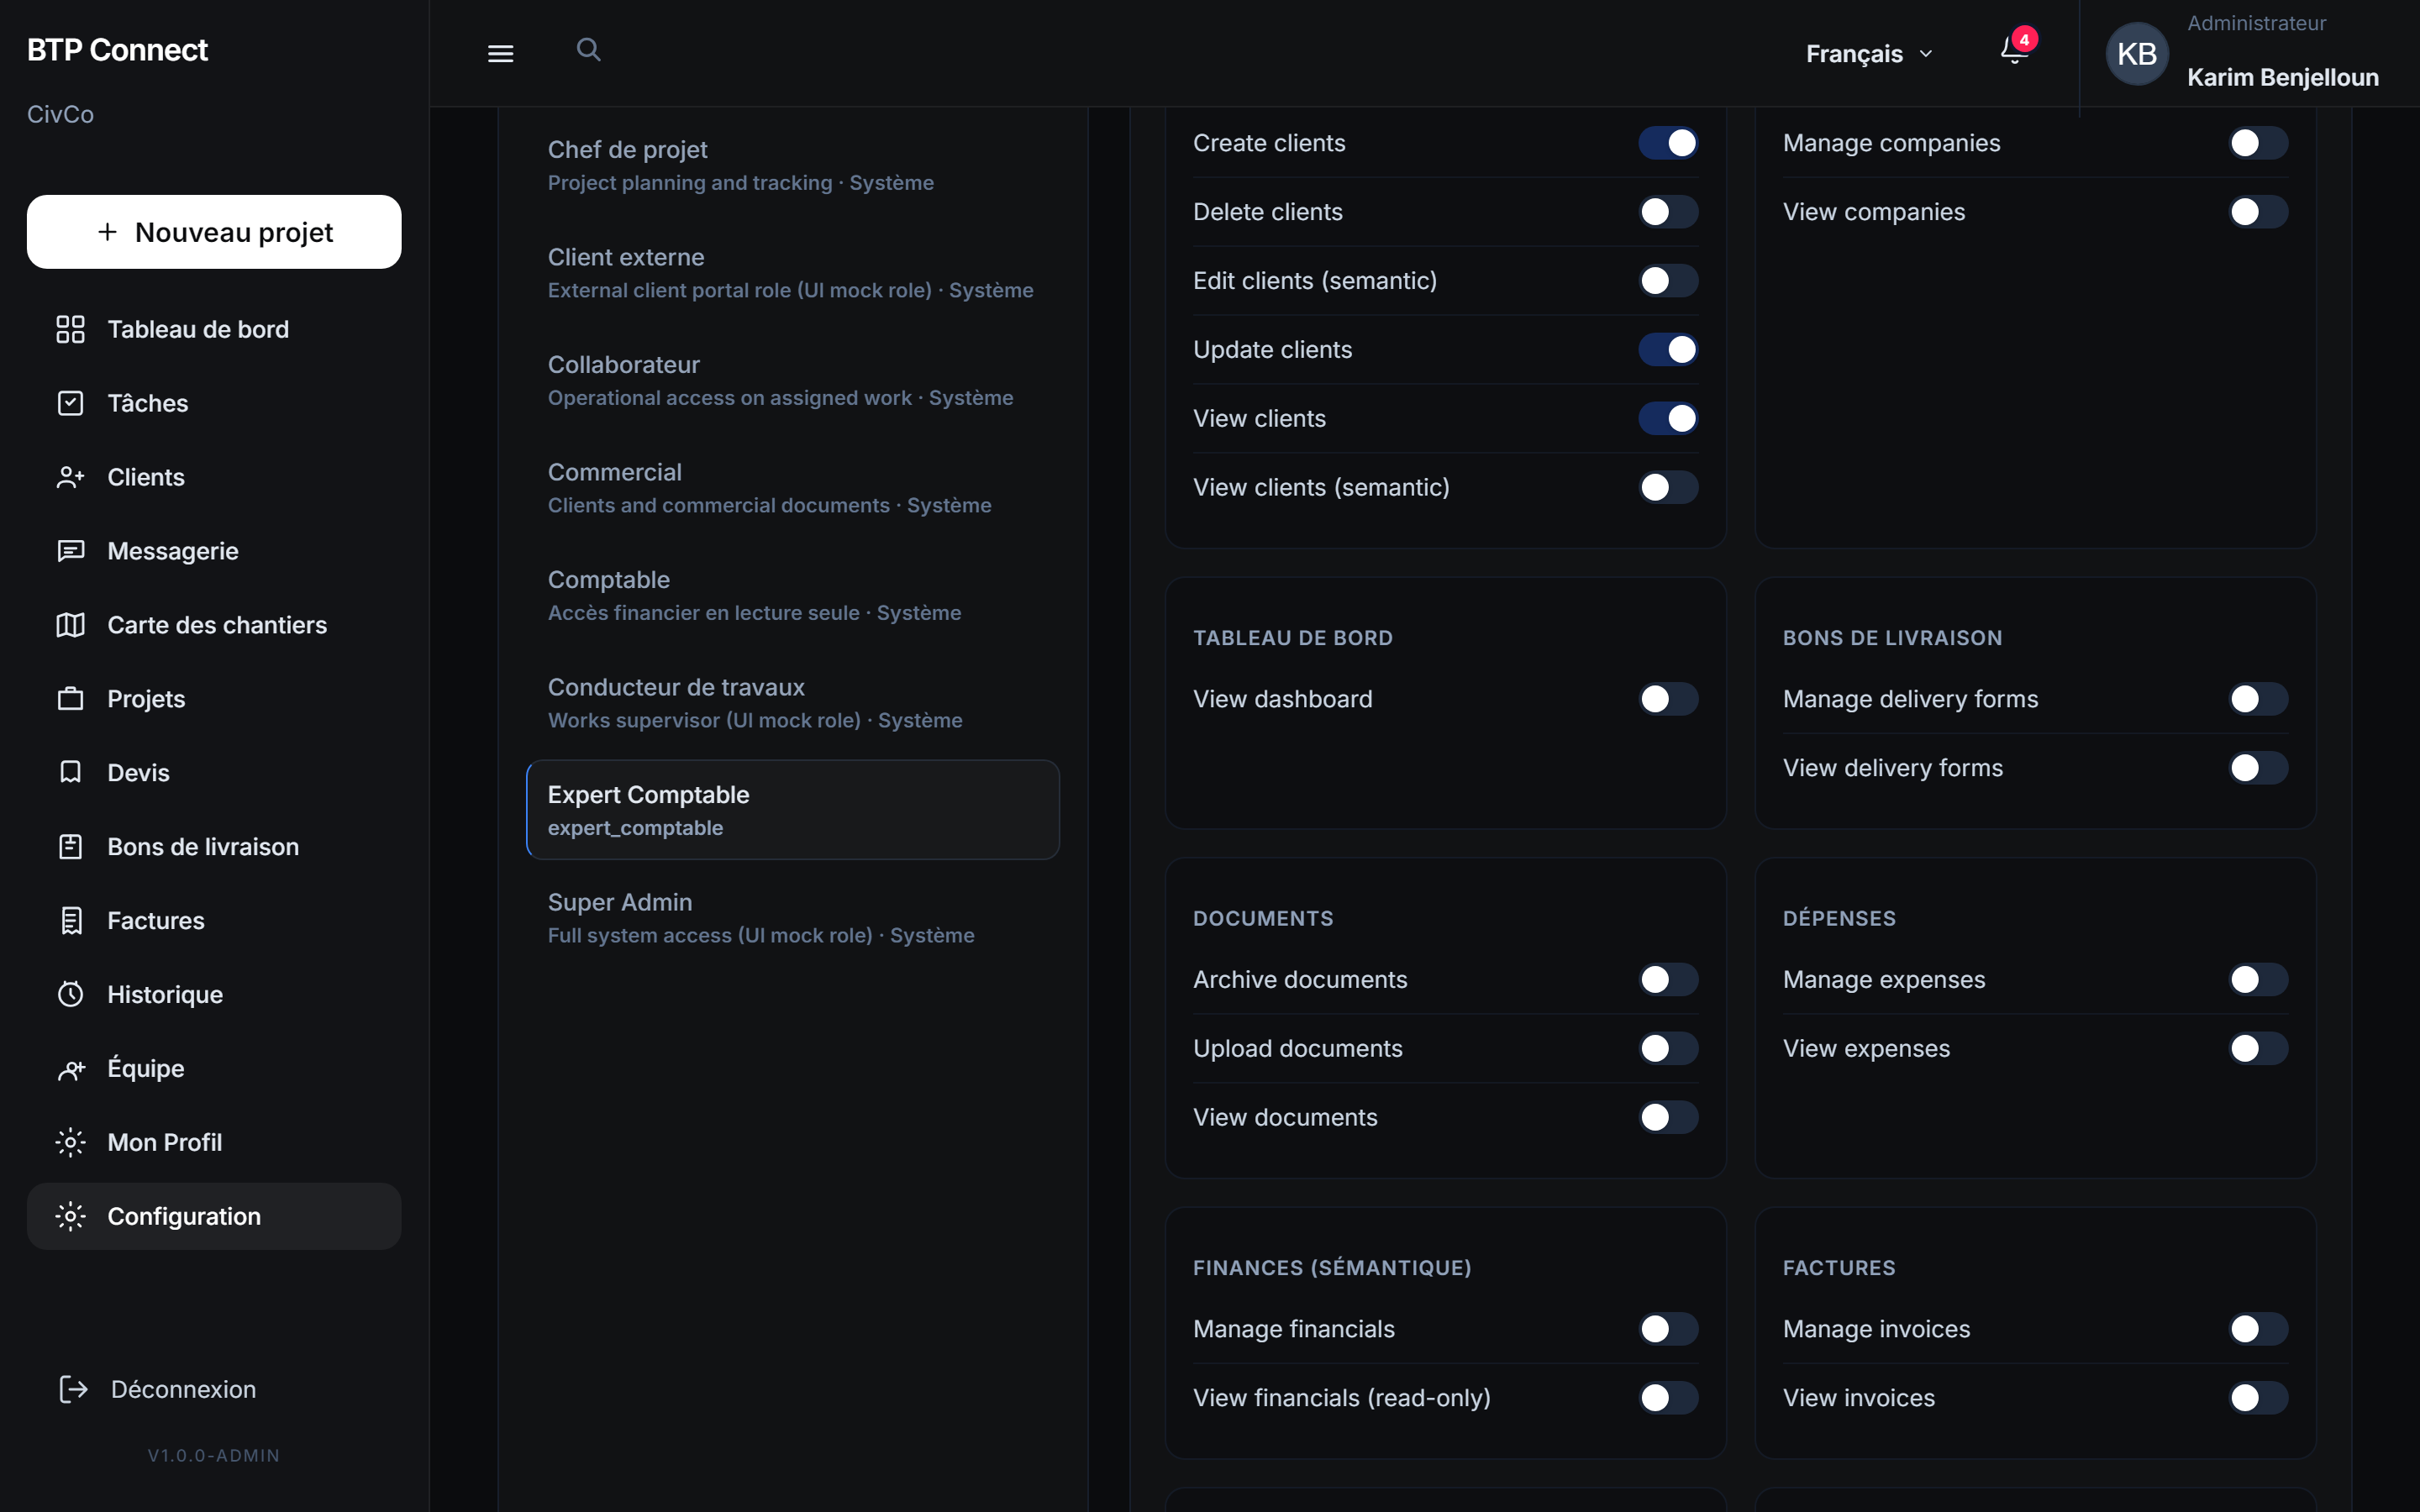
\includegraphics[width=\textwidth]{config.png}
  \caption{Module Configuration : rôles, modèles de documents, contrôles d'impression}
  \label{fig:config}
\end{figure}

Le module Configuration (Figure~\ref{fig:config}) est réservé à l'administrateur :
gestion des rôles et permissions, modèles de contrats et documents, paramètres
d'impression, thème visuel et référentiels (badges, lots, secteurs).

\medskip

Le panneau de configuration est organisé en onglets thématiques : rôles et permissions,
modèles de contrats, contrôles d'impression, modèles de documents et paramètres
généraux. L'administrateur peut créer un nouveau rôle métier, lui attribuer un
sous-ensemble de permissions et l'assigner aux utilisateurs concernés, sans
intervention technique sur le code.

% ─────────────────────────────────────────────────────────────────────
\section{Tests et validation}

La validation de l'application s'appuie sur deux dispositifs complémentaires : une
\textbf{suite de tests automatisés} PHPUnit au niveau du backend, et une
\textbf{campagne de tests manuels} couvrant les parcours utilisateurs de bout en bout.

\subsection{Tests automatisés backend}

Le projet inclut une suite de tests d'intégration PHPUnit dans \texttt{tests/Feature/} :

\begin{description}
  \item[AuthTest] Connexion, déconnexion, accès au profil utilisateur, rejet des
  identifiants invalides.
  \item[ClientProjectTest] CRUD clients et projets, relations, contraintes d'accès.
  \item[QuoteInvoiceTest] Création de devis, lignes de détail, conversion en facture,
  calcul des totaux.
  \item[DocumentTest] Upload et gestion des documents attachés aux projets.
  \item[ExpenseTest] Enregistrement des dépenses de chantier.
  \item[DashboardTest] Agrégation des indicateurs du tableau de bord.
  \item[RoleAccessTest] Vérification des redirections post-login et des permissions
  par profil (comptable, commercial, chef de projet, administrateur).
\end{description}

Les tests utilisent \texttt{RefreshDatabase} et les seeders de démonstration pour
garantir un environnement isolé et reproductible. La commande \texttt{php artisan test}
exécute l'ensemble de la suite.

\subsection{Campagne de tests manuels}

Une checklist de tests manuels a été établie pour valider les parcours que les tests
automatisés ne couvrent pas entièrement :

\begin{itemize}
  \item \textbf{Authentification} : connexion, déconnexion, expiration de session,
  redirection selon le profil.
  \item \textbf{Projets} : création complète (client, phases, équipe, géolocalisation),
  modification, consultation par un utilisateur non-admin.
  \item \textbf{Documents commerciaux} : cycle devis $\rightarrow$ acceptation $\rightarrow$
  facture $\rightarrow$ paiement ; impression avec et sans en-tête.
  \item \textbf{Contrats} : compilation depuis un modèle, signature portail client.
  \item \textbf{Tâches} : création, assignation, changement de statut, visibilité
  selon les permissions.
  \item \textbf{Portail client} : connexion client, consultation projet, acceptation
  devis, messagerie.
  \item \textbf{Configuration} : création de rôle, attribution de permissions,
  modification du thème.
  \item \textbf{Responsive} : consultation sur poste de bureau et tablette.
\end{itemize}

\subsection{Validation qualitative}

L'application a été validée en conditions réelles au sein de CIVCO BTP, avec les
observations suivantes :

\begin{itemize}
  \item \textbf{Adéquation métier} : les modules couvrent les processus quotidiens
  identifiés au Chapitre~1 (suivi de chantier, production documentaire, planification).
  \item \textbf{Ergonomie} : l'interface sombre et la navigation par sidebar ont été
  appréciées par les testeurs internes pour un usage prolongé.
  \item \textbf{Performance} : les listes et fiches détail se chargent en moins de
  500~ms en environnement local ; le tableau de bord agrège les indicateurs sans
  latence perceptible.
  \item \textbf{Sécurité} : les tests de contournement de permissions (accès direct
  à une URL sans droit) sont correctement bloqués côté API avec une réponse
  \texttt{403 Forbidden}.
  \item \textbf{Impression} : le mécanisme de suivi des copies officielles et le
  filigrane « COPIE - NON OFFICIEL » fonctionnent conformément aux exigences métier.
\end{itemize}

\subsection{Synthèse des tests}

Le Tableau~\ref{tab:test_summary} récapitule la couverture de validation par module.

\begin{table}[H]
\caption{Synthèse de la couverture de tests par module}
\label{tab:test_summary}
\centering
\small
\begin{tabular}{|l|c|c|p{5.5cm}|}
\hline
\textbf{Module} & \textbf{Auto.} & \textbf{Manuel} & \textbf{Points vérifiés} \\
\hline
Authentification & $\checkmark$ & $\checkmark$ & Login, logout, session, redirection \\
\hline
Projets & $\checkmark$ & $\checkmark$ & CRUD, phases, équipe, carte \\
\hline
Clients & $\checkmark$ & $\checkmark$ & CRUD, archivage, portail \\
\hline
Devis / Factures & $\checkmark$ & $\checkmark$ & Lignes, conversion, impression \\
\hline
Tâches & --- & $\checkmark$ & Assignation, statuts, permissions \\
\hline
Contrats & --- & $\checkmark$ & Compilation, signature, avenants \\
\hline
Configuration & --- & $\checkmark$ & Rôles, modèles, thème \\
\hline
Portail client & --- & $\checkmark$ & Consultation, acceptation, messagerie \\
\hline
\end{tabular}
\end{table}

% ─────────────────────────────────────────────────────────────────────
\section{Difficultés rencontrées et solutions}

\subsection{Gestion des permissions granulaires}

La mise en place du \textbf{RBAC} avec plus de trente permissions a nécessité une
coordination entre le backend (middleware, seeders) et le frontend (PermissionGate,
routePermissions). La solution retenue centralise la résolution des permissions
dans \texttt{AuthContextService} côté API et \texttt{permissionResolver.js} côté
React, garantissant une source de vérité unique.

\subsection{Impression documentaire}

La génération de PDF côté client (composants React dédiés) et le suivi des quotas
d'impression officielle ont demandé un mécanisme de comptage persistant
(\texttt{PrintTrackingService}) et une interface de choix avant chaque impression
(\texttt{PrintOptionsModal}).

\subsection{Géolocalisation des chantiers}

L'intégration de la carte Leaflet avec géocodage automatique des adresses de chantier
a été réalisée via \texttt{SiteGeocodingService}, qui interroge l'API Nominatim avec
un repli sur un référentiel de coordonnées des villes marocaines
(\texttt{MoroccoCityCoordinates}) en cas d'échec.

\subsection{Synchronisation frontend / backend}

La cohérence entre les permissions affichées dans l'interface et celles vérifiées
côté API a nécessité un travail de synchronisation : chaque route frontend dans
\texttt{routePermissions.js} doit correspondre à un contrôle \texttt{permission:*}
sur l'endpoint associé. Les tests \texttt{RoleAccessTest} et les tests manuels
multi-profils ont permis de détecter et corriger les écarts.

\section*{Conclusion}

Ce chapitre a présenté la réalisation concrète de l'application de gestion de
projets BTP développée pour CIVCO BTP. Au-delà de la conception formalisée au
chapitre précédent, nous avons décrit l'environnement d'exécution, l'organisation
du code, les modules livrés et les dispositifs de validation retenus pour garantir
la fiabilité de la solution en conditions d'usage réelles.

\medskip

\textbf{Environnement et architecture.} L'application repose sur une stack
\textbf{Laravel 13 / React 19 / Vite / MySQL}, orchestrée en développement par
deux processus parallèles (\texttt{php artisan serve} et \texttt{npm run dev}).
Le proxy Vite assure la communication transparente entre la SPA et l'API, tandis
que \textbf{Laravel Sanctum} gère l'authentification par session sécurisée.
Cette séparation frontend / backend a permis de maintenir une frontière nette :
l'interface React ne contient aucune règle métier critique ; la validation, les
calculs financiers et la persistance sont systématiquement assurés côté serveur.

\medskip

\textbf{Implémentation backend.} L'API REST expose plus de quarante contrôleurs
sous le préfixe \texttt{/api/v1/}, structurés par domaine (projets, clients,
devis, factures, tâches, contrats, configuration). Chaque endpoint sensible est
protégé par un middleware de permission (\texttt{permission:*}) et validé par
un Form Request dédié. Les services métier (\texttt{PrintTrackingService},
\texttt{DocumentTemplateCompilationService}, \texttt{TeamMemberService}, etc.)
centralisent les règles de gestion, tandis que les API Resources normalisent
les réponses JSON consommées par le frontend.

\medskip

\textbf{Interface utilisateur.} Le frontend React est organisé en modules par
domaine fonctionnel, avec une sidebar filtrée selon le profil connecté. Les
écrans principaux ont été implémentés et illustrés dans ce chapitre :
authentification (Figure~\ref{fig:login}), tableau de bord
(Figure~\ref{fig:dashboard}), gestion des projets et des clients
(Figures~\ref{fig:projects} et~\ref{fig:clients}), documents commerciaux
(Figures~\ref{fig:quotes} et~\ref{fig:invoices}), planification des tâches
(Figure~\ref{fig:tasks}), carte géographique des chantiers (Figure~\ref{fig:map}),
portail client (Figure~\ref{fig:portal}) et module de configuration
(Figure~\ref{fig:config}). Cette couverture correspond au périmètre fonctionnel
défini au Chapitre~3 et aux processus quotidiens de CIVCO BTP.

\medskip

\textbf{Validation et déploiement.} La qualité de la solution est assurée par
une suite de tests PHPUnit (authentification, CRUD métier, conversion
devis $\rightarrow$ facture, contrôle d'accès par rôle) complétée par une
campagne de tests manuels sur les parcours de bout en bout. L'étude comparative
d'hébergement a orienté le choix vers \textbf{o2switch}, retenu pour sa simplicité
de mise en production, son support francophone et son rapport qualité/prix adapté
à une PME du secteur BTP.

\medskip

\textbf{Bilan.} Les principales difficultés --- permissions granulaires,
impression documentaire, géolocalisation des chantiers et synchronisation
frontend / backend --- ont été résolues par des services dédiés et une
source de vérité unique côté API. L'application est fonctionnelle, testée et
prête pour un déploiement chez CIVCO BTP. Le chapitre suivant conclut ce rapport
en synthétisant les apports du projet et en esquissant les perspectives
d'évolution (notifications temps réel, application mobile, intégration comptable).

\newpage

\chapter*{Conclusion Générale et Perspectives}
\addcontentsline{toc}{chapter}{Conclusion Générale et Perspectives}
\markboth{Conclusion Générale et Perspectives}{Conclusion Générale et Perspectives}

Ce projet de fin d'études avait pour objectif de concevoir et développer une
application web de gestion et de planification des projets de construction pour
\textbf{CIVCO BTP}, afin de centraliser les processus métier dispersés entre
tableurs, documents papier et échanges informels.

\medskip

L'application développée au cours de ce stage constitue une réponse concrète et
fonctionnelle à cette problématique. Les réalisations techniques couvrent
l'intégralité du cycle de vie d'un projet de construction :

\begin{itemize}
  \item \textbf{Gestion de projets} : création et suivi des chantiers par phases,
  affectation des équipes, géolocalisation sur carte interactive, suivi de
  l'avancement et des dépenses.
  \item \textbf{Relation client} : fiches clients centralisées, archivage, portail
  dédié pour consultation et validation des documents.
  \item \textbf{Documents commerciaux} : production de devis, factures et bons de
  livraison avec lignes de détail, conversion automatisée et suivi des impressions
  officielles.
  \item \textbf{Suivi contractuel} : gestion des contrats et avenants, compilation
  depuis des modèles, signature électronique côté client.
  \item \textbf{Planification opérationnelle} : tâches assignées par projet et par
  collaborateur, tableau de bord avec indicateurs et graphiques.
  \item \textbf{Sécurité et gouvernance} : authentification Sanctum, contrôle
  d'accès par rôles et permissions (RBAC), journal d'activité pour la traçabilité.
  \item \textbf{Architecture technique} : backend Laravel 13 exposant une API REST,
  frontend React 19 en SPA, base de données relationnelle, plus de soixante-dix
  migrations et une suite de tests PHPUnit.
\end{itemize}

\section*{Bilan du projet}

Sur le plan fonctionnel, l'application répond aux besoins identifiés lors de la
phase d'analyse : chaque service de CIVCO BTP dispose désormais d'un point d'accès
unique pour consulter et mettre à jour les informations liées aux chantiers. La
centralisation des données élimine les ressaisies manuelles entre tableurs et
documents isolés, et le tableau de bord offre une visibilité en temps réel sur
l'activité de l'entreprise.

\medskip

Sur le plan technique, les choix Laravel + React se sont révélés pertinents pour
ce type d'application métier : Laravel fournit une base solide pour l'API, la
sécurité et la persistance, tandis que React permet de construire une interface
réactive et modulaire. L'architecture en trois couches facilite la maintenance
et l'ajout de nouveaux modules sans remettre en cause l'existant.

\medskip

Sur le plan méthodologique, l'approche itérative adoptée pendant le stage ---
analyse des besoins, conception, développement par modules, tests et validation
--- a permis de livrer des incréments fonctionnels démontrables à chaque réunion
de suivi avec l'encadrant professionnel, M. Mohamed BENABDELLAH-CHAOUNI, et
l'encadrant pédagogique, le Pr. Mohammed El Assad.

\section*{Apports personnels et compétences acquises}

Ce stage au sein de CIVCO BTP m'a permis de consolider et d'approfondir
plusieurs compétences techniques et transversales :

\begin{itemize}
  \item \textbf{Développement full-stack} : conception et implémentation d'une
  application complète, de la base de données à l'interface utilisateur.
  \item \textbf{Architecture logicielle} : application des patrons MVC, services
  métier, API REST et SPA dans un contexte professionnel réel.
  \item \textbf{Sécurité applicative} : mise en œuvre concrète de l'authentification,
  du RBAC, de la protection CSRF et de la journalisation.
  \item \textbf{Modélisation} : rédaction de spécifications fonctionnelles,
  diagrammes UML et modèle de données relationnel.
  \item \textbf{Gestion de projet} : planification, priorisation des fonctionnalités,
  suivi Kanban via Trello, communication régulière avec les parties prenantes.
  \item \textbf{Rigueur documentaire} : rédaction du présent rapport et documentation
  technique du code produit.
\end{itemize}

\medskip

Au-delà des compétences techniques, ce projet m'a sensibilisé aux réalités du
secteur BTP au Maroc : la diversité des intervenants sur un chantier, l'importance
de la traçabilité documentaire et les contraintes de terrain qui influencent les
choix ergonomiques de l'application.

\section*{Limites et axes d'amélioration}

Malgré les résultats obtenus, certaines limites subsistent et ouvrent des pistes
d'amélioration :

\begin{itemize}
  \item \textbf{Couverture de tests} : la suite PHPUnit couvre les flux critiques
  mais ne teste pas encore l'ensemble des modules (contrats, portail client).
  L'ajout de tests end-to-end (Cypress, Playwright) renforcerait la confiance
  avant un déploiement en production.
  \item \textbf{Performance à l'échelle} : les tests ont été réalisés en
  environnement local avec un volume de données modéré. Un benchmark sur des
  milliers de projets et documents serait nécessaire avant un usage intensif.
  \item \textbf{Formation utilisateurs} : l'adoption de l'outil par l'ensemble des
  services nécessitera un accompagnement au changement et une documentation
  utilisateur dédiée.
  \item \textbf{Déploiement production} : une étude comparative OVHcloud / o2switch a
  conduit au choix d'\textbf{o2switch} ; la mise en ligne effective reste à finaliser
  (configuration du domaine, déploiement du build React et exécution des migrations).
\end{itemize}

\section*{Perspectives}

L'application offre plusieurs pistes d'évolution à court et moyen terme pour CIVCO BTP.

\medskip

\textbf{Évolutions fonctionnelles :}
\begin{itemize}
  \item \textbf{Application mobile} : version allégée pour les conducteurs de travaux
  sur chantier (consultation des tâches, mise à jour d'avancement, photos).
  \item \textbf{Business Intelligence} : tableaux de bord avancés, export Excel/PDF
  des indicateurs, analyse de la rentabilité par projet.
  \item \textbf{Gestion des stocks} : suivi des matériaux et approvisionnements liés
  aux chantiers.
  \item \textbf{Notifications} : alertes email ou push pour les échéances de tâches,
  validations en attente et paiements.
  \item \textbf{Signature avancée} : intégration d'un prestataire de signature
  électronique qualifiée pour les contrats à forte valeur juridique.
\end{itemize}

\textbf{Évolutions techniques :}
\begin{itemize}
  \item \textbf{Déploiement production (o2switch)} : publication de l'application sur
  l'hébergement retenu (build React, configuration Laravel, certificat SSL, sauvegardes
  automatiques de la base MySQL).
  \item \textbf{Montée en charge} : si le volume d'utilisateurs augmente significativement,
  migration vers une offre VPS OVHcloud ou cloud managé pour plus de flexibilité.
  \item \textbf{Tests} : extension de la couverture PHPUnit, ajout de tests
  end-to-end (Cypress ou Playwright) sur les parcours critiques.
  \item \textbf{Performance} : mise en cache des requêtes fréquentes (Redis),
  pagination optimisée sur les grandes listes.
  \item \textbf{CI/CD} : pipeline d'intégration continue (GitHub Actions) pour
  exécuter les tests automatiquement à chaque commit.
\end{itemize}

\medskip

Ce projet illustre comment une architecture web moderne (Laravel + React) peut
transformer la gestion quotidienne d'une entreprise du BTP, en remplaçant des outils
dispersés par une plateforme intégrée, sécurisée et adaptée aux profils métier de
l'organisation. L'application constitue une base solide sur laquelle CIVCO BTP peut
continuer à digitaliser et optimiser ses processus internes, au service de la qualité
de ses études et du suivi de ses chantiers.

\newpage


% ── Bibliography ─────────────────────────────────────────────
\nocite{*}
\printbibliography[heading=bibintoc, title={Bibliographie et Webographie}]
\newpage

% ── Appendix ─────────────────────────────────────────────────
\appendix
\makeatletter
\renewcommand{\@makechapterhead}[1]{%
  \vspace*{50\p@}%
  {\parindent \z@ \raggedright \normalfont
    \Huge\bfseries Annexe~: #1\par\nobreak
    \vskip 40\p@
  }}
\makeatother
\renewcommand{\cftchappresnum}{Annexe~}
\renewcommand{\cftchapaftersnum}{}
% ─────────────────────────────────────────────────────────────────────
%   ANNEXES
% ─────────────────────────────────────────────────────────────────────

% Configuration globale des listings de code
\lstset{
  basicstyle=\ttfamily\footnotesize,
  breaklines=true,
  breakatwhitespace=false,
  columns=fullflexible,
  keepspaces=true,
  showstringspaces=false,
  tabsize=2,
  frame=single,
  rulecolor=\color{ensamBlue!40},
  backgroundcolor=\color{ensamBlue!3},
  xleftmargin=0.5cm,
  xrightmargin=0.5cm,
  keywordstyle=\color{ensamBlue}\bfseries,
  stringstyle=\color{orange!70!black},
  commentstyle=\color{gray}\itshape,
  numberstyle=\tiny\color{gray},
  numbers=left,
  numbersep=6pt,
  captionpos=b,
}

\chapter{Annexes}

% =====================================================================
\section{Extraits de code source}

Cette annexe présente les extraits de code source les plus représentatifs de
l'application développée pour CIVCO BTP, sélectionnés pour illustrer les
contributions techniques décrites dans ce rapport.

% ─────────────────────────────────────────────────────────────────────
\subsection{Authentification API (\texttt{AuthController.php})}

Le contrôleur d'authentification gère la connexion des utilisateurs internes
via Laravel Sanctum. La méthode \texttt{login} valide les identifiants, régénère
la session et retourne le contexte utilisateur (profil, rôles, permissions).

\begin{lstlisting}[language=PHP,
  caption={AuthController.php : connexion utilisateur (extrait)}]
public function login(LoginRequest $request,
    AuthContextService $authContext): JsonResponse
{
    $credentials = $request->only('email', 'password');

    if (! Auth::attempt($credentials, $request->boolean('remember'))) {
        throw ValidationException::withMessages([
            'email' => [__('auth.failed')],
        ]);
    }

    $user = Auth::user();

    if (! $user->canAccessApplication()) {
        Auth::logout();
        throw ValidationException::withMessages([
            'email' => [CheckUserStatus::DEACTIVATED_MESSAGE],
        ]);
    }

    if ($request->hasSession()) {
        $request->session()->regenerate();
    }

    return response()->json($authContext->forUser($user));
}
\end{lstlisting}

% ─────────────────────────────────────────────────────────────────────
\subsection{Conversion devis vers facture (\texttt{QuoteService.php})}

Le service métier \texttt{QuoteService} encapsule la logique de conversion d'un
devis accepté en facture. L'opération s'exécute dans une transaction base de
données pour garantir la cohérence des enregistrements.

\begin{lstlisting}[language=PHP,
  caption={QuoteService.php : conversion devis $\rightarrow$ facture (extrait)}]
public function convertToInvoice(Quote $quote,
    ?int $dispatchNoteId = null): Invoice
{
    if ($quote->status !== QuoteStatus::Accepted) {
        throw new InvalidArgumentException(
            'Only accepted quotes can be converted.');
    }

    if ($quote->invoice()->exists()) {
        throw new InvalidArgumentException(
            'This quote has already been converted.');
    }

    return DB::transaction(function () use ($quote, $dispatchNoteId) {
        $quote->load('lines');

        $invoice = Invoice::query()->create([
            'company_id' => $quote->company_id,
            'client_id'  => $quote->client_id,
            'project_id' => $quote->project_id,
            'quote_id'   => $quote->id,
            'reference'  => $this->invoiceReferenceService
                                ->nextForCompany($quote->company_id),
            'status'     => InvoiceStatus::Draft,
            'total_ht'   => $quote->total_ht,
            'total_tax'  => $quote->total_tax,
            'total_ttc'  => $quote->total_ttc,
        ]);

        foreach ($quote->lines as $index => $line) {
            $invoice->lines()->create([
                'sort_order'      => $index + 1,
                'description'     => $line->description,
                'quantity'        => $line->quantity,
                'unit_price_ht'   => $line->unit_price_ht,
                'line_total_ht'   => $line->line_total_ht,
                'line_total_ttc'  => $line->line_total_ttc,
            ]);
        }

        return $invoice->load(['client', 'project', 'lines']);
    });
}
\end{lstlisting}

% ─────────────────────────────────────────────────────────────────────
\subsection{Modèle Projet (\texttt{Project.php})}

Le modèle Eloquent \texttt{Project} centralise les relations métier d'un chantier :
client, phases, équipe, devis et factures.

\begin{lstlisting}[language=PHP,
  caption={Project.php : relations Eloquent (extrait)}]
class Project extends Model
{
    protected $fillable = [
        'company_id', 'client_id', 'reference', 'title',
        'status', 'budget', 'progress_percent',
        'start_date', 'end_date', 'latitude', 'longitude',
    ];

    protected function casts(): array
    {
        return [
            'status' => ProjectStatus::class,
            'start_date' => 'date',
            'end_date' => 'date',
            'budget' => 'decimal:2',
            'progress_percent' => 'decimal:2',
        ];
    }

    public function client(): BelongsTo
    {
        return $this->belongsTo(Client::class);
    }

    public function phases(): HasMany
    {
        return $this->hasMany(ProjectPhase::class);
    }

    public function teamMembers(): BelongsToMany
    {
        return $this->belongsToMany(User::class, 'project_user');
    }

    public function quotes(): HasMany
    {
        return $this->hasMany(Quote::class);
    }
}
\end{lstlisting}

% ─────────────────────────────────────────────────────────────────────
\subsection{Client HTTP frontend (\texttt{client.js})}

Le module \texttt{api/client.js} configure l'instance Axios partagée par tous
les modules frontend. Il transmet les cookies Sanctum, le jeton CSRF et le
contexte société (\texttt{X-Company-Id}).

\begin{lstlisting}[language=Java,
  caption={client.js : configuration Axios et intercepteurs (extrait)}]
const api = axios.create({
  baseURL: import.meta.env.VITE_API_URL ?? '',
  withCredentials: true,
  headers: {
    Accept: 'application/json',
    'Content-Type': 'application/json',
    'X-Requested-With': 'XMLHttpRequest',
  },
})

api.interceptors.request.use(async (config) => {
  if (activeCompanyId) {
    config.headers['X-Company-Id'] = activeCompanyId
  }

  const method = config.method?.toLowerCase()
  if (['post', 'put', 'patch', 'delete'].includes(method)) {
    let token = getCookie('XSRF-TOKEN')
    if (!token) {
      await api.get('/sanctum/csrf-cookie')
      token = getCookie('XSRF-TOKEN')
    }
    if (token) {
      config.headers['X-XSRF-TOKEN'] = token
    }
  }

  return config
})

api.interceptors.response.use(
  (response) => response,
  (error) => {
    if (error.response?.status === 401) {
      window.dispatchEvent(new CustomEvent('auth:unauthorized'))
    }
    return Promise.reject(error)
  }
)
\end{lstlisting}

% =====================================================================
\section{Configuration : variables d'environnement}

Le fichier \texttt{.env} du backend centralise la configuration de l'application.
Le Tableau~\ref{tab:annexe_env} décrit les variables principales utilisées en
développement et en production.

\begin{table}[H]
\caption{Variables d'environnement principales}
\label{tab:annexe_env}
\centering
\small
\begin{tabular}{|l|p{8.5cm}|}
\hline
\textbf{Variable} & \textbf{Rôle} \\
\hline
\texttt{APP\_URL} & URL publique du backend Laravel \\
\hline
\texttt{DB\_CONNECTION} & Pilote SGBD (\texttt{mysql} ou \texttt{pgsql}) \\
\hline
\texttt{DB\_DATABASE} & Nom de la base de données \\
\hline
\texttt{SESSION\_DRIVER} & Stockage des sessions (\texttt{database} recommandé) \\
\hline
\texttt{SANCTUM\_STATEFUL\_DOMAINS} & Domaines autorisés pour les cookies SPA \\
\hline
\texttt{FRONTEND\_URL} & URL du frontend React (CORS et redirections) \\
\hline
\texttt{MAIL\_*} & Configuration SMTP pour les notifications \\
\hline
\end{tabular}
\end{table}

\medskip

Exemple de configuration minimale pour un environnement de développement local :

\lstset{
  language={},
  keywordstyle=\color{black},
  stringstyle=\color{black},
  commentstyle=\color{gray}\itshape,
}

\begin{lstlisting}[caption={.env : configuration de développement (extrait)}]
APP_NAME="CIVCO BTP"
APP_ENV=local
APP_DEBUG=true
APP_URL=http://127.0.0.1:8000

DB_CONNECTION=mysql
DB_HOST=127.0.0.1
DB_PORT=3306
DB_DATABASE=civco_btp
DB_USERNAME=root
DB_PASSWORD=

SESSION_DRIVER=database
SESSION_LIFETIME=120

SANCTUM_STATEFUL_DOMAINS=localhost,127.0.0.1:5173

FRONTEND_URL=http://127.0.0.1:5173

MAIL_MAILER=smtp
MAIL_HOST=smtp.example.com
MAIL_PORT=587
MAIL_USERNAME=null
MAIL_PASSWORD=null
\end{lstlisting}

% =====================================================================
\section{Comptes de démonstration}

Le seeder de démonstration fournit des comptes utilisateurs permettant de
tester les différents profils métier de CIVCO BTP. Le Tableau~\ref{tab:demo_users}
liste les identifiants utilisés en environnement de développement.

\begin{table}[H]
\caption{Comptes de démonstration (mot de passe : \texttt{password})}
\label{tab:demo_users}
\centering
\small
\begin{tabular}{|l|l|p{5.5cm}|}
\hline
\textbf{Email} & \textbf{Profil} & \textbf{Accès principal} \\
\hline
\texttt{admin@civco.ma} & Administrateur & Configuration, tous modules \\
\hline
\texttt{ingenieur@civco.ma} & Chef de projet & Projets, tâches, équipe \\
\hline
\texttt{compta@civco.ma} & Comptable & Factures, paiements \\
\hline
\texttt{chantier@civco.ma} & Chef de chantier & Projets, tâches terrain \\
\hline
\texttt{tech@civco.ma} & Technicien & Tâches assignées, consultation \\
\hline
\end{tabular}
\end{table}

\medskip

Ces comptes sont créés par la commande \texttt{php artisan migrate --seed} et
permettent de valider le contrôle d'accès par rôles décrit au Chapitre~3.

% =====================================================================
\section{Référentiel des endpoints API}

Le Tableau~\ref{tab:api_endpoints} présente les principaux endpoints exposés
sous le préfixe \texttt{/api/v1/}. Toutes les routes (sauf \texttt{login}) sont
protégées par le middleware \texttt{auth:sanctum} et soumises à un contrôle de
permissions.

\begin{table}[H]
\caption{Principaux endpoints de l'API REST}
\label{tab:api_endpoints}
\centering
\footnotesize
\begin{tabular}{|l|l|p{5.5cm}|}
\hline
\textbf{Méthode} & \textbf{Endpoint} & \textbf{Description} \\
\hline
POST & \texttt{/login} & Authentification utilisateur \\
\hline
GET & \texttt{/me} & Profil et permissions de l'utilisateur courant \\
\hline
GET/POST & \texttt{/projects} & Liste et création de projets \\
\hline
GET/PUT & \texttt{/projects/\{id\}} & Consultation et modification d'un projet \\
\hline
GET/POST & \texttt{/clients} & Liste et création de clients \\
\hline
GET/POST & \texttt{/quotes} & Liste et création de devis \\
\hline
POST & \texttt{/quotes/\{id\}/convert} & Conversion devis $\rightarrow$ facture \\
\hline
GET/POST & \texttt{/invoices} & Liste et création de factures \\
\hline
GET/POST & \texttt{/tasks} & Liste et création de tâches \\
\hline
GET/POST & \texttt{/contracts} & Liste et création de contrats \\
\hline
GET & \texttt{/dashboard} & Indicateurs du tableau de bord \\
\hline
GET & \texttt{/search} & Recherche globale (clients, projets, documents) \\
\hline
GET & \texttt{/activity-logs} & Journal des actions (administrateur) \\
\hline
\end{tabular}
\end{table}

% =====================================================================
\section{Schéma des entités principales}

Le Tableau~\ref{tab:entity_schema} décrit les attributs essentiels des entités
métier les plus consultées dans l'application.

\begin{table}[H]
\caption{Attributs principaux des entités métier}
\label{tab:entity_schema}
\centering
\small
\begin{tabular}{|l|p{10.5cm}|}
\hline
\textbf{Entité} & \textbf{Attributs clés} \\
\hline
\texttt{Project} & \texttt{reference}, \texttt{title}, \texttt{status}, \texttt{budget},
\texttt{progress\_percent}, \texttt{start\_date}, \texttt{end\_date},
\texttt{latitude}, \texttt{longitude}, \texttt{client\_id} \\
\hline
\texttt{Client} & \texttt{name}, \texttt{email}, \texttt{phone}, \texttt{status},
\texttt{is\_official}, \texttt{archived\_at} \\
\hline
\texttt{Quote} & \texttt{reference}, \texttt{status}, \texttt{total\_ht},
\texttt{total\_tax}, \texttt{total\_ttc}, \texttt{project\_id}, \texttt{client\_id} \\
\hline
\texttt{Invoice} & \texttt{reference}, \texttt{status}, \texttt{issued\_at},
\texttt{due\_date}, \texttt{amount\_paid}, \texttt{balance\_due}, \texttt{quote\_id} \\
\hline
\texttt{Task} & \texttt{title}, \texttt{status}, \texttt{priority},
\texttt{due\_date}, \texttt{project\_phase\_id}, \texttt{assigned\_to} \\
\hline
\texttt{Contract} & \texttt{reference}, \texttt{status}, \texttt{signed\_at},
\texttt{project\_id}, \texttt{template\_id} \\
\hline
\end{tabular}
\end{table}

\medskip

Les statuts des entités sont implémentés sous forme d'énumérations PHP
(\texttt{ProjectStatus}, \texttt{QuoteStatus}, \texttt{InvoiceStatus},
\texttt{TaskStatus}) garantissant la validité des transitions d'état côté
serveur.

% =====================================================================
\section{Guide de démarrage rapide}

Pour reproduire l'environnement de développement décrit au Chapitre~4, les commandes
suivantes permettent d'initialiser l'application à partir du dépôt source :

\begin{lstlisting}[language={}, caption={Commandes d'initialisation de l'application}]
# Backend
cd backend
composer install
cp .env.example .env
php artisan key:generate
php artisan migrate --seed
php artisan serve

# Frontend (dans un second terminal)
cd frontend
npm install
npm run dev
\end{lstlisting}

\medskip

L'application est alors accessible à l'adresse \texttt{http://127.0.0.1:5173} (frontend)
avec le proxy Vite redirigeant les appels API vers \texttt{http://127.0.0.1:8000}.
Les comptes de démonstration listés en section~3 permettent de tester les différents
profils métier.

\newpage


\end{document}